% Options for packages loaded elsewhere
\PassOptionsToPackage{unicode}{hyperref}
\PassOptionsToPackage{hyphens}{url}
%
\documentclass[
]{book}
\usepackage{amsmath,amssymb}
\usepackage{iftex}
\ifPDFTeX
  \usepackage[T1]{fontenc}
  \usepackage[utf8]{inputenc}
  \usepackage{textcomp} % provide euro and other symbols
\else % if luatex or xetex
  \usepackage{unicode-math} % this also loads fontspec
  \defaultfontfeatures{Scale=MatchLowercase}
  \defaultfontfeatures[\rmfamily]{Ligatures=TeX,Scale=1}
\fi
\usepackage{lmodern}
\ifPDFTeX\else
  % xetex/luatex font selection
\fi
% Use upquote if available, for straight quotes in verbatim environments
\IfFileExists{upquote.sty}{\usepackage{upquote}}{}
\IfFileExists{microtype.sty}{% use microtype if available
  \usepackage[]{microtype}
  \UseMicrotypeSet[protrusion]{basicmath} % disable protrusion for tt fonts
}{}
\makeatletter
\@ifundefined{KOMAClassName}{% if non-KOMA class
  \IfFileExists{parskip.sty}{%
    \usepackage{parskip}
  }{% else
    \setlength{\parindent}{0pt}
    \setlength{\parskip}{6pt plus 2pt minus 1pt}}
}{% if KOMA class
  \KOMAoptions{parskip=half}}
\makeatother
\usepackage{xcolor}
\usepackage{color}
\usepackage{fancyvrb}
\newcommand{\VerbBar}{|}
\newcommand{\VERB}{\Verb[commandchars=\\\{\}]}
\DefineVerbatimEnvironment{Highlighting}{Verbatim}{commandchars=\\\{\}}
% Add ',fontsize=\small' for more characters per line
\usepackage{framed}
\definecolor{shadecolor}{RGB}{248,248,248}
\newenvironment{Shaded}{\begin{snugshade}}{\end{snugshade}}
\newcommand{\AlertTok}[1]{\textcolor[rgb]{0.94,0.16,0.16}{#1}}
\newcommand{\AnnotationTok}[1]{\textcolor[rgb]{0.56,0.35,0.01}{\textbf{\textit{#1}}}}
\newcommand{\AttributeTok}[1]{\textcolor[rgb]{0.13,0.29,0.53}{#1}}
\newcommand{\BaseNTok}[1]{\textcolor[rgb]{0.00,0.00,0.81}{#1}}
\newcommand{\BuiltInTok}[1]{#1}
\newcommand{\CharTok}[1]{\textcolor[rgb]{0.31,0.60,0.02}{#1}}
\newcommand{\CommentTok}[1]{\textcolor[rgb]{0.56,0.35,0.01}{\textit{#1}}}
\newcommand{\CommentVarTok}[1]{\textcolor[rgb]{0.56,0.35,0.01}{\textbf{\textit{#1}}}}
\newcommand{\ConstantTok}[1]{\textcolor[rgb]{0.56,0.35,0.01}{#1}}
\newcommand{\ControlFlowTok}[1]{\textcolor[rgb]{0.13,0.29,0.53}{\textbf{#1}}}
\newcommand{\DataTypeTok}[1]{\textcolor[rgb]{0.13,0.29,0.53}{#1}}
\newcommand{\DecValTok}[1]{\textcolor[rgb]{0.00,0.00,0.81}{#1}}
\newcommand{\DocumentationTok}[1]{\textcolor[rgb]{0.56,0.35,0.01}{\textbf{\textit{#1}}}}
\newcommand{\ErrorTok}[1]{\textcolor[rgb]{0.64,0.00,0.00}{\textbf{#1}}}
\newcommand{\ExtensionTok}[1]{#1}
\newcommand{\FloatTok}[1]{\textcolor[rgb]{0.00,0.00,0.81}{#1}}
\newcommand{\FunctionTok}[1]{\textcolor[rgb]{0.13,0.29,0.53}{\textbf{#1}}}
\newcommand{\ImportTok}[1]{#1}
\newcommand{\InformationTok}[1]{\textcolor[rgb]{0.56,0.35,0.01}{\textbf{\textit{#1}}}}
\newcommand{\KeywordTok}[1]{\textcolor[rgb]{0.13,0.29,0.53}{\textbf{#1}}}
\newcommand{\NormalTok}[1]{#1}
\newcommand{\OperatorTok}[1]{\textcolor[rgb]{0.81,0.36,0.00}{\textbf{#1}}}
\newcommand{\OtherTok}[1]{\textcolor[rgb]{0.56,0.35,0.01}{#1}}
\newcommand{\PreprocessorTok}[1]{\textcolor[rgb]{0.56,0.35,0.01}{\textit{#1}}}
\newcommand{\RegionMarkerTok}[1]{#1}
\newcommand{\SpecialCharTok}[1]{\textcolor[rgb]{0.81,0.36,0.00}{\textbf{#1}}}
\newcommand{\SpecialStringTok}[1]{\textcolor[rgb]{0.31,0.60,0.02}{#1}}
\newcommand{\StringTok}[1]{\textcolor[rgb]{0.31,0.60,0.02}{#1}}
\newcommand{\VariableTok}[1]{\textcolor[rgb]{0.00,0.00,0.00}{#1}}
\newcommand{\VerbatimStringTok}[1]{\textcolor[rgb]{0.31,0.60,0.02}{#1}}
\newcommand{\WarningTok}[1]{\textcolor[rgb]{0.56,0.35,0.01}{\textbf{\textit{#1}}}}
\usepackage{longtable,booktabs,array}
\usepackage{calc} % for calculating minipage widths
% Correct order of tables after \paragraph or \subparagraph
\usepackage{etoolbox}
\makeatletter
\patchcmd\longtable{\par}{\if@noskipsec\mbox{}\fi\par}{}{}
\makeatother
% Allow footnotes in longtable head/foot
\IfFileExists{footnotehyper.sty}{\usepackage{footnotehyper}}{\usepackage{footnote}}
\makesavenoteenv{longtable}
\usepackage{graphicx}
\makeatletter
\def\maxwidth{\ifdim\Gin@nat@width>\linewidth\linewidth\else\Gin@nat@width\fi}
\def\maxheight{\ifdim\Gin@nat@height>\textheight\textheight\else\Gin@nat@height\fi}
\makeatother
% Scale images if necessary, so that they will not overflow the page
% margins by default, and it is still possible to overwrite the defaults
% using explicit options in \includegraphics[width, height, ...]{}
\setkeys{Gin}{width=\maxwidth,height=\maxheight,keepaspectratio}
% Set default figure placement to htbp
\makeatletter
\def\fps@figure{htbp}
\makeatother
\setlength{\emergencystretch}{3em} % prevent overfull lines
\providecommand{\tightlist}{%
  \setlength{\itemsep}{0pt}\setlength{\parskip}{0pt}}
\setcounter{secnumdepth}{5}
\usepackage{booktabs}
\usepackage{longtable}
\usepackage{array}
\usepackage{multirow}
\usepackage{wrapfig}
\usepackage{float}
\usepackage{colortbl}
\usepackage{pdflscape}
\usepackage{tabu}
\usepackage{threeparttable}
\usepackage{threeparttablex}
\usepackage[normalem]{ulem}
\usepackage{makecell}
\usepackage{xcolor}
\ifLuaTeX
  \usepackage{selnolig}  % disable illegal ligatures
\fi
\usepackage{bookmark}
\IfFileExists{xurl.sty}{\usepackage{xurl}}{} % add URL line breaks if available
\urlstyle{same}
\hypersetup{
  pdftitle={Research Design and Statistics},
  pdfauthor={Bradley J. Cosentino},
  hidelinks,
  pdfcreator={LaTeX via pandoc}}

\title{Research Design and Statistics}
\usepackage{etoolbox}
\makeatletter
\providecommand{\subtitle}[1]{% add subtitle to \maketitle
  \apptocmd{\@title}{\par {\large #1 \par}}{}{}
}
\makeatother
\subtitle{An Introductory Course}
\author{Bradley J. Cosentino}
\date{Updated on 2025-04-08}

\begin{document}
\maketitle

{
\setcounter{tocdepth}{1}
\tableofcontents
}
\chapter*{Preface}\label{preface}
\addcontentsline{toc}{chapter}{Preface}

Why a new book on statistics? For many years I taught statistics using a standard approach with emphasis on sampling and classical hypothesis testing with frequentist inference. I taught the binomial test, t-tests, Chi-squared tests, and more. Over time I came to realize that my statistics course didn't reflect at all the way that I actually do statistics. I also increasingly got the sense that the standard approach to teaching statistics gave the impression that statistics can be done with a dichotomous key. For example, if the you are associating a continuous response variable to a categorical explanatory variable with two levels, use a t-test, quantify a P-value, and make a conclusion. Statistics is much more interesting and messy than that. Ultimately I wanted to revise so that there's a coherent organization around variations of a general linear model. So that's one feature of this book. All the various ``tests'' a communicated as variations of a general linear model.

There are two other big changes in this introductory approach to statistics. First, I use both frequentist and Bayesian approaches to inference. I do this for multiple reasons. Although I haven't completely ditched frequnetist methods in my own research, I have increasingly used Bayesian inference. I've moved in this direction for a variety of reasons, but in part because I am sympathetic to some of the criticisms of P-values and null hypothesis testing. I quite like the idea that Bayesian estimates are entire posterior distributions, and I find that the interpretation of Bayesian estimates are more intuitive to students than P-values. Second, I place a strong emphasis in this course on causal inference methods. When I took statistics in graduate school, I was taught many of the variations of regression modeling for different experimental designs, but there was never any discussion about whether the interpretation of regression coefficients were actually appropriate for my scientific goals. The only cost of adding variables to a regression model seemed to be decreased precision of the estimates. In reality, the interpretation of regression coefficients depends entirely on one's causal assumptions about a system, and I have found graphical causal models extremely useful for making causal assumptions clear. In this book, I teach the basics of graphical causal models and how they can be used to inform appropriate parameterization of general linear models given one's scientific goals.

The book uses R programming to illustrate the methods of research design and data analysis introduced throughout the book. If you or students are using R for the first time, I have included a basic introduction to data and R in chapter 3. The introduction to R in that chapter is pretty bare bones, but enough to build on throughout the book. All R code in the book is shaded in gray, and new code functionality that builds on the introductory material is explained throughout the book. If you are teaching a course with students who have a background in R, such as a data analytics or visualization course, then you can potentially skip Chapter 3.

\section*{Work in progress}\label{work-in-progress}
\addcontentsline{toc}{section}{Work in progress}

I'm \emph{drafting} this book as a companion to a completely revamped version of my BIOL230 Biostatistics book at \href{https://www.hws.edu/}{Hobart and William Smith Colleges}. I emphasize \emph{drafting} here because it really is a work in progress. There will be typos, mistakes, some incoherent sentences, some ideas that need to be clarified, and formatting errors. And I have a few more chapters to write.

If you're reading this book and have some constructive feedback, I very much welcome your comments! \href{https://docs.google.com/forms/d/e/1FAIpQLSco86EWOAgHz1HfIJ3-fKW5g0OyTBJ_Zm0anffUgggP4XixAg/viewform?usp=dialog}{Please provide your comments here.}

\section*{Acknowledgments}\label{acknowledgments}
\addcontentsline{toc}{section}{Acknowledgments}

Three scientists have really swayed my thinking on how we do and teach statistics: Richard McElreath, Judea Pearl, and Andrew Gelman. Their books, including \href{https://www.routledge.com/Statistical-Rethinking-A-Bayesian-Course-with-Examples-in-R-and-STAN/McElreath/p/book/9780367139919}{\emph{Statistical Rethinking}} (McElreath), \href{https://www.hachettebookgroup.com/titles/judea-pearl/the-book-of-why/9780465097609/?lens=basic-books}{\emph{Book of Why}}, and \href{https://avehtari.github.io/ROS-Examples/}{\emph{Regression and Other Stories}} (Gelman, Hill, and Vehtari) ultimately pushed me to change my course. I greatly appreciate their work, and many others who have advocated for similar ideas (Bayesian inference, causal modeling, etc.).

Some of the formatting for this book was modified from Michi Tobler's excellent \href{https://michitobler.github.io/primer-of-evolution/}{Primer of Evolution}.

\section*{Copyright}\label{copyright}
\addcontentsline{toc}{section}{Copyright}

\begin{flushleft}
\includegraphics[width=0.1\linewidth]{images/i_cc-logo.f0ab4ebe} \end{flushleft}

This work © 2025 by Bradley J. Cosentino is licensed under \href{https://creativecommons.org/licenses/by-nc-nd/4.0/}{Creative Commons Attribution-NonCommercial-NoDerivatives 4.0 International}

\section*{About the Author}\label{about-the-author}
\addcontentsline{toc}{section}{About the Author}

\href{https://landscapemosaic.org/}{Bradley Cosentino} is a Professor of Biology at \href{https://www.hws.edu/}{Hobart and William Smith Colleges}, where he conducts research on the ecology and evolution of wildlife and teaches courses in ecology, evolution, and statistics.

\chapter{Science before statistics}\label{science-before-statistics}

\section{The nature of (liberal) science}\label{the-nature-of-liberal-science}

How do we know what we know? Ultimately this book is about scientific research as one method of advancing knowledge. When we do research, we're interested in seeking the truth. Scientists aren't alone in this truth-seeking venture. Journalists, philosophers, mathematicians, artists, historians, and so on; they have the same goal, just different questions and methods of inquiry. There's even a whole branch of philosophy called \textbf{epistemology}, which aims to seek truth about the methods of seeking truth.

So what distinguishes science from these other fields of truth-seeking? Scientists seek to advance understanding about the natural world with \textbf{empirical data}, which consist of structured observations or measurements. Like other methods of inquiry, scientists use logic and reasoning to develop research questions, ideas, and expectations, but what separates science from non-science is the confrontation of those reasoned ideas with observations from the natural world. This book is an introductory ``how to'' on the methods of collecting and analyzing those data.

But before we get into the weeds on science and statistics, I want to make two points about ``how we know what we know''. First, doing science is no guarantee you'll find truth. In fact, truth is something we never know with certainty. It's best to think about truth as an aspirational goal. A research study can advance our current state of understanding of the world (what we might call \textbf{knowledge}), but it can't find truth with certainty. The hallmark of any method of inquiry, science included, is the presence of \textbf{uncertainty}. All knowledge is contingent. What we know at one point in time can be revised or overturned by what we learn from later investigations. If you're looking for a cookbook to find ``the definitive answer'', this isn't it.

Second, doing science doesn't even guarantee the advancement of knowledge. Research isn't a production line where you provide all the inputs and get knowledge at the end. Ultimately knowledge is produced through structured inquiry \emph{and} debate with others. Knowledge is decided by the collective, not the individual. The impact of your research on knowledge depends on convincing your peers. Jonathan Rauch calls this system of knowledge production \textbf{liberal science}; it encompasses the hard sciences, but also other methods of inquiry. The hallmark of liberal science is the advancement of knowledge through a \emph{public process} of evaluation. No one study, and no one individual has the final say or authority over the state of knowledge. When you do research, the onus is on you to do high-quality research that will stand up to public criticism and convince your peers. Bad studies and bad ideas are left in the dust.

I say this not to scare anyone off from doing science! Science is fun and rewarding. But it's also hard. Composing a clear research question, designing a data collection scheme, and analyzing and interpreting data are not straightforward tasks! There are compelling arguments that the ``publish or perish'' pressure in academia has incentivized bad research practices that ultimately contribute to the publication of studies that are wrong \footnote{See \href{https://www.thelancet.com/journals/lancet/article/PIIS0140-6736(15)60696-1/fulltext}{Horton 2015} and \href{https://elevanth.org/2023_06_13_Science_Dumpster_Fire.html}{McElreath 2023} for starters.}. Scientists have paid too little attention to research practices and workflows that prioritize accuracy of scientific inference over throughput. I can look back at some of my own publications and find examples where I now questions the decisions I made, and where I'd almost certaintly approach the problem differently today. I wish more attention was paid to these issues when I was learning research design and statistics, and that has been a motivating force to write this book. My hope is that this book will help empower you with basic skills needed to design and conduct high-quality science and to effectively evaluate the science of others. Let's dive in!

\section{Goals of scientific research}\label{goals-of-scientific-research}

In 1986 a study by \href{https://www.nejm.org/doi/full/10.1056/NEJM198611133152003}{Menkes et al.} was published in the prestigious New England Journal of Medicine on the relationship between lung cancer risk and dietary factors, specifically intake of vitamin A, vitamin E, beta-carotene, and selenium. One finding was that the risk of lung cancer was negatively associated with beta carotene levels in the blood. In other words, lung cancer was observed far less often in people with the highest levels of beta carotene. When summarizing the conclusions of their study, the authors wrote that their study suggests ``low serum levels of beta carotene increase the risk of subsequent squamous-cell carcinoma of the lung''. The study has been \href{https://scholar.google.com/scholar?hl=en&as_sdt=0\%2C33&q=Serum+beta-carotene\%2C+vitamins+A+and+E\%2C+selenium\%2C+and+the+risk+of+lung+cancer+&btnG=}{cited 762 times} as of this writing.

Ten years later, the New England Journal of Medicine published another study on the relationship between lung cancer risk and beta carotene by \href{https://www.nejm.org/doi/full/10.1056/NEJM199605023341802}{Omenn et al.}, this time showing a \textbf{positive} relationship. The relationship was weak, but the direction of the relationship was opposite of that reported by the 1986 study. What gives?

Are either of these studies wrong? Well, that really depends on the goal of each study. If the goal was to test whether beta-carotene has a \textbf{causal effect} on lung cancer risk, then surely one of the studies must be wrong. For reasons we'll get into later, the 1996 study had a more appropriate research design for inferring a causal effect of beta carotene, despite the claim I quoted from the authors of the 1986 study.

But what if a cause-and-effect relationship wasn't of interest? Instead, what if the researcher's primary goal was to design a statistical model that could accurately \textbf{predict} who is most likely to have lung cancer? The 1986 study found that individuals with the highest levels of beta-carotene had four times the risk of lung cancer as individuals with the lowest levels of beta-carotene. Beta-carotene may not be an important cause of lung cancer, but it might be a useful marker for lung cancer risk if it's associated with other variables that cause lung cancer. For example, perhaps high beta-carotene is found among individuals who exercise a lot and don't smoke, and it's those latter factors that causally explain lung cancer risk.

The takeaway here is that the way we assess the value of a study depends heavily on its research goal. Are we seeking to explain, predict, or describe? Textbooks and courses on statistics tend to start with an overview of different types of data and proceed to recommend specific statistical tests based on the type of data. They often bypass discussion about the nature of the research question and implications for how the study should be designed. Frankly I've used that approach myself in my own statistics course. But here's the problem: it suggests that \emph{how} you should analyze the data has little relationship to \emph{why} you're analyzing the data. The truth is that the way you collect and analyze data often depends on your research goals.

\section{Three general goals of scientific research}\label{three-general-goals-of-scientific-research}

At the broadest level of investigation, there are three main types of scientific research: explanation, prediction, and description (\href{https://www.tandfonline.com/doi/full/10.1080/09332480.2019.1579578}{Hernan et al.~2019}, \href{https://www.sciencedirect.com/science/article/pii/S1878929320301171}{Hamaker et al.~2020}. Sometimes we simply want to describe some aspect of the world, other times we want to forecast something in the future, and still other times we want to explain the causes behind certain patterns or outcomes. Let's break down these three goals:

\begin{enumerate}
\def\labelenumi{\arabic{enumi}.}
\item
  \textbf{Description:} The simplest of the three, the goal of description is to numerically summarize a quantity of interest. For example, what is the proportion of women in four-year colleges in the United States? What is the typical weight of a pint of Ben and Jerry's ice cream? What is the typical body temperature of healthy adults? In each of these cases, the goal is simply to describe some aspect of the world numerically.
\item
  \textbf{Prediction:} The goal of predictive research is to forecast some future event based on historical or current data. Here the main objective is to accurately project what an outcome will be in the future. For example, weather forecasting, predicting stock market movements, or estimating the growth of a newborn baby are all examples where prediction is the main goal.

  In prediction, the relationship between variables doesn't need to be causal; what matters is how well the variables help forecast the outcome. For example, beta-carotene levels might predict lung cancer risk even if they beta-carotene levels are not a cause of lung cancer. In this sense, studies like the one from 1986 can still be valuable. Problems arise however when the goal of a study - like the 1986 study - is explanation but the research design is more targeted towards prediction.
\item
  \textbf{Explanation (i.e., causal inference):} Here the goal is to understand whether a particular variable is a cause of some other variable. Does the dietary intake of beta carotene affect lung cancer risk? Does being in a wealthy school district affect the likelihood of being admitted to an Ivy League university? Does restoring forest increase biodiversity? These are all questions about the causal relationship between variables.

  There is much philosophical discussion about the meaning of \textbf{cause}. In this book, I will use ``cause'' to refer to the impact of an intervention of one variable on some other variable. Examining causation requires one to consider a \textbf{counterfactual} world. What would happen to an outcome if the world was different? For example, would the likelihood of being admitted to an Ivy League university differ if individuals in a wealthly school district were actually in a poor school district? For those individuals in a wealthy school district, the counterfactual is being in a poor school district. For individuals in a poor school district, the counterfactual is being in a wealthy school district. In this case, causal inference requires examining the impact of changing the wealth level of a school district on Ivy league admittance.

  Causal inference was the primary focus of the 1996 study on beta carotene and lung cancer risk. They conducted an experiment in which they some individuals were given beta-carotene, and others were not. For reasons we will discuss later, the essential element of the study design was the random assignment of the beta-carotene treatment to individuals, which is the defining attribute of what we will call an \textbf{experiment}. Then they looked at the outcome, whether or not individuals developed lung cancer. This research design made it easier to make causal conclusions about beta carotene compared to the 1986 study, which was not an experiment. As we will find out, causal inference is more challenging when scientists can't do an experiment, but it's not impossible!

  I think it's fair to say that most scientists are interested in causation at some level. As we'll find out, making causal conclusions can be tricky, especially in disciplines where experimentation is hard or impossible. Sometimes scientists are hesitant to use the word ``cause'' in their papers, even if explanation is their goal. Instead they'll use other phrases that clearly imply causation without being direct about it; ``X affects Y'', or ``X drives Y'', or ``X determines Y'', or ``X contributes to Y'', or ``X plays a role in Y'', etc. Suffice to say that the softened language doesn't get around the challenges of making causal inferences.
\end{enumerate}

\section{Research design and statistical analysis depend on your goal}\label{research-design-and-statistical-analysis-depend-on-your-goal}

The three main research goals - description, prediction, explanation - are not mutually exclusive. Many research projects involve more than one of these goals, but each has different implications for how you should collect and analyze data. Description is probably the most straightforward in that it often involves quantifying simple summary statistics and reporting patterns. For example, if you want to describe a typical weight of a pint of Ben and Jerry's ice cream, you need to measure the weights of some pints.

Prediction is often more challenging, usually involving the development of statistical models that use existing data to forecast the unseen. For example, a model might be built using beta carotene levels and other aspects of lifestyle, occupation, and environmental exposure to predict the likelihood of developing lung cancer. These models require validation to ensure the predictions are accurate.

Causal inference tends to be a bit more complicated. Consider the 1986 study where the goal is to understand whether beta carotene levels affect lung cancer risk, but without an experimental intervention. Should you just look at the raw association between lung cancer occurrence and beta carotene among all the individuals in the study? Should you separate out the smokers from the nonsmokers and look at the association between lung cancer and beta carotene separately in each group? What about other differences between the individuals in the study? Occupation (which vary in exposure to contaminants), radon gas levels in the home, air pollution levels in the neighborhood, lifestyle factors like exercise, etc.. The list of other potential causes of lung cancer goes on and on, and some of these causes may be causally related themselves!

One thing I'd like to convince you of in this book is that the key to making causal inferences with data is to have a clear scientific model of the relationships between variables. In other words, you can't just collect data and find causes. Assumptions about your understanding of how the world works will drive decision making about how the data should be collected, analyzed, and interpreted. As Richard McElreath aptly puts it, \href{https://www.youtube.com/watch?v=KNPYUVmY3NM}{``Science Before Statistics''}. In this book, we will try hard to ensure that our approach to statistical analysis follows from a clear scientific model.

\section{Our emphasis: research design and analysis for explanation}\label{our-emphasis-research-design-and-analysis-for-explanation}

While all three scientific research goals are important, this book is aimed at scientists and students who are primarily interested in causal inference. Understanding why something happens is a fundamental part of scientific inquiry. This book will focus on research design and statistical analysis when explanation is the primary goal. We will touch on prediction and description along the way ---causal thinking is relevant to both--- but our primary concern will be understanding how to design and analyze research that aims to uncover cause-and-effect relationships.

The rest of this book is organized around a workflow that I think makes good sense if your goal is explanation:

\begin{enumerate}
\def\labelenumi{\arabic{enumi}.}
\tightlist
\item
  Articulate a research question
\item
  Develop a scientific model about the relationships between the variables of interest
\item
  Decide on a research design and sampling scheme
\item
  Analyze the data in light of the scientific model and research design.
\end{enumerate}

Understanding each of these steps will put you well on the path to doing meaningful scientific research. Let's start with articulating your research question!

\chapter{What's your question?}\label{whats-your-question}

The collection and analysis of data is a means to an end. I could devote the next year of my life to visiting city parks and recording the number of bird species that I see at each park, but who cares? In doing science, our goal is to use empirical data to derive understanding about how the world works. Understanding about what, exactly? That's up to you! Knowledge and understanding aren't gained from the data alone. The analysis and interpretation of data is only meaningful in light of a \textbf{research question}.

In science, a research question is a question about how the natural world works, and therefore a question that can be addressed with empirical data. Questions about supernatural phenomena (like deities, or ghosts) don't qualify. One can certainly ask questions about supernatural phenomena (whatever that entails), just not \emph{scientific} research questions.

Explore More

The view that scientific research questions are specifically about the natural world is called \textbf{methodolgoical naturalism} and is a branch of the broader philosophy of naturalism. Read more about the ``\href{https://plato.stanford.edu/entries/naturalism/}{\textbf{philosophy of naturalism}}''.

\section{What makes a good research question?}\label{what-makes-a-good-research-question}

\section{Clarify your primary goal: description, prediction, or explanation?}\label{clarify-your-primary-goal-description-prediction-or-explanation}

A good research question clearly identifies the main task for using data. Do you want to describe some aspect of the world? Do you want to forecast a future event? Or, do you want to explain some phenomenon? Again, these are not necessarily mutually exclusive goals, but many research questions will fall into one of these buckets.

Consider the general topic of birds and city parks again. There are plenty of research questions one could ask about that study system. Table \ref{tab:c2t1} provides a classification of research questions by primary goal, illustrating how different types of questions align with descriptions, predictions, and explanations.

\begin{table}
\centering
\caption{\label{tab:c2t1}<span style='color:black; font-weight:bold;'>Classification of research questions by primary goal</span>}
\centering
\begin{tabular}[t]{l|l|l}
\hline
Description & Prediction & Explanation\\
\hline
What is the average number of bird species in city parks? & How many bird species will be in a park with particular attributes, such as size, amount of forest, or number of visitors? & Does increasing the size of parks increase the number of bird species?\\
\hline
How different are the types of bird species from park to park? & What will the total number of birds be in the park next year? & Will adding forest to parks change the types of bird species present?\\
\hline
\end{tabular}
\end{table}

\section{Identify the scope of inference: The who, what, when, and where of your study.}\label{identify-the-scope-of-inference-the-who-what-when-and-where-of-your-study.}

Let's take a look at one of the simple descriptive research questions from Table \ref{tab:c2t1}: What is the average number of bird species in city parks? Now, this isn't the most Earth-shattering research question, but it's simplicity will help make it clear why it's important to be specific about your question. The design of your research - how you go about collecting the data - should follow clearly from your research question. This requires you to clearly define the scope of inference for your question, namely who the question is about, what needs to be measured, when you need to measure it, and where you need to measure it.

The ``who'' and ``what'' parts of our research question are rather clear. We want to know about birds (who), and specifically, the mean number of city parks (what). But we need more. Where and when will we measure the mean number of bird species? We've answered the where question in part: city parks. But what city parks? Every city park in the world? City parks in Prague, Czech Republic? Moreover, when will you do the measuring? All we need to do is add some more detail on when and where. For example: What is the \emph{current} mean number of bird species in city parks \emph{within the boundary of Chicago, IL}?

Why do we need such specificity in our research questions? At the most basic level, specificity will help make it clear how to approach the process of collecting data. But at a broader level, the who, what, when, and where also defines the scope of inference of your research question. In statistics, the scope of inference is often called the \textbf{population}. It's the entire gropu that we want to generalize about when asking a research question. In some cases, the population is rather small. For example, I might define the population as three particular city parks in Chicago: Union Park, Arrigo Park, and Eckhart Park. In other cases, the population will be very large, such as all the parks in Chicago.

Why does this matter? Defining the population, or the scope of your question, affects the types of generalizations you can make based on your research. Suppose I'm working on a research question involving causation, such as ``What is the effect of screen time on cognitive performance?'' In this case the hypothesis might be that the amount of time people spend on their phones, tablets, computers, and other devices affects there performance on cognitive tests. A study finding an effect of screen time on cognitive performance would be of great interest to the public. But what's the population for the study? If you address this question with a study on children, then you can't use the study to make generalizations about the effect of screen time on cognitive performance in adults. If you are interested in the effect of screen time on cognitive performance in adults, and you collect data from children, you're not really addressing the question.

So let's make this clear: When you state a research question, it is crucial to define the who, what, when, and where of your research question. These components don't necessarily need to be stated all at once in a single sentence. For example, it it's ok to frame your question as ``What's the mean number of birds in Chicago city parks?'', and then then clarify the timescale and the particular city parks you want to generalize about. Some of those details would be included in the Methods section of a paper on your study. Nonetheless, it's important to think about these questions as you start to articulate your research questions because it will help you design the methods of collecting data, and it will clarify the scope of inferences you can make based on your study.

\section{Interesting to others}\label{interesting-to-others}

Remember how science is a public process? The knowledge gained from science is not decided by any one individual. Thus, if you want your science to contribute to the advancement of knowledge, your science has to be of interest to others.

I'm not going to claim to be the final authority about what makes a question interesting; any given research question can be of interest to some and not to others. That said, I think interesting questions tend to have broader appeal to the public, addressing longstanding uncertainty or real-world problems (e.g., climate change, social equity). ``What factors caused the evolution of \emph{Homo sapiens} from our chimpanzee ancestors?'' is an interesting question because many people want to know where human beings came from. ``How does the SARS-CoV-2 virus infect people?'' was an interesting question in 2019 because it had direct relevance for policy decisions about how to slow the COVID-19 pandemic.

Questions about causal explanation tend to be of greater interest than descriptive questions. Consider the causal questions in Table \ref{tab:c2t1}. Although they require some more detail on timescale and the population of interest, those questions could be of interest to others because they can inform public policy about urban design and biodiversity (and because a lot of people think birds are cool). If we know that adding forest will change the type of bird species present, then we might prioritize restoring forest to some parks to support certain species of birds.

Contrast the causal questions in Table \ref{tab:c2t1} with this question: ``How many bird species are in Union Park?''. That's a valid research question, but it's purely descriptive and much more narrow in scope, and thus probably of less interest. Now, that's not to say descriptive research questions are never of interest! In 2018 the New York Times, the paper of record in the United States, ``\href{https://www.nytimes.com/2018/10/06/nyregion/squirrels-central-park.html}{published an article}'' about a research team that was attempting to answer the question ``How many squirrels are in Central Park?''. That's a purely descriptive research question, but it happened to be about a species and a place that is of broad public appeal.

\section{Answerable with empirical data}\label{answerable-with-empirical-data}

Remember that the confrontation of ideas with empirical data is really what distinguishes science from non-science. Thus, good \emph{scientific} research questions are ones that can be addressed by collecting and analyzing data. My question about the amount of forest in urban parks and the types of birds can clearly be addressed by collecting data on forest cover and the types of birds present.

The challenge here is that even though a question might address a phenomenon in the natural world, there might not be an obvious type of empirical data that can settle the question. Questions about opinion are challenging for this reason. ``What is the best style of pizza?'' New York style? Chicago deep dish? Neapolitan? Detroit? This is an extremely important question! The problem is that there's not a definitive empirical definition of ``best''. Whereas I can clearly count bird species and ask where the number of bird species is maximized, I cannot clearly define what makes the ``best pizza'' because it is a matter of opinion. This is not to say that questions about opinion are off limits. ``What style of pizza do people like the most?'' is a question that we can address by collecting data on public opinion. Similarly, ``What style of pizza is purchased the most in the world?'' can clearly be addressed with data. Sometimes a question needs to be revised to make it more precise and tractable.

\section{Grounded in theory}\label{grounded-in-theory}

Good research questions focused on explanation tend to follow logically from broader scientific theories. A scientific \textbf{theory} is a broad explanation about some aspect of the natural world. In other words, theories are explanations for \emph{why} something happens the way it does. The theory of evolution is a well-substantiated set of ideas about how living things change over time. The theory or relativity is a well-substantiated set of ideas about space, time, and gravity. Good questions tend to fall under these broader theories, connecting a specific situation (the focus of your research question) to a more general idea about how the world works.

Consider the causal question in Table \ref{tab:c2t1}: ``Does increasing the size of parks increase the number of bird species?''. One relevant theory in ecology for this question is the theory of island biogeography. According to this theory, the number of species in patches of habitat should be determined by the balance of species immigrating to the patch and going extinct from the patch. The theory suggests that the size and proximity of habitat patches to other habitat play an important role in affecting immigration and extinction, and thus the number of species. In line with this theory, I might hypothesize that bird diversity in urban parks will be affected by the size of the parks and their proximity to other parks. A \textbf{hypothesis} is a specific statement about a particular system of interest that is grounded in a broader theory. In this case, the specific situation is about urban parks and birds, and my idea about urban parks and birds is grounded in island biogeography theory.

I can take this one step further and make a \textbf{prediction} about what I expect to observe in the data if my hypothesis is true. For example, I might predict that bird diversity is greatest in the biggest parks and parks that are the least isolated from other parks. If I don't find that pattern in the data, then I might want to revisit the broader theory. Maybe island biogeography theory is not sufficient, and I need to consider other broader ideas that could be applied to the specific case of urban parks and birds. Maybe it's not just the size of the habitat patch that matters, but also the types of vegetation in the patch, for example.

The key here is that your research question should have a logical connection to broader ideas in your discipline. Those broader ideas typically occur in a nested hierarchy. For example, the theory of island biogeography is part of the broader theory of biogeography, which consist of the set of ideas that help us explain the distribution of species on Earth. The logical connection between your research question and hypothesis to these broader ideas is critical to make your question coherent and relevant to other scientists.

\section{Feasible}\label{feasible}

Good research questions are logistically feasible. Consider this extreme case: ``What is the effect of removing humans from the Earth on biodiversity?'' It's certainly an interesting question to ponder what biodiversity would look like if there were no humans, but this is not a feasible research study. Clearly it is not ethical to experimentally remove humans from the Earth, and even an observational design examining specific geographic areas where humans don't live would be challenging because human impacts on biodiversity occur across massive spatial scales (e.g., global climate change). Any comparison of areas with and without humans also carries the caveat that the places without humans don't really address the question, which is about how \emph{removing} humans affects biodiversity.

Feasibility also matters at a smaller scale. For questions about urban parks and birds, I have to consider whether I can find enough urban parks that vary in the characteristics of interest to answer the question. Do I have the appropriate expertise to identify birds? Do I have access to the resources required to pull off the project (funding, equipment, time, etc.)? If my research question involves a temporal component, such as how urban park characteristics cause change in bird communities, will I be able to monitor bird populations for enough time to see a change, should one occur (potentially years, if not decades)? If I don't have the resources to do sampling on my own, is there an adequate dataset that's publicly available?

So good research questions are ones that are interesting, addressable with data, and grounded in theory, but also logistically feasible. This book will directly address how to design a study and analyze the data given a research question, and I suspect you will have a much better sense for the feasibility of particular research questions after exploring those issues.

\section{Identify a clear research question before seeing the data}\label{identify-a-clear-research-question-before-seeing-the-data}

Sometimes researchers try to look for patterns in the data before clarifying their question and hypothesis. In the literature this has been called HARKing, or ``hypothesizing after the results are known'' (\href{https://journals.sagepub.com/doi/abs/10.1207/s15327957pspr0203_4}{Kerr 1998}). The main problem with this research practice is that it increases the risk of making erroneous conclusions. As we will find out in coming chapters, sometimes patterns in the data occur simply by chance, in which case researchers will propose a causal hypothesis for a pattern that actually isn't real. Also remember that patterns in the data don't always reflect direct causal effects, as we saw with beta carotene and lung cancer risk.

So is it every OK to search for patterns in the data? Yes, absolutely. Consider this question: \emph{``Why do some people recover more quickly from viral infections than others?''} The nature of this question is clearly causal. Indeed, the interest is in \emph{explaining} why some people recover faster from viruses than others. Yet, no potential explanation has been proposed! This type of causal question is really a starting point. If there is little theoretical work on the question in the primary literature, then some initial exploratory analysis might be warranted, in which patterns of viral recovery among people are simply described. These questions are sometimes called ``reverse causal questions'' (\href{https://www.nber.org/papers/w19614}{Gelman and Imbens 2013}, \href{https://www.nature.com/articles/s41562-024-01939-z}{Bailey et al.~2024}), in contrast to ``forward causal questions'' where a clear cause and effect are specified. Reverse causal questions can have an important place in science because identifying patterns can motivate or inform the development of more specific causal hypotheses.

The field of data science is very much focused on pattern recognition in the data, often for the goal of prediction. Consider this question: \emph{``Does exercise predict a person's recovery time from viral infections?''} This question is clearly about prediction - ``predict'' is right in the question. Here the goal is to determine if the amount of exercise predict's a person's recovery. Maybe people who exercise more recover from viruses more rapidly. That doesn't mean exercise \emph{causes} faster recovery, as exercise might be caused by some other factor that also affects viral recovery. Noncausal associations in the data can be very helpful for making accurate predictions, such as who is most likely to suffer from depression, who is most likely to earn a PhD, or whether the stock market is likely to tumble in the next five years. But it's critical to state up front that the goal in these causes is prediction and \emph{not} causal explanations.

Consider this commonly used example. Suppose you want to predict how many people will go swimming at the beach. You scour through the data, and you find that one of the strongest predictors of whether people will swim is if they are wearing shorts. Great! You can collect data on shorts-wearing that will accurately predict the number of people swimming at your beach. But of course, wearing shorts doesn't cause swimming. Warm temperature is probably a common cause of shorts-wearing and swimming.

So it's really important to state your research question first, and to make it clear what your goal is. Causal questions in particular should be highly specific and grounded in theory. \emph{``Does smoking slow a person's recovery time from viral respiratory infections''}. That's a very specific, forward causal question grounded in theory with a clearly identified cause (smoking) and effect (recovery time). If your questions are more about description or prediction, you simply need to be clear about that goal to avoid confusion.

Explore More

Huntington-Klein. The effect. Lipowski. E.E. 2008. Developing great research questions. Am J Health-Syst. Pharm.

Farrugia, P. et al.~2010. Research questions, hypotheses and objectives. Canadian Journal of Surgery.

\chapter{Data and R}\label{data-and-r}

At its core, I've argued that science is process of seeking knowledge that leverages observations of empirical data. So it should come as no surprise that much of this course is about working with data! With an explicit question and scientific model, scientists need to decide how to collect and analyze data. l (the topic of the next chapter), Given a research question, scientists need to make decisions about how to collect and analyze data to address their question. The coming chapters go into detail on research design, which for causal research question includes developing a clear scientific model (Chapter 4), choosing a study type (Chapter 5), and deciding on strategies to maximize the quality of the data collected. But first, it would help to have a basic understanding of what we mean by data and to introduce basic software that we'll use to organize and analyze data.

\section{An introduction to data}\label{an-introduction-to-data}

In scientific research, \textbf{data} consists of information collected via observation or measurement. That's a pretty broad definition! For example, as I write I'm looking out a window and can observe snow covering pine trees in my backyard. That's clearly an observation, so does it qualify as data? I usually make pizza for my family on Friday nights, and to do so I have to measure the weight or volume of flour, oil, and other ingredients. Are those measurements data? For our purposes, these kinds of observations and measurements don't really qualify as data. In scientific research, data has the distinction of consisting of multiple observations or measurements that can be used to draw conclusions. At my university, courses in statistics address a general education goal on \textbf{quantitative reasoning}. Ultimately data are structured measurements or observations than can be used in reasoning, such as making a decision about a hypothesis.

\begin{figure}

{\centering 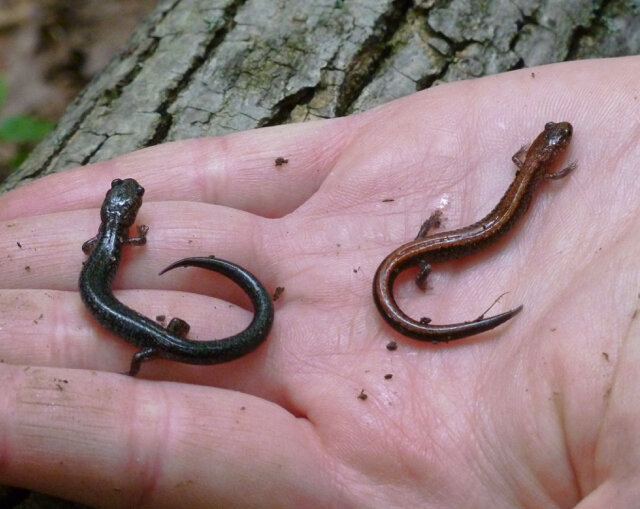
\includegraphics[width=0.5\linewidth]{images/03_plciMorph} 

}

\caption{Unstriped (left) and striped color morphs of red-backed salamanders.}\label{fig:c3f1}
\end{figure}

Let's start by examining an example dataset. A \textbf{dataset} is simply a collection of data, often multiple types. This example dataset is about a phenomenon in wildlife biology called tail autotomy, which refers to the ability of organisms like salamanders and lizards to drop their tail when attacked by a predator. The tail continues to move after it's severed, which is thought to be an adaptation to avoid being eaten. In this case, tail autotomy data was collected for red-backed salamanders (\emph{Plethodon cinereus}), including two different color morphs (striped and unstriped) that are known differ in various behavioral and physiological traits (Figure \ref{fig:c3f1}). The dataset was collected by a former undergraduate student, \href{https://surgery.arizona.edu/person/banan-wael-otaibi-md}{Dr.~Banan Otaibi}, now a surgical resident at the University of Arizona. Dr.~Otaibi's research question was focused on whether tail autotomy behavior differs between color morphs.

\label{tab:c3t1}Dataset on tail autotomy in red-backed salamanders.

individual

morph

tail.sec

tail.vel

mass.g

length.cm

easting

northing

16O300

striped

110

3.0

0.8

3.9

350827

4699989

16O301

striped

160

2.3

0.7

4.0

350827

4699989

16O302

striped

250

2.8

0.9

3.9

350831

4699988

16O303

striped

360

3.3

1.0

4.0

350831

4699988

16O304

striped

220

4.6

0.6

3.4

350831

4699988

16O306

striped

120

3.0

0.6

3.3

352128

4702166

16O308

striped

310

3.5

1.2

4.2

352121

4702172

16O309

striped

220

2.6

0.8

3.7

352122

4702174

16O310

striped

360

2.4

0.7

3.6

352116

4702169

16O311

striped

410

2.6

0.9

3.8

352119

4702170

16O312

striped

190

2.2

1.0

3.8

352110

4702167

16O314

striped

460

2.9

0.8

3.5

352089

4702122

16O315

striped

420

2.2

0.5

3.4

352090

4702135

16O316

striped

440

4.0

0.6

3.3

352088

4702129

16O317

striped

400

3.4

0.9

4.0

352071

4702177

17O300

striped

180

3.5

1.1

4.4

351010

4700176

17O302

striped

270

3.8

0.5

3.2

350989

4700122

17O303

striped

50

1.7

0.6

3.6

350962

4700106

17O304

striped

340

3.2

0.8

4.0

350946

4700091

17O305

striped

300

3.2

1.0

4.1

350939

4700088

16O305

unstriped

10

0.5

0.4

3.1

352130

4702168

16O307

unstriped

0

0.0

0.9

3.6

352119

4702157

16O313

unstriped

20

0.8

0.4

2.9

352090

4702123

16O318

unstriped

10

1.1

0.6

3.3

352075

4702046

17O301

unstriped

70

1.9

0.5

3.3

350990

4700114

17O306

unstriped

70

2.0

0.3

2.8

350910

4700059

17O307

unstriped

10

0.9

0.8

4.2

350910

4700057

17O308

unstriped

30

1.7

0.8

4.0

350887

4700003

17O309

unstriped

50

1.2

1.0

3.9

350889

4699994

17O310

unstriped

50

1.3

0.6

3.4

350893

4700009

17O311

unstriped

0

0.0

0.5

3.5

350855

4699997

17O312

unstriped

0

0.0

0.8

4.0

350871

4700003

17O313

unstriped

50

1.6

0.8

3.9

350838

4700072

17O314

unstriped

20

0.6

0.4

3.0

350982

4700003

17O315

unstriped

20

0.6

0.6

3.4

350957

4699969

17O316

unstriped

50

1.8

0.5

3.5

350795

4699993

17O317

unstriped

50

2.0

0.6

3.6

350789

4700005

17O318

unstriped

40

0.8

0.5

3.4

350811

4700018

17O319

unstriped

50

1.9

0.4

3.1

350806

4700007

17O320

unstriped

80

1.4

0.5

3.3

350812

4700030

\subsection{Variables and observations}\label{variables-and-observations}

The first thing to notice is that the dataset is organized as a table, where each column represents a unique \textbf{variable} and each row represents a unique \textbf{observation} for each observation. A variable is simply a particular type of data, where the observations or measurements can vary. There are eight variables and 40 observations for each variable in the example dataset. Each variable has a unique name. The number of observations for a variable is called the \textbf{sample size}, which is denoted \(n\) or \(N\).

Data are often organized in this tabular format, whether it is in spreadsheet software like Google Sheets or Microsoft Excel, or as we'll see later in this chapter, in statistical software like R. Other names for this tabular format include a \textbf{data matrix} or \textbf{dataframe}, but they all have the common structure of variables in columns and observations in rows. The observations are also referenced under different names, such as measurements, cases, or individuals.

\subsection{Types of varaibles}\label{types-of-varaibles}

Variables can be distinguished between two general types, each with subtypes:

\begin{enumerate}
\def\labelenumi{\arabic{enumi}.}
\item
  \textbf{\emph{Quantitative variables}} Quantitative variables are defined by the observations taking on a range of numeric values. In fact, a synonymous name for a quantitative variable is a \textbf{numeric}. Some quantitative variables have observations that only take on \textbf{discrete} values, such as the number of amino acids composing a protein. In the example dataset, \texttt{tail.sec}, the number of seconds an automized tail moved, is measured as a discrete variable. Other variables are are measured on a \textbf{continuous} scale down to any number of decimal places. For example, mass (\texttt{mass.g}), length (\texttt{length.cm}), and tail velocity (\texttt{tail.vel}, the maximum observed nnumber of tail osciltions) are continuous variables.

  Sometimes quantitative variables can be measured on a discrete or a contiuous scale. For example, you might notice I said \texttt{tail.sec} is \textbf{measured} as a discrete variable, because the observations are integers. But seconds could of course be measured on a continuous scale (e.g., 3.4 seconds).
\item
  \textbf{\emph{Qualitative variables}} Qualitative variables are defined by the observations being classified into different categories. Indeed, qualitative variables are often referred to as \textbf{categorical}, or \textbf{factor} variables. Like quantitative variables, there are different types of qualitative variables. These subcategories reflect whether or not the categories of a variable have an inherent order. When the categories do not have an order, the variable is called \textbf{nominal}. In the example dataset, color morph (\texttt{morph}) is a nominal variable because the categories, striped and unstriped, do not have an order. Other categorical variables have order, such as the life stages of ticks (larva, nymph, adult). Life stage is an \textbf{ordinal} variable, reflecting the ordering in which individuals move through the different life stages.

  Qualitative variables can also be differentiated by the number of categories making up the variable. Specifically, variables with only two categories are called \textbf{binary} variables. Salamander color morph is a good example of a binary variable because color morph can either be striped or unstriped.

  Sometimes it's hard to classify a variable definitively. For example, consider \texttt{individual} in the example dataset. This is simply an alphanumeric code assigned as a unique id for each individual in the dataset. The last few digits of the code are indeed ordered, but the order isn't meaningful.
\end{enumerate}

\subsection{Relationships between variables}\label{relationships-between-variables}

When we ask research questions about causality, we can generally define two types of variables: the variable (or variables - indeed, many processes are not monocausal) inducing a causal effect, and the variable receiving the effect. In the scientific literature, people refer to these different types of variables with different names, so it's a good idea to become familiar with some of the most common terms.

A variable inducing a causal effect is often referred to as an \textbf{explanatory variable}. For example, we might conduct a study on how different types of medication affect blood pressure. In this case, medication type is the explanatory variable. Another common term people use for an explanatory variable is the \textbf{exposure variable}. Here the idea is that the type of medication an individual is exposed to has a causal effect on blood pressures.

The variable receiving causal effects is often referred to the \textbf{response variable}. In the example on medication and blood pressure, blood pressure is the response variable. Another common term for a response variable is an \textbf{outcome variable}.

I will generally use these terms throughout the book, but note these are not the only terms you'll see in the literature. For example, some people refer to explanatory variables as \textbf{independent variables} and response variables as \textbf{dependent variables}. I'm going to avoid using those terms as I tend to think they're confusing because sometimes there are relationships among explanatory variables (i.e., they are \emph{not} independent).

Also note that research questions about prediction are inherently interested in relationships between variables, with the caveat that those relaitonships may not be causal. The research question on tail autotomy is a good example of that. In that case, color morph is the explanatory variable, and we measured two different response variables, total tail movement time (\texttt{tail.sec}) and initial tail velocity (\texttt{tail.vel}). Color morph may well predict tail autotomy, but that relationship may not be causal. Perhaps there's a common genetic variant that contributes to both color morph and the degree of tail autotomy via physiological pathways. We'll explore examples like this in more detail in the next chapter.

\subsection{Variable naming conventions and metadata}\label{variable-naming-conventions-and-metadata}

It's good practice to use a consistent naming style for your variables. Notice that each of the variables in the example database are made of all lower case letters. Some variable names are made up of multiple words or abbreviations, and in the example dataset those components are separated by a period (\texttt{tail.vel}). Those variables with multiple components do not have spaces because spaces are not handled well in statistical software, particularly code-based software (like R). Other conventions to separate components of a variable name work just fine; for example one could separate different components by an underscore (\texttt{tail\_vel}), or by capitalizing the first letter of a new component (\texttt{tailVel}). The most important thing is to be consistent in your approach.

It's also a good idea to get in the habit of generating metadata to go along with your dataset. Metadata is a description of the dataset, including defintiions of variables, their units of measure, and more. Here's some metadata describing the variables in the example dataset:

\begin{table}
\centering
\caption{\label{tab:c3t2}Variable descriptions for a study of the relationship between tail autotomy behavior and color morphology in red-backed salamanders.}
\centering
\begin{tabular}[t]{l|l}
\hline
Variable & Description\\
\hline
individual & Unique identification code for each individual salamander.\\
\hline
morph & Color morph (striped or unstriped) for each salamander.\\
\hline
tail.sec & Total tail movement time (seconds).\\
\hline
tail.vel & Initial tail movement velocity, measured as the maximum observed oscillations per second.\\
\hline
mass.g & Mass in grams\\
\hline
length.cm & Snout-vent-length in cm\\
\hline
easting & Longitudinal geographic coordinate in UTM zone 18 projection (meters).\\
\hline
northing & Latitudinal geographic coordinate in UTM zone 18 projection (meters).\\
\hline
\end{tabular}
\end{table}

\section{Introduction to R}\label{introduction-to-r}

Statistical software is a means to an end. Ultimately our goal is to do good science, and to do that, we must collect and analyze data. In this book, I use the statistical platform R to conduct analyses and create graphical outputs of data. You can find many types of software to perform basic data analyses commonly taught as part of an introductory statistics course. Some are free, and some are not. Some have a graphical user interface where you can point and click to select analyses (e.g., SPSS, JMP), some are spreadsheet-based (e.g., Excel, Google Sheets), and others are code-based, requiring the user to write their own computer code scripts to perform analyses. R is 100\% free, code-based, and widely used in science. In this appendix, I introduce you to the basic data processing skills needed to use R. This material is really intended for those who have no experience using R before. The idea is to introduce some basic skills that will get you up to speed so that you can follow the code and explanations in the book. If you have previously learned basic data processing in R, you can probably skip this material.

\subsection{Installing R and RStudio}\label{installing-r-and-rstudio}

Whereas R is a code-based engine for data processing and analysis, RStudio is an interface that makes it easy to work in R. One of the main advantages of using RStudio to access R is that it is easy to visualize, execute, and save scripts of R code. So while all of the code in this appendix and throughout the book can be executed directly in R, I strongly encourage working with R via RStudio. Like R, RStudio is free.

If you want to install R and RStudio on your own computer, the first thing you should do is download and install R from \url{https://www.r-project.org/}. Click the ``CRAN'' or ``download R'' link, and then choose any mirror to access a download link for your platform (e.g., macOS, Windows, Linux). Once you have installed R, head over to from \url{https://posit.co/download/rstudio-desktop/} and click the the link to Install RStudio, then follow the instructions.

There are also ways of using R and RStudio via cloud-based platforms. Fore example, many universities have invested in \href{https://posit.cloud}{Posit Cloud} for this functionality. With Posit Cloud, you don't need to install R or RStudio to your hard drive, and R code can be easily shared with others. Although it is often handy to have R and RStudio directly on your hard drive, many courses in research design and statistics access R and RStudio via Posit Cloud, so I wanted to mention it here.

\subsection{The RStudio Interface}\label{the-rstudio-interface}

When initially opened, the RStudio interface includes three sections (Figure \ref{fig:c3c1}). The console pane is on the left side, which is where you work with the R environment by typing in or executing code. For numerical data processing, output of your code will generally be displayed in the console (though not always automatically). Graphical output will be displayed in the output pane on the bottom right when viewing the Plots tab. Other tabs in the bottom right allow one to navigate to files on your hard drive, examine help documents, and more. The section at the top right is the Environment pane, which shows the objects that you have loaded in R. We'll dig in first on how to compose and execute code in the R Console.

\begin{figure}

{\centering 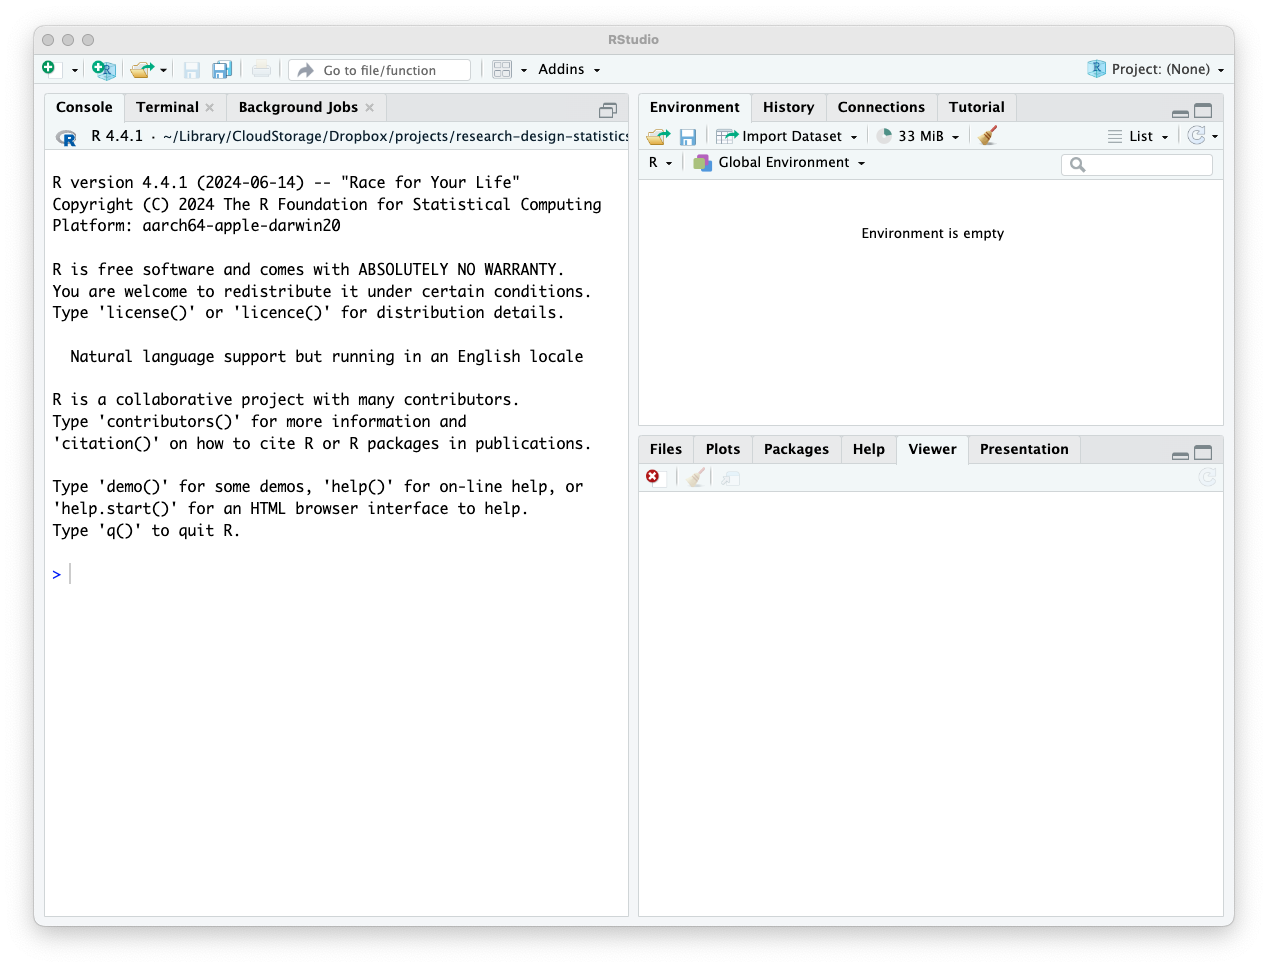
\includegraphics[width=0.8\linewidth]{images/03_rStudio} 

}

\caption{RStudio interface showing the R console (left), working environment (top right), and output (bottom right) panes.}\label{fig:c3c1}
\end{figure}

\subsection{Basic data manipulation in R}\label{basic-data-manipulation-in-r}

\subsubsection{R as a Calculator}\label{r-as-a-calculator}

Let's start simple by using R as a calculator. When you start R, you'll see some background on the version of R you're using and some related information. Below all that you'll see a greater than sign (\texttt{\textgreater{}}). This is the command prompt, and it's where you will type in code that you want to execute. For example, you can do a basic arithmetic such as 2+2 by simply typing in 2+2 and pressing enter.

\begin{Shaded}
\begin{Highlighting}[]
\DecValTok{2}\SpecialCharTok{+}\DecValTok{2}
\end{Highlighting}
\end{Shaded}

\begin{verbatim}
## [1] 4
\end{verbatim}

In the book, I've highlighted R code and like that above in a gray block. Every time I include a chunk of R code, you'll see the command prompt and code to be executed in gray, followed by the output (also in gray), which is the result of the code. So for a simple computation of 2 + 2, you see the command prompt, the 2 + 2 code, and then the output of 4. R prints a number next to the output, here being {[}1{]} for the first line of output.

If you want to include notes in your R code that are not executed as code, all you have to do is add a hash sign (\#) before the text of your note, like this:

\begin{Shaded}
\begin{Highlighting}[]
\DecValTok{2}\SpecialCharTok{+}\DecValTok{2} \CommentTok{\#simple addition}
\end{Highlighting}
\end{Shaded}

\begin{verbatim}
## [1] 4
\end{verbatim}

Here I've added the note \texttt{"simple\ addition"}, which is ignored by R because I included a number side before the text ``simple addition''. See what happens if you don't include the number sign to specify your note:

\begin{Shaded}
\begin{Highlighting}[]
\DecValTok{2}\SpecialCharTok{+}\DecValTok{2}\NormalTok{ simple addition}
\end{Highlighting}
\end{Shaded}

\begin{verbatim}
## Error in parse(text = input): <text>:1:5: unexpected symbol
## 1: 2+2 simple
##         ^
\end{verbatim}

The dreaded red warning text! When output is highlighted in red, that's usually R's way of telling you there's a problem. Here the problem is that R doesn't know what to do with the word ``simple''. There's no number sign signifying ``simple addition'' as a note that should be ignored, so R assumes it's part of your code. Also note that R doesn't even get to ``addition'', it stops executing your code at ``simple'' because it doesn't know how to proceed.

OK, so that's some background on how to execute a simple arithmetic function and include a note. Now go ahead and perform some basic arithmetic computations:

\begin{Shaded}
\begin{Highlighting}[]
\DecValTok{4}\SpecialCharTok{*}\DecValTok{3} \CommentTok{\#simple multiplication}
\end{Highlighting}
\end{Shaded}

\begin{verbatim}
## [1] 12
\end{verbatim}

\begin{Shaded}
\begin{Highlighting}[]
\DecValTok{20}\SpecialCharTok{/}\DecValTok{4} \CommentTok{\#simple division}
\end{Highlighting}
\end{Shaded}

\begin{verbatim}
## [1] 5
\end{verbatim}

\begin{Shaded}
\begin{Highlighting}[]
\FunctionTok{log}\NormalTok{(}\DecValTok{42}\NormalTok{) }\CommentTok{\#the natural log function}
\end{Highlighting}
\end{Shaded}

\begin{verbatim}
## [1] 3.73767
\end{verbatim}

\begin{Shaded}
\begin{Highlighting}[]
\FunctionTok{sqrt}\NormalTok{(}\DecValTok{4}\NormalTok{) }\CommentTok{\#the square root function}
\end{Highlighting}
\end{Shaded}

\begin{verbatim}
## [1] 2
\end{verbatim}

\begin{Shaded}
\begin{Highlighting}[]
\DecValTok{4}\SpecialCharTok{\^{}}\DecValTok{3} \CommentTok{\#raising 4 to the third power}
\end{Highlighting}
\end{Shaded}

\begin{verbatim}
## [1] 64
\end{verbatim}

We're on our way! In the preceding examples, you can see that some text in R is actually meaningful and does not lead to an error. For example, \texttt{log(42)} computes the natural log of 42, and \texttt{sqrt(4)} computes the square root of four. In this case, \texttt{log} and \texttt{sqr}'' are built-in functions in R. More on that soon!

\subsubsection{Objects}\label{objects}

As you can see, it's pretty straightforward to use R as a calculator, but R can do much more. One of the most useful aspects of R is storing data as objects. As a very simple example, suppose we want to assign a value of 4 to a variable that we'll call \texttt{x}:

\begin{Shaded}
\begin{Highlighting}[]
\NormalTok{x }\OtherTok{\textless{}{-}} \DecValTok{4}
\end{Highlighting}
\end{Shaded}

Here we have defined \texttt{x} as 4 with the left arrow, which is a less than sign followed by a dash. The arrow indicates the flow of information, with x on the left being defined as 4. There's nothing special about ``x'' here. For example, I could have defined ``y'' as 4:

\begin{Shaded}
\begin{Highlighting}[]
\NormalTok{y }\OtherTok{\textless{}{-}} \DecValTok{4}
\end{Highlighting}
\end{Shaded}

Or, you can define the object \texttt{Taylor.Swift} as 4:

\begin{Shaded}
\begin{Highlighting}[]
\NormalTok{Taylor.Swift }\OtherTok{\textless{}{-}} \DecValTok{4}
\end{Highlighting}
\end{Shaded}

Note that I didn't include a space between ``Taylor'' and ``Swift''. Try it with a space and see what happens:

\begin{Shaded}
\begin{Highlighting}[]
\NormalTok{Taylor Swift }\OtherTok{\textless{}{-}} \DecValTok{4}
\end{Highlighting}
\end{Shaded}

\begin{verbatim}
## Error in parse(text = input): <text>:1:8: unexpected symbol
## 1: Taylor Swift
##            ^
\end{verbatim}

No good. R doesn't like spaces, so when I define objects that involve more than one word, I usually either include a period or underline between them, or I don't include any characters between them but distinguish components of a variable name by capitalization.

\begin{Shaded}
\begin{Highlighting}[]
\NormalTok{Taylor.Swift }\OtherTok{\textless{}{-}} \DecValTok{4}
\NormalTok{Taylor\_Swift }\OtherTok{\textless{}{-}} \DecValTok{4}
\NormalTok{TaylorSwift }\OtherTok{\textless{}{-}} \DecValTok{4}
\NormalTok{taylorSwift }\OtherTok{\textless{}{-}} \DecValTok{4}
\end{Highlighting}
\end{Shaded}

Notice that R is case sensitive! The objects \texttt{TaylorSwift} and \texttt{taylorSwift} are unique!

OK, great. So I've defined a whole bunch of objects as the value 4. Wait. How do I know each of these objects is 4? Well, type the object name into the R prompt and execute it, and you should see the result is 4:

\begin{Shaded}
\begin{Highlighting}[]
\NormalTok{x}
\end{Highlighting}
\end{Shaded}

\begin{verbatim}
## [1] 4
\end{verbatim}

\begin{Shaded}
\begin{Highlighting}[]
\NormalTok{Taylor.Swift}
\end{Highlighting}
\end{Shaded}

\begin{verbatim}
## [1] 4
\end{verbatim}

Cool! So R will store numeric values - data - symbolically. Quick note: R is case-sensitive. See what happens when you don't capitalize the T and S in \texttt{Taylor.Swift}:

\begin{Shaded}
\begin{Highlighting}[]
\NormalTok{taylor.swift}
\end{Highlighting}
\end{Shaded}

\begin{verbatim}
## Error: object 'taylor.swift' not found
\end{verbatim}

The red text of death. Bummer. This is going to be a major source of frustration as you develop your coding skills. The smallest errors, like a lower-case character when it should be upper-case, will cause your code to fail. If you're hoping to work on your attention to detail, this is going to be a good way to do that!

When we define objects, we can start to use them in functions. For example, what's the square root of \texttt{Taylor.Swift}?

\begin{Shaded}
\begin{Highlighting}[]
\FunctionTok{sqrt}\NormalTok{(Taylor.Swift)}
\end{Highlighting}
\end{Shaded}

\begin{verbatim}
## [1] 2
\end{verbatim}

Clearly it's 2, because \texttt{Taylor.Swift} is 4, and the square root of 4 is 2. How about \texttt{x\ +\ y}?

\begin{Shaded}
\begin{Highlighting}[]
\NormalTok{x }\SpecialCharTok{+}\NormalTok{ y}
\end{Highlighting}
\end{Shaded}

\begin{verbatim}
## [1] 8
\end{verbatim}

Right on - \texttt{x} and \texttt{y} were both defined as 4, so \texttt{x\ +\ y} is 8. Note that we can define these output of these arithmetic functions as new objects:

\begin{Shaded}
\begin{Highlighting}[]
\NormalTok{z }\OtherTok{\textless{}{-}}\NormalTok{ x }\SpecialCharTok{+}\NormalTok{ y}
\NormalTok{z}
\end{Highlighting}
\end{Shaded}

\begin{verbatim}
## [1] 8
\end{verbatim}

Here we defined ``z'' as \texttt{x\ +\ y}, so \texttt{z} is 8. Note that objects can be used to pretty much any degree of complexity:

\begin{Shaded}
\begin{Highlighting}[]
\NormalTok{z}\SpecialCharTok{**}\NormalTok{(x}\SpecialCharTok{+}\NormalTok{y)}\SpecialCharTok{/}\NormalTok{(Taylor.Swift }\SpecialCharTok{{-}}\NormalTok{ x}\SpecialCharTok{**}\NormalTok{y}\SpecialCharTok{*}\NormalTok{z)}
\end{Highlighting}
\end{Shaded}

\begin{verbatim}
## [1] -8208.031
\end{verbatim}

Finally, objects don't have to be numbers. There are different types of objects in R. All of the objects we just defined are called numeric, because they are just numbers. We can also define objects as characters, which are simply strings of text and defined by quotation marks:

\begin{Shaded}
\begin{Highlighting}[]
\SpecialCharTok{\textgreater{}} \DocumentationTok{\#\# Character objects have quotation marks}
\ErrorTok{\textgreater{}}\NormalTok{ singer }\OtherTok{\textless{}{-}} \StringTok{"Taylor Swift"}
\SpecialCharTok{\textgreater{}}\NormalTok{ singer}
\NormalTok{[}\DecValTok{1}\NormalTok{] }\StringTok{"Taylor Swift"}
\end{Highlighting}
\end{Shaded}

Another type of object that we'll encounter a lot in statistics are factor variables, which are categorical variables. I will describe those later.

\subsubsection{Functions}\label{functions}

R has built-in functions that allow you to quickly perform calculations. We've already seen this, such as when we quantified the square root of 4 with the \texttt{sqrt} function. Remember that functions are usually called in R by specifying the name of the function followed by round brackets that enclose the arguments of the function:

\begin{Shaded}
\begin{Highlighting}[]
\SpecialCharTok{\textgreater{}} \FunctionTok{sqrt}\NormalTok{(}\DecValTok{4}\NormalTok{)}
\NormalTok{[}\DecValTok{1}\NormalTok{] }\DecValTok{2}
\end{Highlighting}
\end{Shaded}

The \texttt{sqrt} function is very simple in that it has a single argument, which is the numerical value for which you want to quantify the square root. Other functions have multiple arguments. For example, suppose you want to round the value of 3.147 to a single decimal place. You can use R's built-in \texttt{round} function to do that, which has two arguments. The first argument is the value \texttt{x} you want to round, and the second argument is the number of digits to round to. When you apply a function with multiple arguments, the arguments are separated by a comma:

\begin{Shaded}
\begin{Highlighting}[]
\SpecialCharTok{\textgreater{}} \FunctionTok{round}\NormalTok{(}\AttributeTok{x =} \FloatTok{3.147}\NormalTok{, }\AttributeTok{digits =} \DecValTok{1}\NormalTok{)}
\NormalTok{[}\DecValTok{1}\NormalTok{] }\FloatTok{3.1}
\end{Highlighting}
\end{Shaded}

How did I know which arguments are included in the \texttt{round} function? Built-in functions have supporting documentation that you can read to learn about the function and its arguments. To read the documentation, simply add a question mark in front of the function name, and execute that code:

\begin{Shaded}
\begin{Highlighting}[]
\NormalTok{?round}
\end{Highlighting}
\end{Shaded}

When you execute the code, the bottom right panel in RStudio will show you the ``Help'' document for the round function. You'll see an ``Arguments'' section, and there you'll see that the round function has two arguments (Figure \ref{fig:c3f3}.

\begin{figure}

{\centering 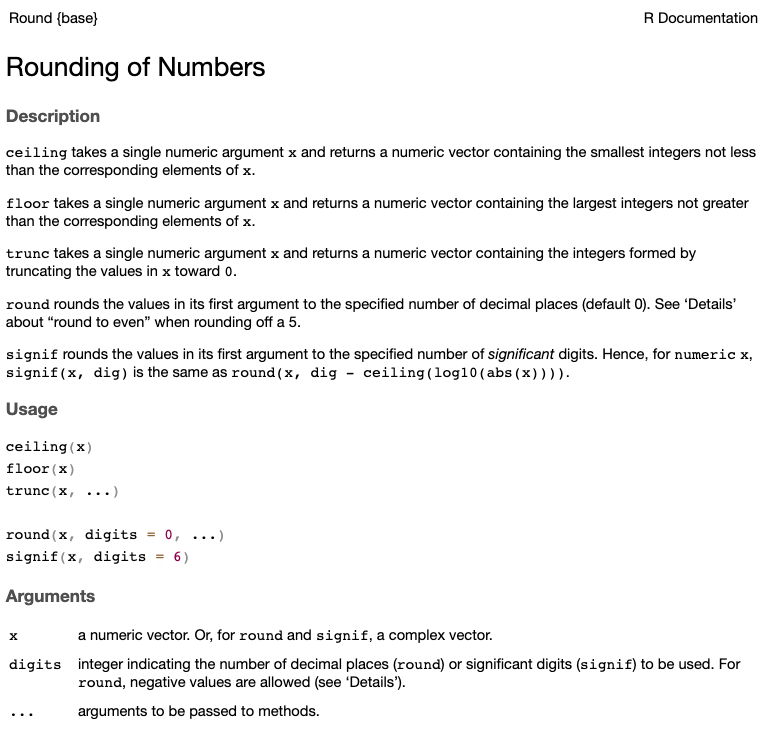
\includegraphics[width=0.8\linewidth]{images/03_documentation} 

}

\caption{Documentation for the round function.}\label{fig:c3f3}
\end{figure}

So we see here that the round function requires a numerical value ``x' to round and the number of''digits'' to round. When you execute code with a function, you can go ahead and use the name of each argument and then specify the value of the argument following an equal sign, like I did above. If you are naming the arguments, the order in which you present the arguments does not matter:

\begin{Shaded}
\begin{Highlighting}[]
\SpecialCharTok{\textgreater{}} \FunctionTok{round}\NormalTok{(}\AttributeTok{x =} \FloatTok{3.147}\NormalTok{, }\AttributeTok{digits =} \DecValTok{1}\NormalTok{)}
\NormalTok{[}\DecValTok{1}\NormalTok{] }\FloatTok{3.1}
\SpecialCharTok{\textgreater{}} \FunctionTok{round}\NormalTok{(}\AttributeTok{digits =} \DecValTok{1}\NormalTok{, }\AttributeTok{x =} \FloatTok{3.147}\NormalTok{)}
\NormalTok{[}\DecValTok{1}\NormalTok{] }\FloatTok{3.1}
\end{Highlighting}
\end{Shaded}

You don't have to name the arguments when executing a function, but there's a catch. When you apply a function and specify the value of the necessary arguments, you have to specify the arguments in the order in which the function expects (x and then digits):

\begin{Shaded}
\begin{Highlighting}[]
\FunctionTok{round}\NormalTok{(}\FloatTok{3.147}\NormalTok{, }\DecValTok{1}\NormalTok{)}
\end{Highlighting}
\end{Shaded}

\begin{verbatim}
## [1] 3.1
\end{verbatim}

If you use the reverse order, you get a different answer:

\begin{Shaded}
\begin{Highlighting}[]
\FunctionTok{round}\NormalTok{(}\DecValTok{1}\NormalTok{, }\FloatTok{3.147}\NormalTok{)}
\end{Highlighting}
\end{Shaded}

\begin{verbatim}
## [1] 1
\end{verbatim}

Note that arguments for a function often have default values. For example, the \texttt{digits} argument in the \texttt{round} function defaults to 0 if not specified, meaning that \texttt{round(3.147)} will round 3.147 to 0 decimal places. The default values can be found in the documentation under the Usage section.

\begin{Shaded}
\begin{Highlighting}[]
\FunctionTok{round}\NormalTok{(}\FloatTok{3.147}\NormalTok{)}
\end{Highlighting}
\end{Shaded}

\begin{verbatim}
## [1] 3
\end{verbatim}

There are many, many functions in R. For example, the function \texttt{class} makes R show what type of object you are dealing with:

\begin{Shaded}
\begin{Highlighting}[]
\SpecialCharTok{\textgreater{}} \FunctionTok{class}\NormalTok{(y)}
\NormalTok{[}\DecValTok{1}\NormalTok{] }\StringTok{"numeric"}
\SpecialCharTok{\textgreater{}} 
\ErrorTok{\textgreater{}} \FunctionTok{class}\NormalTok{(singer)}
\NormalTok{[}\DecValTok{1}\NormalTok{] }\StringTok{"character"}
\end{Highlighting}
\end{Shaded}

\subsubsection{Vectors}\label{vectors}

We know that datasets are made up of one or more variables, each with multiple observations. In R, we can store variables with multiple observations as \textbf{vectors}. For example, suppose we have data on body temperature for five individuals of different ages:

\begin{table}[H]
\centering\centering
\begin{tabular}{r|r}
\hline
\textbf{Age} & \textbf{Temperature (Celcius)}\\
\hline
22 & 98.2\\
\hline
28 & 99.1\\
\hline
34 & 99.3\\
\hline
43 & 98.4\\
\hline
50 & 98.9\\
\hline
\end{tabular}
\end{table}

We can use the concatenate function, \texttt{c}, to create vector for age and temperature:

\begin{Shaded}
\begin{Highlighting}[]
\SpecialCharTok{\textgreater{}} 
\ErrorTok{\textgreater{}} \CommentTok{\# The c() function combines individual values into a single vector}
\ErrorTok{\textgreater{}}\NormalTok{ age }\OtherTok{\textless{}{-}} \FunctionTok{c}\NormalTok{(}\DecValTok{22}\NormalTok{, }\DecValTok{28}\NormalTok{, }\DecValTok{34}\NormalTok{, }\DecValTok{43}\NormalTok{, }\DecValTok{50}\NormalTok{)}
\SpecialCharTok{\textgreater{}}\NormalTok{ age}
\NormalTok{[}\DecValTok{1}\NormalTok{] }\DecValTok{22} \DecValTok{28} \DecValTok{34} \DecValTok{43} \DecValTok{50}
\SpecialCharTok{\textgreater{}} 
\ErrorTok{\textgreater{}} \DocumentationTok{\#\# and now a vector for temperature}
\ErrorTok{\textgreater{}}\NormalTok{ temp }\OtherTok{\textless{}{-}} \FunctionTok{c}\NormalTok{(}\FloatTok{98.2}\NormalTok{, }\FloatTok{99.1}\NormalTok{, }\FloatTok{99.3}\NormalTok{, }\FloatTok{98.4}\NormalTok{, }\FloatTok{98.9}\NormalTok{)}
\SpecialCharTok{\textgreater{}}\NormalTok{ temp}
\NormalTok{[}\DecValTok{1}\NormalTok{] }\FloatTok{98.2} \FloatTok{99.1} \FloatTok{99.3} \FloatTok{98.4} \FloatTok{98.9}
\end{Highlighting}
\end{Shaded}

We can ask R to show us all the values of a vector by simply calling the name of the object, as I've done above. We can also ask R to report particular observations of a vector by using square brackets. For example, to have R report the fifth observation of the temperature vector:

\begin{Shaded}
\begin{Highlighting}[]
\SpecialCharTok{\textgreater{}}\NormalTok{ temp[}\DecValTok{5}\NormalTok{]}
\NormalTok{[}\DecValTok{1}\NormalTok{] }\FloatTok{98.9}
\end{Highlighting}
\end{Shaded}

Note that the temp vector has five observations. What happens if we ask for the sixth observation?

\begin{Shaded}
\begin{Highlighting}[]
\NormalTok{temp[}\DecValTok{6}\NormalTok{]}
\end{Highlighting}
\end{Shaded}

\begin{verbatim}
## [1] NA
\end{verbatim}

Here R reports ``NA'', which means ``not available''. This is simply R's way of telling you that the value you asked for doesn't exist.

If you want to view multiple observations for a vector, you can specify multiple observations with the concatenate function, or you can use a colon to show consecutive observations:

\begin{Shaded}
\begin{Highlighting}[]
\SpecialCharTok{\textgreater{}} 
\ErrorTok{\textgreater{}} \DocumentationTok{\#\# Show the 3rd and 5th observation:}
\ErrorTok{\textgreater{}}\NormalTok{ temp[}\FunctionTok{c}\NormalTok{(}\DecValTok{3}\NormalTok{,}\DecValTok{5}\NormalTok{)]}
\NormalTok{[}\DecValTok{1}\NormalTok{] }\FloatTok{99.3} \FloatTok{98.9}
\SpecialCharTok{\textgreater{}} 
\ErrorTok{\textgreater{}} \DocumentationTok{\#\# Show the 3rd through the 5th observation:}
\ErrorTok{\textgreater{}}\NormalTok{ temp[}\DecValTok{3}\SpecialCharTok{:}\DecValTok{5}\NormalTok{]}
\NormalTok{[}\DecValTok{1}\NormalTok{] }\FloatTok{99.3} \FloatTok{98.4} \FloatTok{98.9}
\end{Highlighting}
\end{Shaded}

If you want to view observations while excluding particular observations, you can do that by adding a minus sign in front of the observation(s) you want to exclude:

\begin{Shaded}
\begin{Highlighting}[]
\SpecialCharTok{\textgreater{}} 
\ErrorTok{\textgreater{}} \DocumentationTok{\#\# Show all but the third observation:}
\ErrorTok{\textgreater{}}\NormalTok{ temp[}\SpecialCharTok{{-}}\DecValTok{3}\NormalTok{]}
\NormalTok{[}\DecValTok{1}\NormalTok{] }\FloatTok{98.2} \FloatTok{99.1} \FloatTok{98.4} \FloatTok{98.9}
\SpecialCharTok{\textgreater{}} 
\ErrorTok{\textgreater{}} \DocumentationTok{\#\# Show all but the third and fifth observation}
\ErrorTok{\textgreater{}}\NormalTok{ temp[}\SpecialCharTok{{-}}\FunctionTok{c}\NormalTok{(}\DecValTok{3}\NormalTok{,}\DecValTok{5}\NormalTok{)]}
\NormalTok{[}\DecValTok{1}\NormalTok{] }\FloatTok{98.2} \FloatTok{99.1} \FloatTok{98.4}
\end{Highlighting}
\end{Shaded}

We can easily apply arithmetic functions to vectors. For example, suppose I wanted to know how many degrees each individual's body temperature is above or below what's considered the ``normal'' value of 98.6 Celcius. Here I'll just ask R to subtract 98.6 from each value in \texttt{temp}, and then save that output as a new object called \texttt{temp.deviation}:

\begin{Shaded}
\begin{Highlighting}[]
\SpecialCharTok{\textgreater{}} 
\ErrorTok{\textgreater{}} 
\ErrorTok{\textgreater{}}\NormalTok{ temp.deviation }\OtherTok{\textless{}{-}}\NormalTok{ temp}\FloatTok{{-}98.6}
\SpecialCharTok{\textgreater{}} 
\ErrorTok{\textgreater{}}\NormalTok{ temp.deviation}
\NormalTok{[}\DecValTok{1}\NormalTok{] }\SpecialCharTok{{-}}\FloatTok{0.4}  \FloatTok{0.5}  \FloatTok{0.7} \SpecialCharTok{{-}}\FloatTok{0.2}  \FloatTok{0.3}
\end{Highlighting}
\end{Shaded}

Here we can see that the first individual's temperature is 0.4 degrees below normal, the second individual is 0.5 degrees above normal, and so forth.

\subsubsection{Matrices}\label{matrices}

Recall that we have body temperature data for individuals of different ages. So far we have created separate vectors for each variable, but each vector has the same structure (5 observations). Remember that datasets of multiple variables are usually organized in a tabular format, with columns representing different variables and rows representing the multiple observations of each variable. In R, we can combine vectors into a single data table called a \textbf{matrix}. Matrices are made of rows and columns, just like a spreadsheet, where the rows represent observations, and the columns represent different objects. Let's make a matrix for our age and temperature data using the \texttt{cbind} function, which combines objects into multiple columns. We'll save this new table and name it \texttt{patient.table}:

\begin{Shaded}
\begin{Highlighting}[]
\SpecialCharTok{\textgreater{}} 
\ErrorTok{\textgreater{}}\NormalTok{ patient.table }\OtherTok{\textless{}{-}} \FunctionTok{cbind}\NormalTok{(age, temp)}
\SpecialCharTok{\textgreater{}} 
\ErrorTok{\textgreater{}}\NormalTok{ patient.table}
\NormalTok{     age temp}
\NormalTok{[}\DecValTok{1}\NormalTok{,]  }\DecValTok{22} \FloatTok{98.2}
\NormalTok{[}\DecValTok{2}\NormalTok{,]  }\DecValTok{28} \FloatTok{99.1}
\NormalTok{[}\DecValTok{3}\NormalTok{,]  }\DecValTok{34} \FloatTok{99.3}
\NormalTok{[}\DecValTok{4}\NormalTok{,]  }\DecValTok{43} \FloatTok{98.4}
\NormalTok{[}\DecValTok{5}\NormalTok{,]  }\DecValTok{50} \FloatTok{98.9}
\end{Highlighting}
\end{Shaded}

We can use square brackets to access observations in a matrix, but now we have to consider that we have two dimensions of data: rows and columns. To extract observations from a matrix, we use a square bracket with row and column values separated by a comma. For example, let's say we want to view the age of the second individual. The second individual is in row 2, and age is the first column in our matrix:

\begin{Shaded}
\begin{Highlighting}[]
\SpecialCharTok{\textgreater{}} 
\ErrorTok{\textgreater{}} \DocumentationTok{\#\# show the age of the second individual}
\ErrorTok{\textgreater{}}\NormalTok{ patient.table[}\DecValTok{2}\NormalTok{,}\DecValTok{1}\NormalTok{]}
\NormalTok{age }
 \DecValTok{28} 
\end{Highlighting}
\end{Shaded}

What if we wanted to view the age AND temperature for the second individual. In this case, we can just leave the column value blank, which R interprets as requesting all the columns:

\begin{Shaded}
\begin{Highlighting}[]
\SpecialCharTok{\textgreater{}} 
\ErrorTok{\textgreater{}} \DocumentationTok{\#\# show all data for the second individual}
\ErrorTok{\textgreater{}}\NormalTok{ patient.table[}\DecValTok{2}\NormalTok{,]}
\NormalTok{ age temp }
\FloatTok{28.0} \FloatTok{99.1} 
\end{Highlighting}
\end{Shaded}

We can also view all the observations for a single variable. Let's say we want to view just the temperature data again. Here we will leave the row value blank but specify the second column for temperature:

\begin{Shaded}
\begin{Highlighting}[]
\SpecialCharTok{\textgreater{}} 
\ErrorTok{\textgreater{}} \DocumentationTok{\#\# show the temperature values}
\ErrorTok{\textgreater{}}\NormalTok{ patient.table[,}\DecValTok{2}\NormalTok{]}
\NormalTok{[}\DecValTok{1}\NormalTok{] }\FloatTok{98.2} \FloatTok{99.1} \FloatTok{99.3} \FloatTok{98.4} \FloatTok{98.9}
\end{Highlighting}
\end{Shaded}

What if we want to add more variables? Let's say we have the body mass index (BMI) for each individual and want to add it to the matrix. We could just create a vector \texttt{bmi}, and then combine it with the other two vectors, or combine it with the \texttt{patient.table} matrix. Either will produce the same output:'

\begin{Shaded}
\begin{Highlighting}[]
\SpecialCharTok{\textgreater{}} 
\ErrorTok{\textgreater{}} \DocumentationTok{\#\# create a bmi vector}
\ErrorTok{\textgreater{}}\NormalTok{ bmi }\OtherTok{\textless{}{-}} \FunctionTok{c}\NormalTok{(}\DecValTok{20}\NormalTok{, }\DecValTok{24}\NormalTok{, }\DecValTok{21}\NormalTok{, }\DecValTok{23}\NormalTok{, }\DecValTok{24}\NormalTok{)}
\SpecialCharTok{\textgreater{}} 
\ErrorTok{\textgreater{}} \DocumentationTok{\#\# combine each vector to create a table}
\ErrorTok{\textgreater{}}\NormalTok{ patient.table.new }\OtherTok{\textless{}{-}} \FunctionTok{cbind}\NormalTok{(age, temp, bmi)}
\SpecialCharTok{\textgreater{}} 
\ErrorTok{\textgreater{}} \DocumentationTok{\#\# or just combine the original table with the new bmi vector}
\ErrorTok{\textgreater{}}\NormalTok{ patient.table }\OtherTok{\textless{}{-}} \FunctionTok{cbind}\NormalTok{(patient.table, bmi)}
\SpecialCharTok{\textgreater{}} 
\ErrorTok{\textgreater{}}\NormalTok{ patient.table}
\NormalTok{     age temp bmi}
\NormalTok{[}\DecValTok{1}\NormalTok{,]  }\DecValTok{22} \FloatTok{98.2}  \DecValTok{20}
\NormalTok{[}\DecValTok{2}\NormalTok{,]  }\DecValTok{28} \FloatTok{99.1}  \DecValTok{24}
\NormalTok{[}\DecValTok{3}\NormalTok{,]  }\DecValTok{34} \FloatTok{99.3}  \DecValTok{21}
\NormalTok{[}\DecValTok{4}\NormalTok{,]  }\DecValTok{43} \FloatTok{98.4}  \DecValTok{23}
\NormalTok{[}\DecValTok{5}\NormalTok{,]  }\DecValTok{50} \FloatTok{98.9}  \DecValTok{24}
\end{Highlighting}
\end{Shaded}

Sometimes we don't have complete data for every variable. In R, remember that missing data are recorded as \texttt{NA} (``Not Available''). For example, suppose we have data on height (inches) for all but the third individual in our dataset. We would specify \texttt{NA} for that individual:

\begin{Shaded}
\begin{Highlighting}[]
\SpecialCharTok{\textgreater{}} 
\ErrorTok{\textgreater{}} \DocumentationTok{\#\# create a height vector}
\ErrorTok{\textgreater{}}\NormalTok{ height }\OtherTok{\textless{}{-}} \FunctionTok{c}\NormalTok{(}\DecValTok{65}\NormalTok{, }\DecValTok{71}\NormalTok{, }\ConstantTok{NA}\NormalTok{, }\DecValTok{68}\NormalTok{, }\DecValTok{66}\NormalTok{)}
\SpecialCharTok{\textgreater{}} 
\ErrorTok{\textgreater{}} \DocumentationTok{\#\# add to the matrix}
\ErrorTok{\textgreater{}}\NormalTok{ patient.table }\OtherTok{\textless{}{-}} \FunctionTok{cbind}\NormalTok{(patient.table, height)}
\SpecialCharTok{\textgreater{}} 
\ErrorTok{\textgreater{}}\NormalTok{ patient.table}
\NormalTok{     age temp bmi height}
\NormalTok{[}\DecValTok{1}\NormalTok{,]  }\DecValTok{22} \FloatTok{98.2}  \DecValTok{20}     \DecValTok{65}
\NormalTok{[}\DecValTok{2}\NormalTok{,]  }\DecValTok{28} \FloatTok{99.1}  \DecValTok{24}     \DecValTok{71}
\NormalTok{[}\DecValTok{3}\NormalTok{,]  }\DecValTok{34} \FloatTok{99.3}  \DecValTok{21}     \ConstantTok{NA}
\NormalTok{[}\DecValTok{4}\NormalTok{,]  }\DecValTok{43} \FloatTok{98.4}  \DecValTok{23}     \DecValTok{68}
\NormalTok{[}\DecValTok{5}\NormalTok{,]  }\DecValTok{50} \FloatTok{98.9}  \DecValTok{24}     \DecValTok{66}
\end{Highlighting}
\end{Shaded}

\subsubsection{Data types in R}\label{data-types-in-r}

Recall that we can generally differentiate variables by their type, either quantitative or qualitative. Each of the four variables we've created so far (\texttt{age}, \texttt{temp}, \texttt{bmi}, \texttt{height}) are quantitative. R defines variable types by their \textbf{class}, and you can ask R to return each object's classification with the \textbf{class} function;

\begin{Shaded}
\begin{Highlighting}[]
\SpecialCharTok{\textgreater{}} 
\ErrorTok{\textgreater{}} \FunctionTok{class}\NormalTok{(age)}
\NormalTok{[}\DecValTok{1}\NormalTok{] }\StringTok{"numeric"}
\SpecialCharTok{\textgreater{}} \FunctionTok{class}\NormalTok{(temp)}
\NormalTok{[}\DecValTok{1}\NormalTok{] }\StringTok{"numeric"}
\SpecialCharTok{\textgreater{}} \FunctionTok{class}\NormalTok{(bmi)}
\NormalTok{[}\DecValTok{1}\NormalTok{] }\StringTok{"numeric"}
\SpecialCharTok{\textgreater{}} \FunctionTok{class}\NormalTok{(height)}
\NormalTok{[}\DecValTok{1}\NormalTok{] }\StringTok{"numeric"}
\end{Highlighting}
\end{Shaded}

We can see R identifies each of these vectors as \textbf{numeric}, which is synonymous with quantitative. Qualitative variables in R are usually classified as \textbf{character} or \textbf{factor} variables. For example, let's create a nominal qualitative variable \textbf{sex}, defining each individual in our dataset as male or female:

\begin{Shaded}
\begin{Highlighting}[]
\DocumentationTok{\#\# create a character for sex}
\NormalTok{sex }\OtherTok{\textless{}{-}} \FunctionTok{c}\NormalTok{(}\StringTok{"female"}\NormalTok{, }\StringTok{"female"}\NormalTok{, }\StringTok{"male"}\NormalTok{, }\StringTok{"female"}\NormalTok{, }\StringTok{"male"}\NormalTok{)}
\FunctionTok{class}\NormalTok{(sex)}
\end{Highlighting}
\end{Shaded}

\begin{verbatim}
## [1] "character"
\end{verbatim}

Notice that \texttt{sex} is classified as a character because the observations consist of text rather than numbers. The other common way of defining and analyzing nominal variables in R is as a factor. We can change the object \texttt{sex} from a character to a factor variable by using the \texttt{as.factor} function:

\begin{Shaded}
\begin{Highlighting}[]
\DocumentationTok{\#\# create a character for sex}
\NormalTok{sex }\OtherTok{\textless{}{-}} \FunctionTok{as.factor}\NormalTok{(sex)}
\FunctionTok{class}\NormalTok{(sex)}
\end{Highlighting}
\end{Shaded}

\begin{verbatim}
## [1] "factor"
\end{verbatim}

When an object is stored as a factor, you can ask R to show you all the levels (i.e., categories) for the variable with the \texttt{levels} function:

\begin{Shaded}
\begin{Highlighting}[]
\FunctionTok{levels}\NormalTok{(sex)}
\end{Highlighting}
\end{Shaded}

\begin{verbatim}
## [1] "female" "male"
\end{verbatim}

Factor variables in R can also consist of levels that are numbers. For example, suppose that we assigned each individual in our dataset to one of three treatments, named ``1'', ``2'', and ``3''. When we initially define the treatment object, R will interpret the class as numeric, but we can change it to a factor:

\begin{Shaded}
\begin{Highlighting}[]
\DocumentationTok{\#\# create treatment variable with numeric codes}
\NormalTok{trt }\OtherTok{\textless{}{-}} \FunctionTok{c}\NormalTok{(}\DecValTok{1}\NormalTok{,}\DecValTok{2}\NormalTok{,}\DecValTok{3}\NormalTok{,}\DecValTok{1}\NormalTok{,}\DecValTok{3}\NormalTok{)}
\FunctionTok{class}\NormalTok{(trt)}
\end{Highlighting}
\end{Shaded}

\begin{verbatim}
## [1] "numeric"
\end{verbatim}

\begin{Shaded}
\begin{Highlighting}[]
\DocumentationTok{\#\# now coerce to factor}
\NormalTok{trt }\OtherTok{\textless{}{-}} \FunctionTok{as.factor}\NormalTok{(trt)}
\FunctionTok{class}\NormalTok{(trt)}
\end{Highlighting}
\end{Shaded}

\begin{verbatim}
## [1] "factor"
\end{verbatim}

\begin{Shaded}
\begin{Highlighting}[]
\FunctionTok{levels}\NormalTok{(trt)}
\end{Highlighting}
\end{Shaded}

\begin{verbatim}
## [1] "1" "2" "3"
\end{verbatim}

When a variable is defined as a factor (or character), functions that treat the variable as numeric will not work. For example, we can't numerically add different factor levels of \texttt{trt}, even though those levels are stored as numbers. R will tell us that mathematical functions applied to factor data doesn't make sense:

\begin{Shaded}
\begin{Highlighting}[]
\NormalTok{trt[}\DecValTok{1}\NormalTok{] }\SpecialCharTok{+}\NormalTok{ trt[}\DecValTok{2}\NormalTok{]}
\end{Highlighting}
\end{Shaded}

\begin{verbatim}
## Warning in Ops.factor(trt[1], trt[2]): '+' not meaningful for factors
\end{verbatim}

\begin{verbatim}
## [1] NA
\end{verbatim}

\subsubsection{Data frames}\label{data-frames}

Remember that datasets are organized in tabular format, as we've seen with a matrix in R. One of hte downsides of using matricies in R is that they are restricted to a single type of data object, for example all numeric or all character objects. If we want to add the nominal variable \texttt{sex} to our data table, we can use a \textbf{data frame}, which are flexible enough to include objects of different class which is a categorical variable made of characters (``male'', ``female''). Here we can use the function \texttt{cbind.data.frame} to combine our matrix of numeric vectors with factor object defining the sex of each individual:

\begin{Shaded}
\begin{Highlighting}[]
\SpecialCharTok{\textgreater{}} 
\ErrorTok{\textgreater{}} \DocumentationTok{\#\# add to the matrix}
\ErrorTok{\textgreater{}}\NormalTok{ patient.table }\OtherTok{\textless{}{-}} \FunctionTok{cbind.data.frame}\NormalTok{(patient.table, sex)}
\SpecialCharTok{\textgreater{}} 
\ErrorTok{\textgreater{}}\NormalTok{ patient.table}
\NormalTok{  age temp bmi height    sex}
\DecValTok{1}  \DecValTok{22} \FloatTok{98.2}  \DecValTok{20}     \DecValTok{65}\NormalTok{ female}
\DecValTok{2}  \DecValTok{28} \FloatTok{99.1}  \DecValTok{24}     \DecValTok{71}\NormalTok{ female}
\DecValTok{3}  \DecValTok{34} \FloatTok{99.3}  \DecValTok{21}     \ConstantTok{NA}\NormalTok{   male}
\DecValTok{4}  \DecValTok{43} \FloatTok{98.4}  \DecValTok{23}     \DecValTok{68}\NormalTok{ female}
\DecValTok{5}  \DecValTok{50} \FloatTok{98.9}  \DecValTok{24}     \DecValTok{66}\NormalTok{   male}
\end{Highlighting}
\end{Shaded}

There are some useful functions to inspect the data frame. For example, if we want to see a list of variables in the data frame, their class, and the first few observations, use the \texttt{str} function. You can see R reports that we have five variables, including four numeric and one factor, and it reports the name of each variable and the first five observations.

\begin{Shaded}
\begin{Highlighting}[]
\SpecialCharTok{\textgreater{}} 
\ErrorTok{\textgreater{}} \FunctionTok{str}\NormalTok{(patient.table)}
\StringTok{\textquotesingle{}data.frame\textquotesingle{}}\SpecialCharTok{:}   \DecValTok{5}\NormalTok{ obs. of  }\DecValTok{5}\NormalTok{ variables}\SpecialCharTok{:}
 \ErrorTok{$}\NormalTok{ age   }\SpecialCharTok{:}\NormalTok{ num  }\DecValTok{22} \DecValTok{28} \DecValTok{34} \DecValTok{43} \DecValTok{50}
 \SpecialCharTok{$}\NormalTok{ temp  }\SpecialCharTok{:}\NormalTok{ num  }\FloatTok{98.2} \FloatTok{99.1} \FloatTok{99.3} \FloatTok{98.4} \FloatTok{98.9}
 \SpecialCharTok{$}\NormalTok{ bmi   }\SpecialCharTok{:}\NormalTok{ num  }\DecValTok{20} \DecValTok{24} \DecValTok{21} \DecValTok{23} \DecValTok{24}
 \SpecialCharTok{$}\NormalTok{ height}\SpecialCharTok{:}\NormalTok{ num  }\DecValTok{65} \DecValTok{71} \ConstantTok{NA} \DecValTok{68} \DecValTok{66}
 \SpecialCharTok{$}\NormalTok{ sex   }\SpecialCharTok{:}\NormalTok{ Factor w}\SpecialCharTok{/} \DecValTok{2}\NormalTok{ levels }\StringTok{"female"}\NormalTok{,}\StringTok{"male"}\SpecialCharTok{:} \DecValTok{1} \DecValTok{1} \DecValTok{2} \DecValTok{1} \DecValTok{2}
\end{Highlighting}
\end{Shaded}

If you just want to see the first few observations in tabular format, use the \texttt{head} function:

\begin{Shaded}
\begin{Highlighting}[]
\SpecialCharTok{\textgreater{}} 
\ErrorTok{\textgreater{}} \FunctionTok{head}\NormalTok{(patient.table)}
\NormalTok{  age temp bmi height    sex}
\DecValTok{1}  \DecValTok{22} \FloatTok{98.2}  \DecValTok{20}     \DecValTok{65}\NormalTok{ female}
\DecValTok{2}  \DecValTok{28} \FloatTok{99.1}  \DecValTok{24}     \DecValTok{71}\NormalTok{ female}
\DecValTok{3}  \DecValTok{34} \FloatTok{99.3}  \DecValTok{21}     \ConstantTok{NA}\NormalTok{   male}
\DecValTok{4}  \DecValTok{43} \FloatTok{98.4}  \DecValTok{23}     \DecValTok{68}\NormalTok{ female}
\DecValTok{5}  \DecValTok{50} \FloatTok{98.9}  \DecValTok{24}     \DecValTok{66}\NormalTok{   male}
\end{Highlighting}
\end{Shaded}

One of nicest things about data frames is that we can call particular objects from the data frame by using their names. This is done by using the dollar sign, \texttt{\$}. For example, if we want to view the observations of height, specify the name of the data frame, then a dollar sign, then the variable name:

\begin{Shaded}
\begin{Highlighting}[]
\SpecialCharTok{\textgreater{}} 
\ErrorTok{\textgreater{}}\NormalTok{ patient.table}\SpecialCharTok{$}\NormalTok{height}
\NormalTok{[}\DecValTok{1}\NormalTok{] }\DecValTok{65} \DecValTok{71} \ConstantTok{NA} \DecValTok{68} \DecValTok{66}
\end{Highlighting}
\end{Shaded}

Note this is the same as calling the fourth column in a matrix as we did before, just more user friendly:

\begin{Shaded}
\begin{Highlighting}[]
\SpecialCharTok{\textgreater{}} 
\ErrorTok{\textgreater{}}\NormalTok{ patient.table[,}\DecValTok{4}\NormalTok{]}
\NormalTok{[}\DecValTok{1}\NormalTok{] }\DecValTok{65} \DecValTok{71} \ConstantTok{NA} \DecValTok{68} \DecValTok{66}
\end{Highlighting}
\end{Shaded}

We can also use the bracket notation specifying variables by names:

\begin{Shaded}
\begin{Highlighting}[]
\SpecialCharTok{\textgreater{}} 
\ErrorTok{\textgreater{}} \DocumentationTok{\#\# view the values for the variable height}
\ErrorTok{\textgreater{}}\NormalTok{ patient.table[,}\StringTok{"height"}\NormalTok{]}
\NormalTok{[}\DecValTok{1}\NormalTok{] }\DecValTok{65} \DecValTok{71} \ConstantTok{NA} \DecValTok{68} \DecValTok{66}
\SpecialCharTok{\textgreater{}} 
\ErrorTok{\textgreater{}} \DocumentationTok{\#\# view the values for age and height}
\ErrorTok{\textgreater{}}\NormalTok{ patient.table[,}\FunctionTok{c}\NormalTok{(}\StringTok{"age"}\NormalTok{, }\StringTok{"height"}\NormalTok{)]}
\NormalTok{  age height}
\DecValTok{1}  \DecValTok{22}     \DecValTok{65}
\DecValTok{2}  \DecValTok{28}     \DecValTok{71}
\DecValTok{3}  \DecValTok{34}     \ConstantTok{NA}
\DecValTok{4}  \DecValTok{43}     \DecValTok{68}
\DecValTok{5}  \DecValTok{50}     \DecValTok{66}
\end{Highlighting}
\end{Shaded}

We can do anything we did before with matrices, such as extracting a subset of observations, or doing arithmetic:

\begin{Shaded}
\begin{Highlighting}[]
\SpecialCharTok{\textgreater{}} 
\ErrorTok{\textgreater{}} \DocumentationTok{\#\# view the values for age and height for the second through fourth individual}
\ErrorTok{\textgreater{}}\NormalTok{ patient.table[}\DecValTok{2}\SpecialCharTok{:}\DecValTok{4}\NormalTok{,}\FunctionTok{c}\NormalTok{(}\StringTok{"age"}\NormalTok{, }\StringTok{"height"}\NormalTok{)]}
\NormalTok{  age height}
\DecValTok{2}  \DecValTok{28}     \DecValTok{71}
\DecValTok{3}  \DecValTok{34}     \ConstantTok{NA}
\DecValTok{4}  \DecValTok{43}     \DecValTok{68}
\SpecialCharTok{\textgreater{}} 
\ErrorTok{\textgreater{}} \DocumentationTok{\#\# view all the values for each variable for the second individual}
\ErrorTok{\textgreater{}}\NormalTok{ patient.table[}\DecValTok{2}\NormalTok{,]}
\NormalTok{  age temp bmi height    sex}
\DecValTok{2}  \DecValTok{28} \FloatTok{99.1}  \DecValTok{24}     \DecValTok{71}\NormalTok{ female}
\SpecialCharTok{\textgreater{}} 
\ErrorTok{\textgreater{}} \DocumentationTok{\#\# quantify deviations from 98.6 for the temperature values:}
\ErrorTok{\textgreater{}}\NormalTok{ patient.table[,}\StringTok{"temp"}\NormalTok{]}\SpecialCharTok{{-}}\FloatTok{98.6}
\NormalTok{[}\DecValTok{1}\NormalTok{] }\SpecialCharTok{{-}}\FloatTok{0.4}  \FloatTok{0.5}  \FloatTok{0.7} \SpecialCharTok{{-}}\FloatTok{0.2}  \FloatTok{0.3}
\end{Highlighting}
\end{Shaded}

\section{Describing variables in R}\label{describing-variables-in-r}

Now that we have some basic R organization and commands under our belt, let's explore some ways of describing data with a simple dataset in R. Characterizing individual variables or relationships between variables is often called \textbf{descriptive statistics}, in contrast to \textbf{inferential statistics} where we want to use statistical analyses to help draw conclusions about scientific hypotheses. This book is ultimately about inference, but because those inferences are being informed by data, some basic skills in describing data are necessary.

\subsection{Loading data into R}\label{loading-data-into-r}

Let's begin by exploring a dataset from \href{https://www.thesquirrelcensus.com/}{The Squirrel Census}. In 2018 a group of volunteers conducted a survey of eastern gray squirrels (\textbf{Sciurus carolinensis}) in New York City's Central Park. They recorded the location of each squirrel along with several behavioral and morphological measurements for each individual.

To explore the data, the first thing we need to do is load the dataset into R. There are multiple types of files that can be loaded into R. One common file type is the \textbf{comma separated values (CSV)} file. CSV files have data organized in columns separated by commas, with separate rows for each row in a data table. CSV files can be generated with a simple text editor, or even in spreadsheet software like Excel or Google Sheets.

Data files can be loaded directly from your computer's hard drive, or from a website. The \texttt{read.csv} function is used to load data from a CSV file into R. Let's start by loading a CSV of the Squirrel Census dataset the example from a file stored on Github. We'll name the data frame \texttt{sq}.

\begin{Shaded}
\begin{Highlighting}[]
\SpecialCharTok{\textgreater{}} 
\ErrorTok{\textgreater{}}\NormalTok{ sq }\OtherTok{\textless{}{-}} \FunctionTok{read.csv}\NormalTok{(}\StringTok{"data/squirrelCensus.csv"}\NormalTok{)}
\SpecialCharTok{\textgreater{}} 
\end{Highlighting}
\end{Shaded}

What if you wanted to load this file from your hard drive? If you do that, you need to specify the directory in which the file is stored. There's two ways to that. First, you could type out the entire directory and file name. For example, if my \texttt{squirrelCensus.csv} file was stored on the Desktop of my Macbook, I would load the file this way:

\begin{Shaded}
\begin{Highlighting}[]
\SpecialCharTok{\textgreater{}} 
\ErrorTok{\textgreater{}}\NormalTok{ sq }\OtherTok{\textless{}{-}} \FunctionTok{read.csv}\NormalTok{(}\StringTok{"/Users/cosentino/Desktop/squirrelCensus.csv"}\NormalTok{)}
\SpecialCharTok{\textgreater{}} 
\end{Highlighting}
\end{Shaded}

If I was loading the file from the desktop of a PC, I'd do it this way:

\begin{Shaded}
\begin{Highlighting}[]
\SpecialCharTok{\textgreater{}} 
\ErrorTok{\textgreater{}}\NormalTok{ sq }\OtherTok{\textless{}{-}} \FunctionTok{read.csv}\NormalTok{(}\StringTok{"C:}\SpecialCharTok{\textbackslash{}\textbackslash{}}\StringTok{Users}\SpecialCharTok{\textbackslash{}\textbackslash{}}\StringTok{cosentino}\SpecialCharTok{\textbackslash{}\textbackslash{}}\StringTok{Desktop}\SpecialCharTok{\textbackslash{}\textbackslash{}}\StringTok{squirrelCensus.csv.csv"}\NormalTok{)}
\SpecialCharTok{\textgreater{}} 
\end{Highlighting}
\end{Shaded}

Second, you can tell RStudio to set the working directory to a particular location on your hard drive where your file is stored. You can do this with a separate function called \texttt{setwd} with the name of the directory is the argument. Once you set the working directory, then you can load a file from that directory simply by referencing the file name:

\begin{Shaded}
\begin{Highlighting}[]
\SpecialCharTok{\textgreater{}} 
\ErrorTok{\textgreater{}} \DocumentationTok{\#\# set the working directory (note no file name is included here)}
\ErrorTok{\textgreater{}} \FunctionTok{setwd}\NormalTok{(}\StringTok{"/Users/cosentino/Desktop/"}\NormalTok{)}
\SpecialCharTok{\textgreater{}} 
\ErrorTok{\textgreater{}} \DocumentationTok{\#\# now load the file }
\ErrorTok{\textgreater{}}\NormalTok{ sq }\OtherTok{\textless{}{-}}\NormalTok{ (}\StringTok{"squirrelCensus.csv.csv"}\NormalTok{)}
\end{Highlighting}
\end{Shaded}

Another type of data format you could load into R is an \textbf{.RData} file. This type of file is specific to R and has at least one named data object stored directly in the file. One nice aspect of RData files is that they can actually store multiple objects. For example, an RData file could include two different dataframes. This can be handy when working with multiple datasets that are related to each other as part of an analysis. I've generated an RData file that has the \texttt{sq} data frame, which you can load in the following way using the \texttt{load} function:

\begin{Shaded}
\begin{Highlighting}[]
\SpecialCharTok{\textgreater{}} 
\ErrorTok{\textgreater{}} \FunctionTok{load}\NormalTok{(data}\SpecialCharTok{/}\NormalTok{squirrelCensus.RData)}
\NormalTok{Error}\SpecialCharTok{:}\NormalTok{ object }\StringTok{\textquotesingle{}squirrelCensus.RData\textquotesingle{}}\NormalTok{ not found}
\end{Highlighting}
\end{Shaded}

Once you've loaded the RData file in this way, the \texttt{sq} data frame should appear in your working environment.

\subsection{Inspecting the dataset}\label{inspecting-the-dataset}

Once you've loaded a file and named a data frame for it, it's generally a good idea to inspect the structure of a new data frame to confirm that everything loaded properly and as you expect it:

\begin{Shaded}
\begin{Highlighting}[]
\SpecialCharTok{\textgreater{}} 
\ErrorTok{\textgreater{}} \FunctionTok{str}\NormalTok{(sq)}
\StringTok{\textquotesingle{}data.frame\textquotesingle{}}\SpecialCharTok{:}   \DecValTok{3023}\NormalTok{ obs. of  }\DecValTok{29}\NormalTok{ variables}\SpecialCharTok{:}
 \ErrorTok{$}\NormalTok{ x                               }\SpecialCharTok{:}\NormalTok{ num  }\SpecialCharTok{{-}}\DecValTok{74} \SpecialCharTok{{-}}\DecValTok{74} \SpecialCharTok{{-}}\DecValTok{74} \SpecialCharTok{{-}}\DecValTok{74} \SpecialCharTok{{-}}\DecValTok{74}\NormalTok{ ...}
 \SpecialCharTok{$}\NormalTok{ y                               }\SpecialCharTok{:}\NormalTok{ num  }\FloatTok{40.8} \FloatTok{40.8} \FloatTok{40.8} \FloatTok{40.8} \FloatTok{40.8}\NormalTok{ ...}
 \SpecialCharTok{$}\NormalTok{ unique.squirrel.id              }\SpecialCharTok{:}\NormalTok{ chr  }\StringTok{"37F{-}PM{-}1014{-}03"} \StringTok{"21B{-}AM{-}1019{-}04"} \StringTok{"11B{-}PM{-}1014{-}08"} \StringTok{"32E{-}PM{-}1017{-}14"}\NormalTok{ ...}
 \SpecialCharTok{$}\NormalTok{ hectare                         }\SpecialCharTok{:}\NormalTok{ chr  }\StringTok{"37F"} \StringTok{"21B"} \StringTok{"11B"} \StringTok{"32E"}\NormalTok{ ...}
 \SpecialCharTok{$}\NormalTok{ shift                           }\SpecialCharTok{:}\NormalTok{ chr  }\StringTok{"PM"} \StringTok{"AM"} \StringTok{"PM"} \StringTok{"PM"}\NormalTok{ ...}
 \SpecialCharTok{$}\NormalTok{ date                            }\SpecialCharTok{:}\NormalTok{ int  }\DecValTok{10142018} \DecValTok{10192018} \DecValTok{10142018} \DecValTok{10172018} \DecValTok{10172018} \DecValTok{10102018} \DecValTok{10102018} \DecValTok{10082018} \DecValTok{10062018} \DecValTok{10102018}\NormalTok{ ...}
 \SpecialCharTok{$}\NormalTok{ hectare.squirrel.number         }\SpecialCharTok{:}\NormalTok{ int  }\DecValTok{3} \DecValTok{4} \DecValTok{8} \DecValTok{14} \DecValTok{5} \DecValTok{3} \DecValTok{2} \DecValTok{2} \DecValTok{1} \DecValTok{3}\NormalTok{ ...}
 \SpecialCharTok{$}\NormalTok{ age                             }\SpecialCharTok{:}\NormalTok{ chr  }\ConstantTok{NA} \ConstantTok{NA} \ConstantTok{NA} \StringTok{"Adult"}\NormalTok{ ...}
 \SpecialCharTok{$}\NormalTok{ primary.fur.color               }\SpecialCharTok{:}\NormalTok{ chr  }\ConstantTok{NA} \ConstantTok{NA} \StringTok{"Gray"} \StringTok{"Gray"}\NormalTok{ ...}
 \SpecialCharTok{$}\NormalTok{ highlight.fur.color             }\SpecialCharTok{:}\NormalTok{ chr  }\ConstantTok{NA} \ConstantTok{NA} \ConstantTok{NA} \ConstantTok{NA}\NormalTok{ ...}
 \SpecialCharTok{$}\NormalTok{ color.notes                     }\SpecialCharTok{:}\NormalTok{ chr  }\ConstantTok{NA} \ConstantTok{NA} \ConstantTok{NA} \StringTok{"Nothing selected as Primary. Gray selected as Highlights. Made executive adjustments."}\NormalTok{ ...}
 \SpecialCharTok{$}\NormalTok{ location                        }\SpecialCharTok{:}\NormalTok{ chr  }\ConstantTok{NA} \ConstantTok{NA} \StringTok{"Above Ground"} \ConstantTok{NA}\NormalTok{ ...}
 \SpecialCharTok{$}\NormalTok{ above.ground.sighter.measurement}\SpecialCharTok{:}\NormalTok{ chr  }\ConstantTok{NA} \ConstantTok{NA} \StringTok{"10"} \ConstantTok{NA}\NormalTok{ ...}
 \SpecialCharTok{$}\NormalTok{ specific.location               }\SpecialCharTok{:}\NormalTok{ chr  }\ConstantTok{NA} \ConstantTok{NA} \ConstantTok{NA} \ConstantTok{NA}\NormalTok{ ...}
 \SpecialCharTok{$}\NormalTok{ running                         }\SpecialCharTok{:}\NormalTok{ logi  }\ConstantTok{FALSE} \ConstantTok{FALSE} \ConstantTok{FALSE} \ConstantTok{FALSE} \ConstantTok{FALSE} \ConstantTok{FALSE}\NormalTok{ ...}
 \SpecialCharTok{$}\NormalTok{ chasing                         }\SpecialCharTok{:}\NormalTok{ logi  }\ConstantTok{FALSE} \ConstantTok{FALSE} \ConstantTok{TRUE} \ConstantTok{FALSE} \ConstantTok{FALSE} \ConstantTok{FALSE}\NormalTok{ ...}
 \SpecialCharTok{$}\NormalTok{ climbing                        }\SpecialCharTok{:}\NormalTok{ logi  }\ConstantTok{FALSE} \ConstantTok{FALSE} \ConstantTok{FALSE} \ConstantTok{FALSE} \ConstantTok{FALSE} \ConstantTok{FALSE}\NormalTok{ ...}
 \SpecialCharTok{$}\NormalTok{ eating                          }\SpecialCharTok{:}\NormalTok{ logi  }\ConstantTok{FALSE} \ConstantTok{FALSE} \ConstantTok{FALSE} \ConstantTok{TRUE} \ConstantTok{FALSE} \ConstantTok{FALSE}\NormalTok{ ...}
 \SpecialCharTok{$}\NormalTok{ foraging                        }\SpecialCharTok{:}\NormalTok{ logi  }\ConstantTok{FALSE} \ConstantTok{FALSE} \ConstantTok{FALSE} \ConstantTok{TRUE} \ConstantTok{TRUE} \ConstantTok{TRUE}\NormalTok{ ...}
 \SpecialCharTok{$}\NormalTok{ other.activities                }\SpecialCharTok{:}\NormalTok{ chr  }\ConstantTok{NA} \ConstantTok{NA} \ConstantTok{NA} \ConstantTok{NA}\NormalTok{ ...}
 \SpecialCharTok{$}\NormalTok{ kuks                            }\SpecialCharTok{:}\NormalTok{ logi  }\ConstantTok{FALSE} \ConstantTok{FALSE} \ConstantTok{FALSE} \ConstantTok{FALSE} \ConstantTok{FALSE} \ConstantTok{FALSE}\NormalTok{ ...}
 \SpecialCharTok{$}\NormalTok{ quaas                           }\SpecialCharTok{:}\NormalTok{ logi  }\ConstantTok{FALSE} \ConstantTok{FALSE} \ConstantTok{FALSE} \ConstantTok{FALSE} \ConstantTok{FALSE} \ConstantTok{FALSE}\NormalTok{ ...}
 \SpecialCharTok{$}\NormalTok{ moans                           }\SpecialCharTok{:}\NormalTok{ logi  }\ConstantTok{FALSE} \ConstantTok{FALSE} \ConstantTok{FALSE} \ConstantTok{FALSE} \ConstantTok{FALSE} \ConstantTok{FALSE}\NormalTok{ ...}
 \SpecialCharTok{$}\NormalTok{ tail.flags                      }\SpecialCharTok{:}\NormalTok{ logi  }\ConstantTok{FALSE} \ConstantTok{FALSE} \ConstantTok{FALSE} \ConstantTok{FALSE} \ConstantTok{FALSE} \ConstantTok{FALSE}\NormalTok{ ...}
 \SpecialCharTok{$}\NormalTok{ tail.twitches                   }\SpecialCharTok{:}\NormalTok{ logi  }\ConstantTok{FALSE} \ConstantTok{FALSE} \ConstantTok{FALSE} \ConstantTok{FALSE} \ConstantTok{FALSE} \ConstantTok{TRUE}\NormalTok{ ...}
 \SpecialCharTok{$}\NormalTok{ approaches                      }\SpecialCharTok{:}\NormalTok{ logi  }\ConstantTok{FALSE} \ConstantTok{FALSE} \ConstantTok{FALSE} \ConstantTok{FALSE} \ConstantTok{FALSE} \ConstantTok{FALSE}\NormalTok{ ...}
 \SpecialCharTok{$}\NormalTok{ indifferent                     }\SpecialCharTok{:}\NormalTok{ logi  }\ConstantTok{FALSE} \ConstantTok{FALSE} \ConstantTok{FALSE} \ConstantTok{FALSE} \ConstantTok{FALSE} \ConstantTok{TRUE}\NormalTok{ ...}
 \SpecialCharTok{$}\NormalTok{ runs.from                       }\SpecialCharTok{:}\NormalTok{ logi  }\ConstantTok{FALSE} \ConstantTok{FALSE} \ConstantTok{FALSE} \ConstantTok{TRUE} \ConstantTok{FALSE} \ConstantTok{FALSE}\NormalTok{ ...}
 \SpecialCharTok{$}\NormalTok{ other.interactions              }\SpecialCharTok{:}\NormalTok{ chr  }\ConstantTok{NA} \ConstantTok{NA} \ConstantTok{NA} \ConstantTok{NA}\NormalTok{ ...}
\end{Highlighting}
\end{Shaded}

We see there are 3023 squirrel observations and 29 variables. Some of the variables are numeric, such as the geographic coordinates \texttt{x} and \texttt{y}, and others are characters, such as the shift during why the squirrel was observed. We also see some new data classes in this file type. For example, \texttt{date} is defined as an integer (``int''). This is simply a discrete quantitative variable. The difference from a numeric varaible in R is largely inconseuqntial; it's just R's way of differentiating between quantitative variables that do or do not have decimals. We also see some variables classified as logical data (``logi'') These are essentially binary data classified as TRUE or FALSE. Fore example, the logical variable climbing would be TRUE if the squirrel was observed climbing and FALSE if it was not. These variables could easily be converted to character or factor classifications, which would be more typical for the analysis of categorical data.

\subsection{Describing single variables}\label{describing-single-variables}

Describing single variables in isolation is really a simple exercise. What are the possible values the variable could take on, and what is the relatively likelihood of those values? In other words, describing single variables is an exercise in characterizing their \textbf{distribution}. How are the values of the variable distributed? What values are most likely, which values are least likely, and how much variation is there among the values?

\subsection{Describing distributions of qualitative variables}\label{describing-distributions-of-qualitative-variables}

Let's take a look at an example in the Squirrel Census dataset: \textbf{primary.fur.color}. This is simply the color of each squirrel observed, so it's a nominal categorical variable, and we can see R has classified this object as a character. How might we describe this variable? The first thing we should do is look at the different levels of this variable. In other words, what are the categories of primary fur color? For a character object, you can use the \texttt{unique} function to see the unique character values for this variable:

\begin{Shaded}
\begin{Highlighting}[]
\SpecialCharTok{\textgreater{}} 
\ErrorTok{\textgreater{}} \FunctionTok{unique}\NormalTok{(sq}\SpecialCharTok{$}\NormalTok{primary.fur.color)}
\NormalTok{[}\DecValTok{1}\NormalTok{] }\ConstantTok{NA}         \StringTok{"Gray"}     \StringTok{"Cinnamon"} \StringTok{"Black"}   
\end{Highlighting}
\end{Shaded}

Here we can see that fur color was classified as gray, cinnamon, or black. Also note that \texttt{NA} is listed as a fur color. Remember that simply means that the primary fur color is unavailable for some individuals.

How should describe the distribution of squirrel color in this dataset? Describing the distribution of categorical variables is actually pretty straightforward. We can simply count up the number of observations of each category. In R we can do this with the \texttt{table} function.

\begin{Shaded}
\begin{Highlighting}[]
\SpecialCharTok{\textgreater{}} 
\ErrorTok{\textgreater{}} \FunctionTok{table}\NormalTok{(sq}\SpecialCharTok{$}\NormalTok{primary.fur.color, }\AttributeTok{useNA=}\StringTok{"always"}\NormalTok{) }\CommentTok{\#useNA="always" means the NA\textquotesingle{}s will be counted}

\NormalTok{   Black Cinnamon     Gray     }\SpecialCharTok{\textless{}}\ConstantTok{NA}\SpecialCharTok{\textgreater{}} 
     \DecValTok{103}      \DecValTok{392}     \DecValTok{2473}       \DecValTok{55} 
\end{Highlighting}
\end{Shaded}

It appears the most common color of squirrels in Central Park is gray, perhaps not surprising for a species named the eastern gray squirrel! But how meaningful is the value 2473 for the number of gray squirrels? On its own, not very meaningful. Raw counts or frequencies of categorical data are only meaningful in light of the total sample size, or the total number of observations in the dataset. We know 2473 is an impressive number of gray squirrels because that makes up the bulk of the 3023 squirrels in the dataset. But we can be more precise. What we really want to know is how common the gray morph is \textbf{relative} to the other morphs, and to look at that, we can quantify the \textbf{proportion} of squirrels of each color morph. A proportion is calculated as

\[
\hat{p} = \frac{x}{n},
\]

where \(\hat{p}\) is the estimated proportion, \(x\) is the observed number of individuals for the category of interest (often called \textbf{successes}), and \(n\) is the total number of individuals in the dataset. Now we could define \(n\) a couple different ways. We could consider that there were \(n = 3023\) squirrels in total, including those 55 individuals without an observed color morph. If we count those individuals towards the total, the raw proportion of squirrels with a primary fur color of gray in the dataset is

\[
\hat{p}_{\text{gray}} = \frac{2473}{3023} = 0.818,
\]

But maybe are most interested in the proportion of squirrel color morphs relative to each other. In that case, we could ignore the 55 squirrels with missing color data and define the sample size as \(n = 3023 - 55 = 2968\) \footnote{The distinction here matters a lot depending on your goal. Every squirrel has a primary fur color whether it is observed or not, so if your goal is to estimate the proportion of each squirrel color in the broader population of squirrels, you really don't want to include the squirrels with a missing color when quantifying the proportion of each morph. As we will see in later chapters, we are making an important assumption if we just ignore the missing observations, specifically that the color of those squirrels are missing at random (i.e., squirrels of any color are equally likely to have missing color data).}:

\[
\hat{p}_{\text{gray}} = \frac{2473}{2968} = 0.833,
\]

There really aren't that many missing observations relative to the total sample size in this dataset, so the difference between these two versions of proportion gray is minimal. You would see a much bigger difference if there were a lot of missing data.

Proportions are probabilities, so one way of interpreting the outcome here is that, of the squirrels in this dataset, the probability of any one squirrel having a primary fur color of gray is 0.818. Proportions can be converted to percentages by multiplying the proportion by 100. Of the squirrels in this dataset, 81.8\% were classified as having a gray primary fur color.

Now you may wonder what the little hat represents over the \(p\). I don't want to get too deep into the weeds on this because we will cover the general ideas in later chapters. For now, all you need to know is that the hat over the \(p\) is indicating we have an \textbf{estimate} of the proportion of squirrels with a primary fur color of gray. In other words, there is some true proportion of gray squirrels in Central Park, and based on this dataset, 0.833 is an estimate of that proportion. At its root, estimation is ultimately what statistics is all about, and we will take a close look at how know if our estimates are any good in later chapter.

OK, back to basic descriptive statistics. What about the proportion of other primary fur colors? Rather than computing the proportions for each color category by hand, we can ask R to compute the proportions using the \texttt{prop.table} function:

\begin{Shaded}
\begin{Highlighting}[]
\SpecialCharTok{\textgreater{}} 
\ErrorTok{\textgreater{}} \FunctionTok{prop.table}\NormalTok{(}\FunctionTok{table}\NormalTok{(sq}\SpecialCharTok{$}\NormalTok{primary.fur.color)) }\CommentTok{\#no longer considering NA observations}

\NormalTok{    Black  Cinnamon      Gray }
\FloatTok{0.0347035} \FloatTok{0.1320755} \FloatTok{0.8332210} 
\end{Highlighting}
\end{Shaded}

All we did here was wrap the \texttt{table} function of the frequency of each coat color in the \texttt{prop.table} function, and now we can see the entire distribution of primary fur color. The most common coat color in the dataset is gray at 83.33\%, followed by cinnamon at 13.2\%, then black at 3.47\%, In addition to displaying the distribution of categorical data as a table, we could also display the distribution in a bar graph:

\begin{Shaded}
\begin{Highlighting}[]
\FunctionTok{barplot}\NormalTok{(}\FunctionTok{table}\NormalTok{(sq}\SpecialCharTok{$}\NormalTok{primary.fur.color), }
        \AttributeTok{ylim=}\FunctionTok{c}\NormalTok{(}\DecValTok{0}\NormalTok{, }\DecValTok{3000}\NormalTok{),}
        \AttributeTok{names.arg =} \FunctionTok{c}\NormalTok{(}\StringTok{"Black"}\NormalTok{, }\StringTok{"Cinnamon"}\NormalTok{, }\StringTok{"Gray"}\NormalTok{),}
        \AttributeTok{col=}\FunctionTok{c}\NormalTok{(}\StringTok{"black"}\NormalTok{, }\StringTok{"brown"}\NormalTok{, }\StringTok{"gray"}\NormalTok{),}
        \AttributeTok{xlab=}\StringTok{"Primary fur color"}\NormalTok{, }\AttributeTok{ylab=}\StringTok{"Individuals"}\NormalTok{, }
        \AttributeTok{main=}\StringTok{"Squirrel Colors in Central Park"}\NormalTok{)}
\end{Highlighting}
\end{Shaded}

\begin{center}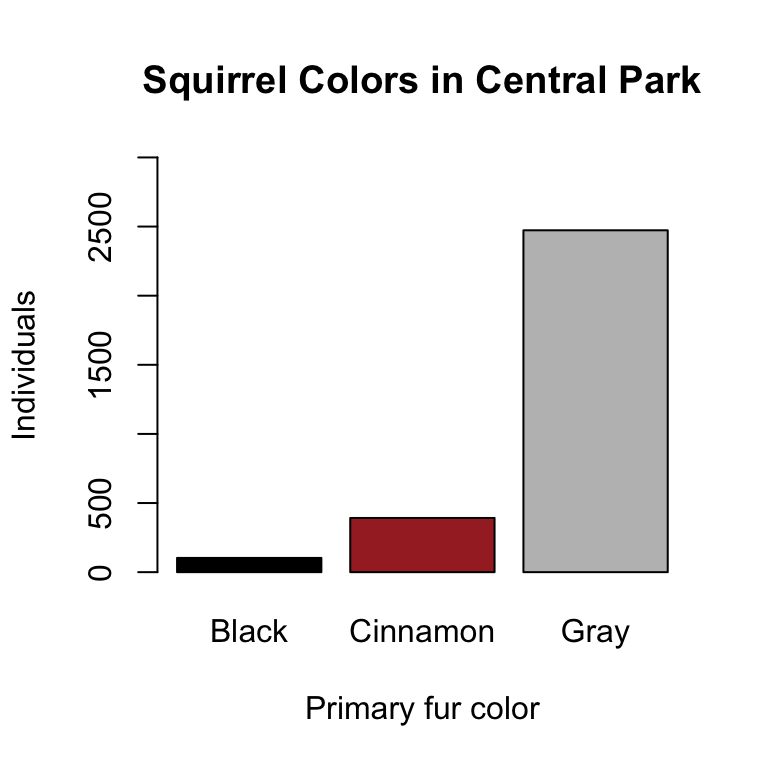
\includegraphics{Research-Design---Statistics_files/figure-latex/c3c66-1} \end{center}

This graph has two axes, the horizontal x-axis and the vertical y-axis. We see the categories of primary fur color on the x-axis and the frequencies of each category on the y-axis. Graphical functions in R aren't all that complex, but the often have a lot of arguments providing the user with options to customize different aspects of the graph. I've specified several arguments in the function:

\begin{itemize}
\tightlist
\item
  \texttt{ylim:} Controls the scale of the y-axis, which I've specified as 0 for the minimum and 3000 for the maximum.\\
\item
  \texttt{names.arg:}: Allows you to specify names for each category, in the same order as the categories are displayed in the output of the \texttt{table} function.
\item
  \texttt{col:} Specifies the color of each bar. These can be all the same, but in this case, I've specified colors that match the descriptions of the primary fur colors.
\item
  \texttt{xlab:} This controls the text for the x-axis label.
\item
  \texttt{ylab:} Text for the y-axis label. and the remaining arguments are used to add axis and plot titles.
\item
  \texttt{main:} Text for the main title of the graph.
\end{itemize}

There are many more arguments you can use to customize figures in R, and I certainly don't have them all memorized. If you want to adjust something, your best bet is to look at the documentation for the plotting function (?barplot in this case) and search for an argument that allows you to do what you want to do!

Note that the bar graph above shows the frequencies of each category of primary fur color, but before I made the point that raw frequences aren't that informative on their own, and that we should generally quantify proportions to characterize the distribution of categorical data. We can easy display the proportions instead of the frequencies, again by wrapping the \texttt{table} function with the \texttt{prop.table} function:

\begin{Shaded}
\begin{Highlighting}[]
\FunctionTok{barplot}\NormalTok{(}\FunctionTok{prop.table}\NormalTok{(}\FunctionTok{table}\NormalTok{(sq}\SpecialCharTok{$}\NormalTok{primary.fur.color)), }
        \AttributeTok{ylim=}\FunctionTok{c}\NormalTok{(}\DecValTok{0}\NormalTok{, }\DecValTok{1}\NormalTok{),}
        \AttributeTok{names.arg =} \FunctionTok{c}\NormalTok{(}\StringTok{"Black"}\NormalTok{, }\StringTok{"Cinnamon"}\NormalTok{, }\StringTok{"Gray"}\NormalTok{),}
        \AttributeTok{col=}\FunctionTok{c}\NormalTok{(}\StringTok{"black"}\NormalTok{, }\StringTok{"brown"}\NormalTok{, }\StringTok{"gray"}\NormalTok{),}
        \AttributeTok{xlab=}\StringTok{"Primary fur color"}\NormalTok{, }\AttributeTok{ylab=}\StringTok{"Proportion"}\NormalTok{, }
        \AttributeTok{main=}\StringTok{"Squirrel Colors in Central Park"}\NormalTok{)}
\end{Highlighting}
\end{Shaded}

\begin{center}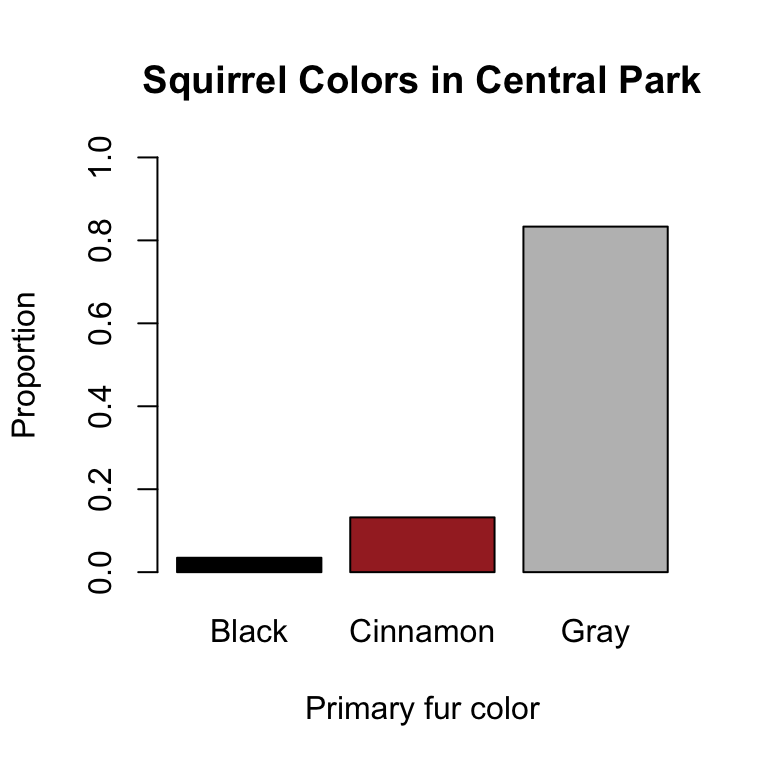
\includegraphics{Research-Design---Statistics_files/figure-latex/c3c67-1} \end{center}

And that's basically it for a basic description of the observed distribution for a categorical variable!

\subsection{Describing distributions of quantitative variables}\label{describing-distributions-of-quantitative-variables}

Let's turn our attention to describing quantitative variables. For this example we'll go back to our dataset on tail autotomy. We start by loading the data and naming the dataframe \texttt{tail} and looking at the structure of the dataframe::

\begin{Shaded}
\begin{Highlighting}[]
\SpecialCharTok{\textgreater{}} 
\ErrorTok{\textgreater{}}\NormalTok{ tail }\OtherTok{\textless{}{-}} \FunctionTok{read.csv}\NormalTok{(}\StringTok{"data/plci\_tails.csv"}\NormalTok{)}
\SpecialCharTok{\textgreater{}} 
\ErrorTok{\textgreater{}} \FunctionTok{str}\NormalTok{(tail)}
\StringTok{\textquotesingle{}data.frame\textquotesingle{}}\SpecialCharTok{:}   \DecValTok{40}\NormalTok{ obs. of  }\DecValTok{8}\NormalTok{ variables}\SpecialCharTok{:}
 \ErrorTok{$}\NormalTok{ individual}\SpecialCharTok{:}\NormalTok{ chr  }\StringTok{"16O300"} \StringTok{"16O301"} \StringTok{"16O302"} \StringTok{"16O303"}\NormalTok{ ...}
 \SpecialCharTok{$}\NormalTok{ morph     }\SpecialCharTok{:}\NormalTok{ chr  }\StringTok{"striped"} \StringTok{"striped"} \StringTok{"striped"} \StringTok{"striped"}\NormalTok{ ...}
 \SpecialCharTok{$}\NormalTok{ tail.sec  }\SpecialCharTok{:}\NormalTok{ int  }\DecValTok{110} \DecValTok{160} \DecValTok{250} \DecValTok{360} \DecValTok{220} \DecValTok{120} \DecValTok{310} \DecValTok{220} \DecValTok{360} \DecValTok{410}\NormalTok{ ...}
 \SpecialCharTok{$}\NormalTok{ tail.vel  }\SpecialCharTok{:}\NormalTok{ num  }\DecValTok{3} \FloatTok{2.3} \FloatTok{2.8} \FloatTok{3.3} \FloatTok{4.6} \DecValTok{3} \FloatTok{3.5} \FloatTok{2.6} \FloatTok{2.4} \FloatTok{2.6}\NormalTok{ ...}
 \SpecialCharTok{$}\NormalTok{ mass.g    }\SpecialCharTok{:}\NormalTok{ num  }\FloatTok{0.8} \FloatTok{0.7} \FloatTok{0.9} \DecValTok{1} \FloatTok{0.6} \FloatTok{0.6} \FloatTok{1.2} \FloatTok{0.8} \FloatTok{0.7} \FloatTok{0.9}\NormalTok{ ...}
 \SpecialCharTok{$}\NormalTok{ length.cm }\SpecialCharTok{:}\NormalTok{ num  }\FloatTok{3.9} \DecValTok{4} \FloatTok{3.9} \DecValTok{4} \FloatTok{3.4} \FloatTok{3.3} \FloatTok{4.2} \FloatTok{3.7} \FloatTok{3.6} \FloatTok{3.8}\NormalTok{ ...}
 \SpecialCharTok{$}\NormalTok{ easting   }\SpecialCharTok{:}\NormalTok{ int  }\DecValTok{350827} \DecValTok{350827} \DecValTok{350831} \DecValTok{350831} \DecValTok{350831} \DecValTok{352128} \DecValTok{352121} \DecValTok{352122} \DecValTok{352116} \DecValTok{352119}\NormalTok{ ...}
 \SpecialCharTok{$}\NormalTok{ northing  }\SpecialCharTok{:}\NormalTok{ int  }\DecValTok{4699989} \DecValTok{4699989} \DecValTok{4699988} \DecValTok{4699988} \DecValTok{4699988} \DecValTok{4702166} \DecValTok{4702172} \DecValTok{4702174} \DecValTok{4702169} \DecValTok{4702170}\NormalTok{ ...}
\end{Highlighting}
\end{Shaded}

Here we see 40 observations of eight variables, as expected. Let's start by examining the distribution of initial tail velocity, which is the number of oscillations of the tail per second after being severed. Characterizing the distribution of a quantitative varible is more involved than for a qualitative variable. When we were describing the primary fur color of squirrels, we could easily compute the proportion of each fur color in the dataset, creating a probability distribution. That was an easy task because categories are discrete units. Quantitative variables, on the other hand, are more tricky because often the data are not discrete. How many salamanders will have an initial velocity of 2.3 oscillations per second? Probably not many! Even if the quantitative variable is discrete (integers), such as tail movement time measured in seconds, there are often very few observations of each particular value.

Let's look at some graphs to show you waht I mean. The distribution of a single quantitative variabe is often displayed as a histogram. Here's an example for the initial tail velocity:

\begin{Shaded}
\begin{Highlighting}[]
\FunctionTok{hist}\NormalTok{(tail}\SpecialCharTok{$}\NormalTok{tail.vel, }
     \AttributeTok{col =} \StringTok{"skyblue"}\NormalTok{,}
     \AttributeTok{main=}\StringTok{""}\NormalTok{,}
     \AttributeTok{xlab=}\StringTok{"Initial velocity (oscillations/sec)"}\NormalTok{, }\AttributeTok{ylab=}\StringTok{"Number of individuals"}\NormalTok{)}
\end{Highlighting}
\end{Shaded}

\begin{center}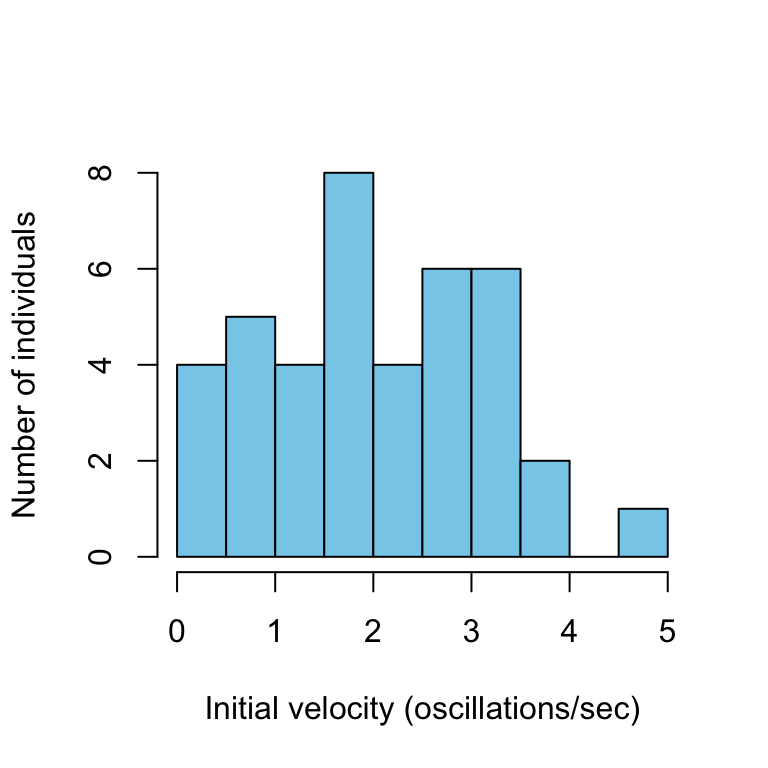
\includegraphics{Research-Design---Statistics_files/figure-latex/c3c69-1} \end{center}

A histogram combines multiple observations that have similar values (x-axis) and shows the frequency of those values (y-axis). The size of the bins in the histogram above are 0.5 oscillations/sec.~For example, we can see there were 4 salamanders with 0-0.5 oscillations/sec, 5 with 0.5-1 oscillations/sec, and so on. The size of the bins is automatically computed with an algorithm, but you could specify the size with the \texttt{breaks} argument. I find the easiest way to specify the breaks is by writing a vector of exactly where I want to breaks. For example, suppose I want breaks every 0.25 units. I can see based on the histogram above that the observations are between 0 and 5, so I want to create breaks every 0.25 units between 0 and 5. I can do this with the \texttt{seq} function. Below are two alternative version of histograms of the same dataset but with bins that are either 0.25 units wide or 0.1 units wide:

\begin{Shaded}
\begin{Highlighting}[]
\FunctionTok{par}\NormalTok{(}\AttributeTok{mfrow=}\FunctionTok{c}\NormalTok{(}\DecValTok{1}\NormalTok{,}\DecValTok{2}\NormalTok{))}
\FunctionTok{hist}\NormalTok{(tail}\SpecialCharTok{$}\NormalTok{tail.vel, }
     \AttributeTok{col =} \StringTok{"skyblue"}\NormalTok{, }\AttributeTok{breaks =} \FunctionTok{seq}\NormalTok{(}\DecValTok{0}\NormalTok{, }\DecValTok{5}\NormalTok{, }\AttributeTok{by =} \FloatTok{0.25}\NormalTok{),}
     \AttributeTok{main =} \StringTok{"Bin size: 0.25 oscillations/sec"}\NormalTok{,}
     \AttributeTok{xlab=}\StringTok{"Initial velocity (oscillations/sec)"}\NormalTok{, }\AttributeTok{ylab=}\StringTok{"Number of individuals"}\NormalTok{)}

\FunctionTok{hist}\NormalTok{(tail}\SpecialCharTok{$}\NormalTok{tail.vel, }
     \AttributeTok{col =} \StringTok{"skyblue"}\NormalTok{, }\AttributeTok{breaks =} \FunctionTok{seq}\NormalTok{(}\DecValTok{0}\NormalTok{, }\DecValTok{5}\NormalTok{, }\AttributeTok{by =} \FloatTok{0.1}\NormalTok{),}
     \AttributeTok{main =} \StringTok{"Bin size: 0.1 oscillations/sec"}\NormalTok{,}
     \AttributeTok{xlab=}\StringTok{"Initial velocity (oscillations/sec)"}\NormalTok{, }\AttributeTok{ylab=}\StringTok{"Number of individuals"}\NormalTok{)}
\end{Highlighting}
\end{Shaded}

\begin{center}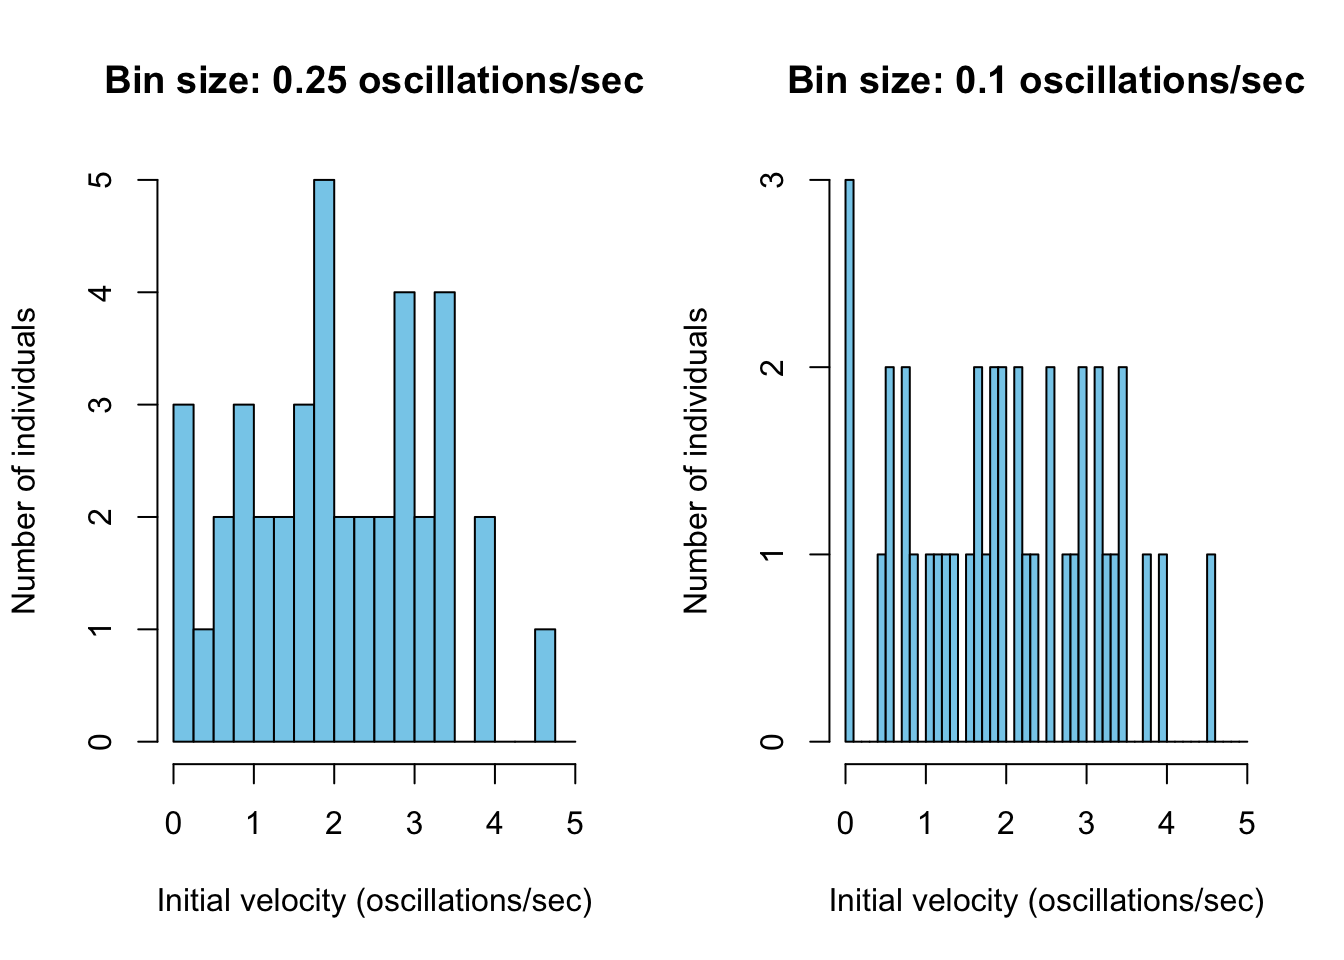
\includegraphics[width=0.85\linewidth]{Research-Design---Statistics_files/figure-latex/c3c70-1} \end{center}

You can see that histograms become less effective for displaying the variation in the data when the bin size gets smaller and smaller, with more observations of 0 salamanders in particular bins. That's a feature of quantitative data. Because numeric variables can be measured to decimal points, there are few observations of any particular value. If the data are measured very precisely and the bin size is smaller than the precision of the data, you'll end up with a histogram showing separate bars for each observation, each with a frequency of a one. That's not helpful. A good rule of thumb is to keep the bin size large enough such that there are few gaps (frequencies of zero) within the range of the observations.

Like qualitative data, it is helpful to characterize the probability distribution of the observations, but again that is made challenging by the fine scale of the observations. What is the probability of initial velocity being 3.213512343243 oscillations/sec? Infinitely small! To resolve this issue, we quantify the \textbf{probability density}, which is the probability that an observation falls within a range of values. Here's the same histogram as our initial histogram, but instead of the y-axis showing frequencies, it now shows probability densities by specifying the \texttt{freq} argument to FALSE:

\begin{Shaded}
\begin{Highlighting}[]
\FunctionTok{hist}\NormalTok{(tail}\SpecialCharTok{$}\NormalTok{tail.vel, }\AttributeTok{freq =} \ConstantTok{FALSE}\NormalTok{,}
     \AttributeTok{col =} \StringTok{"skyblue"}\NormalTok{,}
     \AttributeTok{main=}\StringTok{""}\NormalTok{,}
     \AttributeTok{xlab=}\StringTok{"Initial velocity (oscillations/sec)"}\NormalTok{, }\AttributeTok{ylab=}\StringTok{"Probability density"}\NormalTok{)}
\end{Highlighting}
\end{Shaded}

\begin{center}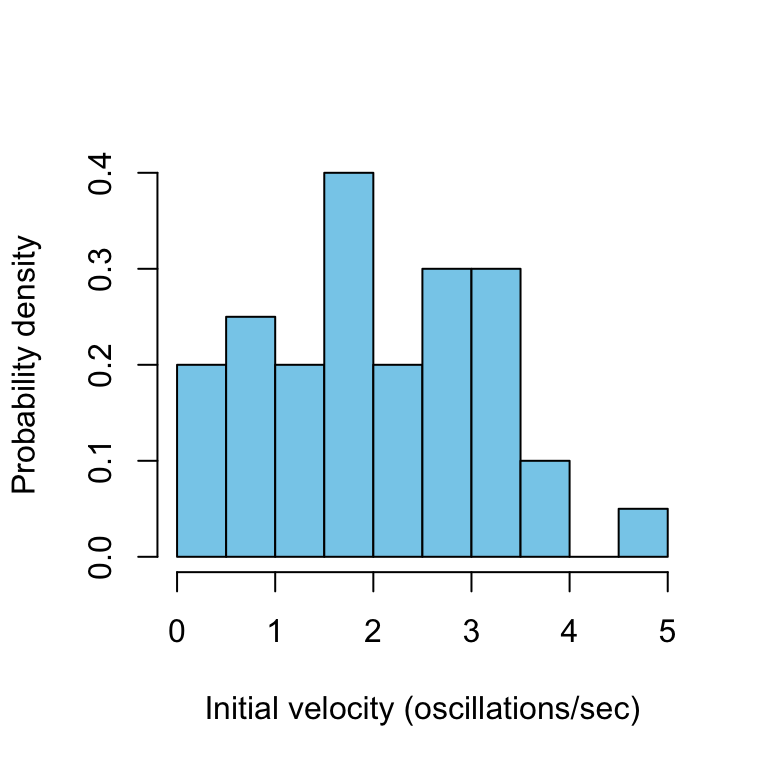
\includegraphics{Research-Design---Statistics_files/figure-latex/c3c71-1} \end{center}

Note that probability \textbf{density} is not the same as a probability. For example, the probability density of initial velocity observations between 1.5 and 2.0 is 0.4. The probability of observations within a particular range, like 1.5 to 2.0 is the area under the probability density curve, in this case \(0.4*0.5 = 0.2\). Indeed 8 out of 40 individuals had an observation between 1.5 and 2, which is 20\%.

Let's crawl out of the weeds a bit. At this point, you basically need to know that characterizing the distribution of a variable requires quantifying the relative probability of different observations, and the way we do that differs between quantitative and qualitative variables.

\subsection{Metrics of central tendency}\label{metrics-of-central-tendency}

Distributions of quantitative variables contain a lot of information, and so it can be helpful to summarize the distributions numerically. One aspect of a distribution is its \textbf{central tendency}. In other words, what are the typical values of a variable? One numeric summary of central tendency is the \textbf{mean}:

\[
\hat{\mu} = \frac{\sum_{i=1}^n x_i}{n},
\]
where \(\hat{\mu}\) is the estimated mean of the variable, \(x_i\) is each observed value of the variable, and \(n\) is the total number of observations. The Greek letter sigma is mathematical notation for summation. The formula basically says to quantify the mean, you need to sum the value of each observation \emph{i} in the dataset, then divide by the total number of observations. The \emph{i} is simply a subscript reprensenting each observation of the variable, from the first (\(i = 1\)) to the last (\(i = n\)). For example, if we have a dataset of \{3, 5, 7, 9, 10\}, the mean is quantified as

\[
\hat{\mu} = \frac{3+5+7+9+10}{5}=6.8
\]

In R, the mean can be quantified with the \texttt{mean} function:

\begin{Shaded}
\begin{Highlighting}[]
\NormalTok{(}\DecValTok{3}\SpecialCharTok{+}\DecValTok{5}\SpecialCharTok{+}\DecValTok{7}\SpecialCharTok{+}\DecValTok{9}\SpecialCharTok{+}\DecValTok{10}\NormalTok{)}\SpecialCharTok{/}\DecValTok{5}
\end{Highlighting}
\end{Shaded}

\begin{verbatim}
## [1] 6.8
\end{verbatim}

\begin{Shaded}
\begin{Highlighting}[]
\FunctionTok{mean}\NormalTok{(}\FunctionTok{c}\NormalTok{(}\DecValTok{3}\NormalTok{,}\DecValTok{5}\NormalTok{,}\DecValTok{7}\NormalTok{,}\DecValTok{9}\NormalTok{,}\DecValTok{10}\NormalTok{))}
\end{Highlighting}
\end{Shaded}

\begin{verbatim}
## [1] 6.8
\end{verbatim}

Let's now go ahead and quantify the mean initial velocity for salamander tails. We can do this by applying the mean function to the variable \texttt{tail.vel} in the tails data frame:

\begin{Shaded}
\begin{Highlighting}[]
\FunctionTok{mean}\NormalTok{(tail}\SpecialCharTok{$}\NormalTok{tail.vel)}
\end{Highlighting}
\end{Shaded}

\begin{verbatim}
## [1] 2.0575
\end{verbatim}

Another common metric of central tendency is the \textbf{median}, which is the middle value of a distribution. Consider again the made-up dataset of \{3, 5, 7, 9, 10\}. The value in the middle is 7, so that's the median. If there's an even number of observations in a dataset, the median can be computed mean of the two middle numbers. For example, if a dataset had observations of \{3, 5, 7, 8, 9, 10\}, the median is the average of 7 and 8: 7.5. The median can be computed with the \texttt{median} function in R. Let's do that for the tail velocity variable:

\begin{Shaded}
\begin{Highlighting}[]
\FunctionTok{median}\NormalTok{(tail}\SpecialCharTok{$}\NormalTok{tail.vel)}
\end{Highlighting}
\end{Shaded}

\begin{verbatim}
## [1] 2
\end{verbatim}

Fascinating. The mean and median tail velocity are very similar, but that's not always the case. Let's quantify the mean and median of the total tail movement time:

\begin{Shaded}
\begin{Highlighting}[]
\FunctionTok{mean}\NormalTok{(tail}\SpecialCharTok{$}\NormalTok{tail.sec)}
\end{Highlighting}
\end{Shaded}

\begin{verbatim}
## [1] 156.25
\end{verbatim}

\begin{Shaded}
\begin{Highlighting}[]
\FunctionTok{median}\NormalTok{(tail}\SpecialCharTok{$}\NormalTok{tail.sec)}
\end{Highlighting}
\end{Shaded}

\begin{verbatim}
## [1] 75
\end{verbatim}

Here we can see the mean of the total tail movement time is 156.25 sec, whereas the median is 75 sec.~That's a huge difference. What gives? It turns out that the similarity of the mean and median depends on the shape of the distribution. Let's compare histograms for tail movement time and tail velocity.

\begin{Shaded}
\begin{Highlighting}[]
\FunctionTok{par}\NormalTok{(}\AttributeTok{mfrow=}\FunctionTok{c}\NormalTok{(}\DecValTok{1}\NormalTok{,}\DecValTok{2}\NormalTok{))}
\FunctionTok{hist}\NormalTok{(tail}\SpecialCharTok{$}\NormalTok{tail.sec,}
     \AttributeTok{col =} \StringTok{"skyblue"}\NormalTok{,}
     \AttributeTok{main=}\StringTok{""}\NormalTok{,}
     \AttributeTok{xlab=}\StringTok{"Total tail movement time (sec)"}\NormalTok{, }\AttributeTok{ylab=}\StringTok{"Individuals"}\NormalTok{)}

\FunctionTok{hist}\NormalTok{(tail}\SpecialCharTok{$}\NormalTok{tail.vel,}
     \AttributeTok{col =} \StringTok{"skyblue"}\NormalTok{,}
     \AttributeTok{main=}\StringTok{""}\NormalTok{,}
     \AttributeTok{xlab=}\StringTok{"Initial velocity (oscillations/sec)"}\NormalTok{, }\AttributeTok{ylab=}\StringTok{"Individuals"}\NormalTok{)}
\end{Highlighting}
\end{Shaded}

\begin{center}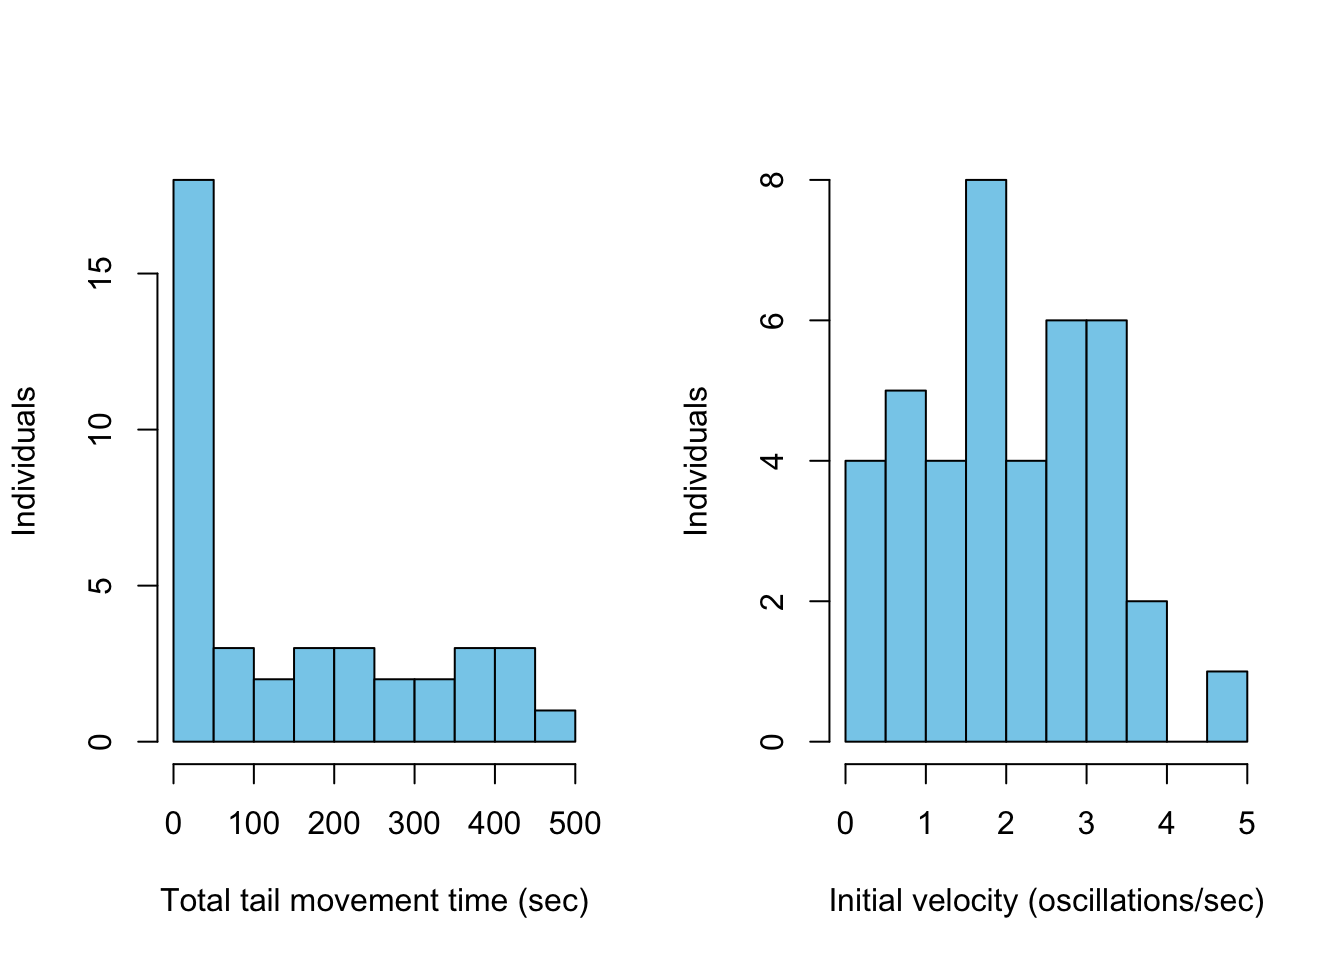
\includegraphics[width=0.85\linewidth]{Research-Design---Statistics_files/figure-latex/c3c76-1} \end{center}

We can see the shape of the two distributions are quite different. The distribution of initial velocity is somewhat bell-shaped, the the majority of observations in the center of the distribution and a minority of observations in both tails of the distribution (i.e., the upper and lower extremes). In contrast, the distribution of total tail movement time is strongly \textbf{skewed}. The most common observations (i.e., the \textbf{mode}) are 0-50 sec, and then there's a long tail of observations to more positive values. There are no observations in the other direction of the mode, which wouldn't make sense because they'd have to be negative. In this case we can describe the distribution as skewed to the riht, or exhibiting positive skew. If the tail extended primarily to more negative values, we can describe the distribution as skewed to the left, or exhibiting negative skew.

\begin{Shaded}
\begin{Highlighting}[]
\FunctionTok{par}\NormalTok{(}\AttributeTok{mfrow=}\FunctionTok{c}\NormalTok{(}\DecValTok{1}\NormalTok{,}\DecValTok{2}\NormalTok{))}
\FunctionTok{hist}\NormalTok{(tail}\SpecialCharTok{$}\NormalTok{tail.vel, }
     \AttributeTok{col =} \StringTok{"skyblue"}\NormalTok{,}
     \AttributeTok{xlab=}\StringTok{"Initial velocity (oscillations/sec)"}\NormalTok{, }\AttributeTok{ylab=}\StringTok{"Number of individuals"}\NormalTok{, }\AttributeTok{main=}\StringTok{""}\NormalTok{)}

\FunctionTok{hist}\NormalTok{(tail}\SpecialCharTok{$}\NormalTok{tail.vel, }\AttributeTok{freq=}\ConstantTok{FALSE}\NormalTok{,}
     \AttributeTok{col =} \StringTok{"skyblue"}\NormalTok{, }
     \AttributeTok{xlab=}\StringTok{"Initial velocity (oscillations/sec)"}\NormalTok{, }\AttributeTok{ylab=}\StringTok{"Probability density"}\NormalTok{, }\AttributeTok{main=}\StringTok{""}\NormalTok{)}
\end{Highlighting}
\end{Shaded}

\begin{center}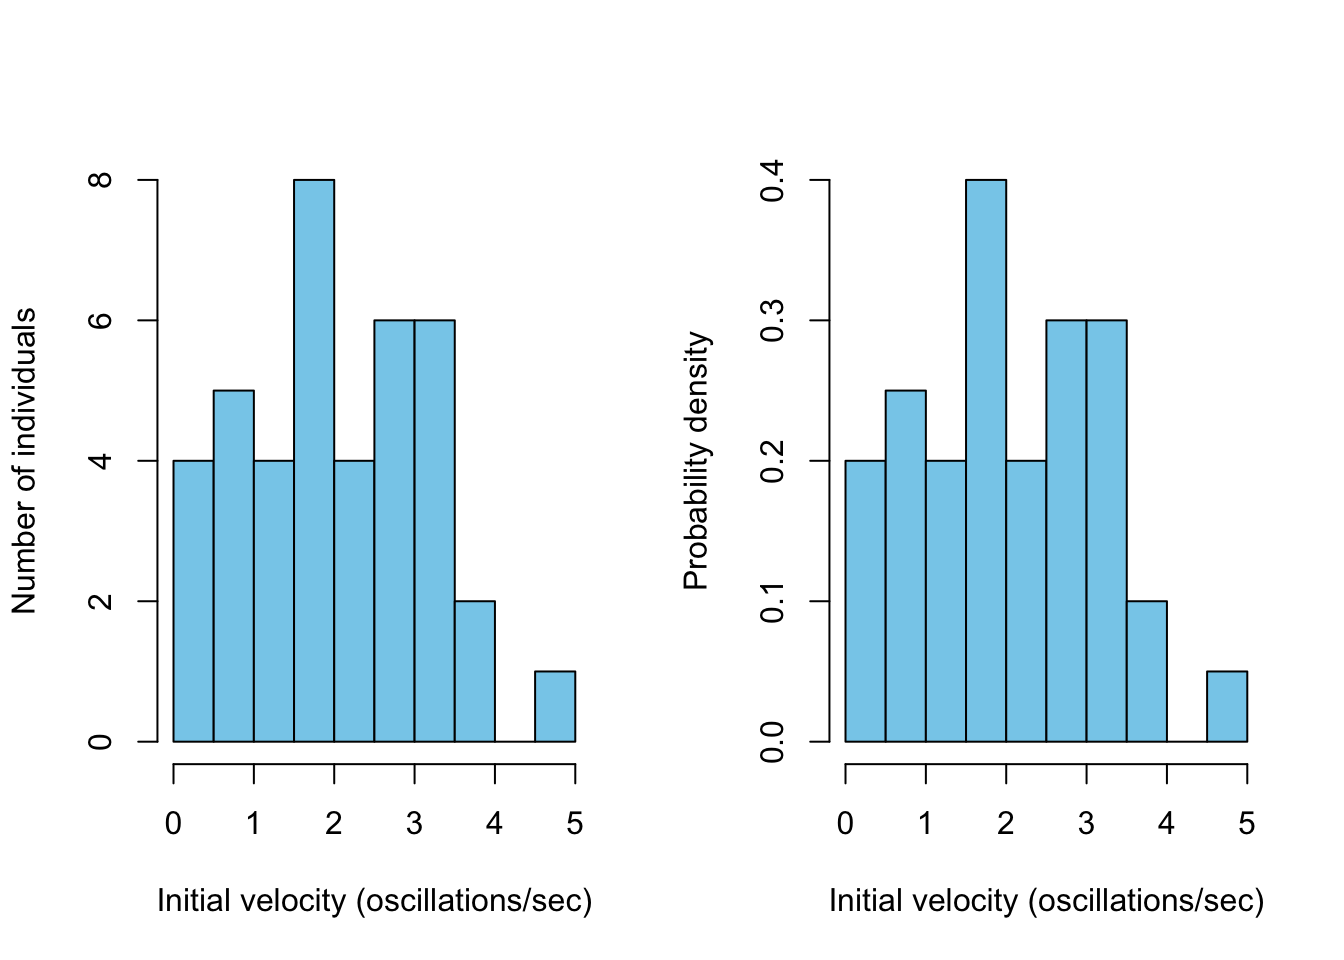
\includegraphics[width=0.85\linewidth]{Research-Design---Statistics_files/figure-latex/c3c77-1} \end{center}

But back to our original point. It turns out the mean and the median are similar to each other for variables with bell-shaped distributions. In fact, if the distribution is perfectly bell-shaped, the mean, median, and mode are all identical. When a variable has a skewed distribution, the mean and median diverge from each other, with the mean being drawn out in the direction of hte skew. The mean is often described as the center of gravity, such that it's sensitive to extreme values. If you change our made-up dataset from \{3, 5, 7, 9, 10\} to \{3, 5, 7, 9, 80\}, the mean changes from 6.8 to 20.8. The median, in contrast, is always the middle observation of the variable. It remains 7 in both datasets.

\subsection{Metrics of variance}\label{metrics-of-variance}

Another way of numerically characterizing a distribution is the variation among observations, which can be quantified with the \textbf{variance}:

\[
\hat{\sigma}^2 = \frac{1}{n-1} \sum_{i=1}^n (x_i - \hat{\mu})^2
\]
Let's take a look at what the variance is doing. We take each observation \(x\), subtract the mean from that value, and then square the term. This value is called a \textbf{squared deviation}, and the variance sums those squared deviations and then divides by the sample size (minus 1). Effectively what's happening here is that the variance is quantifying the mean of the squared deviations from the mean. The more the observations are far away from the mean, the greater the squared deviations, the greater the mean. The variance with our made-up dataset, \{3, 5, 7, 9, 10\}:

\[
\hat{\sigma}^2 = \frac{1}{(5-1)} \left[ (3 - 6.8)^2 + (5 - 6.8)^2 + (7 - 6.8)^2 + (9 - 6.8)^2 + (10 - 6.8)^2 \right] = 8.2
\]
Why is the denominator of the variance \(n-1\) instead of just \(n\)? The quantity \(n-1\) is a bias correction factor when quantifying the variance with a sample of the data. When you only have a subset of observations from the group of interest, the variance tends to be underestimated. More on this in a later chapter when we cover sampling.

In R we can quantify the variance with the \texttt{var} function. Let's apply it to the tail movement and velocity variables:

\begin{Shaded}
\begin{Highlighting}[]
\DocumentationTok{\#\# tail movement time}
\FunctionTok{var}\NormalTok{(tail}\SpecialCharTok{$}\NormalTok{tail.sec)}
\end{Highlighting}
\end{Shaded}

\begin{verbatim}
## [1] 22680.45
\end{verbatim}

\begin{Shaded}
\begin{Highlighting}[]
\DocumentationTok{\#\# initial velocity}
\FunctionTok{var}\NormalTok{(tail}\SpecialCharTok{$}\NormalTok{tail.vel)}
\end{Highlighting}
\end{Shaded}

\begin{verbatim}
## [1] 1.393788
\end{verbatim}

We see the variance in tail movement time is 22680.45 and 1.39 for initial velocity. What are the units? Because we're squaring the deviation of each observation from the mean, the units of variance is the square of the original unit. Thus, the variance of tail movement time is 22680.45 \(sec^2\). Squared units can be difficult to comprehend, but we can put this metric back on the scale of the original units by taking the square root of the variance, which is called the \textbf{standard deviation}:

\[
\hat{\sigma} = \sqrt{\frac{1}{n-1} \sum_{i=1}^n (x_i - \hat{\mu})^2}
\]
The standard deviation can be quantified in R with the \texttt{sd} function:

\begin{Shaded}
\begin{Highlighting}[]
\DocumentationTok{\#\# tail movement time}
\FunctionTok{sd}\NormalTok{(tail}\SpecialCharTok{$}\NormalTok{tail.sec)}
\end{Highlighting}
\end{Shaded}

\begin{verbatim}
## [1] 150.6003
\end{verbatim}

\begin{Shaded}
\begin{Highlighting}[]
\DocumentationTok{\#\# initial velocity}
\FunctionTok{sd}\NormalTok{(tail}\SpecialCharTok{$}\NormalTok{tail.vel)}
\end{Highlighting}
\end{Shaded}

\begin{verbatim}
## [1] 1.180588
\end{verbatim}

We see now that the estimated standard deviation is 150.6 sec for tail movement time and 1.18 oscillations/sec for initial velocity.

\subsection{Percentiles}\label{percentiles}

One last numerical summary of distributions you should be aware of is the \textbf{percentile}, which is defined as the observation in the dataset for which a specified percentage of the data falls below that value. We've actually already seen a percentile. The median is the 50th percentile because 50\% of the observations fall below that value. But you can quantify a percentile for any level of percentage. In R, percentiles are quantified with the \texttt{quantile} function (quantile is a synonymous term for percentile). Here are some percentiles for the tail velocity data:

\begin{Shaded}
\begin{Highlighting}[]
\DocumentationTok{\#\# Report just the 50th percentile (i.e., the median)}
\FunctionTok{quantile}\NormalTok{(tail}\SpecialCharTok{$}\NormalTok{tail.vel, }\AttributeTok{probs =} \FloatTok{0.5}\NormalTok{)}
\end{Highlighting}
\end{Shaded}

\begin{verbatim}
## 50% 
##   2
\end{verbatim}

\begin{Shaded}
\begin{Highlighting}[]
\DocumentationTok{\#\# Report the 0th, 25th, 50th, 75th, and 100th percentiles:}
\FunctionTok{quantile}\NormalTok{(tail}\SpecialCharTok{$}\NormalTok{tail.vel, }\AttributeTok{probs=}\FunctionTok{c}\NormalTok{(}\DecValTok{0}\NormalTok{, }\FloatTok{0.25}\NormalTok{, }\FloatTok{0.5}\NormalTok{, }\FloatTok{0.75}\NormalTok{, }\DecValTok{1}\NormalTok{))}
\end{Highlighting}
\end{Shaded}

\begin{verbatim}
##    0%   25%   50%   75%  100% 
## 0.000 1.175 2.000 3.000 4.600
\end{verbatim}

So we can see that there are no observations below 0, 25\% of the observations are below 1.175, 50\% of the observations are below 2, etc. Note that the 0th and 100th percentiles are the \textbf{minimum} and \textbf{maximum} observations in the data, respectively.

The quantiles are sometimes used to describe variation in the data. Two common metrics are the \textbf{range} and the \textbf{interquartile range (IQR)}. The range is simply the difference between the maximum and minimum observation, whereas the IQR is the difference between the 75th and 25th percentiles. Here are some relevant R functions that you'll find of use:

\begin{Shaded}
\begin{Highlighting}[]
\DocumentationTok{\#\# report the minimum and maximum}
\FunctionTok{range}\NormalTok{(tail}\SpecialCharTok{$}\NormalTok{tail.vel)}
\end{Highlighting}
\end{Shaded}

\begin{verbatim}
## [1] 0.0 4.6
\end{verbatim}

\begin{Shaded}
\begin{Highlighting}[]
\DocumentationTok{\#\# report the range as max {-} min}
\FunctionTok{max}\NormalTok{(tail}\SpecialCharTok{$}\NormalTok{tail.vel) }\SpecialCharTok{{-}} \FunctionTok{min}\NormalTok{(tail}\SpecialCharTok{$}\NormalTok{tail.vel)}
\end{Highlighting}
\end{Shaded}

\begin{verbatim}
## [1] 4.6
\end{verbatim}

\begin{Shaded}
\begin{Highlighting}[]
\DocumentationTok{\#\# IQR}
\FunctionTok{IQR}\NormalTok{(tail}\SpecialCharTok{$}\NormalTok{tail.vel)}
\end{Highlighting}
\end{Shaded}

\begin{verbatim}
## [1] 1.825
\end{verbatim}

\begin{Shaded}
\begin{Highlighting}[]
\DocumentationTok{\#\# IQR calculated with the quantile function}
\FunctionTok{quantile}\NormalTok{(tail}\SpecialCharTok{$}\NormalTok{tail.vel, }\AttributeTok{probs =} \FloatTok{0.75}\NormalTok{) }\SpecialCharTok{{-}} \FunctionTok{quantile}\NormalTok{(tail}\SpecialCharTok{$}\NormalTok{tail.vel, }\AttributeTok{probs =} \FloatTok{0.25}\NormalTok{) }
\end{Highlighting}
\end{Shaded}

\begin{verbatim}
##   75% 
## 1.825
\end{verbatim}

The range is commonly reported for variables to define the bounds of the observed data, but note that the range will be strongly sensitive to extreme observations. For distributions with extreme observations or strong skew, the IQR can be a useful summary statistic to describe variation. Both the range and the IQR have the same units as the original variable.

\subsection{Summary function}\label{summary-function}

The \texttt{summary} function is handy for quickly evaluating the quantiles and mean of a numeric variable. You can apply it to a single vector, or to an entire data frame to summarize all the objects in the data frame at once. If there are characters in the data frame, the \texttt{summary} function will simply indicate that the object is a character of a specific length.

\begin{Shaded}
\begin{Highlighting}[]
\DocumentationTok{\#\# Summary for a single variable}
\FunctionTok{summary}\NormalTok{(tail}\SpecialCharTok{$}\NormalTok{tail.vel)}
\end{Highlighting}
\end{Shaded}

\begin{verbatim}
##    Min. 1st Qu.  Median    Mean 3rd Qu.    Max. 
##   0.000   1.175   2.000   2.058   3.000   4.600
\end{verbatim}

\begin{Shaded}
\begin{Highlighting}[]
\DocumentationTok{\#\# Summary for the entire data frame}
\FunctionTok{summary}\NormalTok{(tail)}
\end{Highlighting}
\end{Shaded}

\begin{verbatim}
##   individual           morph              tail.sec        tail.vel         mass.g      
##  Length:40          Length:40          Min.   :  0.0   Min.   :0.000   Min.   :0.3000  
##  Class :character   Class :character   1st Qu.: 37.5   1st Qu.:1.175   1st Qu.:0.5000  
##  Mode  :character   Mode  :character   Median : 75.0   Median :2.000   Median :0.6500  
##                                        Mean   :156.2   Mean   :2.058   Mean   :0.6975  
##                                        3rd Qu.:277.5   3rd Qu.:3.000   3rd Qu.:0.8250  
##                                        Max.   :460.0   Max.   :4.600   Max.   :1.2000  
##    length.cm        easting          northing      
##  Min.   :2.800   Min.   :350789   Min.   :4699969  
##  1st Qu.:3.300   1st Qu.:350836   1st Qu.:4700003  
##  Median :3.600   Median :350952   Median :4700080  
##  Mean   :3.607   Mean   :351311   Mean   :4700773  
##  3rd Qu.:3.925   3rd Qu.:352089   3rd Qu.:4702130  
##  Max.   :4.400   Max.   :352130   Max.   :4702177
\end{verbatim}

\section{Describing relationships between variables}\label{describing-relationships-between-variables}

Whether your goal is causal explanation or prediction, much of science involves examining relationships between variables. So far we have looked at different ways of describing a single variable. But perhaps the distribution of a variable depends on the value of another variable. We need some basic approaches to describe associations between variables

\subsection{Associations between quantitative variables}\label{associations-between-quantitative-variables}

Does learning something about the length of salamanders tell us anything about their mass? Both length and mass are quantitative variables. The first step to examine the association between two quantitative variables is to create a \textbf{scatterplot}, where each point in the graph displays the values of the two varialbes for each individual in the dataset.

You can create a scatterplot with the \texttt{plot} command in R. The first argument of the plot command asks for the variables. You can either enter the variables separated by a comma (x, y), or you can use a tilde to relate the y to the x variable (y \textasciitilde{} x). Either is fine, but I generally tend to use the tilde format. Note again there are additional arguments to enter x and y axis labels (\texttt{xlab}, \texttt{ylab}), the type of the points (\texttt{pch}), etc. All of the arguments can be viewed with ?plot. Here's the relationship between mass and length:

\begin{Shaded}
\begin{Highlighting}[]
\FunctionTok{plot}\NormalTok{(tail}\SpecialCharTok{$}\NormalTok{mass.g }\SpecialCharTok{\textasciitilde{}}\NormalTok{ tail}\SpecialCharTok{$}\NormalTok{length.cm, }\AttributeTok{asp=}\DecValTok{1}\NormalTok{,}
     \AttributeTok{xlab=}\StringTok{"Snout{-}vent length (cm)"}\NormalTok{, }\AttributeTok{ylab=}\StringTok{"Mass (g)"}\NormalTok{, }\AttributeTok{main=}\StringTok{""}\NormalTok{,}
     \AttributeTok{pch =} \DecValTok{19}\NormalTok{) }\CommentTok{\#pch changes the type of plotting character}
\end{Highlighting}
\end{Shaded}

\begin{center}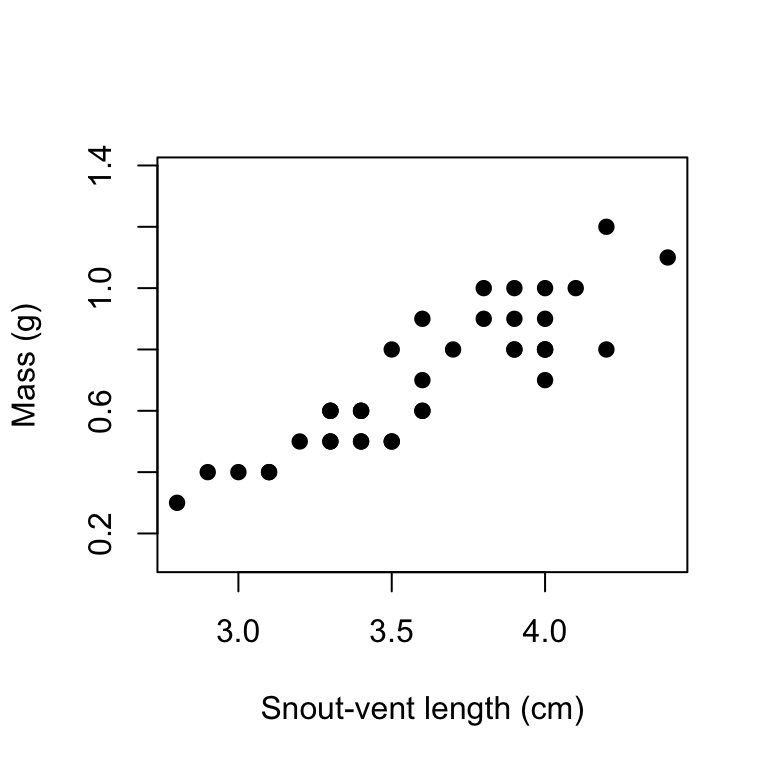
\includegraphics{Research-Design---Statistics_files/figure-latex/c3c83-1} \end{center}

The scatterplot shows a clear pattern. When an individuals length is low, their mass tends to be low as well. When an individual's length is high, their mass tends to be high as well. In other words, there appears to be a positive relationship between mass and length. Scatterplots can also reveal a negative relationships, where the value of one variable tends to decrease as the value of the other variable increases.

The figure below shows a range of possible patterns that one might encounter in scatterplots. Note that in addition to describing the nature of the relationship between variables, we can also describe the magnitude of the relationship. For example, the graph shows two positive relationships in the top row, but the pattern looks much stronger in the scatterplot on the left than the scatterplot on the right.

\begin{center}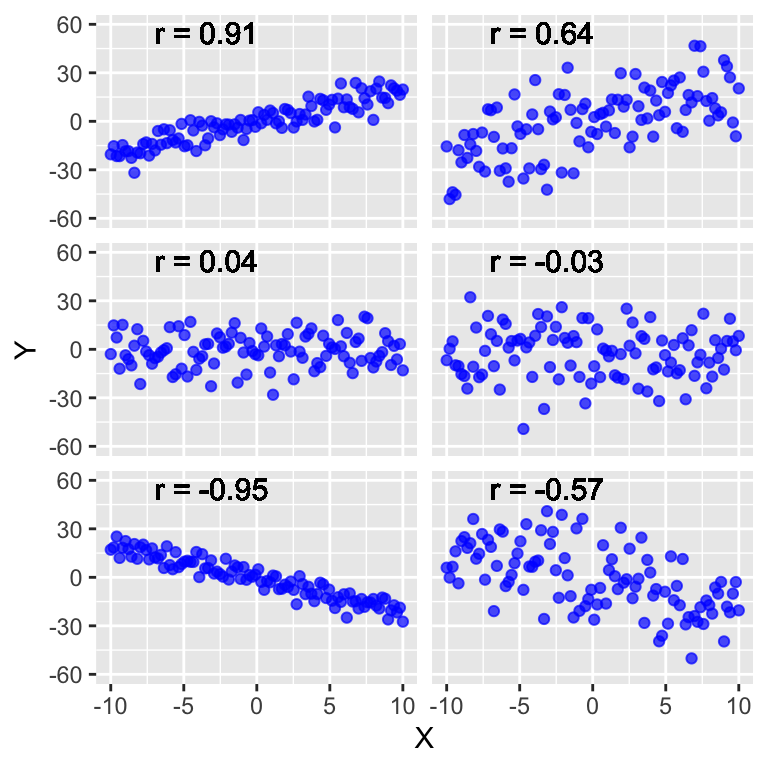
\includegraphics{Research-Design---Statistics_files/figure-latex/c3c84-1} \end{center}

The \textbf{correlation coefficient (r)} is a numerical metric used to describe both the direction and strength of an association. It has a bit of a messy formula:

\[
r = \frac{\frac{1}{n-1} \sum_{i=1}^n (x_i - \hat{\mu}_x)(y_i - \hat{\mu}_y)}{\hat{\sigma}_x \hat{\sigma}_y}
\]
I don't want to get into the mathemeatical details here, but at a very basic level, the correlation coefficient is based on the \textbf{covariance}, which is the numerator in the formula for the correlation coefficient. The covariance is a cross product of the deviation between each value of variables \(x\) and \(y\) from their mean. When \(x\) and \(y\) values have a common relationship to their mean, the covariance is positive. This would reflect a positive association, where high values of \(x\) correspond to high values of \(y\), and vice versa. When \(x\) and \(y\) values have opposite relationship to their mean, the covariance is negative. This would reflect a negative association, where high values of \(x\) correspond to low values of \(y\), and vice versa. When there's no association between \(x\) and \(y\), the covariance is 0. Covariance has awkward units. The correlation coefficint divides the covariance by the standard deviations of each variable, which standardizes the association to be between -1 and 1. Negative values reflect negative associations, positive values reflect positive associations, and \(r=0\) reflects no association. The strength of the association is reflected by how close the value of \(r\) is to 1 or -1. Stronger associations have values of \(r\) close to 1 or -1. You can see this in the example scatterplots, where stronger associations reflect less scatter among the points. When \(r\) is exactly 1 or -1, the points all fall on a perfect line.

Does it matter which variable we place on each axis when examining the association between two quantitative variables? It can. If your goal is causal explanation, you should generally place the explanatory variable on the x-axis and the repsonse variable on the y-axis. The length of an animal is almost certainly one cause of its mass, so it makes sense that we placed length on the x-axis. But don't assume that an association between two variables is causal! When we describe associations between variables, all we are doing is describing patterns. We'll need additional tools to say whether or not the patterns we find in the data reflect some kind of causal process. More on that in later chapters.

\subsection{Associations between quantitative and qualitative variables}\label{associations-between-quantitative-and-qualitative-variables}

Let's look at how to compare quantitative data between categories of a qualitative variable. The idea here is to visually inspect how the distribution of the quantitative variable differs between categories of the qualitative variable. In this section, we'll compare initial velocity of tail movement between the color morphs.

\subsubsection{Making data subsets and plotting by subset}\label{making-data-subsets-and-plotting-by-subset}

One way of comparing quantitative variables by categories is to subset the observations by categories. This requires two steps. First, you need to subset the observations in your dataframe by the levels of the qualitative variable of interest. This can be done in a number of different ways. One way is to use our matrix notation and indexing approach:

\begin{Shaded}
\begin{Highlighting}[]
\CommentTok{\#create a separate dataframe for striped salamanders}
\NormalTok{tail.striped   }\OtherTok{\textless{}{-}}\NormalTok{ tail[tail}\SpecialCharTok{$}\NormalTok{morph }\SpecialCharTok{==} \StringTok{"striped"}\NormalTok{, ]}
\FunctionTok{head}\NormalTok{(tail.striped)}
\end{Highlighting}
\end{Shaded}

\begin{verbatim}
##   individual   morph tail.sec tail.vel mass.g length.cm easting northing
## 1     16O300 striped      110      3.0    0.8       3.9  350827  4699989
## 2     16O301 striped      160      2.3    0.7       4.0  350827  4699989
## 3     16O302 striped      250      2.8    0.9       3.9  350831  4699988
## 4     16O303 striped      360      3.3    1.0       4.0  350831  4699988
## 5     16O304 striped      220      4.6    0.6       3.4  350831  4699988
## 6     16O306 striped      120      3.0    0.6       3.3  352128  4702166
\end{verbatim}

\begin{Shaded}
\begin{Highlighting}[]
\CommentTok{\#create a separate dataframe for unstriped salamanders}
\NormalTok{tail.unstriped }\OtherTok{\textless{}{-}}\NormalTok{ tail[tail}\SpecialCharTok{$}\NormalTok{morph }\SpecialCharTok{==} \StringTok{"unstriped"}\NormalTok{, ]}
\FunctionTok{head}\NormalTok{(tail.unstriped)}
\end{Highlighting}
\end{Shaded}

\begin{verbatim}
##    individual     morph tail.sec tail.vel mass.g length.cm easting northing
## 21     16O305 unstriped       10      0.5    0.4       3.1  352130  4702168
## 22     16O307 unstriped        0      0.0    0.9       3.6  352119  4702157
## 23     16O313 unstriped       20      0.8    0.4       2.9  352090  4702123
## 24     16O318 unstriped       10      1.1    0.6       3.3  352075  4702046
## 25     17O301 unstriped       70      1.9    0.5       3.3  350990  4700114
## 26     17O306 unstriped       70      2.0    0.3       2.8  350910  4700059
\end{verbatim}

Here we have asked R to extract observations in the \texttt{tail} dataframe that meet a condition, namely when \texttt{tail\$morph} is \texttt{striped} or \texttt{unstriped}, and we create new subset dataframes for each morph.

Another way we can create subsets is with the \texttt{subset} function.

\begin{Shaded}
\begin{Highlighting}[]
\CommentTok{\#create a separate dataframe for striped salamanders}
\NormalTok{tail.striped }\OtherTok{\textless{}{-}} \FunctionTok{subset}\NormalTok{(tail, morph }\SpecialCharTok{==} \StringTok{"striped"}\NormalTok{)}
\FunctionTok{head}\NormalTok{(tail.striped)}
\end{Highlighting}
\end{Shaded}

\begin{verbatim}
##   individual   morph tail.sec tail.vel mass.g length.cm easting northing
## 1     16O300 striped      110      3.0    0.8       3.9  350827  4699989
## 2     16O301 striped      160      2.3    0.7       4.0  350827  4699989
## 3     16O302 striped      250      2.8    0.9       3.9  350831  4699988
## 4     16O303 striped      360      3.3    1.0       4.0  350831  4699988
## 5     16O304 striped      220      4.6    0.6       3.4  350831  4699988
## 6     16O306 striped      120      3.0    0.6       3.3  352128  4702166
\end{verbatim}

\begin{Shaded}
\begin{Highlighting}[]
\CommentTok{\#create a separate dataframe for unstriped salamanders}
\NormalTok{tail.unstriped }\OtherTok{\textless{}{-}} \FunctionTok{subset}\NormalTok{(tail, morph }\SpecialCharTok{==} \StringTok{"unstriped"}\NormalTok{)}
\FunctionTok{head}\NormalTok{(tail.unstriped)}
\end{Highlighting}
\end{Shaded}

\begin{verbatim}
##    individual     morph tail.sec tail.vel mass.g length.cm easting northing
## 21     16O305 unstriped       10      0.5    0.4       3.1  352130  4702168
## 22     16O307 unstriped        0      0.0    0.9       3.6  352119  4702157
## 23     16O313 unstriped       20      0.8    0.4       2.9  352090  4702123
## 24     16O318 unstriped       10      1.1    0.6       3.3  352075  4702046
## 25     17O301 unstriped       70      1.9    0.5       3.3  350990  4700114
## 26     17O306 unstriped       70      2.0    0.3       2.8  350910  4700059
\end{verbatim}

This approach using the \texttt{subset} function requires you to specify the dataframe of interest and the then define the level you want to extract for the variable of interest (\texttt{morph\ ==\ striped} or \texttt{morph\ ==\ unstriped}). The output is identical to the indexing approach above, so the choice between these approaches is ultimately a matter of preference.

Once we have subsets, we can then plot the groups separate. For example, we can create a multipanel plot showing the histogram of initial velocity separately for each morph:

\begin{Shaded}
\begin{Highlighting}[]
\FunctionTok{par}\NormalTok{(}\AttributeTok{mfrow=}\FunctionTok{c}\NormalTok{(}\DecValTok{2}\NormalTok{,}\DecValTok{1}\NormalTok{))}
\FunctionTok{hist}\NormalTok{(tail.striped}\SpecialCharTok{$}\NormalTok{tail.vel, }
     \AttributeTok{xlim=}\FunctionTok{c}\NormalTok{(}\DecValTok{0}\NormalTok{,}\DecValTok{5}\NormalTok{),}
     \AttributeTok{col =} \StringTok{"firebrick"}\NormalTok{,}
     \AttributeTok{main =} \StringTok{"Striped morph"}\NormalTok{,}
     \AttributeTok{xlab=}\StringTok{"Initial velocity (oscillations/sec)"}\NormalTok{, }\AttributeTok{ylab=}\StringTok{"Number of individuals"}\NormalTok{)}

\FunctionTok{hist}\NormalTok{(tail.unstriped}\SpecialCharTok{$}\NormalTok{tail.vel, }
     \AttributeTok{xlim=}\FunctionTok{c}\NormalTok{(}\DecValTok{0}\NormalTok{,}\DecValTok{5}\NormalTok{),}
     \AttributeTok{col =} \StringTok{"gray"}\NormalTok{,}
     \AttributeTok{main =} \StringTok{"Unstriped morph"}\NormalTok{,}
     \AttributeTok{xlab=}\StringTok{"Initial velocity (oscillations/sec)"}\NormalTok{, }\AttributeTok{ylab=}\StringTok{"Number of individuals"}\NormalTok{)}
\end{Highlighting}
\end{Shaded}

\begin{figure}
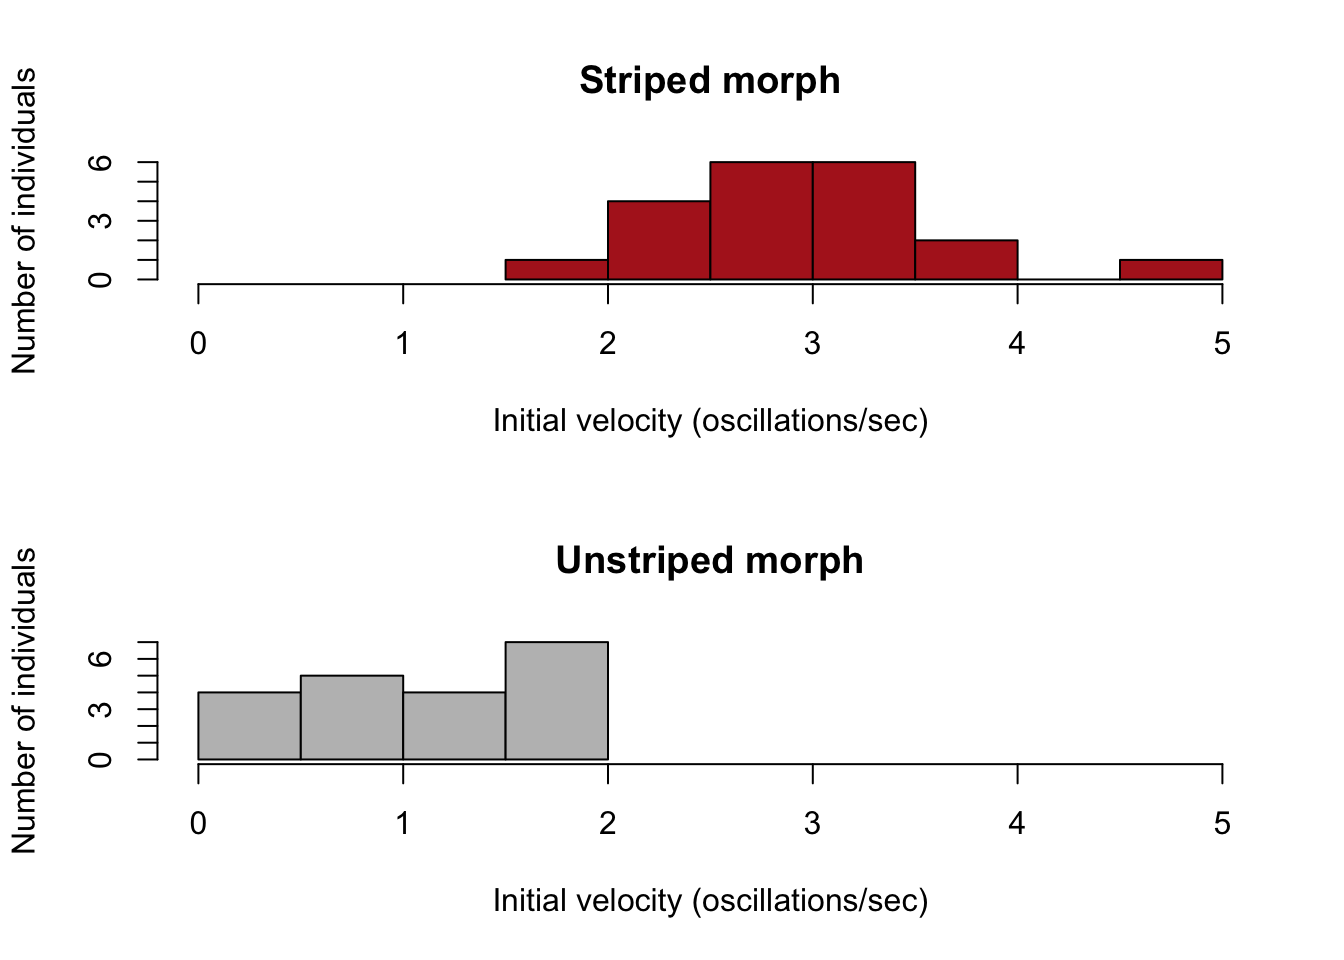
\includegraphics[width=0.7\linewidth]{Research-Design---Statistics_files/figure-latex/unnamed-chunk-3-1} \caption{Histograms of initial tail velocity for striped and unstriped color morphs.}\label{fig:unnamed-chunk-3}
\end{figure}

Note that I set the x-axis limits to be the same so that we have a fair comparison between the morphs. We clearly see that the distribution of initial velocity is much lower for the unstriped than the striped morph.

\subsubsection{Approaches without manually subsetting}\label{approaches-without-manually-subsetting}

In some cases we can plot the distribution of quantitative variables separately by groups without manually subsetting our data frame. This is often done by using our formula notation. For example, here we create \textbf{box plots} comparing the distributions of velocity between morphs:

\begin{Shaded}
\begin{Highlighting}[]
\FunctionTok{boxplot}\NormalTok{(tail}\SpecialCharTok{$}\NormalTok{tail.vel }\SpecialCharTok{\textasciitilde{}}\NormalTok{ tail}\SpecialCharTok{$}\NormalTok{morph, }\AttributeTok{col=}\FunctionTok{c}\NormalTok{(}\StringTok{"firebrick"}\NormalTok{, }\StringTok{"gray"}\NormalTok{),}
        \AttributeTok{xlab=}\StringTok{"Color morph"}\NormalTok{, }\AttributeTok{ylab=}\StringTok{"Oscillations/sec"}\NormalTok{)}
\end{Highlighting}
\end{Shaded}

\begin{center}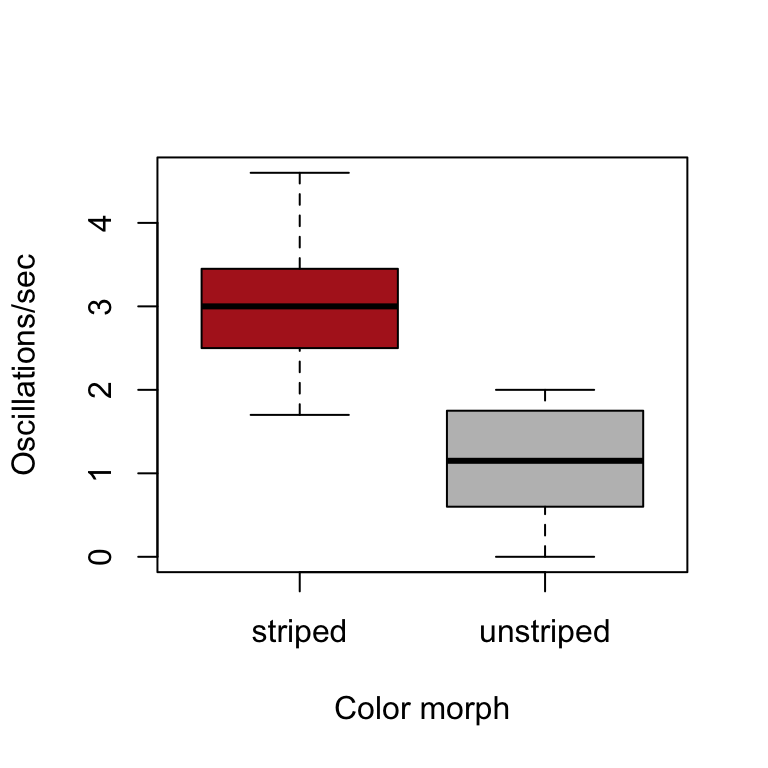
\includegraphics{Research-Design---Statistics_files/figure-latex/c3c85-1} \end{center}

Boxplots provide an alternative visual representation of the distribution of a quantitative varaible by displaying particular numerical summaries:

\begin{itemize}
\item
  Median: represented by the thick horizontal line as a metric of central tendency.
\item
  IQR: represented by the edges of the box, where the lower edge is the 25th percentile and the upper edge is the 75th percentile. The box displays the bounds of the middle 50\% of the data, giving you a sense for variation.
\item
  Variation in the tails: Values in the tails of the distribution are displayed by the whiskers, which extend up to 1.5 times the IQR from the box. Any values outside the whiskers are defined as \textbf{outliers} and are displayed by points.
\end{itemize}

The shape of a distribution can be inferred from a box plot based on the symmetry of the box and whiskers. If the box and whiskers are largely symmetrical, then the distribution has a bell shape. If the box and whisker extends far from the median to one end of the distribution, then the distribution is skewed.

So what does all this mean for comparing initial velocity between color morphs? We can see that the shape of the initial velocity distribution is similar between color morphs, being bell-shaped for both morphs. The variation among individuals also appears largely consistent between morphs. Clearly, however, the distribution of initial velocity differ dramatically in central tendency. The distribution of initial velocity is shifted to greater values for the striped morph than the unstriped morph.

One of the downsides of boxplots is that you don't see the individual data points. An alternative type of figure that's useful for showing all the data is a \textbf{stripchart}. The tradeoff is that strip charts don't show any summary statistics of central tendency or variation, but those statistics can be added separately. Here's a stripchart comparing initial velocity between color morphs.

\begin{Shaded}
\begin{Highlighting}[]
\FunctionTok{stripchart}\NormalTok{(tail}\SpecialCharTok{$}\NormalTok{tail.vel }\SpecialCharTok{\textasciitilde{}}\NormalTok{ tail}\SpecialCharTok{$}\NormalTok{morph, }\AttributeTok{col=}\FunctionTok{c}\NormalTok{(}\StringTok{"firebrick"}\NormalTok{, }\StringTok{"gray"}\NormalTok{),}
           \AttributeTok{xlab=}\StringTok{"Color morph"}\NormalTok{, }\AttributeTok{ylab=}\StringTok{"Oscillations/sec"}\NormalTok{, }\AttributeTok{cex.lab=}\FloatTok{1.2}\NormalTok{,}
           \AttributeTok{vertical=}\ConstantTok{TRUE}\NormalTok{, }\AttributeTok{method=}\StringTok{"jitter"}\NormalTok{, }\AttributeTok{jitter=}\FloatTok{0.15}\NormalTok{, }\AttributeTok{pch=}\DecValTok{1}\NormalTok{)}

\DocumentationTok{\#\# quantify means, sds, sample sizes, standard errors, and lower/upper confidence limits}
\NormalTok{morph.vel.means }\OtherTok{\textless{}{-}} \FunctionTok{aggregate}\NormalTok{(tail}\SpecialCharTok{$}\NormalTok{tail.vel, }\FunctionTok{list}\NormalTok{(tail}\SpecialCharTok{$}\NormalTok{morph), }\AttributeTok{FUN=}\NormalTok{mean)}
\NormalTok{morph.vel.sd }\OtherTok{\textless{}{-}} \FunctionTok{aggregate}\NormalTok{(tail}\SpecialCharTok{$}\NormalTok{tail.vel, }\FunctionTok{list}\NormalTok{(tail}\SpecialCharTok{$}\NormalTok{morph), }\AttributeTok{FUN=}\NormalTok{sd)}

\DocumentationTok{\#\# add standard deviation}
\FunctionTok{segments}\NormalTok{(}\FunctionTok{c}\NormalTok{(}\FloatTok{0.75}\NormalTok{, }\FloatTok{1.75}\NormalTok{), morph.vel.means}\SpecialCharTok{$}\NormalTok{x }\SpecialCharTok{{-}}\NormalTok{ morph.vel.sd}\SpecialCharTok{$}\NormalTok{x,}
         \FunctionTok{c}\NormalTok{(}\FloatTok{0.75}\NormalTok{, }\FloatTok{1.75}\NormalTok{), morph.vel.means}\SpecialCharTok{$}\NormalTok{x }\SpecialCharTok{+}\NormalTok{ morph.vel.sd}\SpecialCharTok{$}\NormalTok{x)}

\DocumentationTok{\#\# now add the means}
\FunctionTok{points}\NormalTok{(}\FunctionTok{c}\NormalTok{(}\FloatTok{0.75}\NormalTok{,}\FloatTok{1.75}\NormalTok{), morph.vel.means}\SpecialCharTok{$}\NormalTok{x,          }
       \AttributeTok{pch=}\DecValTok{19}\NormalTok{, }\AttributeTok{cex=}\DecValTok{2}\NormalTok{, }\AttributeTok{col=}\FunctionTok{c}\NormalTok{(}\StringTok{"firebrick"}\NormalTok{, }\StringTok{"gray"}\NormalTok{))}
\end{Highlighting}
\end{Shaded}

\begin{center}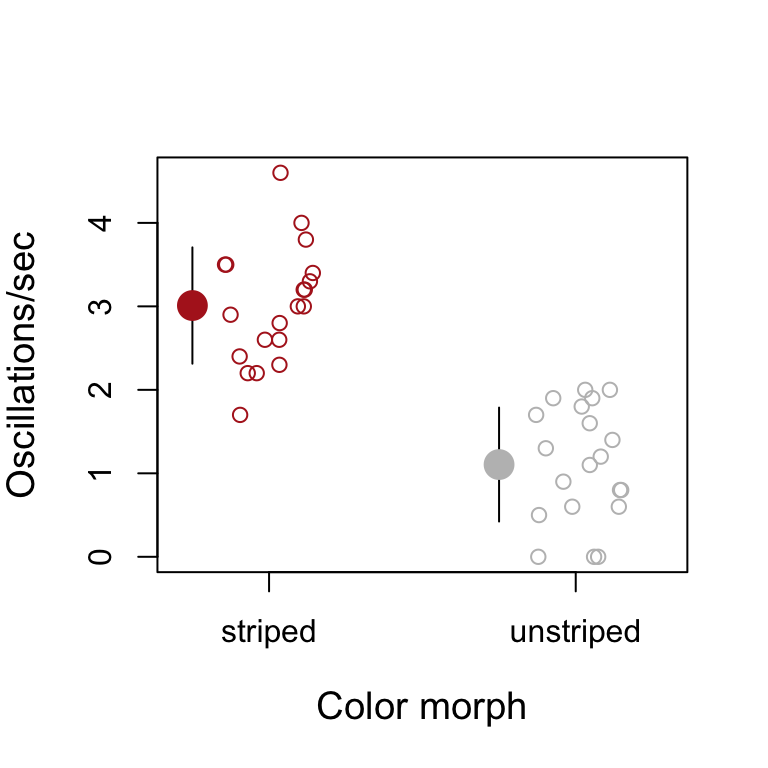
\includegraphics{Research-Design---Statistics_files/figure-latex/c3c86-1} \end{center}

Wow, things are getting complicated! Don't worry and don't feel overwhelmed. There is a learning curve to R, and I'm even including some quantitative metrics here that we won't cover in detail until later chapters. But let's break down what this strip chart is showing:

\begin{itemize}
\item
  Open circles: These represent the observed data points. These are added by the stripchart function. Note that I've color-coded each morph, which isn't completely necessary but can add a nice visual touch. Other new arguments here are \texttt{vertical}, which I've used to make the stripchart orient vertically, and \texttt{jitter}, which is used to add some random distance among the points along the x-axis. The jitter is useful to make points with very similar measurements more distinct.
\item
  Closed circles: These are the estimated means. Notice that I didn't simply use the mean function directly to quantify these. Because I wanted to estiamte the mean separately for each group, I had to use a new function: \texttt{aggregate}. The \texttt{aggregate} function allows you to compute a descriptive statistic separately by groups that you've defined, in this case the \textbf{morph}. Notice that I also computed the standard deviation by color morph with the aggregate function.
\end{itemize}

*Thin black lines: These are error bars representing one standard deviation away from the mean. Recall that the standard deviation is a descriptive metric of variation among individuals in a dataset.

So what does this graph tell us? Well, it tells us largely the same thing we saw with the box plots, except this time with all of the data visualized and with some different descriptive statistics. We can see that the standard deviation is very similar between color morphs, but the means appear to differ quite a bit.

Based on these graphs, can we conclude that the striped morphs have greater initial velocity in their autotomized tails than the unstriped morphs? You might be tempted to do so, but all we have done to this point is \emph{describe} the data. If you want to make a conclusion about whether something like the mean differs between groups, then you need different statistical tools, namely the tools of \textbf{inferential statistics}. Why? We'll discover the reasons in detail later in the book, but to hold you over, the main reason we can't make an inference about hte difference in means is because those means are \textbf{estimates}, and estimates have uncertainty. We need tools to examine that uncertainty before we can make any rigorous comparison of the mean between the groups of interest. More to come!

\subsection{Associations between qualitative variables}\label{associations-between-qualitative-variables}

Examining associations between categorical variables is even simpler in some ways. Let's consider another example from the squirrel dataset. Recall that squirrels were described by their primary fur color. Might behavior vary among individuals with different primary fur color? As just one example, for each squirrel in the dataset, the observer recorded whether or not the individual was climbing at the time it was observed. To examine the association, we can compute the proportion of squirrels observed climbining within each category of primary fur color:

\begin{Shaded}
\begin{Highlighting}[]
\DocumentationTok{\#\# quantify proportion climbing by fur color}
\NormalTok{p.climb }\OtherTok{\textless{}{-}} \FunctionTok{aggregate}\NormalTok{(climbing }\SpecialCharTok{\textasciitilde{}}\NormalTok{ primary.fur.color, }\AttributeTok{data =}\NormalTok{ sq, }\AttributeTok{FUN =}\NormalTok{ mean)}

\CommentTok{\# Plot}
\FunctionTok{barplot}\NormalTok{(}
  \AttributeTok{height =}\NormalTok{ p.climb}\SpecialCharTok{$}\NormalTok{climbing,}
  \AttributeTok{ylim=}\FunctionTok{c}\NormalTok{(}\DecValTok{0}\NormalTok{, }\FloatTok{0.25}\NormalTok{),}
  \AttributeTok{names.arg =}\NormalTok{ p.climb}\SpecialCharTok{$}\NormalTok{primary.fur.color,}
  \AttributeTok{xlab =} \StringTok{"Primary Fur Color"}\NormalTok{,}
  \AttributeTok{ylab =} \StringTok{"Proportion Climbing"}\NormalTok{,}
  \AttributeTok{col =} \FunctionTok{c}\NormalTok{(}\StringTok{"black"}\NormalTok{, }\StringTok{"brown"}\NormalTok{, }\StringTok{"gray"}\NormalTok{)}
\NormalTok{)}
\end{Highlighting}
\end{Shaded}

\begin{center}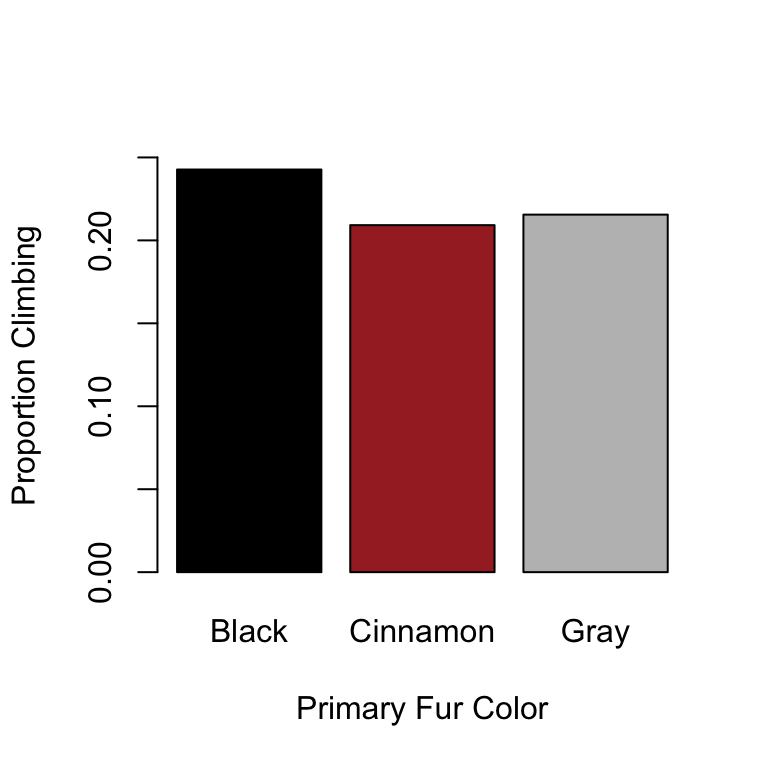
\includegraphics{Research-Design---Statistics_files/figure-latex/c3c87-1} \end{center}

Here I used the aggregate function again, this time to quantify the proportion climbing by categories of \texttt{primary.fur.color}. Notice that the function I used to quantify the proportion climbing within each category is the mean. Interesting! How does that work? Well, recall that climbing is defined as a logical variable, being TRUE for individuals who were observed climbing, and FALSE for those that weren't climbing. When a mathematical function is applied to a logic variable, R treats the variable as a binary numeric variable with values of 0 and 1. The TRUE observations are defined as 1, and the FALSE observations are defined as 0. Suppose we five observations of climbing were \{TRUE, FALSE, FALSE, TRUE, FALSE\}. If I quantify the mean of that variable, R converts the variable to \{1, 0, 0, 1, 0\}, and then quantifies the mean as

\[
\hat{\mu} = \frac{1 + 0 + 0 + 1 + 0}{5}=0.4
\]

The mean of a binary variable with values of 0 and 1s is the same as the proportion:

\[
\hat{p}_{\text{climbing}} = \frac{2}{5} = 0.4
\]

Cool!

Now, all we've done here is describe the observed data. Is the probability of climbing different among the categories of primary fur color? Our descriptive estimates of the proportion climbing are definitely different, but remember this is only a description of estimates that have uncertainty. We need to examine that uncertainty to inform our conclusion about whether climbing behavior really differs among these groups. Stay tuned!

\section{Some final points about R}\label{some-final-points-about-r}

\subsection{Packages}\label{packages}

All of the R code that we executed in R was done with the basic functionality that comes with R when first installed. But one of the best things about R is that anyone can write their own functions and share them with others via packages. For example, all of the plots that I created above were created with base R functions, but there are many other packages that others have developed that can be used to create plots. One of the most popular of those packages is called \texttt{ggplot2}, so let's take a look at it.

\subsection{Installing a package}\label{installing-a-package}

When you want to use functions from a specialized package in R, you first have to install the package with those functions. You can install packages with the \texttt{install.packages} function. The main argument of the \texttt{install.packages} function is a character vector of the packages you want to install. If you only want to install a single package, just write the name of the package as a character:

\begin{Shaded}
\begin{Highlighting}[]
\FunctionTok{install.packages}\NormalTok{(}\StringTok{"ggplot2"}\NormalTok{)}
\end{Highlighting}
\end{Shaded}

\begin{verbatim}
## Error in install.packages : Updating loaded packages
\end{verbatim}

When you execute the code, you'll see R will download the package and install it.

\subsection{Using functions from a package}\label{using-functions-from-a-package}

After you've installed a package, you can start to use functions from the package, but to do so, you have to tell R you want to use the functions in that package. One way to do this is to load the package with the \texttt{library} function:

\begin{Shaded}
\begin{Highlighting}[]
\FunctionTok{library}\NormalTok{(ggplot2)}
\end{Highlighting}
\end{Shaded}

Once you execute the code to load the package, you can then use any function in the package just as you'd use functions from base R. For example, we can use the ggplot function to create the scatterplot we created above relating the length and mass of salamanders:

\begin{Shaded}
\begin{Highlighting}[]
\FunctionTok{ggplot}\NormalTok{(tail, }\FunctionTok{aes}\NormalTok{(}\AttributeTok{x =}\NormalTok{ length.cm, }\AttributeTok{y =}\NormalTok{ mass.g)) }\SpecialCharTok{+}
  \FunctionTok{geom\_point}\NormalTok{(}\AttributeTok{shape =} \DecValTok{19}\NormalTok{) }\SpecialCharTok{+}
  \FunctionTok{labs}\NormalTok{(}\AttributeTok{x =} \StringTok{"Snout{-}vent length (cm)"}\NormalTok{, }\AttributeTok{y =} \StringTok{"Mass (g)"}\NormalTok{, }\AttributeTok{title =} \StringTok{""}\NormalTok{)}
\end{Highlighting}
\end{Shaded}

\begin{center}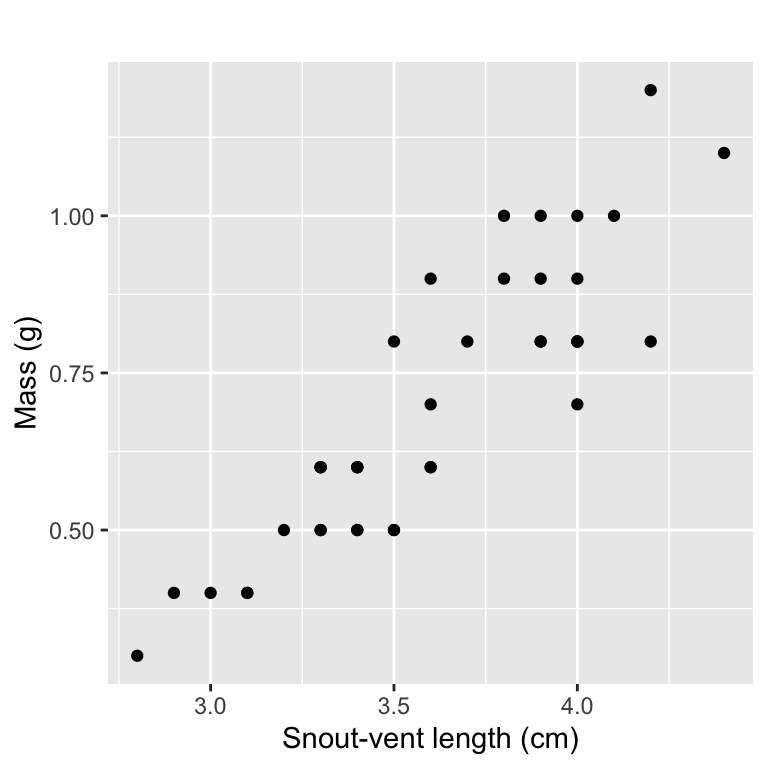
\includegraphics{Research-Design---Statistics_files/figure-latex/c3c90-1} \end{center}

The ggplot function has it's own quirks, one of which is that it works with a hierarchical set of functions. Most directly we specified that a plot will be created with the tail data frame, but then we used the \texttt{aes} function from ggplot to describe which variables in the tail data frame should be associated, in this case placing mass on the y-axis and length on the x-axis. But additional components need to be specified with susbequent functions, called ``layers''. Different layers are added to the graph using the layer operator, \texttt{+}. To improve readability, the \texttt{+} operator is often placed at the end of each line when breaking up commands across multiple lines.

Let me show you what I mean. Suppose I only executed the first line of code without the layer operator and subsequeent layers. Let's do that and see what the plot looks like:

\begin{Shaded}
\begin{Highlighting}[]
\FunctionTok{ggplot}\NormalTok{(tail, }\FunctionTok{aes}\NormalTok{(}\AttributeTok{x =}\NormalTok{ length.cm, }\AttributeTok{y =}\NormalTok{ mass.g))}
\end{Highlighting}
\end{Shaded}

\begin{center}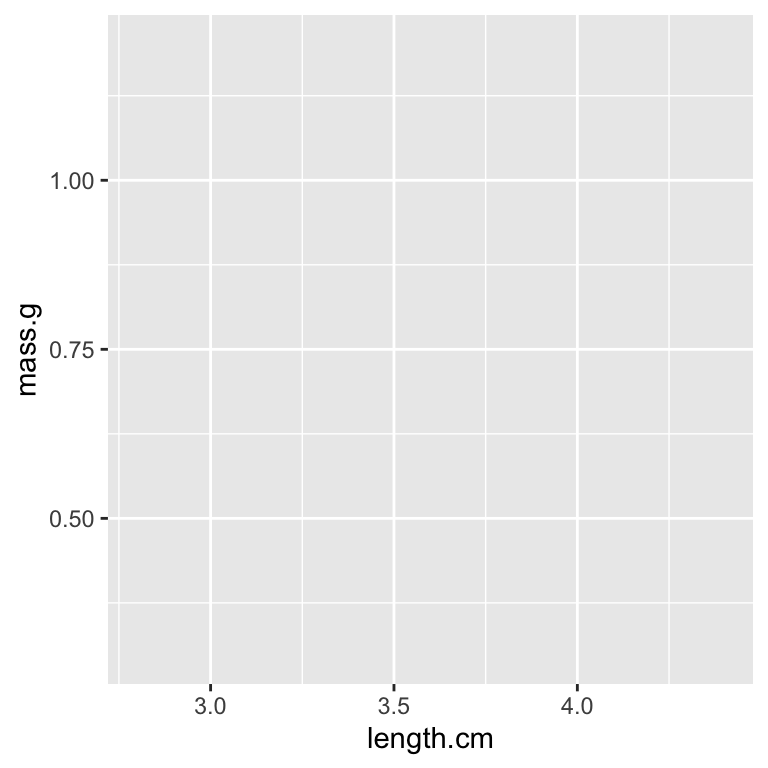
\includegraphics{Research-Design---Statistics_files/figure-latex/c3c91-1} \end{center}

It's incompelte. It put the names of the vector I wanted on the x- and y-axes, but it didn't plot any points. The points get plotted with the \texttt{geom\_point} layer, specifying the points with shape = 19, which is simply a closed circle:

\begin{Shaded}
\begin{Highlighting}[]
\FunctionTok{ggplot}\NormalTok{(tail, }\FunctionTok{aes}\NormalTok{(}\AttributeTok{x =}\NormalTok{ length.cm, }\AttributeTok{y =}\NormalTok{ mass.g)) }\SpecialCharTok{+}
  \FunctionTok{geom\_point}\NormalTok{(}\AttributeTok{shape =} \DecValTok{19}\NormalTok{) }
\end{Highlighting}
\end{Shaded}

\begin{center}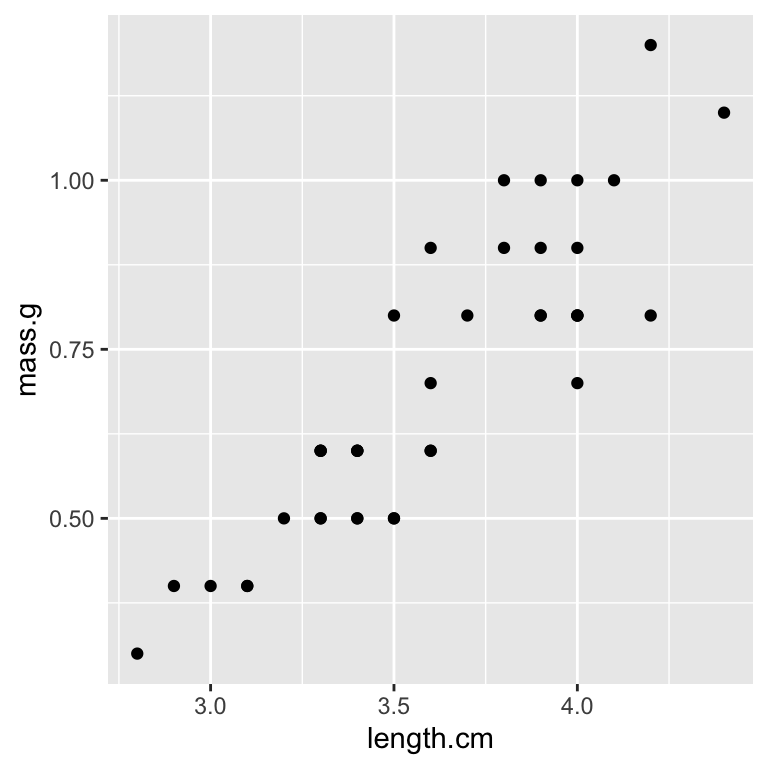
\includegraphics{Research-Design---Statistics_files/figure-latex/c3c92-1} \end{center}

Now we see the points, but to label the x- and y-axes correctly, you have to add another layer via the \texttt{labs} function.

\begin{Shaded}
\begin{Highlighting}[]
\FunctionTok{ggplot}\NormalTok{(tail, }\FunctionTok{aes}\NormalTok{(}\AttributeTok{x =}\NormalTok{ length.cm, }\AttributeTok{y =}\NormalTok{ mass.g)) }\SpecialCharTok{+}
  \FunctionTok{geom\_point}\NormalTok{(}\AttributeTok{shape =} \DecValTok{19}\NormalTok{) }\SpecialCharTok{+}
  \FunctionTok{labs}\NormalTok{(}\AttributeTok{x =} \StringTok{"Snout{-}vent length (cm)"}\NormalTok{, }\AttributeTok{y =} \StringTok{"Mass (g)"}\NormalTok{, }\AttributeTok{title =} \StringTok{""}\NormalTok{)}
\end{Highlighting}
\end{Shaded}

\begin{center}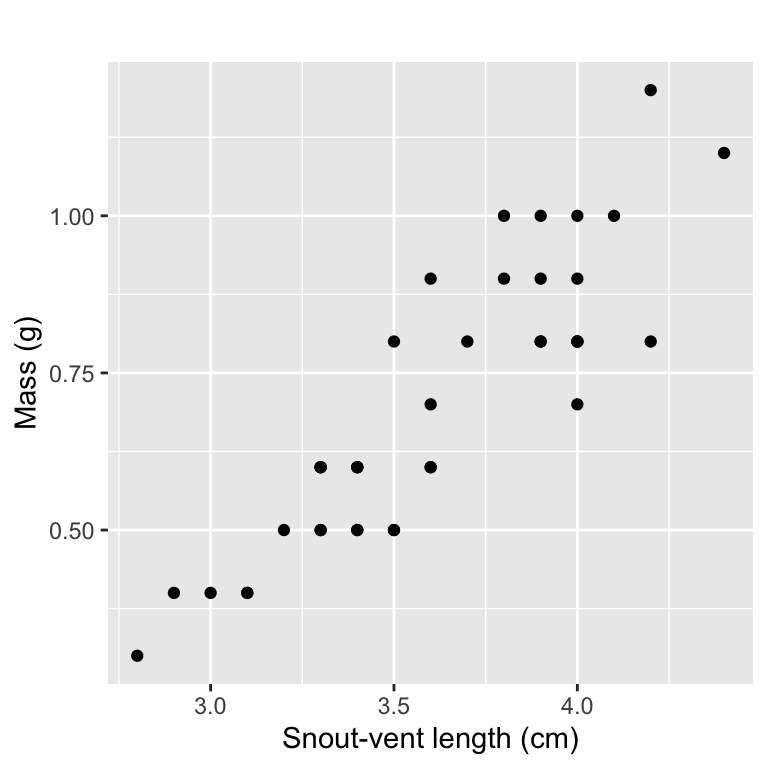
\includegraphics{Research-Design---Statistics_files/figure-latex/c3c93-1} \end{center}

All of the types of graphs I created above could be created with ggplot2. For example:

\begin{Shaded}
\begin{Highlighting}[]
\FunctionTok{ggplot}\NormalTok{(tail, }\FunctionTok{aes}\NormalTok{(}\AttributeTok{x =}\NormalTok{ tail.vel)) }\SpecialCharTok{+}
  \FunctionTok{geom\_histogram}\NormalTok{(}\AttributeTok{binwidth =} \FloatTok{0.5}\NormalTok{, }\AttributeTok{color =} \StringTok{"black"}\NormalTok{, }\AttributeTok{fill =} \StringTok{"lightblue"}\NormalTok{) }\SpecialCharTok{+} 
  \FunctionTok{labs}\NormalTok{(}\AttributeTok{x =} \StringTok{"Initial velocity (oscillations/sec)"}\NormalTok{, }\AttributeTok{y =} \StringTok{"Number of individuals"}\NormalTok{)}
\end{Highlighting}
\end{Shaded}

\begin{center}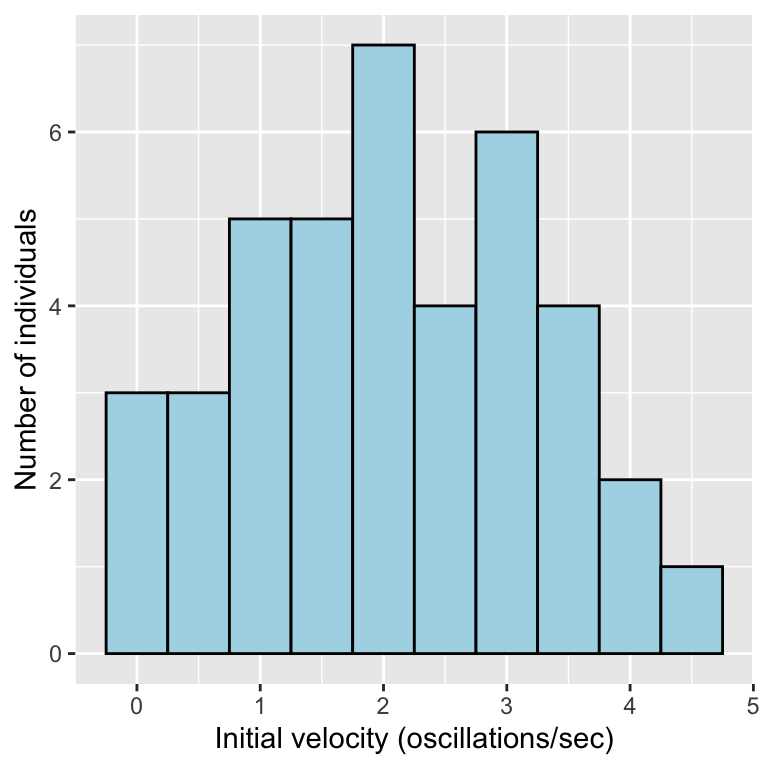
\includegraphics{Research-Design---Statistics_files/figure-latex/c3c94-1} \end{center}

\begin{Shaded}
\begin{Highlighting}[]
\FunctionTok{ggplot}\NormalTok{(tail, }\FunctionTok{aes}\NormalTok{(}\AttributeTok{x =} \StringTok{""}\NormalTok{, }\AttributeTok{y =}\NormalTok{ tail.vel)) }\SpecialCharTok{+}
  \FunctionTok{geom\_boxplot}\NormalTok{() }\SpecialCharTok{+}
  \FunctionTok{labs}\NormalTok{(}\AttributeTok{x =} \StringTok{"Initial velocity"}\NormalTok{, }\AttributeTok{y =} \StringTok{"Oscillations/sec"}\NormalTok{)}
\end{Highlighting}
\end{Shaded}

\begin{center}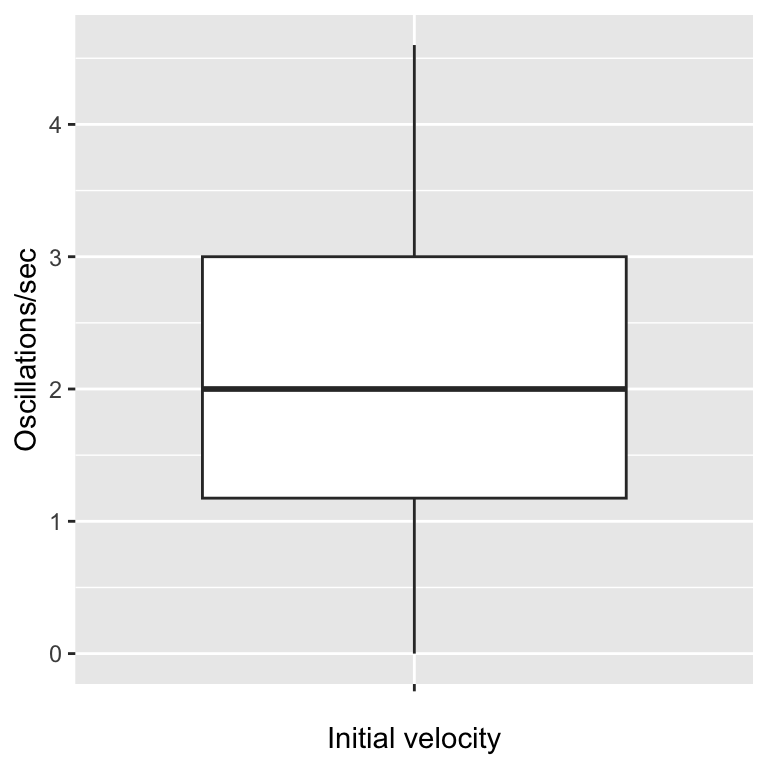
\includegraphics{Research-Design---Statistics_files/figure-latex/c3c94-2} \end{center}

\begin{Shaded}
\begin{Highlighting}[]
\FunctionTok{ggplot}\NormalTok{(tail, }\FunctionTok{aes}\NormalTok{(}\AttributeTok{x =} \StringTok{""}\NormalTok{, }\AttributeTok{y =}\NormalTok{ tail.vel)) }\SpecialCharTok{+}
  \FunctionTok{geom\_jitter}\NormalTok{(}\AttributeTok{width =} \FloatTok{0.2}\NormalTok{, }\AttributeTok{shape =} \DecValTok{1}\NormalTok{) }\SpecialCharTok{+} 
  \FunctionTok{labs}\NormalTok{(}\AttributeTok{x =} \StringTok{"Initial velocity"}\NormalTok{, }\AttributeTok{y =} \StringTok{"Oscillations/sec"}\NormalTok{)}
\end{Highlighting}
\end{Shaded}

\begin{center}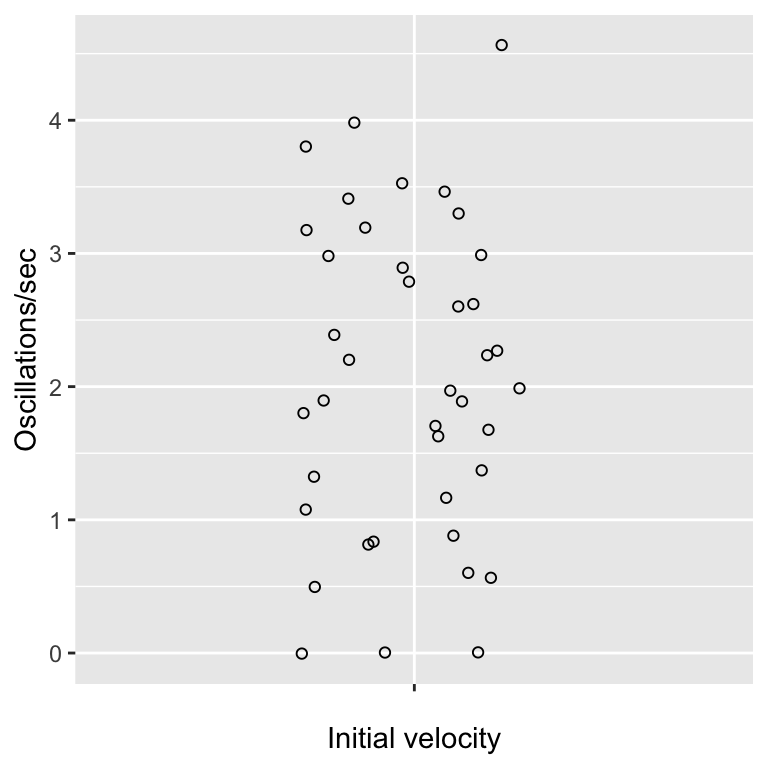
\includegraphics{Research-Design---Statistics_files/figure-latex/c3c94-3} \end{center}

The \texttt{ggplot2} package is especially useful for making multipanel plots. For example, suppose we wanted to create the figure of histograms of initial velocity for each salamander morph.

\begin{Shaded}
\begin{Highlighting}[]
\FunctionTok{ggplot}\NormalTok{(tail, }\FunctionTok{aes}\NormalTok{(}\AttributeTok{x =}\NormalTok{ tail.vel, }\AttributeTok{fill =}\NormalTok{ morph)) }\SpecialCharTok{+}
  \FunctionTok{geom\_histogram}\NormalTok{(}\AttributeTok{binwidth =} \FloatTok{0.5}\NormalTok{, }\AttributeTok{color =} \StringTok{"black"}\NormalTok{) }\SpecialCharTok{+}  \CommentTok{\# Adjust bin width as needed}
  \FunctionTok{scale\_fill\_manual}\NormalTok{(}\AttributeTok{values =} \FunctionTok{c}\NormalTok{(}\StringTok{"striped"} \OtherTok{=} \StringTok{"firebrick"}\NormalTok{, }\StringTok{"unstriped"} \OtherTok{=} \StringTok{"gray"}\NormalTok{)) }\SpecialCharTok{+}
  \FunctionTok{facet\_wrap}\NormalTok{(}\SpecialCharTok{\textasciitilde{}}\NormalTok{ morph, }\AttributeTok{ncol =} \DecValTok{1}\NormalTok{) }\SpecialCharTok{+}  \CommentTok{\#plot by morph in one column}
  \FunctionTok{xlim}\NormalTok{(}\DecValTok{0}\NormalTok{, }\DecValTok{5}\NormalTok{) }\SpecialCharTok{+}
  \FunctionTok{labs}\NormalTok{(}\AttributeTok{x =} \StringTok{"Initial velocity (oscillations/sec)"}\NormalTok{, }\AttributeTok{y =} \StringTok{"Number of individuals"}\NormalTok{) }\SpecialCharTok{+}
  \FunctionTok{theme}\NormalTok{(}\AttributeTok{legend.position =} \StringTok{"none"}\NormalTok{)  }\CommentTok{\#suppress legend, not needed}
\end{Highlighting}
\end{Shaded}

\begin{verbatim}
## Warning: Removed 4 rows containing missing values or values outside the scale range
## (`geom_bar()`).
\end{verbatim}

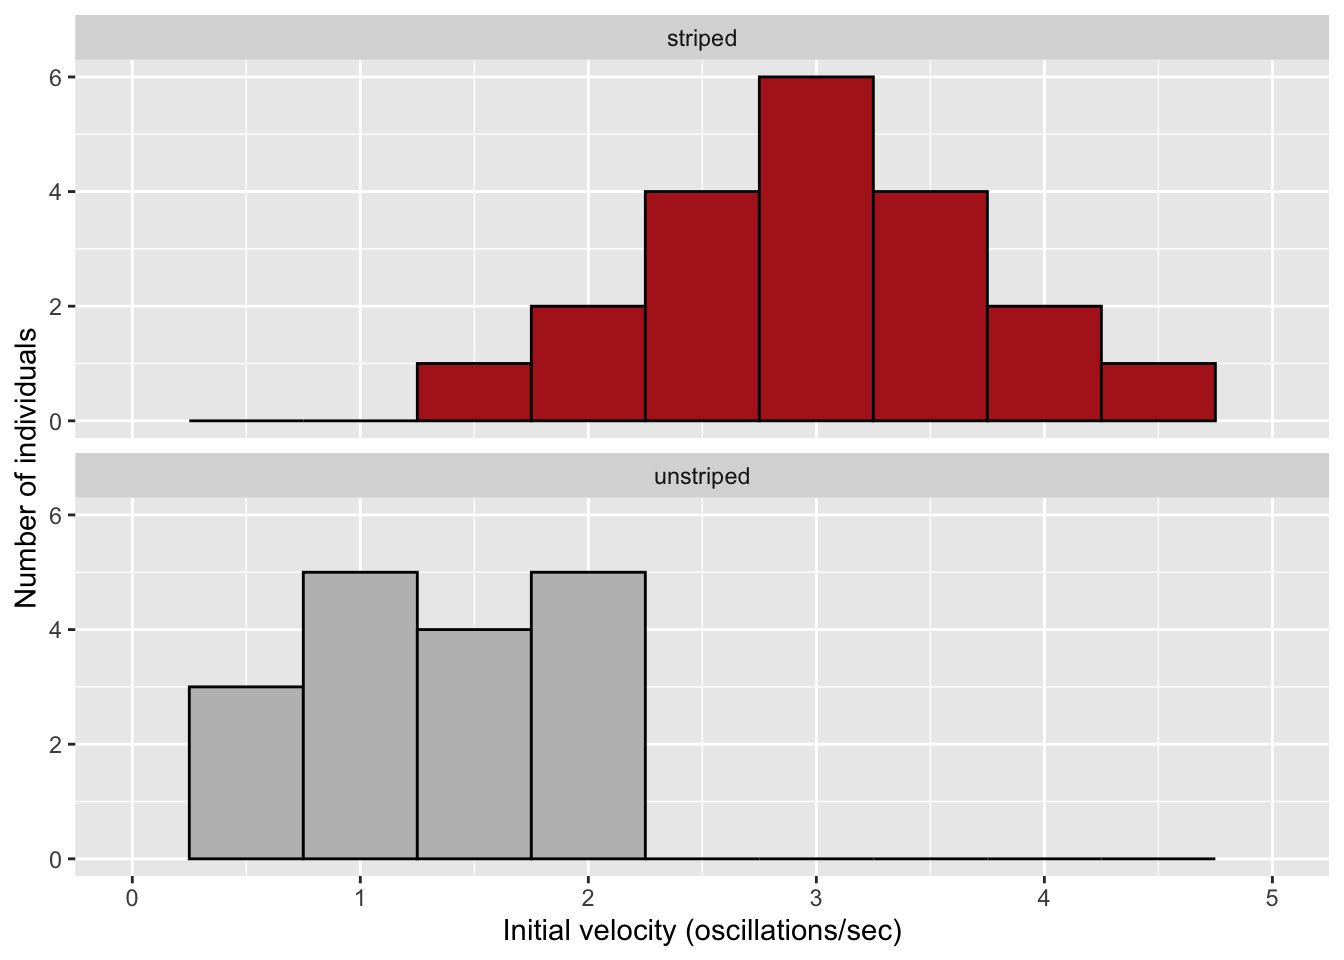
\includegraphics{Research-Design---Statistics_files/figure-latex/unnamed-chunk-4-1.pdf}

Compared to the single histogram above, we've added a few arguments to make this a multipanel plot. First, we specify \texttt{fill\ =\ morph} in the \texttt{aes} function to indicate that we want the histogram colors to vary between morph. The \texttt{scale\_fill\_manual} layer allows us to specify the colors we want for each morph. Second, we use the \texttt{facet\_wrap} argument to create the multipanel plot, specifying \texttt{\textasciitilde{}\ morph} so R knows to subset the data by morph, and then \texttt{ncol\ =\ 1} so R knows to plot the histograms in a single column. Multipanel plots in \texttt{ggplot2} will usually have labels on each panel, so usually don't need an additional legend, which we've suppressed with \texttt{theme(legend.position\ =\ "none")}.

\subsection{Scripting}\label{scripting}

One last R skill that I'd like to briefly cover is scripting. Doing analysis by coding is great for a variety of reasons, but one of the best reasons to code is to make your science reproducible with a script. When you execute a set o functions for an analysis, you can save the code to execute those functions in a script, which is basically a text file (with an .R extension).

Suppose you're working on an analysis for an hour and then the power goes out. Well, if you were scripting your analysis, all you have to do is load your script and execute all the functions up to the point where you left off. A script allows you go back and easily make changes, and it allows others to see \emph{exactly} how you performed an analysis. Indeed, most scientific journals are now requiring that authors publish their code used to conduct analyses to be completely transparent about how the analyses were performed.

How do you make a script? It's really easy in RStudio? In your toolbar, just click File, New File, and then R script. That will open a text editor in the top left panel of RStudio. From there you can start writing your code. I strongly recommend that you add notes to your code to describe what the code is doing. These notes don't have to be extensive, but it's very useful to help reorient yourself, or orient someone else for the first time, to what the code is doing.

For example, Figure \ref{fig:c3f4} shows a simple script that I wrote to perform some basic descriptive statistics on the salamander tails data. I included some notes to delineate different sections of the script. The dashes are not necessary, but I often use them because they allow me to visually demarcate the different sections of the script, and RStudio recognizes those sections and allows you to navigate among the different sections using the drop-down in the bottom left corner of the script panel.

\begin{figure}
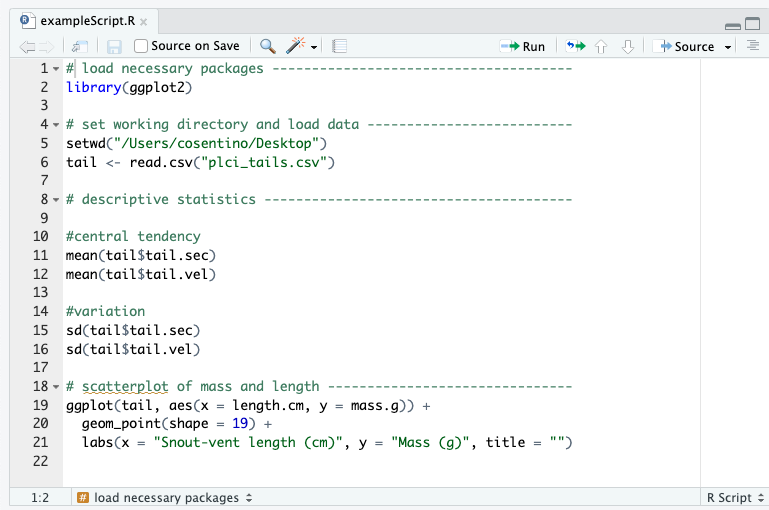
\includegraphics[width=0.9\linewidth]{images/03_exampleScript} \caption{Unstriped (left) and striped color morphs of red-backed salamanders.}\label{fig:c3f4}
\end{figure}

How do you execute the code in a script? It's easy! Just highlight the code that you want to execute, then click the ``Run'' button in the top right corner of the script panel. You'll see the code executed in the R console in the bottom left panel, along with any generated output.

\chapter{Graphical Causal Models}\label{graphical-causal-models}

I've made the case that science starts with a clear research question, and we've explored some characteristics of what defines a good research question. I've also suggested that many (maybe most) scientific research studies have a primary goal of testing a causal hypothesis. In this chapter, we will take a closer look at causal questions. Designing scientific studies to address causal questions can be extremely challenging. Overcoming those challenges requires a clearly stated scientific model of the causal effects being hypothesized. Describing your scientific model and stating your causal assumptions with a graph is the focus of this chapter, and a theme that we will come back to as we explore the particulars of research design and statistics in the remainder of the book.

\section{Directed acyclic graphs (DAGs)}\label{directed-acyclic-graphs-dags}

There are two general approaches to \textbf{causal inference}: the potential outcomes framework (\href{https://www.jstor.org/stable/2245382}{Neyman 1923}, \href{https://www.jstor.org/stable/27590541}{Rubin 2005}) and the graphical causal model framework (\href{https://bayes.cs.ucla.edu/BOOK-2K/}{Pearl 2000}). In this book, we will use graphical causal models to guide our approach to causal inference. I find that the graphical representation of causal models provides for a smoother entry to the ideas of causal inference for students in an introductory statistics course.

The graphical causal modeling framework uses \textbf{directed acyclic graphs (DAGs)} to visualize the causal assumptions of a hypothesis. Let's work through an example. Suppose you are interested in the causal effect of living near urban greenspace on mental health. In cities, greenspaces are simply areas where natural vegetation occurs, such as forest. This is a forward causal question with a clearly defined cause (greenspace) and effect (mental health). The hypothesis is that living near greenspace reduces the risk of mental health disorders, perhaps by alleviating anxiety, or encouraging physical activity. Causal effects of one variable on another can involve multiple mechanisms.

Let's assume that we can measure whether or not people live near greenspace. We define \texttt{greenspace} as a nominal variable where individuals live either ``near greenspace'' or ``not near greenspace''. In reality, proximity to greenspace can be measured on a continuum, but for now let's keep it simple and define proximity categorically. Let's also assume that \texttt{mental.health} is a binary, categorical variable. People either have a mental health disorder, or they don't.

Our causal hypothesis is represented as a DAG in Figure \ref{fig:c4c1}. This kind of graph has nodes that represent variables, and arrows between nodes that illustrate the flow of causation. Based on how we've talked about our research question to this point, we have a really simple DAG. The nodes are greenspace and mental health, and there's a directional arrow from greenspace to mental health. The direction of the arrow shows the direction of causality. This DAG implies that greenspace directly influences mental health. Because there are no other variables between these variables, we define the effect of greenspace on mental health as a \textbf{direct effect}.

\begin{Shaded}
\begin{Highlighting}[]
\FunctionTok{library}\NormalTok{(dagitty)}
\FunctionTok{library}\NormalTok{(rethinking)}
\NormalTok{dag1 }\OtherTok{\textless{}{-}} \FunctionTok{dagitty}\NormalTok{(}\StringTok{"dag \{greenspace {-}\textgreater{} mental.health\}"}\NormalTok{)}
\FunctionTok{coordinates}\NormalTok{(dag1) }\OtherTok{\textless{}{-}} \FunctionTok{list}\NormalTok{(}\AttributeTok{x =} \FunctionTok{c}\NormalTok{(}\AttributeTok{greenspace =} \DecValTok{0}\NormalTok{, }\AttributeTok{mental.health =} \DecValTok{1}\NormalTok{), }\AttributeTok{y =} \FunctionTok{c}\NormalTok{(}\AttributeTok{greenspace =} \DecValTok{0}\NormalTok{, }\AttributeTok{mental.health =} \DecValTok{0}\NormalTok{))}
\FunctionTok{drawdag}\NormalTok{(dag1)}
\end{Highlighting}
\end{Shaded}

\begin{figure}

{\centering 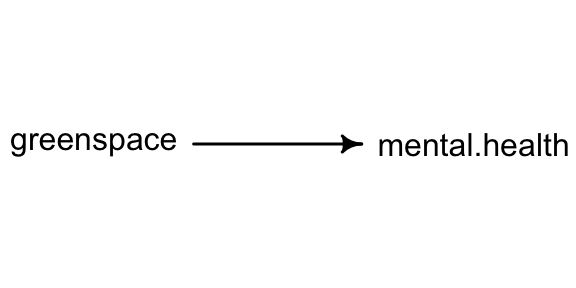
\includegraphics{Research-Design---Statistics_files/figure-latex/c4c1-1} 

}

\caption{Initial DAG for the causal effect of greenspace on mental health.}\label{fig:c4c1}
\end{figure}

Our hypothesis is that greenspace \emph{reduces} the risk of mental health disorders, but note there's no indication of the nature of the causal effect in the DAG. DAGs simply illustrate assumed causal effects. DAGs do not assume anything about the form of the causal relationship between variables (e.g., positive vs.~negative relationship, linear vs.~non-linear relationship).

Drawing DAGs

In this chapter and throughout the book I will create figures of DAGs in R with the \texttt{dagitty} and \texttt{rethinking} packages. The relationship between variables are defined by the \texttt{dagitty} function, with the arrow \texttt{-\textgreater{}} identifying the direction of causality between variables. You can use the \texttt{coordinates} function to customize the arrnangement of the variables in the plot along x- and y-axes.

I also highly recommend the \href{https://www.dagitty.net/}{dagitty website}, where you can draw DAGs directly in your internet browser.

Life is rarely so simple as assumed in our initial DAG. Notably, the DAG assumes that greenspace is the only significant cause of mental health. The emphasis on significant is purposeful. In reality, there may be hundreds of causes of mental health. Most outcomes in biology are like this with multiple possible causes. However, DAGs focus on the most important causes. If there's a particular mutation on a gene that increases the risk of a mental health disorder by 0.001\%, we probably don't need to include that in the DAG because the effect is trivial. Additionally, because we are focusing on mental health as an outcome, we don't necessarily need to include variables that are causally affected by mental health. Overall, some discretion about the variables to include in DAGs is warranted, because otherwise DAGs would be too complex to be useful (\href{https://theeffectbook.net/}{Huntington-Klein 2022}). All models are simplifications.

Suppose that we collect some idea, and we find that 18\% of individuals who don't live near greenspace have been diagnosed with a mental health disorder, whereas 11\% of individuals who live near greenspace have a mental health disorder. The absolute risk \footnote{\textbf{Absolute risk} is the probability that an event occurs, here expressed as a percentage. Absolute risk can be contrasted with \textbf{relative risk}, which is the proportional risk of one outcome relative to another. For example, if the absolute risk of a mental health disorder is 18\% for the ``near greenspace'' group and 11\% for the ``not near greenspace'' group, then the relative risk of living near greenspace is 0.11/0.18 = 0.61. This means that it is 0.61 times less likely to be diagnosed with a mental health disorder when living near greenspace relative to not living near greenspace. Relative risk and absolute risk are often reported in the medical literature, but note that relative risk doesn't tell you anything about the absolute risk. One useful way of comparing risk between groups on the absolute risk scale is the \textbf{absolute risk reduction}, which just the difference in absolute risk between groups. That's the 7\% that I referenced in the text.} of a mental health disorder is 7\% lower for individuals who live near greenspace. Is that difference caused by greenspace? Not necessarily! Why not? We need to consider the possibility that there is a common cause of greenspace and mental health. In other words, the people who live near greenspace differ in other ways from the people who don't live near greenspace, and these differences might contribute to mental health outcomes. One such possibility is socioeconomic status (SES). SES is very likely a cause of living near greenspace because wealthy people can afford to live near greenspace. SES might also be a cause of mental health because wealthy people have good access to healthcare. Figure \ref{fig:c4c2} adds SES to the DAG.

\begin{Shaded}
\begin{Highlighting}[]
\NormalTok{dag2 }\OtherTok{\textless{}{-}} \FunctionTok{dagitty}\NormalTok{(}\StringTok{"dag \{greenspace {-}\textgreater{} mental.health;}
\StringTok{                      SES {-}\textgreater{} greenspace;}
\StringTok{                      SES {-}\textgreater{} mental.health\}"}\NormalTok{)}
\FunctionTok{coordinates}\NormalTok{(dag2) }\OtherTok{\textless{}{-}} \FunctionTok{list}\NormalTok{(}\AttributeTok{x =} \FunctionTok{c}\NormalTok{(}\AttributeTok{greenspace =} \DecValTok{0}\NormalTok{, }\AttributeTok{SES =} \DecValTok{1}\NormalTok{, }\AttributeTok{mental.health =} \DecValTok{2}\NormalTok{), }
                          \AttributeTok{y =} \FunctionTok{c}\NormalTok{(}\AttributeTok{greenspace =} \DecValTok{0}\NormalTok{, }\AttributeTok{SES =} \SpecialCharTok{{-}}\DecValTok{1}\NormalTok{, }\AttributeTok{mental.health =} \DecValTok{0}\NormalTok{))}
\FunctionTok{drawdag}\NormalTok{(dag2)}
\end{Highlighting}
\end{Shaded}

\begin{figure}

{\centering 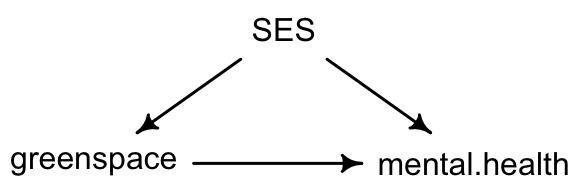
\includegraphics{Research-Design---Statistics_files/figure-latex/c4c2-1} 

}

\caption{DAG with the confounding variable SES added.}\label{fig:c4c2}
\end{figure}

The new DAG in Figure \ref{fig:c4c2} clearly identifies SES as a common cause of both greenspace and mental health. This means the causal relationship between greenspace and mental health is confounded by SES. We call SES a \textbf{confounding variable} because it affects both the explanatory and response variables, ultimately confusing our interpretation of the relationship between greenspace and mental health. Remember that the risk of having a mental health disorder was 7\% lower for people who live close to greenspace. It's possible that difference is due to a causal effect of greenspace on mental health, but it's also possible that some or all of the risk difference is due to the confounding effect of SES. Confounding variables can create associations between variables that are not causal.

Let me show you what I mean with the help of a data simulation. The risk probabilities of having a mental health disorder that I previously mentioned were generated by simulating data in R. Here's the code, followed by an explanation:

\begin{Shaded}
\begin{Highlighting}[]
\FunctionTok{set.seed}\NormalTok{(}\DecValTok{122}\NormalTok{)}

\DocumentationTok{\#\# simulate socioeconomic status (ses)}
\NormalTok{ses }\OtherTok{\textless{}{-}} \FunctionTok{rbinom}\NormalTok{(}\AttributeTok{n =} \DecValTok{1000}\NormalTok{, }\AttributeTok{size =} \DecValTok{1}\NormalTok{, }\AttributeTok{prob =} \FloatTok{0.5}\NormalTok{)}

\DocumentationTok{\#\# simulate green space access (grn) based on ses}
\NormalTok{grn }\OtherTok{\textless{}{-}} \FunctionTok{rbinom}\NormalTok{(}\AttributeTok{n =} \DecValTok{1000}\NormalTok{, }\AttributeTok{size =} \DecValTok{1}\NormalTok{, }\AttributeTok{prob =} \FunctionTok{ifelse}\NormalTok{(ses }\SpecialCharTok{==} \DecValTok{1}\NormalTok{, }\FloatTok{0.8}\NormalTok{, }\FloatTok{0.2}\NormalTok{))}

\DocumentationTok{\#\# simulate mental health status (mnt) based on ses}
\NormalTok{mnt }\OtherTok{\textless{}{-}} \FunctionTok{rbinom}\NormalTok{(}\AttributeTok{n =} \DecValTok{1000}\NormalTok{, }\AttributeTok{size =} \DecValTok{1}\NormalTok{, }\AttributeTok{prob =} \FunctionTok{ifelse}\NormalTok{(ses }\SpecialCharTok{==} \DecValTok{1}\NormalTok{, }\FloatTok{0.1}\NormalTok{, }\FloatTok{0.2}\NormalTok{))}
\end{Highlighting}
\end{Shaded}

I assumed that we have a dataset of \(n = 1000\) people, and for each person, I first randomly determined if they are of high or low socioeconomic status. I did this using a function called \texttt{rbinom}. The arguments of the \texttt{rbinom} function include the number of observations (\texttt{n\ =\ 1000}), the number of trials (\texttt{size\ =\ 1}), and the probability of ``success'' (\texttt{prob\ =\ 0.5}). What this means is that for each of the 1000 individuals, I determine a single time whether they are of high or low SES, each with a probability of 0.5. This produces the variable \texttt{ses}, a vector of 0 and 1 values, where 0 represents ``low ses'' and 1 represents ``high ses''. Because I set the probability of success to 0.5, there should be about a 50/50 split of low and high ses individuals. It won't necessarily be exactly 50\%, because the function is drawing values randomly. It's basically like flipping a coin 1000 times and counting heads and tails.

Once the ses variable was generated, I then generated the greenspace access variable, called \texttt{grn}. This was also generated with the \texttt{rbinom} function, where a 1 represents ``near greenspace'' and 0 represents ``not near greenspace''. I used the \texttt{ifelse} function to specify that the probability of being near greenspace was 0.8 for individuals of high ses and 0.2 for individuals of low ses. Finally, I generated a variable for mental health outcome, \texttt{mnt}, where 1 represents individuals who have a mental health disorder, and 0 represents individuals who don't have a mental health disorder. I assumed the probability of a mental health disorder was 0.1 for individuals of high ses and 0.2 for individuals of low ses. The only other part of the code chunk above is the \texttt{setseed} function, which allows you to simulate the exact same dataset that I simulated, as long as you use the same \texttt{setseed} number (122).

Now I want you to notice something important. Because we are simulating data, I had to make some assumptions about what the probability of a mental health disorder would be for individuals of high and low ses and individuals who are near or not near greenspace. In this simulation, I assumed that mental health risk is \emph{only} affected by SES. There is no direct effect of greenspace access on mental health risk based in this simulation. Let's see what happens when we compare the probability of a mental health disorder between greenspace access based on this simulated dataset. We can do that with the \texttt{table} function:

\begin{Shaded}
\begin{Highlighting}[]
\FunctionTok{table}\NormalTok{(mnt, grn)}
\end{Highlighting}
\end{Shaded}

\begin{verbatim}
##    grn
## mnt   0   1
##   0 421 436
##   1  90  53
\end{verbatim}

Here we see a \textbf{contingency table} showing the number of individuals in each category of mental health status and greenspace. Greenspace, the explanatory variable, is located at the top of the table, where the column for \texttt{grn} = 0 represents not near greenspace, and the column for \texttt{grn} = 1 represents individuals who live near greenspace. The rows represent the categories of mental health status, where \texttt{mnt} = 0 are the individuals who don't have a mental health disorder, and \texttt{mnt} = 1 are the individuals who have a mental health disorder. You can determine the totals in each category manually, or you can wrap the table function in a function called \texttt{addmargins}:

\begin{Shaded}
\begin{Highlighting}[]
\FunctionTok{addmargins}\NormalTok{(}\FunctionTok{table}\NormalTok{(mnt, grn))}
\end{Highlighting}
\end{Shaded}

\begin{verbatim}
##      grn
## mnt      0    1  Sum
##   0    421  436  857
##   1     90   53  143
##   Sum  511  489 1000
\end{verbatim}

With the addmargins function, we can see there were 511 people who don't live near greenspace and 489 people who do live near greenspace. We can also see the totals for mental health disorders: 143 people out of the 1000 have a mental health disorder. With this information, we can now compute the probability of a mental health disorder for the two categories of greenspace. This is exactly what a researcher might be tempted to do to assess whether living near greenspace causally affect mental health risk:

\begin{Shaded}
\begin{Highlighting}[]
\NormalTok{p.mnt.g0 }\OtherTok{\textless{}{-}} \DecValTok{90}\SpecialCharTok{/}\DecValTok{511} \CommentTok{\#mental health risk when greenspace = 0}
\NormalTok{p.mnt.g0}
\end{Highlighting}
\end{Shaded}

\begin{verbatim}
## [1] 0.1761252
\end{verbatim}

\begin{Shaded}
\begin{Highlighting}[]
\NormalTok{p.mnt.g1 }\OtherTok{\textless{}{-}} \DecValTok{53}\SpecialCharTok{/}\DecValTok{489} \CommentTok{\#mental health risk when greenspace = 1}
\NormalTok{p.mnt.g1}
\end{Highlighting}
\end{Shaded}

\begin{verbatim}
## [1] 0.1083845
\end{verbatim}

So we see exactly what I told you earlier. Of the 1000 people in the dataset, 18\% of people not near greenspace had a mental health disorder, and 11\% of people near greenspace had a mental health disorder (I'm rounding to two decimal places). One might be tempted to infer that the causal effect of greenspace is the 7\% difference between these probabilities. But it's not! I know it's not, \textbf{because I simulated the data under the assumption greenspace access has no effect on mental health risk}. The only effect on mental health risk was SES. So why is there a 7\% difference in risk probability with respect to greenspace? That difference is driven entirely by the confounding effect of SES in this simulation. High SES increases the chance that an individual lives near greenspace, and high SES decreases the chance of a mental health disorder. We can see this in the data:

\begin{Shaded}
\begin{Highlighting}[]
\FunctionTok{addmargins}\NormalTok{(}\FunctionTok{table}\NormalTok{(grn, ses))}
\end{Highlighting}
\end{Shaded}

\begin{verbatim}
##      ses
## grn      0    1  Sum
##   0    393  118  511
##   1     81  408  489
##   Sum  474  526 1000
\end{verbatim}

\begin{Shaded}
\begin{Highlighting}[]
\DecValTok{81}\SpecialCharTok{/}\DecValTok{474} \CommentTok{\#probability of near greenspace when ses is low}
\end{Highlighting}
\end{Shaded}

\begin{verbatim}
## [1] 0.1708861
\end{verbatim}

\begin{Shaded}
\begin{Highlighting}[]
\DecValTok{408}\SpecialCharTok{/}\DecValTok{526} \CommentTok{\#probability of near greenspace when ses is high}
\end{Highlighting}
\end{Shaded}

\begin{verbatim}
## [1] 0.7756654
\end{verbatim}

\begin{Shaded}
\begin{Highlighting}[]
\FunctionTok{addmargins}\NormalTok{(}\FunctionTok{table}\NormalTok{(mnt,ses))}
\end{Highlighting}
\end{Shaded}

\begin{verbatim}
##      ses
## mnt      0    1  Sum
##   0    376  481  857
##   1     98   45  143
##   Sum  474  526 1000
\end{verbatim}

\begin{Shaded}
\begin{Highlighting}[]
\DecValTok{98}\SpecialCharTok{/}\DecValTok{474} \CommentTok{\#mental health risk when ses is low}
\end{Highlighting}
\end{Shaded}

\begin{verbatim}
## [1] 0.2067511
\end{verbatim}

\begin{Shaded}
\begin{Highlighting}[]
\DecValTok{45}\SpecialCharTok{/}\DecValTok{526} \CommentTok{\#mental health risk when ses is high}
\end{Highlighting}
\end{Shaded}

\begin{verbatim}
## [1] 0.08555133
\end{verbatim}

Here we see that the probability of living near greenspace was 17\% for low SES and 78\% for high SES, and the probability of a mental health disorder was 21\% for low SES and 9\% for high SES. In this dataset, the people of low SES with a greater risk of a mental health disorder also tend to not live near greenspace.

OK - Who cares? Well, if you want to design a study to investigate whether or not greenspace has a causal effect on mental health, you'd get the wrong answer if you simply compared the raw risk of mental health disorders between people who do and do not live near greenspace. The DAG makes this clear, identifying SES as a confounding variable. If you want to get the right answer, the DAG shows us that we need to take into consideration the socioeconomic status of people. If we don't take SES into consideration, then the relationship we observe between greenspace and mental health will include a mix of the real causal effect of greenspace on mental health \emph{and} the noncausal association via SES. \textbf{\emph{DAGs make our causal assumptions clear and inform how we should design a study and conduct analyses to isolate the causal effects of interest}}.

Later in the book we will learn more about what it means to take a variable ``into consideration'' when estimating a causal effect of some other variable, but let me briefly show you with this example. Basically, we need to look at the relationship between greenspace and mental health risk \emph{while holding SES constant}. In other words, we need to compare the mental health risk between greenspace levels within the different categories of SES. Let's do this and see what we find. First, let's combine our variables into a dataframe, and then subset the dataset into two datasets, one for people of low SES, and another for people of high SES:

\begin{Shaded}
\begin{Highlighting}[]
\NormalTok{d }\OtherTok{\textless{}{-}} \FunctionTok{cbind.data.frame}\NormalTok{(ses, grn, mnt) }\CommentTok{\#create a data frame with all 3 variables}
\NormalTok{lo.ses }\OtherTok{\textless{}{-}}\NormalTok{ d[d}\SpecialCharTok{$}\NormalTok{ses }\SpecialCharTok{==} \DecValTok{0}\NormalTok{,]}
\NormalTok{hi.ses }\OtherTok{\textless{}{-}}\NormalTok{ d[d}\SpecialCharTok{$}\NormalTok{ses }\SpecialCharTok{==} \DecValTok{1}\NormalTok{,]}
\end{Highlighting}
\end{Shaded}

Now, let's compare the mental health risk between greenspace levels within each dataset. First, the individuals of low SES:

\begin{Shaded}
\begin{Highlighting}[]
\FunctionTok{addmargins}\NormalTok{(}\FunctionTok{table}\NormalTok{(lo.ses}\SpecialCharTok{$}\NormalTok{mnt, lo.ses}\SpecialCharTok{$}\NormalTok{grn,}
                 \AttributeTok{dnn=}\FunctionTok{c}\NormalTok{(}\StringTok{"mnt"}\NormalTok{, }\StringTok{"grn"}\NormalTok{))) }\CommentTok{\#dnn argument adds names to the table}
\end{Highlighting}
\end{Shaded}

\begin{verbatim}
##      grn
## mnt     0   1 Sum
##   0   310  66 376
##   1    83  15  98
##   Sum 393  81 474
\end{verbatim}

\begin{Shaded}
\begin{Highlighting}[]
\DecValTok{83}\SpecialCharTok{/}\DecValTok{393} \CommentTok{\#mental health risk for not near greenspace}
\end{Highlighting}
\end{Shaded}

\begin{verbatim}
## [1] 0.2111959
\end{verbatim}

\begin{Shaded}
\begin{Highlighting}[]
\DecValTok{15}\SpecialCharTok{/}\DecValTok{81} \CommentTok{\#mental health risk for near greenspace}
\end{Highlighting}
\end{Shaded}

\begin{verbatim}
## [1] 0.1851852
\end{verbatim}

Here we see a less than 3\% difference in mental health risk between the levels of greenspace access. We'll learn that the difference we observe here is not a real causal effect; rather it's due entirely to what we'll call \textbf{sampling error}. More on that later.

How about the individuals of high SES?

\begin{Shaded}
\begin{Highlighting}[]
\FunctionTok{addmargins}\NormalTok{(}\FunctionTok{table}\NormalTok{(hi.ses}\SpecialCharTok{$}\NormalTok{mnt, hi.ses}\SpecialCharTok{$}\NormalTok{grn,}
                 \AttributeTok{dnn=}\FunctionTok{c}\NormalTok{(}\StringTok{"mnt"}\NormalTok{, }\StringTok{"grn"}\NormalTok{))) }
\end{Highlighting}
\end{Shaded}

\begin{verbatim}
##      grn
## mnt     0   1 Sum
##   0   111 370 481
##   1     7  38  45
##   Sum 118 408 526
\end{verbatim}

\begin{Shaded}
\begin{Highlighting}[]
\DecValTok{7}\SpecialCharTok{/}\DecValTok{118} \CommentTok{\#mental health risk for not near greenspace}
\end{Highlighting}
\end{Shaded}

\begin{verbatim}
## [1] 0.05932203
\end{verbatim}

\begin{Shaded}
\begin{Highlighting}[]
\DecValTok{38}\SpecialCharTok{/}\DecValTok{408} \CommentTok{\#mental health risk for near greenspace}
\end{Highlighting}
\end{Shaded}

\begin{verbatim}
## [1] 0.09313725
\end{verbatim}

Again, only about a 3\% difference in mental health risk between the levels of greenspace access, but this time in the opposite direction (greater magnitude of risk when near greenspace). In other words, when we hold SES constant and look for an effect of greenspace access, we find no consistent effect.

This is a nice example showing how the causal assumptions about a system can be communicated in a DAG, which then informs how one proceeds to analyze the data. We will also examine how a DAG can inform how the data should be collected in the first place. More on that in the next chapter. For now, let's formalize some aspects about the structure of DAGS.

\section{Three causal structures in DAGs}\label{three-causal-structures-in-dags}

There are three main types of causal structures that are identifiable in DAGs. Let's work through each. In each case, assume there is an explanatory variable X and a response variable Y, and the primary interest is in understanding the causal effect of X on Y.

\subsection{The fork: confounders}\label{the-fork-confounders}

Forks have the structure \(X \gets Z \to Y\), where Z is a confounding variable. You've already seen the fork: \(greenspace \gets SES \to mental.health\). Here SES is a common cause of greenspace and mental health, and I showed how a confounding variable can create a noncausal association between the explanatory and response variables. Because SES increases greenspace access and reduces the likelihood of mental health disorders, the risk of a mental health disorder will be lower for people who live close to greenspaces than those far from greenspaces. In other words, confounders can generate spurious relationships between the explanatory and response variable, meaning they have to be taken into account when trying to understand the causal effect of X on Y.

Confounders can also mask patterns in the data generated from real causal effects. Suppose a researcher is interested in the causal effect of sunscreen use on skin cancer risk: \(sunscreen \to cancer\). The researcher collects data on both variables from medical records and finds no relationship; the probability of skin cancer is the same regardless of the use of sunscreen. Surely sunscreen reduces the chance of skin cancer, right?

When building a DAG, \textbf{\emph{it is essential to include any variable that causally affects at least two other variables in the DAG}}. Can you think of any variables that would causally affect sunscreen use and skin cancer risk? Here's a likely one: sun exposure. Sun exposure is a known risk factor for skin cancer, and people vary in their sun exposure based on where they live, work, and their lifestyle. Sun exposure might also causally affect sunscreen use. Perhaps people who have high sun exposure are more likely to use sunscreen. Do you see the issue here? Let's look at the DAG in Figure \ref{fig:c4c11}:

\begin{figure}

{\centering 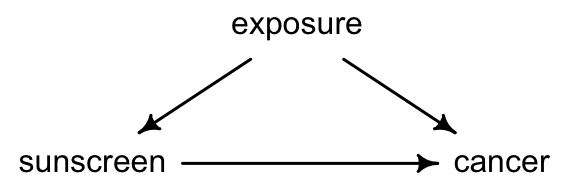
\includegraphics{Research-Design---Statistics_files/figure-latex/c4c11-1} 

}

\caption{DAG for effects of sunscreen use and sun exposure on skin cancer risk.}\label{fig:c4c11}
\end{figure}

If exposure increases the use of sunscreen and increases the risk of skin cancer, then that can generate an unexpected pattern of skin cancer being more common with sunscreen use! But let's say that sunscreen does have a direct causal effect of reducing skin cancer risk. If both forces are at play - the direct effect of sunscreen reducing cancer risk, and the confounding effect of sun exposure increasing sunscreen use and cancer risk - then you might not find any relationship at all between cancer risk and sunscreen use. In other words, sometimes confounders will \textbf{mask} a true causal effect, specifically if the pattern of the association between X and Y generated by the confounder is the opposite direction of the pattern of the association between X and Y generated by the direct effect.

\textbf{\emph{Identifying confounders on back-door paths:}} Confounders can be identified by finding \textbf{back-door paths} from the explanatory variable to the response variable. A back-door path is any path in the DAG that starts with an arrow pointing into the explanatory variable and ends with an arrow pointing into the response variable. Forks create backdoor paths: \(sunscreen \gets exposure \to cancer\).

Back-door paths can include more than two pathways. Consider a researcher trying to understand the causal effect of exercise on recovery time from a respiratory virus. Of course there are multiple potential common causes of exercise and viral recovery time. Figure \ref{fig:c4c12} shows a DAG that includes the expected causal effect of exercise on recovery time, but also general health knowledge and vaccination status. See if you can find the back-door path between exercise and recovery.

\begin{figure}

{\centering 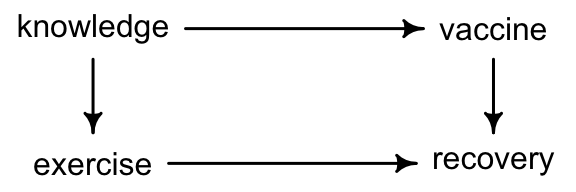
\includegraphics{Research-Design---Statistics_files/figure-latex/c4c12-1} 

}

\caption{DAG for causal effect of exercise on recovery time from a respiratory virus.}\label{fig:c4c12}
\end{figure}

The back-door path is \(exercise \gets knowledge \to vaccine \to recovery\). The confounder here is health knowledge. People with a lot of health knowledge might exercise more and be more likely to get vaccinated, and vaccination time can reduce recovery time. If that's the case, health knowledge confounds the relationship between exercise and recovery time. In this case, the back-door path includes more than one intervening node between the explanatory and response variable.

\textbf{\emph{Dealing with confounders:}} When there's a back-door path identified in a DAG that will confound the relationship between the explanatory and response variable, that pathway must be blocked or controlled. The options for blocking back-door paths involving confounders include study design and statistical analysis and will be addressed in coming chapters.

\subsection{The pipe: mediators}\label{the-pipe-mediators}

Let's continue examining the last DAG on viral recovery time to illustrate the next causal structure: the \textbf{pipe}. The pipe has a standard structure of \(X \to Z \to Y\). The variable Z is called a \textbf{mediator}, because the causal effect of X on Y is mediated (at least in part) by Z. You've probably noticed this structure in some of the DAGs we've explored so far. For example, the path \(knowledge \to exercise \to recovery\) is a pipe. Here, the causal effect of health knowledge is mediated by exercise. Essentially, the causal effect of knowledge is transmitted to viral recovery via exercise level. The path \(knowledge \to vaccine \to recovery\) is also a pipe. In this case, vaccination is a mediator transmitting the causal effect of knowledge to recovery.

When the causal effect of a variable X on Y involves a mediator Z, we call the causal effect of X on Y an \textbf{indirect effect}. A causal effect of X on Y can involve multiple indirect effects. Thus, one can examine the indirect effect of knowledge on recovery via exercise, or the indirect effect of knowledge on recovery via vaccination. Note that there is no direct effect of knowledge on recovery in this model.

Causal effects of a variable X on Y can also involve direct and indirect effects. Consider an ecologist asking whether the amount of forest habitat in a landscape causally affects bird species diversity. The researcher hypotheses that forest can affect species diversity in two ways. First, forest area can directly affect species diversity because the amount of forest affects the amount of resources available for birds (e.g., food, nesting sites). Second, forest area can indirectly affect species diversity by affecting the degree of habitat fragmentation. When forest area declines, the remaining forest becomes spatially fragmented, and fragmentation can have a direct effect on diversity by limiting the immigration of new species. Figure \ref{fig:c4c13} shows a DAG reflecting these ideas.

\begin{figure}

{\centering 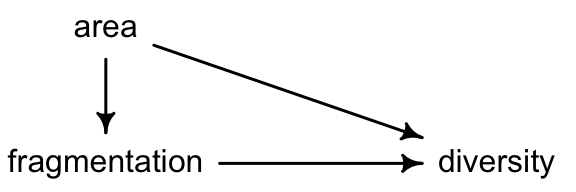
\includegraphics{Research-Design---Statistics_files/figure-latex/c4c13-1} 

}

\caption{DAG for causal effect of forest area and fragmentation on bird diversity.}\label{fig:c4c13}
\end{figure}

In this case, forest area has a direct effect on diversity and an indirect effect on diversity via the mediator fragmentation. The sum of a variables direct and indirect effects is called the \textbf{total effect}.

\textbf{\emph{Dealing with mediators:}} When the causal effect of X on Y involves a pipe, generally there is no need to do anything about the mediator. A mediator is an important component of the causal effect of the explanatory variable of interest. If I want to know the total effect of forest area on bird species diversity, then I should make sure that area can affect bird diversity in all the ways I hypothesize, including the direct effect and the indirect effect via fragmentation. If I block the effect of fragmentation on diversity as part of the research design or analysis, then I am blocking part of the causal effect of forest area on diversity. This is called \textbf{post-treatment bias}. The ``bias'' part of this phrase means that you would get the wrong answer if you wanted to know the total effect of area on diversity but blocked the effect of fragmentation. If you want to know either the total (or indirect effect) of a treatment variable (another term for an explanatory variable), then you need to let the causal effect of that treatment variable be transmitted through its mediators.

In some circumstances it is OK to block a mediators effect. For example, suppose I was specifically interested in the direct effect of forest area on bird diversity, independent of its effect via fragmentation. In that case, I would want to design the study or analysis in a way to block the pipe involving fragmentation, leaving only the direct effect of area on diversity.

\subsection{The inverted fork: colliders}\label{the-inverted-fork-colliders}

Imagine a researcher asks whether people who have serious illnesses (e.g., heart disease, cancer, autoimmune disorders) are more likely to be infected with COVID-19 than people who don't have serious illnesses. The researcher conducts the study by examining patient records from a local hospital and finds a surprising result: there's a \textbf{negative association} between serious illnesses and COVID-19. In other words, people who have serious illnesses appear \textbf{less} likely to have COVID-19 than those without a serious illnesses. But there's one problem with this analysis: it's not correct! Let's explore why with a simulated dataset.

Assume that serious illness status and COVID-19 status are binary categorical variables, and additionally assume that having a serious illness \textbf{increases} the probability of having COVID-19. Let's also assume that having a serious illness or COVID-19 increases the probability of someone being admitted to the hospital. Figure \ref{fig:c4c14} shows a DAG reflecting these assumptions.

\begin{figure}

{\centering 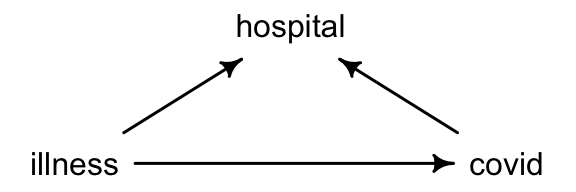
\includegraphics{Research-Design---Statistics_files/figure-latex/c4c14-1} 

}

\caption{DAG for the causal effect of serious illness on COVID infection status.}\label{fig:c4c14}
\end{figure}

And now here's the R code to generate some data based on the stated assumptions, using the \texttt{rbinom} function to simulate binary data just like in the example on greenspace and mental health outcomes.

\begin{Shaded}
\begin{Highlighting}[]
\FunctionTok{set.seed}\NormalTok{(}\DecValTok{123}\NormalTok{)}

\DocumentationTok{\#\# simulate illness status}
\NormalTok{ill }\OtherTok{\textless{}{-}} \FunctionTok{rbinom}\NormalTok{(}\AttributeTok{n =} \DecValTok{1000}\NormalTok{, }\AttributeTok{size =} \DecValTok{1}\NormalTok{, }\AttributeTok{prob =} \FloatTok{0.2}\NormalTok{)}

\DocumentationTok{\#\# simulate covid status based on illness status}
\NormalTok{cov }\OtherTok{\textless{}{-}} \FunctionTok{rbinom}\NormalTok{(}\AttributeTok{n =} \DecValTok{1000}\NormalTok{, }\AttributeTok{size =} \DecValTok{1}\NormalTok{, }\AttributeTok{prob =} \FunctionTok{ifelse}\NormalTok{(ill }\SpecialCharTok{==} \DecValTok{1}\NormalTok{, }\FloatTok{0.2}\NormalTok{, }\FloatTok{0.1}\NormalTok{))}

\DocumentationTok{\#\# simulate hospital status based on illness status and covid status}
\NormalTok{hos }\OtherTok{\textless{}{-}} \FunctionTok{rbinom}\NormalTok{(}\AttributeTok{n =} \DecValTok{1000}\NormalTok{, }\AttributeTok{size =} \DecValTok{1}\NormalTok{, }\AttributeTok{prob =} \FunctionTok{ifelse}\NormalTok{(ill }\SpecialCharTok{==} \DecValTok{1} \SpecialCharTok{\&}\NormalTok{ cov }\SpecialCharTok{==} \DecValTok{1}\NormalTok{, }\FloatTok{0.29}\NormalTok{, }
                                         \FunctionTok{ifelse}\NormalTok{(ill }\SpecialCharTok{==} \DecValTok{1} \SpecialCharTok{\&}\NormalTok{ cov }\SpecialCharTok{==} \DecValTok{0}\NormalTok{, }\FloatTok{0.25}\NormalTok{,}
                                         \FunctionTok{ifelse}\NormalTok{(ill }\SpecialCharTok{==} \DecValTok{0} \SpecialCharTok{\&}\NormalTok{ cov }\SpecialCharTok{==} \DecValTok{1}\NormalTok{, }\FloatTok{0.05}\NormalTok{, }\FloatTok{0.01}\NormalTok{))))}
\end{Highlighting}
\end{Shaded}

Here are the quantitative assumptions we've made in this simulated dataset of 1000 people:

\begin{enumerate}
\def\labelenumi{\arabic{enumi}.}
\tightlist
\item
  The baseline probability of someone having a serious illness is 20\%.
\item
  Serious illness increases the risk of COVID infection. The probability of a COVID infection is 20\% for those with a serious illness and 10\% for everyone else.
\item
  Serious illness and COVID both increase the chance of being admitted to the hospital. The baseline probability of someone without a serious illness or COVID being admitted to the hospital is assumed to be 1\%. A serious illness increases the risk by 24\%, and a COVID infection increases the risk by 4\%. Thus, if someone has COVID but no serious illness (\texttt{ill\ ==\ 0\ \&\ cov\ ==\ 1}), their chance of being in the hospital is 5\%. If someone has a serious illness but not COVID (\texttt{ill\ ==\ 1\ \&\ cov\ ==\ 0}), their chance of being in the hospital is 25\%. If someone has a serious illness and COVID (\texttt{ill\ ==\ 1\ \&\ cov\ ==\ 1}), their chance of being in the hospital is 29\%.
\end{enumerate}

Now let's replicate the researcher's analysis by filtering the dataset to only include hospitalized patients, and then we will examine the relationship between serious illness and COVID status:

\begin{Shaded}
\begin{Highlighting}[]
\NormalTok{d }\OtherTok{\textless{}{-}} \FunctionTok{cbind.data.frame}\NormalTok{(ill, cov, hos) }\CommentTok{\#create a data frame with all 3 variables}
\NormalTok{hos.patients }\OtherTok{\textless{}{-}}\NormalTok{ d[d}\SpecialCharTok{$}\NormalTok{hos }\SpecialCharTok{==} \DecValTok{1}\NormalTok{,] }\CommentTok{\#extract the observations for the hospital patients}

\FunctionTok{addmargins}\NormalTok{(}\FunctionTok{table}\NormalTok{(hos.patients}\SpecialCharTok{$}\NormalTok{ill, hos.patients}\SpecialCharTok{$}\NormalTok{cov,}
                 \AttributeTok{dnn =} \FunctionTok{c}\NormalTok{(}\StringTok{"ill"}\NormalTok{, }\StringTok{"cov"}\NormalTok{)))}
\end{Highlighting}
\end{Shaded}

\begin{verbatim}
##      cov
## ill    0  1 Sum
##   0    8  4  12
##   1   47 12  59
##   Sum 55 16  71
\end{verbatim}

From the filtered dataset, we can see that we have a total of 71 hospital records. Of the 71 patients, 47 patients have a serious illness but not COVID, 4 patients have COVID but not a serious illness, and 12 patients have a serious illness and COVID. Does having a serious illness increase the risk of COVID?

If we simply compute the probability of COVID for people with and without a serious illness, here's what we find. The probability of COVID is 12/59 = 20\% for people with a serious illness and 4/12 = 33\% for people without a serious illness. That's right. Among hospitalized patients, people without a serious illness appear more likely to have COVID than those with a serious illness, the opposite of the true relationship in the general population based on our simulated model.

This counterintuitive result arises from \textbf{collider bias}. Take another look at the DAG and note that both serious illness and COVID status causally affect hospital admission: \(Illness \to Hospital \gets COVID\). This causal structure is called an inverted fork: \(X \to Z \gets Y\), where the variable Z is called a \textbf{collider} because it is causally affected by both X and Y. Hospital admission is a collider, where a patient is most likely to be admitted if they have a serious illness or COVID.

\textbf{\emph{Dealing with colliders:}} Colliders only create problems when a researcher blocks or controls for the collider Z in the pathway \(X \to Z \gets Y\) as part of the research design or analysis. That's exactly what's happening with our example case of filtering the dataset to only individuals who were admitted to the hospital. When conditioning on hospital admissions in this way, a spurious relationship is generated between serious illness and COVID status.

Think about it this way. When we restrict the analysis to hospitalized patients, the two causes of hospitalization compete in a away to explain why patients were admitted. If a patient doesn't have COVID, they must have had a serious illness. If a patient doesn't have a seriuos illness, they must have had COVID. This creates a spurious negative relationship between serious illness and COVID status, even though the true relationship in the general population is just the opposite.

Collider bias is a type of \textbf{selection bias} in that it's driven by analyzing relationships between variables within a certain group. The world is full of these kind of examples. Why do ex-partners tend to either be attractive or intelligent, but not both? In this case the sample is restricted only to the people you dated in the past. If an ex wasn't particularly attractive, they were probably intelligent. If an ex wasn't intelligent, they were probably attarctive. Individuals who were neither attractive nor intelligent never made it into the pool of individuals you'd choose to go on a date with!

So beware of colliders. When you are interested in the causal relationship between X and Y, and X and Y both affect Z, generally avoid filtering the dataset by Z!

\section{Closing backdoor paths}\label{closing-backdoor-paths}

Drawing a DAG is a really useful way of being explicit about your scientific model, but it can also inform how you should go about designing your study and analyzing data. That's ultimately why we're covering graphical causal diagrams before we jump into statistics. DAGs represent your causal assumptions, and everything else - design, analysis, inference - follows from that. Science before statistics!

Once you have a DAG in hand, you can evaluate it to identify problematic pathways, basically any causal path that confounds the causal effect of interest. The causal pathways of interest start with a particular explanatory variable X and end with an outcome variable Y, and the arrows between X and Y should be forward facing. We will call these pathways \textbf{directed paths}, which are causal and of primary interest. This might involve a direct effect of X on Y, \(X \to Y\), indirect effects of X on Y \(X \to Z \to Y\), or both (the total effect). Problematic pathways are \textbf{back-door paths}, which are paths that connect X to Y but start with an arrow pointing into X. A fork structure with a confounder is the classic example. Back-door paths are noncausal and must be blocked. Finally, some paths between X and Y will start with a directed path out of X but end with a collider. If there's a collider on a pathway between X and Y, that pathway is noncausal but is already blocked. No further action is needed.

Let's take a look at an example. Figure \ref{fig:c4c17} shows a DAG where the interest is in understanding the causal effect of screen time on obesity in pediatric patients (\href{https://www.nature.com/articles/s41390-018-0071-3}{Williams et al.~2018}). The DAG includes three other relevant variables, parent education, physical activity, and self-harm. This DAG represents a scientific hypothesis about the causal relationship between screen time and obesity, but it also includes other relevant pathways that are noncausal but could generate a spurious association between screen time and obesity. To understand how best to proceed with the design and analysis phase of the research, one would start by listing all the pathways between screen time and obesity, then identify the causal pathways of interest and the noncausal pathways. Given a list of all the pathways, causal and noncausal, one can then determine if any action needs to be taken to block the noncausal pathways from generating spurious associations.

\begin{figure}

{\centering 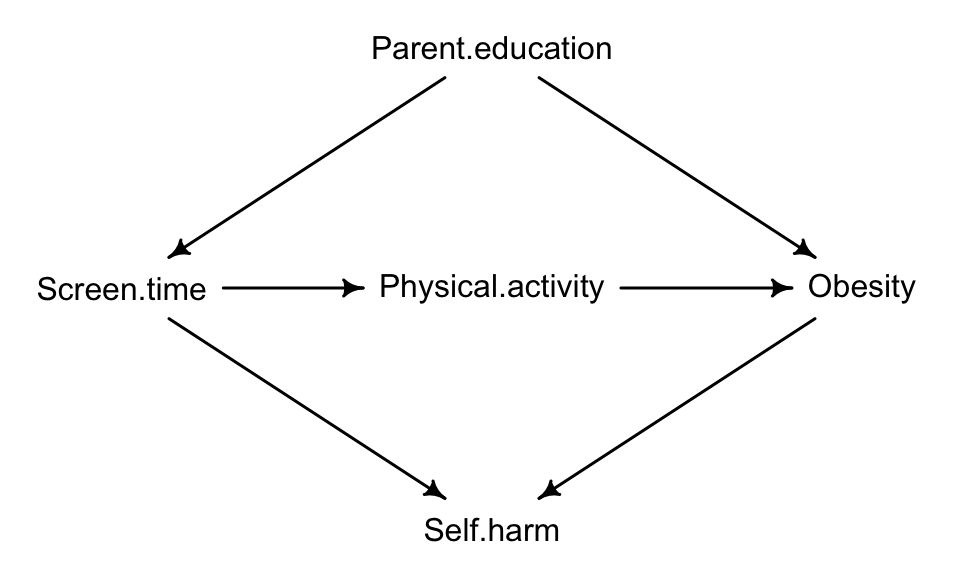
\includegraphics{Research-Design---Statistics_files/figure-latex/c4c17-1} 

}

\caption{DAG for the causal effect of screen time on obesity in pediatric patients.}\label{fig:c4c17}
\end{figure}

Below I list every path connecting the explanatory variable (screen time) to the response variable (obesity). For each path, we identify whether it is directed, back-door, or blocked via a collider. Given this information, one can decide which variables should be controlled during the design or analysis phase, and which variables should be left alone.

\begin{itemize}
\item
  \(Screen.time \to Physical.activity \to Obesity\): Here we have a pipe. This is a forward causal pathway involving an indirect effect of screen time on obesity via physical activity. The hypothesis here is that the more time a child spends on a screen, the less time they are being physically active, and the more likely they will be obese. This is a causal pathway of interest, so we wouldn't want to block it. It would be a mistake to block or condition on physical activity, because that's assumed to be an essential component of the causal mechanism linking screen to obesity. Blocking physical activity would be an example of post-treatment bias.
\item
  \(Screen.time \gets Parent.education \to Obesity\): This is a back-door path because it involves an arrow pointing into the explanatory variable. The causal structure is a fork, where parent education is a confounder. Thus, this is a non-causal path that will generate a spurious association between screen time and obesity. We need to block the effect of parent education on obesity during the design or analysis phase of the research.
\item
  \(Screen.time \to Self.harm \gets Obesity\): This is a path involving a collider. Note that both screen time and obesity are assumed to have direct effects on self-harm. Collider paths are blocked by default, so no action is necessary. It would be a mistake to design the research or conduct the analysis in a way that conditions on self-harm (for example, by only analyzing individuals who have a history of self-harm), because that would generate a noncausal association between screen time and obesity.
\end{itemize}

There you have it. With a DAG in hand, you can identify all the potential paths bewteen the explanatory and response variable, and determine for each whether not they need to be blocked. We will examine the methods of blocking available when we explore study designs and linear models later in the book.

\section{Like all models, DAGs require assumptions}\label{like-all-models-dags-require-assumptions}

The great value of using DAGs is that they make causal assumptions crystal clear. Based on those assumptions and the causal structures observed in a DAG, one can design a data colleciton scheme or analyze the data in a way that increases the chance of obtaining an unbiased estimate of the causal effect of interest. But like all models, DAGs are simplifications of nature and have their own assumptions. Here are some important ones:

\begin{enumerate}
\def\labelenumi{\arabic{enumi}.}
\item
  Causal effects in DAGs cannot be bidirectional. They must be \textbf{directed} from one variable to another.
\item
  DAGs cannot have cycles. In other words, you can't have a causal effect structure like this where you start with a causal effect of variable X and have a chain of causal effects that end back at X: \(X \to Y \to Z \to X\). Cycles or loops are not allowed. DAGs are most beneficial to represent static causal models. If your scientific hypothesis is more dynamic, involving time and feedback loops, other tools for causal inference will often be necessary.
\item
  All variables with non-trivial effects should be included. This is most important when two variables have a shared cause, like Z here: \(X \gets Z \to Y\). The reason it's important to include common causes is because such confoudners need to be blocked by design or in the analysis to get an unbiased estimate of the relationship between X and Y. Unobserved or unmeasured confounders will lead to biased conclusions, although there are methods to help address unobserved confounders.
\item
  Building on the previous point, using a DAG to inform research design and analysis does not magically make any association you find a causal relationship. Leaving non-trivial variables out of the DAG, particularly confounders, will make causal conclusions from the DAG invalid. Domain knowledge becomes extremely important when designing a DAG to ensure that it adequately represents prior knowledge about the science of the research question.
\end{enumerate}

So DAGs have assumptions and limits like any model, but they are a very useful method for an initial exploration of the tools of causal inference. We'll build on this foundation moving forward.

\chapter{Elements of Research Design: Study Type}\label{elements-of-research-design-study-type}

So far we have examined the importance of identifying a clear research question and communicating the causal assumptions related to the research question with a DAG. I've tried to make the case that defining clear research questions and developing an explicit scientific model as a DAG will help inform how one goes about designing research to collect and analyze data. In the next two chapters, we will begin to look at some basic elements of research design given a question and DAG in hand. We'll first explore our options for different types studies we can conduct, and then we'll explore the concept of sampling to collect data and some principles we can apply to maximize the quality of our dataset and the inferences we make from the data. Let's begin with study design.

\section{Types of Study Designs}\label{types-of-study-designs}

Consider the last research question from Chapter 4 on graphical causal models: Does screen time affect obesity in children? The hypothesis here is that screen time increases obesity due to reduced physical activity. Time is a zero sum game. Children who spend four hours on a screen each day are not spending those four hours being physically active, and increased risk of obesity may be a consequence of reduced physical activity. In the terms of a DAG in Figure \ref{fig:c5c1}, the expectation is that screen time indirectly increases obesity by reducing physical activity, where physical activity is a mediator.

\begin{figure}

{\centering 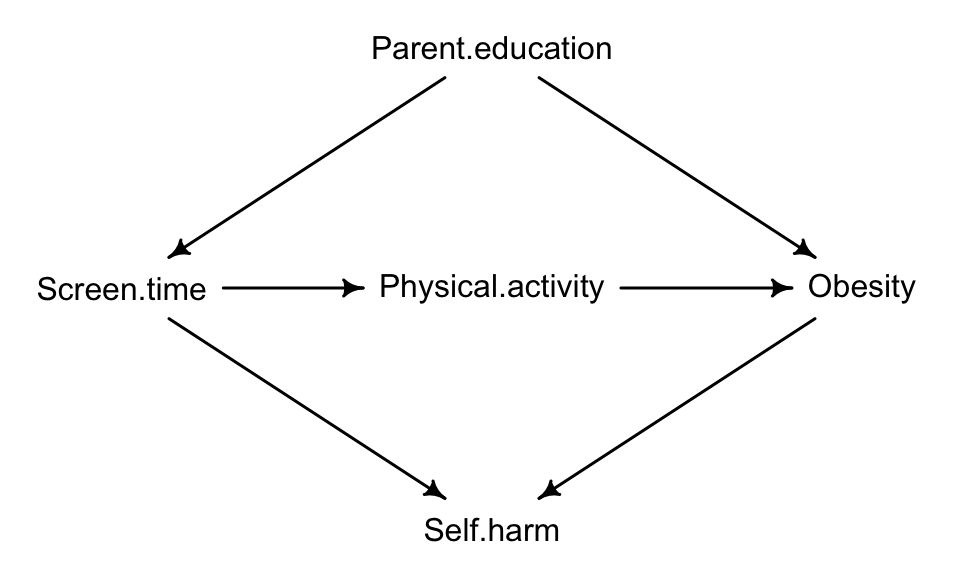
\includegraphics{Research-Design---Statistics_files/figure-latex/c5c1-1} 

}

\caption{DAG for the causal effect of screen time on obesity in pediatric patients.}\label{fig:c5c1}
\end{figure}

The DAG from Chapter 4 also includes two additional variables that are causally related the explanatory and response variable. Screen time and obesity are both expected to have direct effects on self-harm. Because self-harm is a collider in this DAG, and the path \(Screen.time \to Self.harm \gets Obesity\) is blocked by default. In other words, when we design the research, we should \textbf{not} attempt to do anything additionally in our research design to block the self-harm outcome. Doing so would actually create a noncausal association between screen time and obesity.

The other relevant path in the DAG is \(Screen.time \gets Parent.education \to Obesity\). This is a back-door path with a confounding effect of parent education. Here the idea is that parents with a lot of education about health will know something about the risks of screen time and the risks of obesity, and they may take actions to minimize screen time and obesity in their children through mechanisms other than physical activity. For example, perhaps the parents who restrict screen time are also likely to restrict their children's diet to the most health foods. If that were the case, you might find a positive association between obesity and screen time. But that positive association wouldn't reflect the causal effect of screen time.

Given this DAG and the potential confounding effect of parental education, how do we proceed to design the study? There are two general types of study designs we can use: experimental and observational research.

\section{Experimental studies}\label{experimental-studies}

\textbf{\emph{Experiments}} are essentially the gold standard for scientific research when the goal is causal explanation. There are two key elements of experiments. First, the researcher manipulates the explanatory variable. In other words, individuals in the experiment are assigned particular values of the explanatory variable, often referred to as the \textbf{treatment}. Second, the particular values of the explanatory varaible are \textbf{randomly assigned} to individuals in the experiment. This element is called \textbf{randomization}, and it is really the defining feature of an experiment.

Why is randomization so important? Let's consider this question in the context of the research question on screen time and obesity. The DAG shows that parent education is a confounding variable. Thus, the concern is that kids who have low levels of screen time have parents with high levels of education, and those parents with high education parent in other ways (besides screen time) to minimize the chance that their kids will be obese. If the researcher is interested in the effect of screen time on obesity, then the confounding effect of parent education must be controlled. And that's what randomization does.

Suppose the researcher enrolls 200 kids into the study. The researcher decides that she will assign three possible levels of screen time: 0, 5, or 10 hours per week. These different levels of screen time will be assigned to each participant randomly. For example, the researcher might have a list of each individual's name (or more likely, an identification code), and for each individual she could pick a piece of paper out of a hat indicating one of the three treatment levels. Or, she can use 21st-century technology and assign one of the three treatment levels in R:

\begin{Shaded}
\begin{Highlighting}[]
\FunctionTok{set.seed}\NormalTok{(}\DecValTok{123}\NormalTok{)}
\DocumentationTok{\#\# create ID codes for each participant}
\NormalTok{id }\OtherTok{\textless{}{-}} \DecValTok{1}\SpecialCharTok{:}\DecValTok{200}

\DocumentationTok{\#\# define the three treatment levels (0 = none, 5 = low, 10 = high)}
\NormalTok{trt.levels }\OtherTok{\textless{}{-}} \FunctionTok{c}\NormalTok{(}\StringTok{"none"}\NormalTok{, }\StringTok{"low"}\NormalTok{, }\StringTok{"high"}\NormalTok{)}

\DocumentationTok{\#\# randomly assign each individual to a treatment}
\NormalTok{trt }\OtherTok{\textless{}{-}} \FunctionTok{sample}\NormalTok{(trt.levels, }\DecValTok{200}\NormalTok{, }\AttributeTok{replace =} \ConstantTok{TRUE}\NormalTok{)}

\DocumentationTok{\#\# combine into a dataframe}
\NormalTok{d }\OtherTok{\textless{}{-}} \FunctionTok{cbind.data.frame}\NormalTok{(id, trt)}
\FunctionTok{head}\NormalTok{(d)}
\end{Highlighting}
\end{Shaded}

\begin{verbatim}
##   id  trt
## 1  1 high
## 2  2 high
## 3  3 high
## 4  4  low
## 5  5 high
## 6  6  low
\end{verbatim}

The \texttt{sample} function was used to randomly assign each of the 200 participants to one of the three treatment levels \footnote{The \texttt{replace} = TRUE argument just means that the sampling is done ``with replacement''. That means if the first person is assigned the ``high'' treatment, the next person can also be assigned the ``high'' treatment.}. Here's why randomization is the key feature of an experiment: If the treatment levels are randomly assigned to each individual, then there will be no relationship between the screen time of each participant and their parent's education level. A participant with who has highly educated parents will have an equal chance of being assigned to each of the three levels of screen time. In other words, experiments remove the influence of confounding variables on the explanatory variable. If the researcher used an experiment in this way, the DAG would be revised to eliminate the \(Parent.education \to Screen.time\) effect as seen in Figure \ref{fig:c5c3}.

\begin{figure}

{\centering 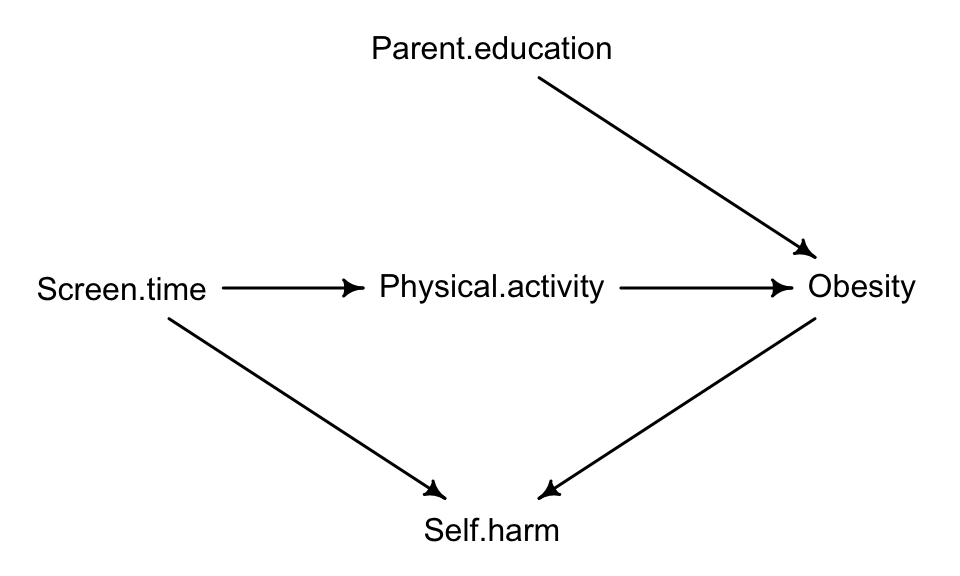
\includegraphics{Research-Design---Statistics_files/figure-latex/c5c3-1} 

}

\caption{DAG for the causal effect of screen time on obesity in pediatric patients when using an experimental study design.}\label{fig:c5c3}
\end{figure}

In this revised DAG, there is no longer a back-door path confounding the relationship between screen time and obesity. The research would randomly assign the levels of screen time, let enough time pass to observe the expected effect, and then record the value of the outcome variable, obesity (likely as the change in obesity from the start to the end of the study).

Random assignment of the explanatory varaible to individuals in an experiment not only helps control for confounding variables the researcher is aware of, but also unobserved confounders. Even with extensive domain knowledge, it's hard to think about every possible confounding variable and to include each one in the DAG. Randomization breaks the association between the explanatory varaible and unobserved confounders too.

Experiments are sometimes referred to as \textbf{randomized controlled trials (RCTs)}, emphasizing the essential component of randomization when attempting to infer a causal effect of an explanatory variable. The ``controlled'' part of the RCT name often refers to a \textbf{control group}, which is a group that does not receive the standard treatment. Control groups are often essential as a baseline for comparison. In the experiment described here on screen time and obesity, the ``none'' category of screen time is the control group. However, experiments don't always need a control group as traditionally defined. For example, suppose that instead of ``none'', ``low'', and ``high'', we just dropped the ``none'' category and assigned individuals to one of two treatment levels: low and high screen time. The researcher would still randomly assign these two levels of screen time to participants and then compare the change in obesity between the two groups. The ``low'' treatment functions as the baseline for comparison. A researcher might not include a traditional control group (complete absence of the treatment) if that's not a realistic value in the target population of interest, such as if the study is being conducted on a population where virtually no children have exactly zero screen time.

Although experiments are the goal standard of causal inference, correct causal inference isn't a guarantee. One problem researchers face is when participants in an experiment don't comply with their treatment instructions. This kind of issue can be common in experiments requiring behavioral compliance of people (e.g., psychology; \href{https://compass.onlinelibrary.wiley.com/doi/epdf/10.1111/spc3.12948}{Rohrer 2023}). For example, imagine that some individuals who were assigned to the ``none'' treatment still give their kids some screen time. When compliance is a potential issue, researchers should collect data on both the treatment level randomly assigned \emph{and} the treatment level actually received. Hopefully participatns are honest, and the person assigned to the ``none'' treatment level reports their actual screen time.

But even if people are honest and report their actual screen time, the noncompliance introduces significant complication for the analysis. Although the treatment levels were randomly assigned to participants, the noncompliance may not be random. What if noncompliance is affected by parental education? In this case, perhaps the most highly educated parents enforce stricter screen time limitations than the treatment they were assigned, where as parents with less education may be more likely to relax a strict limitation and allow their kids to have more screen time. The DAG in Figure \ref{fig:c5c4} below is modified to reflect this possibility, now including a variable for the actual screen time experienced by the participants, and a direct causal effect of parent education on actual screen time. The researcher might have been aware of noncompliance and collected data on \emph{actual} screen time, but it would be a mistake to simply analyze the relationship between obesity and actual screen time. Why? There's a backdoor path from actual screen time to obesity via the confounder, parent education. Even in an experimental context, correctly analyzing the causal effect of screen time in this example would require an analysis that controls for the effect of parental education on actual screen time.

\begin{figure}

{\centering 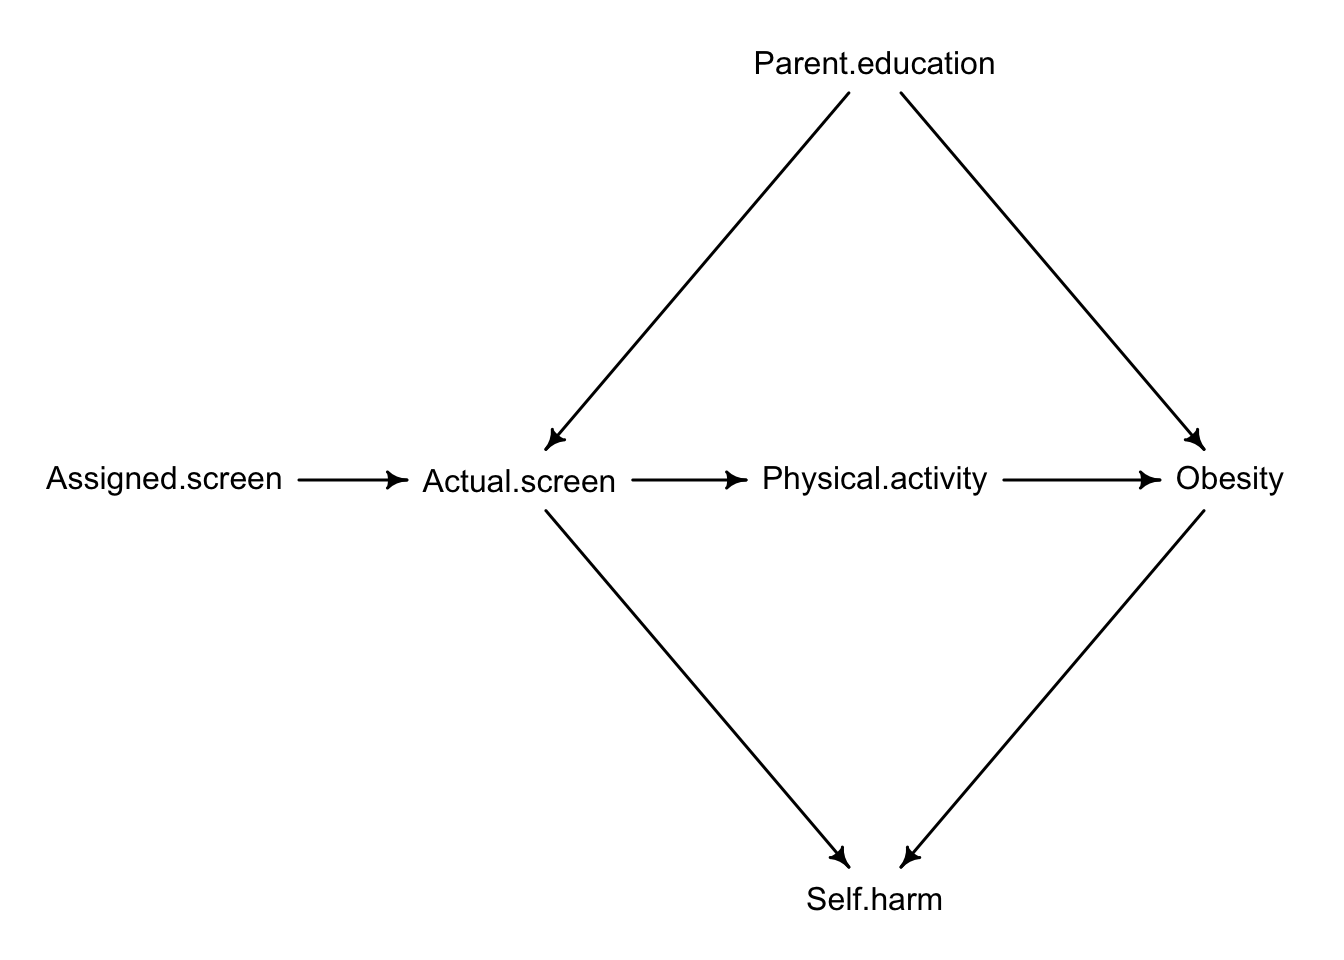
\includegraphics{Research-Design---Statistics_files/figure-latex/c5c4-1} 

}

\caption{Revised DAG including actual screen time.}\label{fig:c5c4}
\end{figure}

So, experiments aren't a guarantee of safe causal inference, even when treatments are randomly assigned. Moreover, sometimes conducting experiments can be challenging, or even impossible. Imagine you're an economist studying the effect of the minimum wage on employment. It's impossible to randomly assign different minimum wages to different municipalities. If you're a biologist studying the effect of urbanization on biodiversity, you can't randomly assign areas that do and do not become urbanized. Sometimes experiments can't be done because they're unethical. If you're a psychologist studying the effect of parenting style and child personality, you can't randomly assign babies to different parenting styles. In cases like these, researchers have to rely on observational designs, which we turn to next.

\section{Observational studies}\label{observational-studies}

When researchers collect data without randomly assigning levels of the explanatory variable to individuals, they are conducting an \textbf{\emph{observational study}}. The key element making a study observational is when the researcher has no role in determining how the data arose. The data arose naturally and are observed and recorded by the reseacher. Sometimes you have to take what you can get.

How would an observational design be conducted to address our research question on screen time and obesity. There's a couple ways such a study could proceed. One approach would be to enroll individuals into a study and track their screen time and obesity over time. This kind of design is called a \textbf{prospective study}, which is simply a study that is planned in advance. Another approach would be to analyze existing data on screen time and obesity. Perhaps a dataset was previously collected by these factors by another researcher, or by a medical doctor in their own practice. This kind of design is called a \textbf{retrospective study}, referring to the fact that the data being analyzed were generated in the past. Both of these designs have the common element of the data arising naturally on their own without the researcher randomly assigning levels of screen time.

In some ways observational studies are much easier to pull off, particularly if a dataset is already available. But observational designs can present significant challenges in interpretation. Because the levels of the explanatory variable are not randomly assigned, any back-door path involving a confounding variable is unblocked in an observational design. Sure, it might be easy to record screen time and obesity for a bunch of kids, but remember parental education? Kids that have knowledgeable parents might limit their screentime and enforce a diet that minimizes obesity. In that case, one would find a positive relationship between screen time and obesity, not because of a causal effect of screen time, but because of confounding effect of parental education. This is exactly what people mean when they say ``correlation is not necessarily causation''. In addition to generating noncausal correlations, it's also important to remember that confounders can also mask real relationships.

So how do we proceed to make causal inferences with an observational design? One needs to have a clear scientific model of their system that makes causal assumptions clear, such as with a DAG. With a well-defined DAG that identifies likely back-door paths and confounders, one can then block those paths during the analysis phase. We won't learn the methods to do that until later in the book, but at this point it's important to understand that the researcher must identify potential confounders \emph{and} measure them in order to apply the methods we'll use to block back-door paths during analysis. That's why researchers should start by defining a DAG before the data are collected.

\subsection{Pros and cons of prospective vs.~retrospective studies (planned)}\label{pros-and-cons-of-prospective-vs.-retrospective-studies-planned}

\chapter{Elements of Research Design: Sampling Strategies}\label{elements-of-research-design-sampling-strategies}

At this point we know that effective research practice requires articulating a clear question, identifying causal assumptions about the relationship between response and explanatory variables, and proceeding with an experimental or observational study design. Once these issues are settled, it's time to think about data collection. But don't go so fast! The way in which one collects data goes a long way in determining the quality of data analysis and the uncertainty about our conclusions. In this chapter, we will take a close look at how data should be collected in a way that maximizes the quality of our data and minimizes the uncertainty in our conclusions.

\section{Inferences from data are (almost) always uncertain}\label{inferences-from-data-are-almost-always-uncertain}

I teach a statistics class as part of a biology curriculum, so the students in my class are either majoring in biology or something else. What proportion of the students in my class are biology majors? Hey - that's a research question! On it's own, it's not a very interesting research question, as it is purely descriptive. But for a variety of reasons, it is useful to know something about the background of students taking a course.

Notice that my question is very specific about \emph{who} I want to make conclusions about. What proportion of the students in \emph{my class} are biology majors? This is an example of a research question that is very limited in scope. In a typical semester, I have about 24 students in my statistics class. For my research question, those 24 students represent the \textbf{population} of interest. The target population is very specific and small.

Now suppose my research question is \emph{What proportion of all students taking a statistics class are biology majors?}. Now things are more complex. This research question is still descriptive - I simply want to know the value of a proportion - but now the scope is much broader. The statistical population for this question is now everyone who is taking a statistics class at the moment. Everyone where? Presumably everyone who is taking a statistics class at a university where a biology major is offered. Although notice that one could address this question for students taking a statistics class anywhere, whether or not there's a biology major offering. And what about the temporal scope of the question? Is it all students taking a statistics class \emph{right now}, over the last 5 years, or some other temporal scope? Remember that the population is basically the who, what, when, and where of your research question, and often it requires more detailed information beyond a simple one-sentence statement of the research question.

When the target population is very limited in scope, the design, analysis, and conclusions are often straightforward. Why? Well, it's not too hard to track down every student in my class of 24 and ask whether or not they are a biology major. In fact, I can just log onto my university's academic management system and obtain a record of the declared major of each student in the class. If 16 students are listed as biology majors and 8 students are not biology majors, then the proportion of biology majors in my class is simply 16/24 = 0.8 (80\%). I can answer my research question with virtual certainty, mainly because my target population is so limited in scope. Now I wouldn't say that I'm \emph{completely} certain that exactly 80\% of the students in my class are biology majors. Why not? There are a number of reasons. It's possible that the records are not all correct. It's possible that someone is classified as a biology major by mistake. Or maybe a student dropped the class, but that wasn't updated in the records at the time I retrieved the data. In other words, even when the target population is limited, there's almost always some sources of uncertainty.

Usually there's more uncertainty as the target population of inference grows larger. Let's say I'm interested in the proportion of biology majors taking a statistics class this semester in North American universities. I've narrowed down the scope of the research question pretty well, and therefore I have a good sense of the who, what, when, and where I can generalize about based on my study. But now I'm faced with the challenge of collecting data in a way that adequately represents a very large population of interest. If I want to know the proportion of biology majors with the same degree of confidence that I had when I was focused only on my particular class, I'd have to track down every single statistics class in North American universities and then determine whether each student is a biology major or not. That's not going to happen. Logistically it is simply impossible to collect data from everyone in the population in this case.

This is basically the crux of the problem of why we need the field of statistics. We need statistics because most research questions involve populations that are too large to collect data from in their entirety. When the population is too big, we need to take a \textbf{sample} of individuals from the population to address the question. I can't track down every single statistics class, so instead I take a sample of statistics classes currently being offered and use that sample to \textbf{estimate} the proportion of biology majors. When I take a sample of statistics classes, inevitably there is going to be a difference between the proportion of biology majors that I estimate from the sample and the actual proportion of biology majors among all students taking statistics. And to the add to the problem, I'm still going to have to deal with some uncertainty about my measurements of the individuals that were included in my sample.

\section{Sampling requires estimation}\label{sampling-requires-estimation}

Consider a very simple case of coin flipping. With a fair coin, the probability of a coin landing on heads is 0.5. But let's just suppose you didn't know the probability of the coin landing on heads is 0.5. You're going to estimate the probability of the coin landing on heads through a process of sampling from 10 coin flips, recording the total number of heads out of the 10 flips. Is it possible to get 6 out of 10 heads, leading to 0.6 for the \textbf{estimated} probability of heads? Absolutely. Or you might get 3 out of 10 heads for an estimate of 3/10 = 0.3, or 5 out of 10 heads for an estimate of of 5/10 = 0.5. This is the problem of sampling - there will often be some variation between the estimate of the quantity of interest and the true value. That introduces uncertainty. If there's some error on my process of recording the outcome of each coin flip, then there will be even more uncertainty.

Let me show you exactly what I mean by simulating this exact situation. When we flip a coin, there are two possible outcomes, heads and tails. In other words, the variable in this case is categorical, and specifically it is binary because there are two possible outcomes. When we flip a coin 10 times, we can keep track of the number of heads (or tails - it doesn't matter), which will be anywhere from 0 to 10 heads. This process of counting the outcome of a binary variable across multiple trials is called a binomial function. Recall we can use the \texttt{rbinom} function to simulate sampling for a binary process:

\begin{Shaded}
\begin{Highlighting}[]
\DocumentationTok{\#\# flip a single coin (size = 1) 10 times (n = 10); the coin is fair (prob = 0.5)}
\FunctionTok{rbinom}\NormalTok{(}\AttributeTok{n =} \DecValTok{10}\NormalTok{, }\AttributeTok{size =} \DecValTok{1}\NormalTok{, }\AttributeTok{prob =} \FloatTok{0.5}\NormalTok{)}
\end{Highlighting}
\end{Shaded}

\begin{verbatim}
##  [1] 1 1 1 1 0 0 0 1 1 0
\end{verbatim}

In this case the function returns a vector of 1s and 0s. Let's define heads as 1 and tails as 0. In the simulation, the number of heads can be obtained by simply summing the number of 1s. Alternatively, we can define the arguments of the \texttt{rbinom} function to count the number of heads (1s) out of a single set of 10 flips:

\begin{Shaded}
\begin{Highlighting}[]
\DocumentationTok{\#\# flip a single coin (size = 1) 10 times (n = 10); the coin is fair (prob = 0.5)}
\FunctionTok{rbinom}\NormalTok{(}\AttributeTok{n =} \DecValTok{1}\NormalTok{, }\AttributeTok{size =} \DecValTok{10}\NormalTok{, }\AttributeTok{prob =} \FloatTok{0.5}\NormalTok{)}
\end{Highlighting}
\end{Shaded}

\begin{verbatim}
## [1] 3
\end{verbatim}

Cool. This isn't rocket science. Clearly you can flip a coin 10 times and count the number of heads without R, and intuitively you know that you won't always get exactly 5 heads out of 10 flips of a fair coin. But when we flip a coin 10 times, how often will we get 5 heads, or 4 heads, or 8 heads? You could flip a coin 10 times, count the number of heads, and repeat that process many times to get a sense of the relative frequency of the outcomes. But that will take you a long time! This is where we can harness the power of R. Let's simulate our coin flipping process of counting the number of heads out of 10 flips a total of 1 million times:

\begin{Shaded}
\begin{Highlighting}[]
\DocumentationTok{\#\# flip a single coin (size = 1) 10 times (n = 10); the coin is fair (prob = 0.5)}
\NormalTok{heads }\OtherTok{\textless{}{-}} \FunctionTok{rbinom}\NormalTok{(}\AttributeTok{n =} \DecValTok{1000000}\NormalTok{, }\AttributeTok{size =} \DecValTok{10}\NormalTok{, }\AttributeTok{prob =} \FloatTok{0.5}\NormalTok{)}
\NormalTok{heads[}\DecValTok{1}\SpecialCharTok{:}\DecValTok{20}\NormalTok{]}
\end{Highlighting}
\end{Shaded}

\begin{verbatim}
##  [1] 3 6 6 8 5 3 6 6 3 5 4 3 5 3 4 2 6 4 3 3
\end{verbatim}

Now we get a vector of 1 million observations, each recording the number of heads out of 10 flips. I'm showing you only the first 20 outcomes, but we can easily generate a table or graph to show the relative frequency of each outcome. Here are tables of the absolute count of each outcome, as well the probability of each outcome:

\begin{Shaded}
\begin{Highlighting}[]
\DocumentationTok{\#\# absolute count of outcomes}
\FunctionTok{table}\NormalTok{(heads)}
\end{Highlighting}
\end{Shaded}

\begin{verbatim}
## heads
##      0      1      2      3      4      5      6      7      8      9     10 
##    992   9712  44120 117823 204979 246133 204423 117305  43790   9723   1000
\end{verbatim}

\begin{Shaded}
\begin{Highlighting}[]
\DocumentationTok{\#\# probability (relative frequency) of outcomes}
\FunctionTok{prop.table}\NormalTok{(}\FunctionTok{table}\NormalTok{(heads))}
\end{Highlighting}
\end{Shaded}

\begin{verbatim}
## heads
##        0        1        2        3        4        5        6        7        8        9 
## 0.000992 0.009712 0.044120 0.117823 0.204979 0.246133 0.204423 0.117305 0.043790 0.009723 
##       10 
## 0.001000
\end{verbatim}

Figure \ref{fig:c6c5} shows a graphical view of the probability of each outcome.

\begin{Shaded}
\begin{Highlighting}[]
\FunctionTok{barplot}\NormalTok{(}\FunctionTok{prop.table}\NormalTok{(}\FunctionTok{table}\NormalTok{(heads)),}
        \AttributeTok{names.arg =} \FunctionTok{c}\NormalTok{(}\DecValTok{0}\SpecialCharTok{:}\DecValTok{10}\NormalTok{),}
        \AttributeTok{ylim=}\FunctionTok{c}\NormalTok{(}\DecValTok{0}\NormalTok{, }\FloatTok{0.25}\NormalTok{),}
        \AttributeTok{xlab =} \StringTok{"Number of Heads"}\NormalTok{, }\AttributeTok{ylab =} \StringTok{"Probability"}\NormalTok{,}
        \AttributeTok{col =} \StringTok{"skyblue"}\NormalTok{)}
\end{Highlighting}
\end{Shaded}

\begin{figure}
\centering
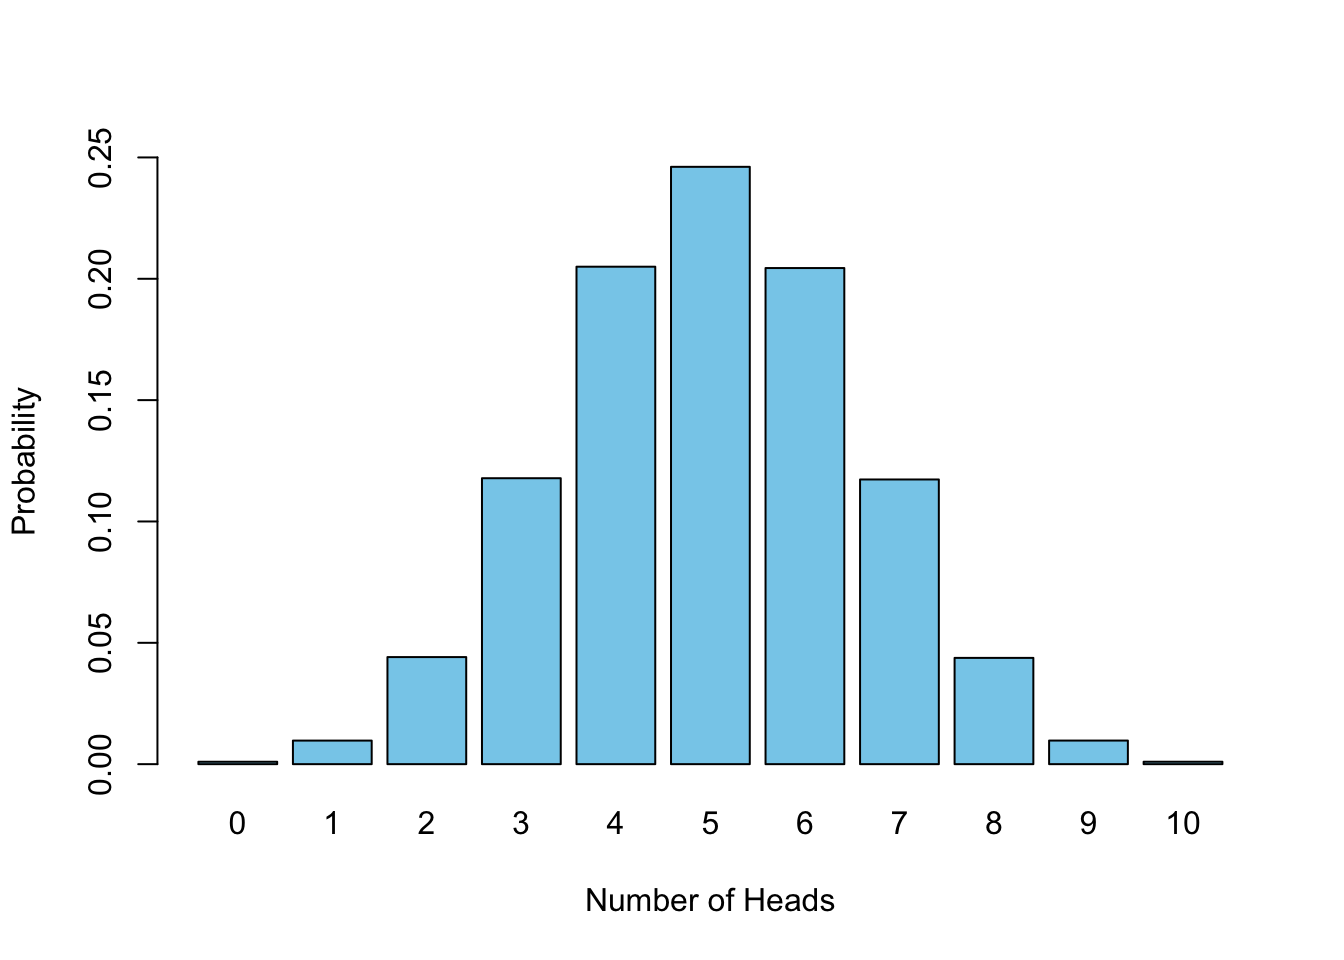
\includegraphics{Research-Design---Statistics_files/figure-latex/c6c5-1.pdf}
\caption{\label{fig:c6c5}Probability distribution of the number of heads out of 10 when repeating the sampling process one million times.}
\end{figure}

I like the graphical view. You can clearly see that getting five heads out of 10 is the most common outcome, but note that this outcome only happens about 25\% of the time. About 75\% of the trials result in an outcome other than five. If we didn't truly know we had a fair coin and we were estimating the probaiblity of heads by flipping the coin 10 times, there would be a difference between our estimate and the true value 75\% of the time. In other words, our estimates are just that - \textbf{estimates}. There is always uncertainty about the quality of an estimate, or how close it is to the truth.

Statistics is fundamentally about how to use data to estimate quantities of interest from samples \textbf{and the uncertainty about those estimates}. If I take a sample of 100 statistics courses and and 20\% of the students in those courses are biology majors, I can't conclude with certainty that the proportion of biology majors is really 0.2. The essential goal of statistics is to not only estimate a quantity of interest from data, but to also estimate the uncertainty about the estimate. We will examine tools that allow us to describe our confidence about the quantities we're trying to estimate. The true proportion of biology majors is very unlikely to be exactly 0.2, but I might be quite confident that it's between 0.15 and 0.25. How confident? Stay tuned.

One of the most significant challenges as scientist faces is how to make decisions about hypotheses in light of uncertainty. Let's say you take a sample of individuals to study the relationship between screen time and cognitive performance in kids, and you find that the kids who spend more time on screens tend to show lower cognitive performance. In your analysis of the data from this study, there is some quantity, or set of quantities, that you have estimated from the sample that indicates this negative association. How certain are you about those estimates? If your estimates are highly uncertain, then your ability to make a firm conclusion about the research question and hypotheses is going to be limited. But better to know about that limitation than to ignore it! Ultimately statistics helps us make decisions about hypotheses with data in light of uncertainty, and I hope to illustrate that idea throughout the book.

\section{Parameters and estimates and estimands, oh my!}\label{parameters-and-estimates-and-estimands-oh-my}

Like most technical disciplines, statistics is full of jargon. Sorry. Let's define some key terms related to sampling. Statistical analysis involves estimating the unknown from sample data. Consider again my goal of estimating the proportion of students in statistics classes that are biology majors. That proportion is unknown. Quantities with unknown values are called \textbf{parameters}. In my example, the parameter is the true proportion of statistics students majoring in biology. The parameter is a probability in this case, but parameters can be means, variances, rates, components of a complex statistical model, or any number of other quantities. The defining feature of parameters is that they are unknown and require estimation to answer your research question. If I collect data on 1000 statistics students and find that 123 are biology majors, then my \textbf{estimate} is 123/1000 = 0.123 for the proportion majoring in biology. Much of this class is about generating estimates (and characterizing their uncertainty) for parameters based on data we collect from samples.

Now, sometimes we have to estimate multiple parameters in a statistical analysis, but not all of the parameters are of direct interest for our research question. The quantities of interest for our reserach question are called \textbf{estimands} \footnote{See \href{https://journals.sagepub.com/doi/abs/10.1177/00031224211004187?journalCode=asra}{Lundberg et al.~2021} for an excellent overview of estimands.}. In my example on the proportion of students majoring biology, the question and analysis is so simple that there's only a single parameter, and it's the parameter I'm interested in. The true proportion of statistics students majoring in biology is the estimand. In a more complex statistical analyses, we will often have to estimate multiple parameters, but not every parameter is of interest. In other words, not every parameter is an estimand. For example, suppose I'm interested in how the amount of time students spend studying affects their grade on an exam. To address a question like that, we could build a regression model - which we will cover in this book - that includes many parameters, but only one of those parameters might be the estimand, representing the causal effect of study time on exam grades. In these cases of complex statistical analyses, it will be important to identify which parameters you're estimating are estimands, which is ultimately based on your research question.

When we estimate quantities from a sample, there's uncertainty about the quality of that estimate - how consistent it is, and how close to the truth it is. Fortunately there are ways to characterize the quality of our estimates and to estimate the uncertainty we have about our estimates. We'll look at different ways of characterizing the quality of an estimate first.

\section{Quality of estimates: accuracy and precision}\label{quality-of-estimates-accuracy-and-precision}

When we estimate quantities from a sample, there's uncertainty about the quantity of that estimate. We will explore two different ways of characterizing the quality of an estimate: how close our estimate should be to the truth based on our sampling design, and the variation in the possible values of the estimate we might obtain based on our sampling design. These two concepts are referred to as \textbf{accuracy} and \textbf{precision}, and estimates are of highest quality when they are both accurate and precise. Let's break these terms down.

\subsection{Accuracy}\label{accuracy}

On average, how close is an estimate from the truth? Let's reconsider our coin flipping problem to estimate the probability of heads. In this case we know we have a fair coin, and so the probaiblity of heads is 0.5, but imagine we didn't know that. Our sampling process consisted of flipping a coin 10 times and recording the number of heads. In this case, the parameter (and estimand) is the true probability of heads, and the estimate is the probability of heads computed from our sample data. If we record 8 heads out of 10 flips, our estimate for the probability of heads is 8/10 = 0.8. On its face, that particular estimate doesn't appear to be very accurate. The estimate is too high. However, take another look at the entire distribution of possible outcomes when we flip a coin 10 times, which we created with a simulation. Let's express the distribution on the scale of probability for the outcome, rather than the number of heads out of 10 (\ref{fig:c6c6}.

\begin{Shaded}
\begin{Highlighting}[]
\NormalTok{possible.estimates }\OtherTok{\textless{}{-}} \FunctionTok{seq}\NormalTok{(}\DecValTok{0}\NormalTok{, }\DecValTok{1}\NormalTok{, }\AttributeTok{by =} \FloatTok{0.1}\NormalTok{)}
\FunctionTok{barplot}\NormalTok{(}\FunctionTok{prop.table}\NormalTok{(}\FunctionTok{table}\NormalTok{(heads)),}
        \AttributeTok{names.arg =}\NormalTok{ possible.estimates,}
        \AttributeTok{ylim=}\FunctionTok{c}\NormalTok{(}\DecValTok{0}\NormalTok{, }\FloatTok{0.28}\NormalTok{),}
        \AttributeTok{xlab =} \StringTok{"Estimated probability of heads"}\NormalTok{, }\AttributeTok{ylab =} \StringTok{"Probability"}\NormalTok{,}
        \AttributeTok{main =} \StringTok{""}\NormalTok{,}
        \AttributeTok{col =} \FunctionTok{c}\NormalTok{(}\FunctionTok{rep}\NormalTok{(}\StringTok{"gray"}\NormalTok{, }\DecValTok{5}\NormalTok{), }\StringTok{"skyblue"}\NormalTok{, }\FunctionTok{rep}\NormalTok{(}\StringTok{"gray"}\NormalTok{, }\DecValTok{5}\NormalTok{)))}
\end{Highlighting}
\end{Shaded}

\begin{figure}
\centering
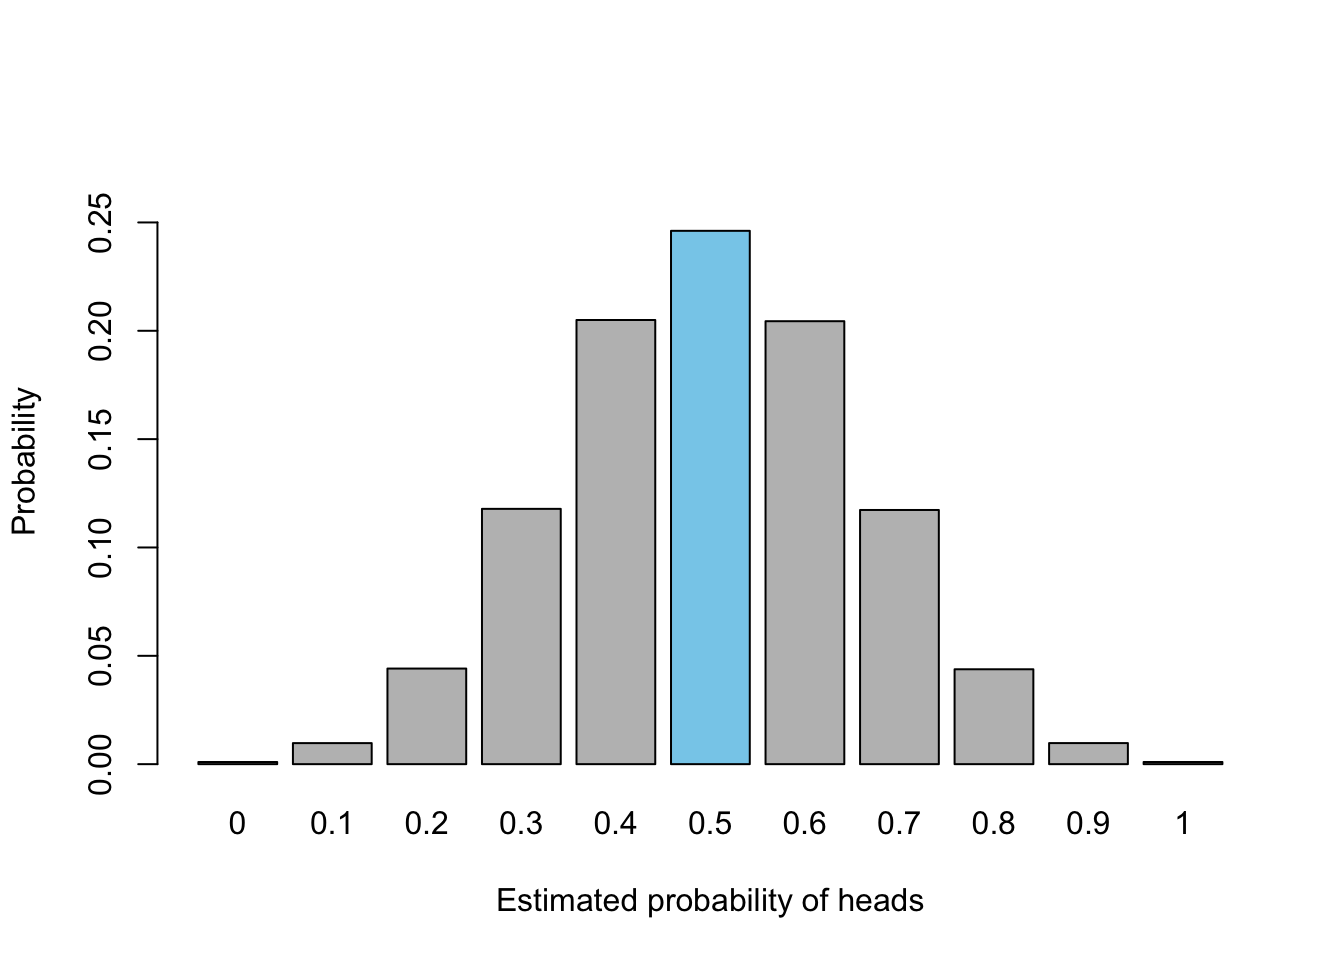
\includegraphics{Research-Design---Statistics_files/figure-latex/c6c6-1.pdf}
\caption{\label{fig:c6c6}Sampling distribution showing accuracy of estimates.}
\end{figure}

Notice that the most likely outcome based on our sampling process is 0.5 (highlighted in blue), which is exactly what the truth is. In other words, when considering our sampling process, repeatedly conducted many times, we get a sense for the entire distribution of possible estimates, and we see that our estimate is - \emph{on average} - accurate. Any particular estimate can be low or high, but there is no systematic difference between the estimate and the truth.

This distribution of possible outcomes of an estimate based on our sampling process is called a \textbf{sampling distribution}. If the sampling distribution is centered on the true value of a parameter, then your estimates are accurate. Figure \ref{fig:c6c7} shows one example of what a sampling distribution might look like when your estimate is not accurate:

\begin{Shaded}
\begin{Highlighting}[]
\DocumentationTok{\#\# generate a biased sampling distribution}
\NormalTok{heads.biased }\OtherTok{\textless{}{-}} \FunctionTok{rbinom}\NormalTok{(}\AttributeTok{n =} \DecValTok{1000000}\NormalTok{, }\AttributeTok{size =} \DecValTok{10}\NormalTok{, }\AttributeTok{prob =} \FloatTok{0.3}\NormalTok{)}
      
\NormalTok{possible.estimates }\OtherTok{\textless{}{-}} \FunctionTok{seq}\NormalTok{(}\DecValTok{0}\NormalTok{, }\DecValTok{1}\NormalTok{, }\AttributeTok{by =} \FloatTok{0.1}\NormalTok{)}
\FunctionTok{barplot}\NormalTok{(}\FunctionTok{prop.table}\NormalTok{(}\FunctionTok{table}\NormalTok{(heads.biased)),}
        \AttributeTok{names.arg =}\NormalTok{ possible.estimates,}
        \AttributeTok{ylim=}\FunctionTok{c}\NormalTok{(}\DecValTok{0}\NormalTok{, }\FloatTok{0.28}\NormalTok{),}
        \AttributeTok{xlab =} \StringTok{"Estimated probability of heads"}\NormalTok{, }\AttributeTok{ylab =} \StringTok{"Probability"}\NormalTok{,}
        \AttributeTok{main =} \StringTok{""}\NormalTok{,}
        \AttributeTok{col =} \FunctionTok{c}\NormalTok{(}\FunctionTok{rep}\NormalTok{(}\StringTok{"gray"}\NormalTok{, }\DecValTok{5}\NormalTok{), }\StringTok{"skyblue"}\NormalTok{, }\FunctionTok{rep}\NormalTok{(}\StringTok{"gray"}\NormalTok{, }\DecValTok{5}\NormalTok{)))}
\end{Highlighting}
\end{Shaded}

\begin{figure}
\centering
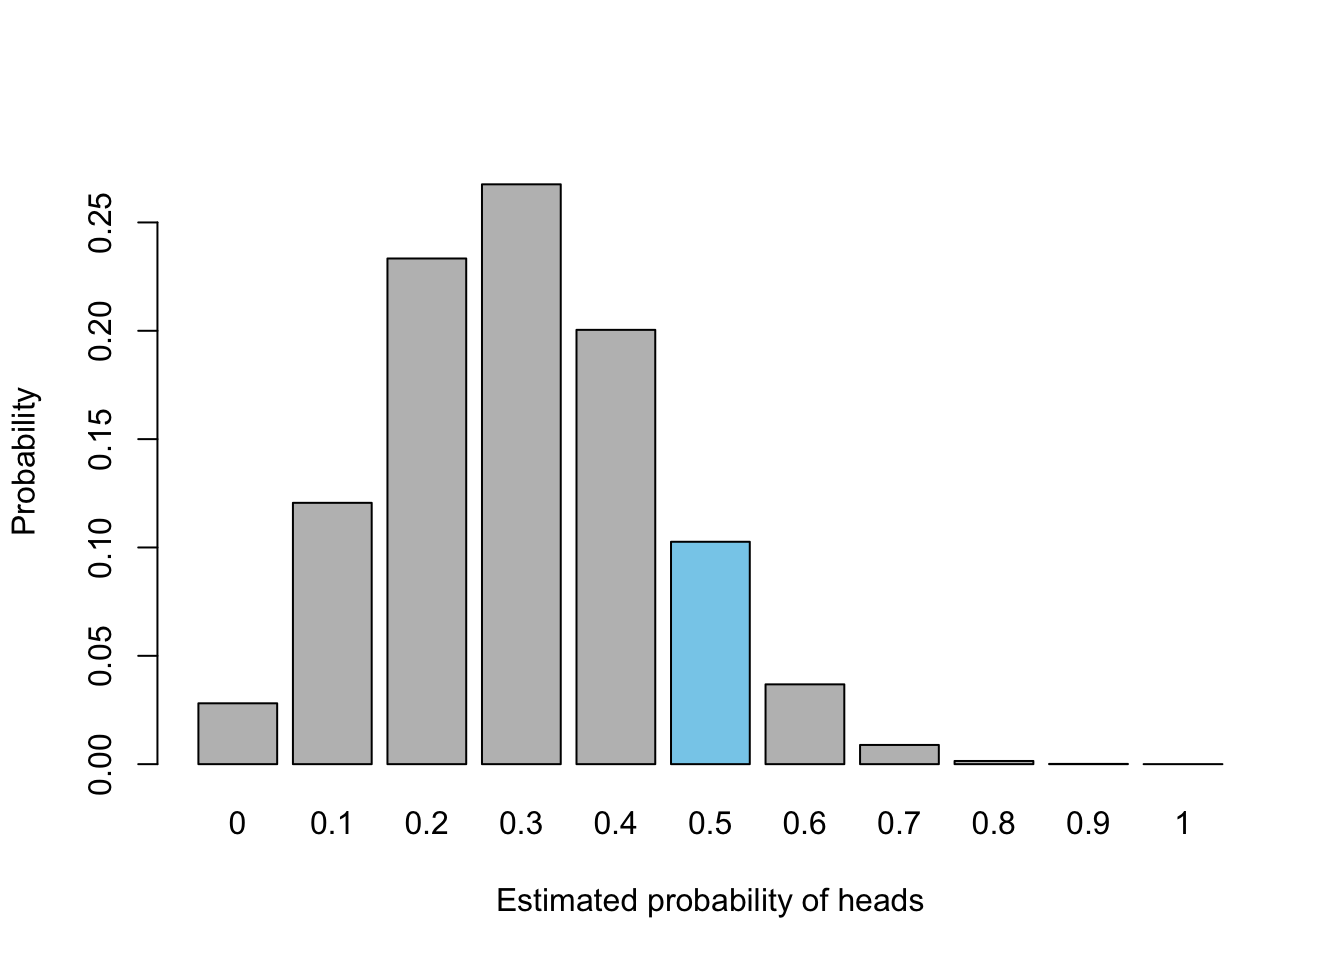
\includegraphics{Research-Design---Statistics_files/figure-latex/c6c7-1.pdf}
\caption{\label{fig:c6c7}Example of a sampling distribution showing biased estimates.}
\end{figure}

Here we can see there's a clear problem in our sampling process. There's variation in the possible estimates just like the first case, but notice that the estimates are more consistently underestimates than overestimates. On average, our estimates are much too low. If the estimates tend to systematically differ from the truth, then the estimates are \textbf{\emph{biased}}. Bias is a consistent discrepancy between the estimates and the true value of the parameter. Estimates may be biased high or biased low (e.g., estimates of 0.20, 0.19, 0.39, 0.32, 0.25, 0.29). When we design a study and sampling process, it is important to use strategies to maximize accuracy (minimize bias). More on that in a bit.

\subsection{Precision}\label{precision}

When we examine the range of possible estimates based on a sampling design, we can examine how much variation we expect to see in the estimates from sample to sample. Consider again the coin flipping sampling process to estimate the probability of heads. When we repeatedly flip a coin 10 times, we know our estimates of the probability of heads will vary because the outcome of each coin flip has an element of chance. Sometimes you end up with 6 heads, other times you get 3 heads. We encounter the sample kind of problem when we sample from any population. Consider again the goal of estimating the proportion of statistics students majoring in biology. If I sample 1000 students, some imprecision is guaranteed because the exact composition of any particular sample of 1000 students is likely to vary just by chance. This chance variation is called \textbf{\emph{sampling error}}, and it leads to some variation in estimates from sample to sample, which we call \textbf{precision}. Precision is a measure of how consistent estimates should be when we repeatedly sample from a population, using the same sampling methodology each time. If the estimates are consistently around the same value, then the estimates are precise. If the estimates vary wildly, then the estimates are imprecise.

From a coarse perspective, we can gauge the precision of an estimate by examining the width of a sampling distribution. Let's visit the coin flipping problem. I've generated two sampling distributions, one where we count the number of heads out of 10 coin flips, and another where we count the number of heads out of 100 coin flips. Each sampling process is repeated 1 million times, and the sampling distributions show the variation in estimates of the probability of heads (Figure \ref{fig:c6c8}. What do you notice that's different between these sampling distributions?

\begin{figure}
\centering
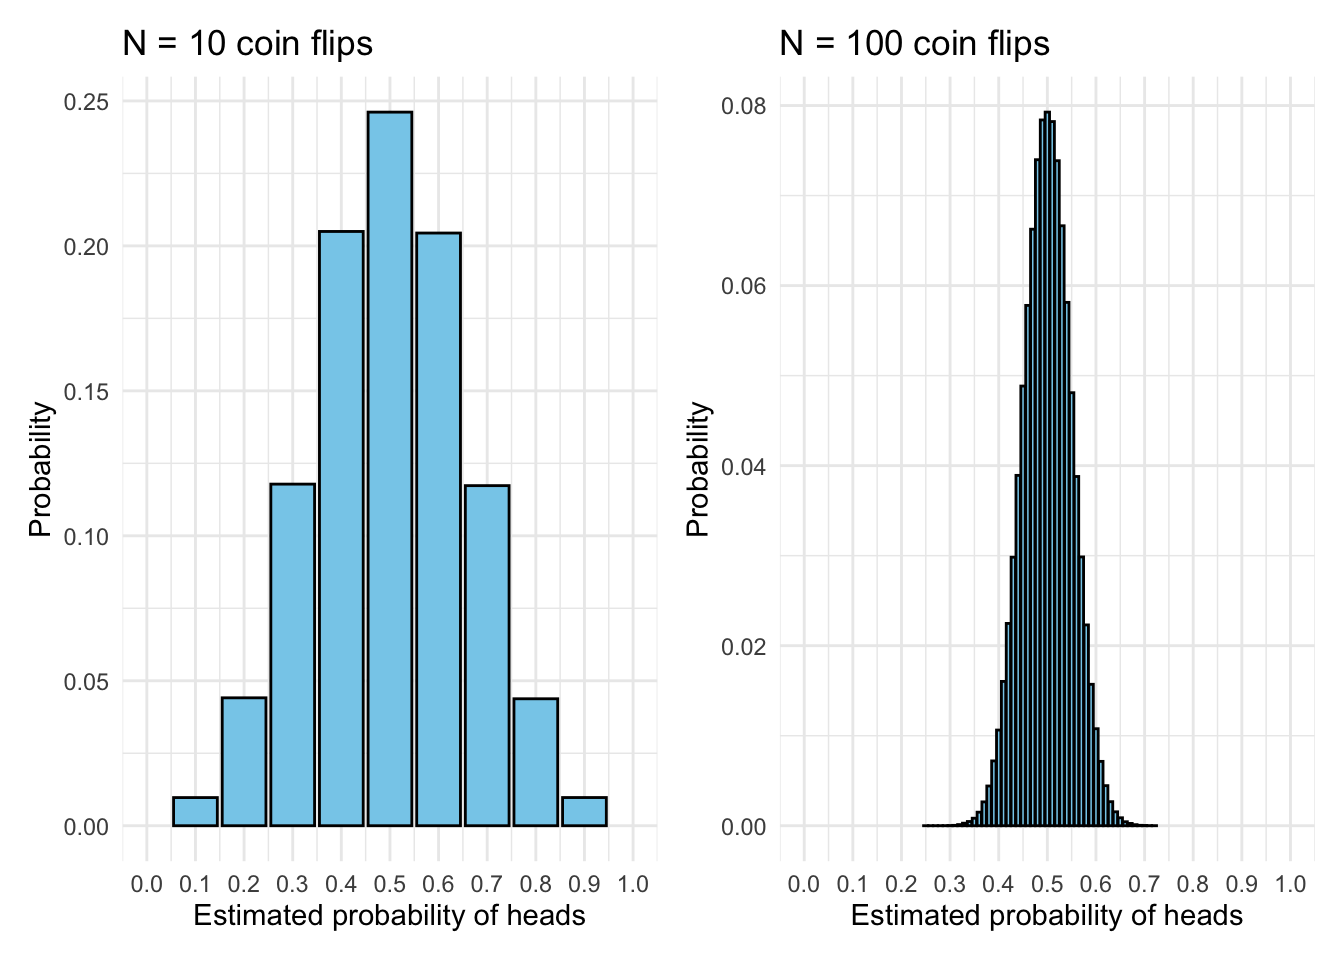
\includegraphics{Research-Design---Statistics_files/figure-latex/c6c8-1.pdf}
\caption{\label{fig:c6c8}Sampling distributions for estimates of the probability of heads based on samples of size 10 (left) vs.~100 (right).}
\end{figure}

These sampling distributions differ in a couple important ways. First, notice that the sampling distribution for N = 10 coin flips is wider than the sampling distribution for N = 100. This is a clear difference in precision between the two sampling approaches. Sampling with N = 10 coin flips leads to less precise estimates of the probability of heads than sampling with N = 100 coin flips. With fewer coin flips, you should expect to see much more variation in the potential estimates. Second, notice that the y-axis scales are different. The most probable outcome under either sampling approach is 0.5 for the probability of heads, but the probability of getting \textbf{exactly} 0.5 as an estimate is much lower when flipping a coin 100 times than when flipping it 10 times. This is simply a consequence of there being many more possible values that you can get for the probability of heads when you flip the coin 100 times. For example, you can get 51/100 = 0.51 for hte probability heads when flipping 100 times, but it's impossible to get 0.51 when you flip a coin just 10 times.

Breaking down the code

Figure \ref{fig:c6c8} shows two sampling distributions for the estimated probability of heads when flipping a coin 10 times vs.~100 times, repeating the sampling process in each case one million times. The simulated data are stored in the objects \texttt{sample10} and \texttt{sample100}. Nothing new there. What's new is that I use the \texttt{dplyr} and \texttt{ggplot2} packages to create a figure of the sampling distributions.

The \texttt{dplyr} package here is used to create a data frame of the possible estimates of the probability of heads \texttt{prob}, the number of times each outcome was observed \texttt{n}, and the computed probability of each outcome \texttt{probabilility}. This is done in two steps. The first step was to initialize the dataframe (\texttt{df10} and \texttt{df100} with the possible values of the probability of heads, \texttt{prob}). Next, the \texttt{dplyr} function was used to computer the observed number of outcomes (\texttt{n}) and probability of each (\texttt{probability}), conveniently adding them to the data frame using the pipe operator, \texttt{\%\textgreater{}\%}. The pipe operator takes the output of one function and passes it as the first argument of the subsequent function, helping to create a sequence of operations that are easier to follow. So in this case, the pipe operator helps create a dataframe of of possible probabilities of heads, observed count of outcomes , and the observed probability of each. The \texttt{mutate} function is used to create a new column in a dataframe based on existing variables, and here is used to quantify the observed probability of each outcome.

The \texttt{ggplot2} package is used to plot the resulting sampling distributions, usingan approach similar to \texttt{dplyr} with a \texttt{+} operator to combine multiple operations to create a graph in one go. The \texttt{ggplot} function initializes the figure with the dataset (\texttt{df10} or \texttt{df100}, assigning \texttt{prob} to the x-axis and \texttt{probability} to the y-axis). The next operation after the \texttt{+} operator is performed by the \texttt{geom\_bar} function, which creates a bar chart. The \texttt{stat\ =\ identity} argument tells \texttt{ggplot2} to make the heights of the bars from the \texttt{probability} column. The following operations are used to adjust the x-axis limits (\texttt{scale\_x\_continuous}) and add labels (\texttt{labs}). The default background theme for \texttt{ggplot2} has gray shading, and I'm not a fan of that, so I add one more operation to add a minimal theme that removes the gray shading.

Note that each figure is assigned a name, \texttt{p1} and \texttt{p2}. The code \texttt{p1\ +\ p2} is executed, which uses the \texttt{patchwork} library to arrange \texttt{ggplot2} figures in a multipanel plot.

I know this is a lot. I'm not a frequent user of \texttt{ggplot2}, but for some types of graphing situations it can be quite handy. Use the exmaples and help documentation to your advantage.

\section{Maximizing accuracy and precision of estimates}\label{maximizing-accuracy-and-precision-of-estimates}

High quality estimates are both accurate and precise. When designing a scientific study, it is critical to design the data collection scheme in a way that will maximize accuracy and precision. Let's go over some attributes of study design that affect accuracy and precision.

\subsection{Random sampling}\label{random-sampling}

The most effective strategy to minimize bias is to take a \textbf{\emph{random sample}} of individuals from the population of interest. A random sample means that every individual in the population has an equal chance of being included in the sample. For our study of sunscreen and skin cancer, the best approach is to identify people in the population of interest, and then randomly sample a subset of those individuals for inclusion in the study. Of course that's easier said than done.

When working with people, it's often difficult to obtain a perfectly random sample, but it's better to be aware of potentially biases in a sample than to ignore them. Consider again the sample of patients to estimate the relationship between sunscreen and skin cancer. Those patient records were simply easy to access, so the individuals in the study were a \textbf{\emph{sample of convenience}}. This is less than ideal because samples of convenience are typically not representative of the broader population of interest. Patients are typically more likely to visit the doctor if they have a problem to begin with, so one concern is that we may be overestimating the prevalence of skin cancer. Conversely, what if the people most likely to visit the doctor also tend to be proactive about their health? Perhaps the people who are more inclined to visit the doctor are more likely to use sunscreen. If the patients most likely to visit the doctor are ones who tend to use sunscreen and tend to visit the doctor because of a symptom, then we might find skin cancer is more prevalent among sunscreen users, an inaccurate conclusion. Samples of convenience often cause bias.

Bias in estimates is similarly caused by \textbf{\emph{volunteer samples}}. The classic case is survey design. Suppose small town is debating about purchasing land to build a park for recreation. The park will include a playground, a splash pad, fields for soccer, baseball, and football, and some tennis courts. The tennis courts and fields will all have lights, allowing people to play in the evenings. The town board wants to see if residents support the idea of building the new park, so they create a survey and mail it to residents. Who's most likely to respond? In this case, volunteer bias would occur if the people most likely to respond are ones who have very strong opinions. For example, residents who are really passionate about having recreation fields may be most likely to respond, causing an overestimate in the proportion of residents who favor creating the park. Conversely, imagine there's a large neighborhood next to the land being considered for purchase, and those residents don't want bright lights on at night in their backyard. Support for the park may be underestimated if the residents in that neighborhood are more inclined to respond to the survey.

\textbf{Important note}: Random sampling is not the same as randomization in an experiment. When we refer to random sampling, we're talking about how individuals are selected from the broader population to participate in a study. Randomization refers to the random assignment of individuals to treatments once they are enrolled in the study.

\subsection{Replication}\label{replication}

The clearest way to maximize precision (i.e., minimize sampling error) is to maximize replication, the number of independent sampling units in a study. The number of indepenent sampling units is also referred to as the \textbf{\emph{sample size}}. Remember that sampling error is the chance variation in estimates due to sampling only a subset of indidivudals from a population. If you could include all individuals from the population in your study, there would be no sampling error. Sampling error decreases as you increase the sample size. We proved this to ourselves with the coin flipping example. There was much more variation in estimates of the probability of heads when flipping a coin 10 times than when flipping a coin 100 times. If you increase the sample size to even greater than 100 coin flips, the estimates will be much more precise.

Note that I defined replication as ``the number of \textbf{independent} sampling units. Independence is really important, because it affects how you count sampling units and ultimately determine the sample size in a study. Replicates are independent if the measurements from one replicate have no influence on the measurements from other replicates. Sometimes individuals in a study are not independent. For example, consider again the survey about building a park. Should the researcher include multiple people from the same household in the survey? They certainly could, but the responses of individuals from the same household are likely correlated. In other words, individuals from the same household may have similar preferences about the park. If you included these individuals in your study and counted them as independent replicates, your estimates will be less precise than you think. Counting individuals as unique replicates when they are not independent is referred to as \textbf{\emph{pseudoreplication}} and can lead to incorrect inferences. More on that later!

\textbf{Important note}: Sample size affects precision, but it does not affect accuracy of estimates. Remember that accuracy is how close, \textbf{on average}, your sample estimates are to the true value of the parameter. There's no inherent effect of sample size on accuracy. In other words, low sample size does not cause bias. Consider the coin tossing example. Estimates of the probability of heads varied quite a bit more when using sample sizes of 10 flips rather than 100 flips. In other words, the estimate are less precise with a sample size of 10. But using 10 flips did not introduce bias (i.e., a consistent underestimation or overestimation of the probability of heads). Both sampling distributions are centered on the true probability of heads, 0.5.

\section{Study design elements specific to experiments}\label{study-design-elements-specific-to-experiments}

Random sampling and high replication are arguably the two most important properties of good samples in that they are principles that apply to virtually any study, experimental or observational. There are some additional elements of study design that can help maximize accuracy and precision that are particularly relevant in experiments. Let's work through a few.

\subsection{Control groups}\label{control-groups}

Control groups are mainly applicable to experiments where researchers randomly assign individuals to different treatments. Suppose a study is being designed to test the effect of a vaccine on the probability of getting Covid. Researchers enroll 100 people in the study and follow them for two years. In the first year, no one gets the vaccine. In the second year, everyone gets the vaccine. The probability of getting Covid was 15\% in the first year and 5\% in the second year, so a 10\% reduction in the year when the vaccine was administered. Was the reduction in the risk of Covid caused by the vaccine? Unfortunately, it's hard to say because the researchers did not include a control group, a group that does not receive the treatment of interest. Maybe Covid was simply more virulent (more likely to infect people) in the first year than the second year, and virulence of covid strains is confounded with treatment. If that were the case, a control group would also show a reduction in the probability of covid from year one to year 2. Control groups help researchers make accurate inferences about causation by providing a baseline for comparison to the experimental treatment.

Control groups are often considered *\textbf{placebos}, which refers to a fake treatment. Good placebos mimic the process of the actual treatment to the greatest extent possible. For example, the control group in the vaccine study would receive a needle injection just like the treatment group with the vaccine, except the placebo would involve injection of salt water. The treatment and placebo injections should be the same amount of liquid and injected in the same place. Keeping treatment and placebo groups as similar as possible helps to isolate the difference between the treatment and control group directly to the treatment effect of interest (i.e., the vaccine).

\textbf{Important note:} Not every experiment has a control group, per se. Imagine you are studying the effect of different doses of a medication for acid reflux: 10 mg, 20 mg, 30 mg once a day. One does not absolutely need a control group to compare the degree of acid reflux among these treatment groups. A control group \textbf{would} be needed if the researchers wanted to test whether the medication reduces the amount of acid reflux relative to untreated individuals.

\subsection{Control of variation}\label{control-of-variation}

Consider again the study of the effect of medication doses on acid reflux. One important element of experimental design is controlling for sources of variation in the response variable other than the treatment. For example, the researchers wouldn't want some participants to take their 10 mg pill with water and other participants to take the pill with soda, as that could introduce variation in reflux independent of the treatment. Statistically, controlling other sources of variation in an experiment will help increase precision of estimates.

\textbf{Important note:} Controlling variation in an experiment is different than creating a control group.

\subsection{Blocking}\label{blocking}

Sometimes it's difficult to control for strong sources of variation in an experiment. For example, in the study on acid reflux, individuals might vary dramatically in their diet, which can introduce a lot of variation in acid reflux independent of the effect of the medication. In a case like this, researchers might use a \textbf{\emph{blocked design}}, which involes stratifying the participants in the study into different groups, or blocks. In the acid reflux case, individuals could be stratified into groups based on diet (e.g., high acidity vs.~low acidity diet). Once the blocks are defined, the researchers would then randomly assign each of the treamtents to individuals in each block. By assigning each treatment to individuals in each block, one can avoid any confounding between the treatments and the factor being blocked.

\subsection{Blinding}\label{blinding}

Blinding is helpful to avoid bias in experiments. It applies to cases when bias can be introduced by either the experimenter or subjects knowing which treatments were applied to individual subjects. For example, a patient who knows they received a vaccine treatment might behave differently than a patient who knows they received a placebo. Maybe the patient who knows they received the vaccine will be more inclined to spend time indoors in crowded spaces when Covid is circulating widely, which may increase their risk of getting covid. To minimize this kind of bias, patients are often blinded to the treatment they receive. Experimenters sometimes need to be blinded too. For the study on acid reflux, suppose a laryngologist is quantifying the degree of reflux in each patient by scoring the amount of redness in the larynx upon examination. If the laryngologist knows a patient received the maximum dose, they may be more skeptical about recording very high values of redness given that the expected effect of the drug is to reduce reflux. To avoid this bias, individuals who make observations of experimental subjects are often blinded from knowing the treatment the subject received.

\chapter{Probability}\label{probability}

One of the central goals of epidemiology is to monitor and understand the prevalence of disease. Basic information on the prevalence of disease is used by public health officials to guide decision-making on interventions. Perhaps there's no better example of this than the Covid-19 pandemic that started in late 2019 and led to dramatic measures intended to reduce the spread of the virus, such as social distancing, mask wearing, travel restrictions, school shutdowns, and quarantine. These interventions place significant limitations on the freedoms that we tend to take for granted, and so the benefits of these measures to the public must outweigh the costs.

In this chapter, we will use a simplified version of monitoring disease prevalence to explore concepts about \emph{probability}. Here's the scenario. Imagine you're the lead epidemiologist in a local community of 10,000 people working with public health officials to make decisions about interventions to minimize the spread of a new viral disease. Based on a cost-benefit analysis, public officials have determined that interventions will be enforced if the prevalence of the disease reaches a 10\% threshold. As the lead epidemiologist, your primary goal is to estimate the prevalence of the disease by testing individuals. For now we will assume the test is fool proof. When someone has the virus, the test is always positive, and when someone doesn't have the virus, the test is always negative.

You don't have the time or resources to test everyone, so you plan to sample individuals from the broader population for testing. You know now that random sampling is necessary to ensure accurate estimates, and although true random sampling in public health is hard to do, we'll assume you can select individuals randomly for the sake of this example.

You also know that when you estimate a quantity of interest, there is inevitably \textbf{uncertainty} about the estimate due to sampling error. This is the ultimate reason why we need rigorous statistical methods. When we sample from populations, we cannot answer questions with certainty. There is some true, but unknown proportion of people in the community infected with the virus. Your estimate will be burdended with \textbf{uncertainty}, and in order to evaluate the quality of your estimate, we have to work towards quantifying uncertainty, and we do that in terms of probability.

\section{Defining probability}\label{defining-probability}

Let's start with some terms. When we test an individual for infection, the test is called a \emph{trial}. A trial is simply any process that produces a probabilistic \emph{outcome}. There are only two possible outcomes of the test: positive or negative. These outcomes are \textbf{mutually exclusive}, meaning that an individual cannot test positive \emph{and} negative for the infection at the same time. The set of all possible mutually exclusive outcomes is called the \emph{sample space}. The sample space is often denoted \(\Omega\) and defined in brackets. For example, the sample space for infection status is \(\Omega\) = \{positive, negative\}.

When examining a probability, we are interested in the probability of a particular \emph{event} that we a define. The event could be as simple as the occurrence of a single outcome, such as an individual testing positive. But events can also be defined as sets of outcomes. For example, consider tossing a six-sided die, where the sample space is \(\Omega\) = \{1,2,3,4,5,6\}. Here we could define the event as rolling an even number, which includes three of the possible outcomes.

Ultimately probability is a parameter with a numerical value between 0 and 1. It is variably abbreviated as \emph{p} or \emph{P}, but the event of interest is usually appended. For example, we can define the probability of the event of interest ``X'' as \(p_{X}\) or \(P(X)\). In our example, we're interested in the probability of infection, which we can denote \(p_{infected}\) or \(P(infected)\). I will use both of these naming conventions at times throughout the book.

The quantitative definition of probability is pretty straightforward. But philosophically, what does probably actually mean? It turns out there are multiple interpretations of probabilities. Let's take a look at the two most common interpretations:

\subsection{Frequentist definition}\label{frequentist-definition}

The \textbf{frequentist} definition of probability is one you are probably already familiar with: probability is the proportion of trials \emph{n} where we observe the event of interest, \(X\):

\[
P(X) = \frac{X}{n}
\]

Let's just assume for now that of the 10,000 people in the community, 500 are infected with the virus. Under the frequentist definition, the probability of the infection (\(I\)) is

\[
P(I) = \frac{I}{n} = \frac{500}{10000}=0.05
\]

The frequentist definition simply looks at the frequency of the event of interest relative to the total number of trials. A probability is a proportion, thus constrained to values between 0 (where the event of interest does not occur) and 1 (where the event of interest is a certainty). Probabilities can also be expressed as percentages. To do this, simply multiply the proportion by 100. Saying the probability of infection is 0.05 is the same as saying 5\% of the population is infected.

Now in practice, how do we know the frequentist probability? As the formula implies, we could go track down all \(n\) individuals in the population and give them our fool proof test for the viral infection. But you know that tracking down every individual in the population is usually not feasible, so we usually need to estimate the probability of interest with a sample of data. For example, imagine you randomly sample \(n = 15\) individuals and find one of the 15 tests are positive. In this case, the estimated probability of infection (\(\hat{p}\)) is

\[
\hat{p}_{infected} = \frac{I}{n} = \frac{1}{15}=0.067
\]

Remember that the carrot symbol simply indicates that our quantity is an estimate based on a sample.

There is a way of logically deriving true frequentist probabilities, but this approach is restricted to only the most simple of examples, such as tossing a coin or rolling a die, where you can count the number of times the event of interest occurs out of the sample space. When we flip a coin, there are two sides, heads and tails. Assuming we have a fair coin and flip, the probability of heads must be 0.5, because heads represents half of the sample space. Similarly, if we roll a four-sided die with the numbers 1, 2, 3, and 4, the probability of seeing a ``four'' must be 0.25, because four represents one out of four possible outcomes.

Why doesn't this logic of deriving frequentist probability mathematically work when applied to our viral test? After all, each individual is infected or not infected. In this limited sample space, infected represents one of two possible outcomes, so isn't the probability of infection 0.5? No! When we derive the probability of heads when flipping a coin, or the probabity of rolling a \emph{4} on a four-sided dice, it is important to note that we made important assumptions. We assumed we have fair coin flips and fair dice, and we assumed coin flips and dice tossing is conducted in a random way. In other words, deriving probabilities mathematically from the sample space inevitably requires assumptions about the external forces that can affect the probability of heads, or the probability of rolling a four. If I do not give the coin a fair toss, for example by just dropping the coin flat with the heads face up, then the probability of heads will very likely \emph{not} be 0.5. There are a multitude of external forces that affect the likelihood of an individual being infected with a virus, such as exposure, immune function, public health measures, and even the prevalence of the infection itself.

\subsection{Bayesian definition}\label{bayesian-definition}

The \textbf{Bayesian} way of thinking about probability is as a strength of belief. What do you believe is the probability of infection? We make these kind of subjective probability assessments all the time. If you look outside and see storm clouds on the horizon, you might be inclined to believe it's more likely than not that it will rain today. When you are deciding which route to take to work, you might notice it's the middle of rush hour and conclude there's a 90\% chance that you'll end up in stop-and-go traffic on the interstate. When watching your favorite college basketball team take on the \#1 ranked team, you might conclude your team has only a 10\% chance of winning.

These subjective beliefs aren't empirically computed by frequencies across multiple trials. Rather, they are subjectively computed in your mind based on your knowledge, experience, and intuitions. If you've never heard of anyone being infected with the viral infection being investigated, you might be inclined to conclude it's more likely than not that the prevalence of the virus is below 10\%. In this case you're assigning a subjective probability statement (\textgreater50\% strength of belief) about the frequentist value of a probability (the proportion of individuals infected being below 10\%).

In \href{https://sites.google.com/site/doingbayesiandataanalysis/}{\emph{Doing Bayesian Data Analysis}}, the author John Kruschke talks about how subjective beliefs about probability can be calibrated by comparing those beliefs with events that have known probabilities. For example, suppose I offer you two choices. You can win \$20 if you flip a coin and the result is heads, or you can win \$20 if your favorite college basketball team beats the \#1 ranked team. If you choose the coin flip, you are implicitly concluding that the probability of your team winning is less than 50\%.

Now, Bayesian probabilities aren't always completely subjective. Indeed, much of Bayesian data analysis that we will encounter in the book involves updating our subjective beliefs about a probability (which we will call a \emph{prior probability}) with frequentist probabilities informed by data that we collect. Stay tuned!

\section{Probability rules}\label{probability-rules}

One can take an entire course on the mathematics and theory of probability, but here our goal is to apply some basic knowledge of probability to science and data analysis. That said, familiarity with some basic rules of probability is necessary to do applied statistics. Let's take a look at those rules \footnote{These basic probability rules apply whether you interpret probability based on frequencies of events or strength of belief.}.

Rule 1: The probability of any event X is non-negative.

\[
P(X) \geq 0
\]

Rule 2: The probability of any possible outcome in the sample space \(\Omega\) is certain (1).

\[
P(\Omega) = 1
\]

This rule implies that the probability of all mutually exclusive outcomes must add to 1.

Rule 3: Addition rule

\[
P(A\ \text{or}\ B) = P(A) + P(B)
\]
If outcomes A and B are mutually exclusive, then the probability of either A or B occurring is the sum of their individual probabilities.

Let's apply the addition rule to an example. Consider a six-sided dice with \(\Omega\) = \{1, 2, 3, 4, 5, 6\}. When the dice is rolled, each outcome is mutually exclusive, so we can apply the addition rule to quantify the probability of one event or another. For example, the probability of rolling a ``1'' or ``2'' is.

\[
P(1\ \text{or}\ 2) = P(1) + P(2) = \frac{1}{6}+\frac{1}{6}=0.333
\]
We can extend this rule beyond two events. For example, the probability of a ``1'', ``2'', or ``3'' is

\[
P(1\ \text{or}\ 2\ \text{or}\ 3) = P(1) + P(2) +P(3) = \frac{1}{6}+\frac{1}{6}+\frac{1}{6}=0.5
\]
The first three probability rules above are known as \textbf{Kolmogorov's Axioms of Probability}, named after the Russian mathematician Andrey Kolmogorov. Rules 1 and 2 together imply that probability is mathematically bounded between 0 and 1: \(0 \leq P(X) \leq 1\), and Rule 3 allows us to quantiy the probability of one or more mutually exclusive events. From these three rules, we can derive a fourth rule:

Rule 4: Not rule

\[
P(\text{not}\ A) = 1 - P(A)
\]
The probability of an event not occurring is one minus the probability that it occurs.

For example, when rolling a six-sided dice, the probability of not rolling a ``5'' can be quantified as

\[
P(\text{not}\ 5) = 1 - P(5) =1-\frac{1}{6}=0.833
\]
\#\# Joint events

The first four rules apply to events in isolation, but often we are interested in the joint probability of multiple events occurring at the same time. For this situation let's consider again the goal of estimating the prevalence of a viral infection. The epidemiologist does not know the true prevalence, but let's assume it's 5\%. The epidemiologist randomly samples two people from the population and surprisingly finds that both are infected! What was the probability of two randomly-selected individuals being infected when the prevalence of the infection is 5\%? Here we are interested in a \textbf{joint probability}, namely the probability of the first \emph{and} second individuals being infected.

\subsection{Joint events under independence}\label{joint-events-under-independence}

In cases where the joint events are \textbf{independent}, we can apply the following rule to quantify the joint probability:

Rule 5: Multiplication rule

\[
P(A\ \text{and}\ B) = P(A)P(B)
\]

When events A and B are independent, the probability of A and B is the multiplication of the probabilities of A and B individually.

For events to be independent, one event must have no impact at all on the probability of another event. In the context of testing, this would mean that the infection status of individual A must have no impact on the infection status of individual B. The infection status of both people must be completely unrelated. If that's the case, then we can quantify the probability of individuals A and B both being infected as

\[
P(infected\ and\ infected) = 0.05*0.05=0.0025
\]

When the prevalence of the infection is 5\%, the probability that two randomly-selected individuals will both be infected is only 0.25\%. A rare event indeed!

Consider another example. According to the \href{https://www.pewresearch.org/short-reads/2023/08/15/32-of-americans-have-a-tattoo-including-22-who-have-more-than-one}{Pew Research Center}, approximately 32\% of Americans have a tattoo. Let's assume that's the case in the community of interest. If one individual is selected at random, what is the probability the individual is infected \emph{and} has a tattoo. Assuming these are independent events, the probability can be quantified as

\[
P(infected\ \text{and}\ tattoo) = 0.05*0.32=0.016
\]

\subsection{Joint events under non-independence (conditional probability)}\label{joint-events-under-non-independence-conditional-probability}

Are we making good assumptions? Is the probability of a viral infection really independent of having a tattoo? I doubt there's a direct causal effect of having a tattoo on infection status (or vice-versa), but might there be differences in behavior between people with and without tattoos that could affect infection status? Some pyschological studies have shown that people with tattoos tend to score higher on extraversion than people without tattoos (e.g., \href{https://journals.sagepub.com/doi/abs/10.2466/09.07.21.PR0.111.4.97-106?casa_token=GG6UgmonrdAAAAAA:REJHZeVgnjOn2KVpShnrxHf-9M5QSt-TMPkMgliduw_ZaGClESfJkRM3hYkIlXz5xaWDgCp6B_Nr}{Swami et al.~2012}. If people with tattoos are more open or social and therefore around other more than individuals without tattoos, perhaps people with tattoos will be exposed to a virus more than people without tattoos.

Or what about independence when we sample two individuals for testing? Are the results of those tests really independent? If the individuals were truly selected at random, I suspect the independence assumption holds in that case. But we can imagine cases where the outcomes are not independent. For example, what if the two individuals are in the same household, with largely the same set of exposures (including each other)? That's a fairly clear example where we should not expect the outcomes to be independent.

This is getting interesting! Indeed, non-independence of joint probabilities is, from a very mathematical perspective, at the heart of scientific research questions, particular questions about explanation. Does social behavior affect infection status? Such a question can be addressed quantitatively by examining joint probabilities under assumptions of independence vs.~dependency between the events.

To analyze joint probabilities of multiple events when those events are not independent, we need to define \textbf{conditional probability}. A conditional probability can be defined as the probability of event A given that know event B is true. Let's formalize another rule:

Rule 6: Conditional probability

\[
P(A|B) = \frac{P(A\ \text{and}\ B)}{P(B)}
\]

The vertical bar (\textbar) means ``given'', so \(P(A|B)\) reads ``the probability of A given B''. For example, suppose we know someone has a tattoo. Might that give us some information on whether or not they are infected? Consider Table \ref{tab:c7t1}, which shows simulated data for the number of individuals out of 10,000 with each combination of outcome for infection and tattoo status.

\begin{table}
\centering
\caption{\label{tab:c7t1}<span style='color:black; font-weight:bold;'>Counts of Infection Status vs. Tattoos (N = 10,000)</span>}
\centering
\begin{tabular}[t]{l|r|r|r}
\hline
Status & Tattoo Count & No Tattoo Count & Total Count\\
\hline
Infected & 250 & 250 & 500\\
\hline
Not Infected & 2950 & 6550 & 9500\\
\hline
Total & 3200 & 6800 & 10000\\
\hline
\end{tabular}
\end{table}

Let me point out a couple important things about Table \ref{tab:c7t1}. First, notice that we can see the overall probability of infection is 5\% as we previously assumed. There are 500 total people infected out of 10000. We can also see the overall probability of having a tattoo is 32\%, as 3200 out of 10,000 people have tattoos. These probabilities are called \textbf{marginal probabilities} because we are marginalizing the probabilities across levels of a different variable. In other words, to get the total probability of infection, we have to use the data on infection of both tattooed and non-tattooed people, and to get the probability of tattoo, we have to use the data on tattos for both infected and non-infected people.

Second, from these data we can compute the joint probabilities of each combination of events:

\begin{Shaded}
\begin{Highlighting}[]
\DecValTok{250}\SpecialCharTok{/}\DecValTok{10000} \CommentTok{\#Infected and Tattoo}
\end{Highlighting}
\end{Shaded}

\begin{verbatim}
## [1] 0.025
\end{verbatim}

\begin{Shaded}
\begin{Highlighting}[]
\DecValTok{2950}\SpecialCharTok{/}\DecValTok{10000} \CommentTok{\#Not infected and Tattoo}
\end{Highlighting}
\end{Shaded}

\begin{verbatim}
## [1] 0.295
\end{verbatim}

\begin{Shaded}
\begin{Highlighting}[]
\DecValTok{250}\SpecialCharTok{/}\DecValTok{10000} \CommentTok{\#Infected and No tattoo}
\end{Highlighting}
\end{Shaded}

\begin{verbatim}
## [1] 0.025
\end{verbatim}

\begin{Shaded}
\begin{Highlighting}[]
\DecValTok{6550}\SpecialCharTok{/}\DecValTok{10000} \CommentTok{\#Not infected and No tattoo}
\end{Highlighting}
\end{Shaded}

\begin{verbatim}
## [1] 0.655
\end{verbatim}

The joint probabilities quantify the proportion of individuals in the total population who meet the definition of both events. Out of all the people in the population, the probability of being infected \emph{and} having a tattoo is \(250/10000 = 0.025\). Note that these four combinations consist of the entire sample space for the joint probability of infection status and tattoo status, so these joint probabilities should sum to 1.

OK, now let's get back to the question of conditional probability. Are the events infection status and tattoo status independent? If they are independent events, then the probability of infection shouldn't depend at all on tattoo status. In other words, the prevalence of the infection be the same for each level of tattoo status. Let's see if that's the case, here applying our rule to quantify conditional probabilities:

\[
P(infected|tattoo) = \frac{P(infected\ \text{and}\ tattoo)}{P(tattoo)}=\frac{250}{250+2950}=0.078
\]

\[
P(infected|no\ tattoo) = \frac{P(infected\ and\ no\ tattoo)}{P(tattoo)}=\frac{250}{250+6550}=0.038
\]
Here we clearly see that the probability of infection is 4\% greater for those with tattoos than those without tattoos. In other words, infection status is \emph{not} independent of tattoo status!

How do we compute joint probabilities when events are not independent? There's a rule for that!

Rule 7: General multiplication rule

\[
P(A\ \text{and}\ B) = P(A|B)P(B)
\]

This general multiplication rule is derived from Rule 6 on conditional probability by simply isolating \(P(A\ and\ B)\). As an example, if I told you the overall proportion of those with tattoos was 32\% and the probability of infection among those with tattoos was 7.8\%, you can quantify the overall probability of those with infections and tattoos as

\[
P(infection\ and\ tattoo) = P(infection|tattoo)P(tattoo)=0.078*0.32=0.025
\]

Note that we can show infection status and tattoo status are not independent by testing the simple multiplication rule (Rule 5). The simple multiplication rule says that the joint probability of independent events is the multiplication of their individual probabilities. Thus, if infection status and tattoo status are independent, the proportion of people who are infected and have a tattoo should be \(0.05*0.32=0.016\). But that's not the case! The table above shows that 250 people out of 10,000 have tattoos and are infected. Our simple multiplication rule doesn't work because it assumes independence, and tattoo status and infection status are not independent in this example.

\subsection{One thing or another (general addition rule)}\label{one-thing-or-another-general-addition-rule}

Let's revisit the situation when we want to know the probability of one event \emph{or} another event. When the events are mutually exclusive, the addition rule tells us to simply add the probabilities of each event. What if the events are not mutually exclusive? For example, what if I randomly select and individual and want to know if that person is infected \emph{or} has a tattoo. If we apply the simple addition rule, we would conclude the probability of infection or tattoo is \(0.05 + 0.32 = 0.37\), but that's not correct. Why not? The problem is that some of the infected people have tattoos! If you just add the overall probability of infection and tattoo, you are double counting those people. To quantify the probability of event A or B when A and B are not mutually exclusive, we need to apply the \textbf{general addition rule}:

Rule 8: General addition rule

\[
P(A\ \text{or}\ B) = P(A) + P(B) - P(A\ \text{and}\ B)
\]

Let's apply this to the infection and tattoo example:

\[
P(infection\ \text{or}\ tattoo) = P(infection) + P(tattoo) - P(infection\ \text{and}\ tattoo)=0.05+0.32-0.025=0.345
\]

Having fun yet?

\subsection{Quantifying marginal probabilities}\label{quantifying-marginal-probabilities}

When working with joint events, sometimes we want to work backwards from disaggregated probabilities to aggregated, or marginal probabilities. For example, suppose you knew the probability of infection separately for individuals who have tattoos and those who don't have tattoos. In probabilistic terms, we know \(P(infection|tattoo) = 0.078\) and \(P(infection|no\ tattoo) = 0.038\). What's the overall prevalence of infection? You might be tempted to compute the simple average of 0.078 and 0.038, but the mean (0.058) is not correct. Why not? The mean does not weight the conditions of tattoo status appropriately. We know 32\% of the population has a tattoo, whereas 68\% of the population does not have a tattoo. We need to account for the fact that more of the population does not have tattoos. The mean applies equal weight to both conditions, effectively assuming that half the population has a tattoo.

To quantify the marginal probability of infection (i.e., marginalizing the probability of infection over the levels of tattoo status), we to basically quantify a weighted mean. This is the \emph{law of total probability}:

Rule 9: Law of total probability

\[
P(A) = \sum_{i=1}^n P(A|B_i)P(B_i),
\]

where \(A\) is event A and \(B_i\) is condition \emph{i} of event \(B\).

Here we see the total (marginal) probability of event A is the weighted average of the probability of A across conditions of event B. Now let's apply this rule to quantify the probability of infection across conditions of tattoo status:

\[
P(infected) = P(infected|tattoo)P(tattoo) + P(infected|no\ tattoo)P(no\ tattoo)
\]

\[
P(infected) =0.078*0.32+0.038*0.68=0.05
\]

\section{Sampling and probability distributions}\label{sampling-and-probability-distributions}

Ok, that was a fair amount of pure probability theory. But this isn't a probability book, or a theory book. This is a book about applied research design and statistics. In this section we begin to apply basic probability theory to practical questions about the ultimate goal of statistics: estimating unknown quantities by sampling.

Let's get back to being the lead epidemiologist. Suppose that instead of randomly testing individuals from the entire community, you are focused on one household. This household has four people, two parents and two kids. Each person in the household can be infected or not infected, and you want to figure out \emph{how many people in the household are infected}. With four people in the household and the sample space being infected or not infected, there are five possible outcomes for the number of infected people in the household, ranging from no one being infected to all four family members being infected.

Sadly you only have two test kits available, so you can't test the whole family. You're going to test two people, and to make matters more simple from a probability perspective, you're going to test the family members \textbf{with replacement}. What that means is you are going to randomly conduct two tests, but each person is available to be selected for both tests. This is analogous to randomly selecting multiple playing cards from a deck, but each time replacing the card you chose before you select a new one.

Suppose you go ahead and randomly conduct two tests and find that one of the two tests was positive, and one of the two tests was negative. In probability terms, we know there was \(X = 1\) positive test out of \(n = 2\) trials. What insight do these data provide into the infection status of the entire family?

The way we're going to interrogate this issue is by quantifying the probability of the data we observed under each of the five possibilities for the proportion of the family infected. As an example, let's assume that only one of the family members is truly infected. In other words, \(p_{infected} = 0.25\). If only one of the four family members is infected, how likely were we to see one positive out of two tests? To answer that question, let's look at all the possible outcomes when we conduct two tests, given that only one member is infected. Figure \ref{fig:c7f1} shows these possibilities in the format of a branching tree.

\begin{figure}

{\centering 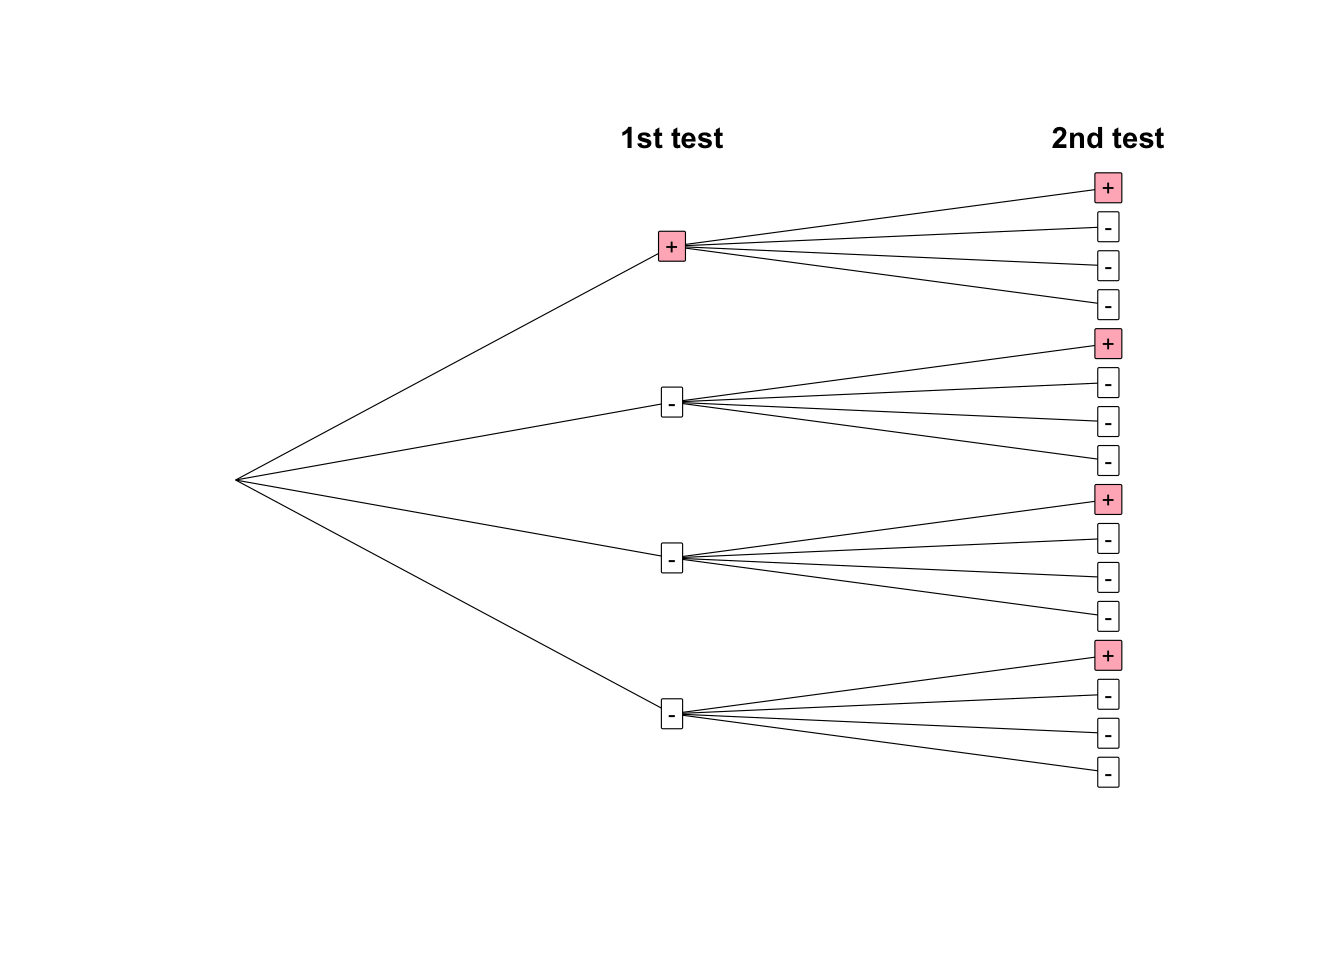
\includegraphics{Research-Design---Statistics_files/figure-latex/c7f1-1} 

}

\caption{Probability tree showing the possible outcomes of testing when one of four people in the household are infected. Pink boxes with + indicate a positive test, and white boxes with - indicate a negative test.}\label{fig:c7f1}
\end{figure}

The boxes in each branch of the tree represents the four family members. Only one of the four members is infected in this scenario, so for the 1st test, we see there's three more ways to see a negative test than a positive test. In other words, when we randomly select an individual for the first test, there's a 25\% chance of a positive test and a 75\% chance of a negative test when one of four individuals is infected. We then repeat that process for the 2nd test. Because we're sampling with replacement, the possibilities on the 2nd test are the same as the 1st test.

We can then see that when one of four family members is truly infected, there are 16 distinct outcomes when we conduct two tests. How many of those outcomes are consistent with the data we observed, that being one positive test and one negative test? There are six possible ways to get one positive test and one negative test. Those outcomes are highlighted in Figure \ref{fig:c7f2}.

\begin{figure}

{\centering 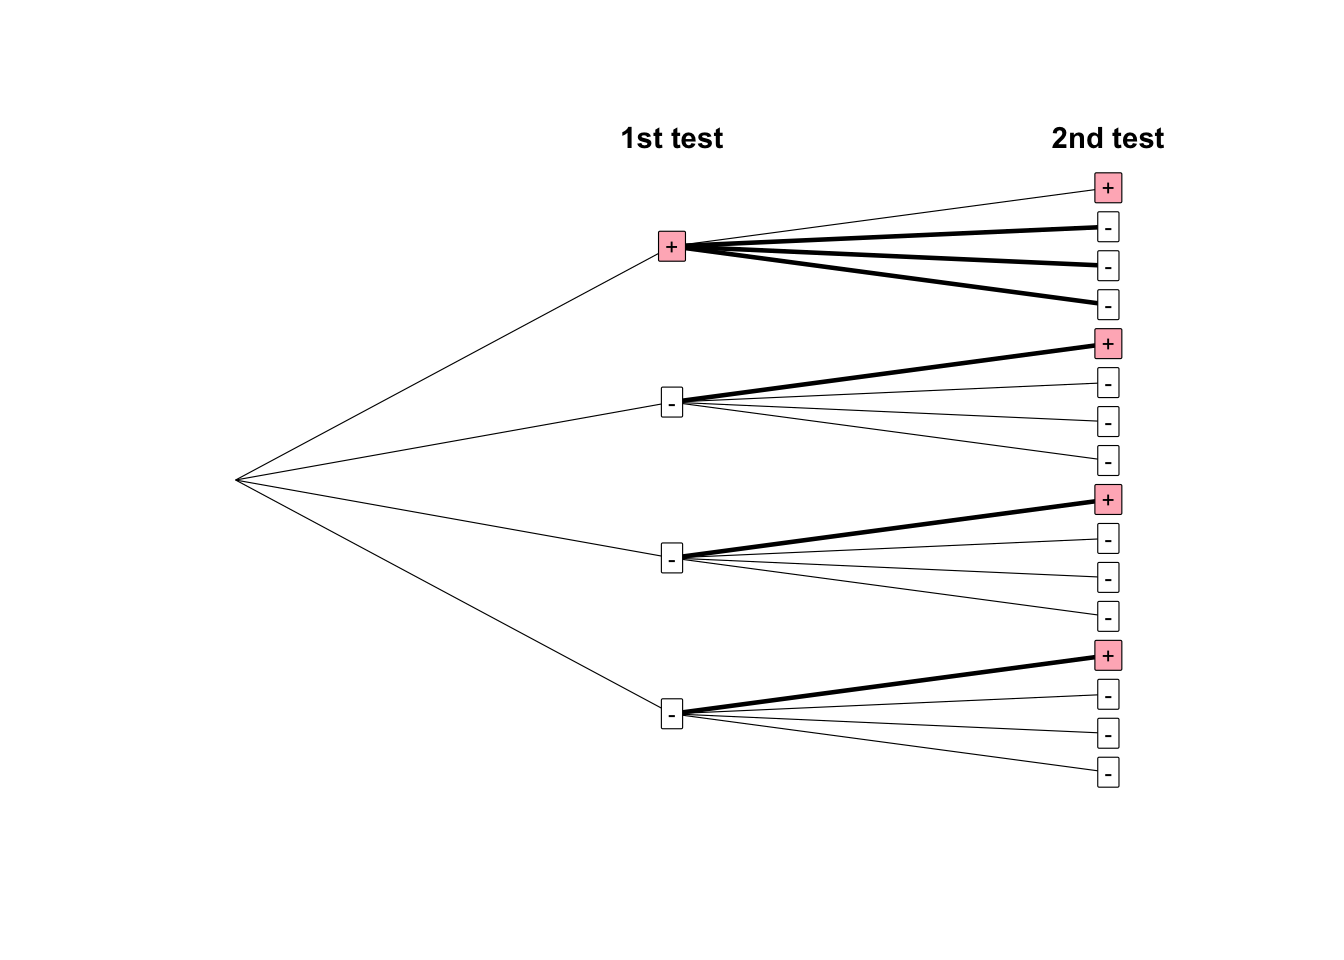
\includegraphics{Research-Design---Statistics_files/figure-latex/c7f2-1} 

}

\caption{Probability tree showing the possible outcomes of testing when one of four people in the household are infected, highlighting outcomes consistent with the observed data.}\label{fig:c7f2}
\end{figure}

Probability trees like this are really handy for looking at all the possible outcomes of joint events, but we can apply our probability rules to compute the probability of one positive out of two tests when the probability of infection is 0.25. You might be tempted to apply the multiplication rule, because we want to know the probability of a positive test \emph{and} a negative test. Applying that rule, we find \(P(+\ \text{and}\ -) = P(+)P(-) = 0.25*0.75=0.1875\). Why isn't this correct? The problem is not independence. We can reasonably assume the test results are independent if we are randomly picking one of the four people in the house for each test. The problem is that there are multiple ways of observing exactly one positive test and one negative test! You can see this in the probability tree. It could be that the first test is positive and the second test is negative (``+-''), which can happen in three ways, or it could be that the first test is negative and the second test is positive (``-+''), which can also happen in three ways. We can separately quantify \(P(+\ \text{and}\ -)\) and \(P(-\ \text{and}\ +)\), and then apply our addition rule because these outcomes are mutually exclusive.

\[
P(\text{One +}\ \text{and}\ \text{One}\ - ) = P(+)P(-) + P(-)P(+)\\
P(\text{One +}\ \text{and}\ \text{One}\ - ) = 0.25*0.75 + 0.75*0.25=0.375
\]
\#\#\# Discrete random variables

At this point I want to formalize some important concepts from our example of conducting two tests in a family of four. What we've just shown is that \textbf{the process of sampling from a population is probabilistic}. When one of four people is infected and we take a sample of \(n = 2\) tests, the outcome that we observe has an element of chance. The outcome \(X\) positive tests is called a \textbf{random variable}, where the term \emph{random} implies an element of chance in terms of how we observe the variable. When we conduct \(n=2\) tests, we can observe one of three mutually exclusive outcomes: X = 0 positives, X = 1 positive, or X = 2 positives. Some of these outcomes are more likely than others, just like getting 5 heads when you flip a coin 10 times is more likely than getting one heads. But there's an element of chance, which is ultimately what creates much of the uncertainty we face when we estimate a quantity.

Every random variable can be characterized by a \textbf{probability distribution}, which is simply the probability of observing each mutually exclusive outcome. Mathematically, we can define the probability that a random variable \(X\) takes on each possible value \(x\) (\(P(X = x)\)). For the random variable \(X\) = \emph{number of positives out of two tests}, the probability distribution consists of \(P(X = 0)\), \(P(X = 1)\), \(P(X = 2)\). We can quantify these probabilities in different ways. First, we could simply enumerate all of the possibilities in the sample space and count up the outcomes. This has basically been done in the probability tree above. Just count the number of ways each value of the random variable can happen, and divide by the total number of possible outcomes:

\begin{Shaded}
\begin{Highlighting}[]
\CommentTok{\#P(X = 0 positives): 9 ways}
\DecValTok{9}\SpecialCharTok{/}\DecValTok{16}
\end{Highlighting}
\end{Shaded}

\begin{verbatim}
## [1] 0.5625
\end{verbatim}

\begin{Shaded}
\begin{Highlighting}[]
\CommentTok{\#P(X = 1 positives): 6 ways}
\DecValTok{6}\SpecialCharTok{/}\DecValTok{16}
\end{Highlighting}
\end{Shaded}

\begin{verbatim}
## [1] 0.375
\end{verbatim}

\begin{Shaded}
\begin{Highlighting}[]
\CommentTok{\#P(X = 2 positives): 1 way}
\DecValTok{1}\SpecialCharTok{/}\DecValTok{16}
\end{Highlighting}
\end{Shaded}

\begin{verbatim}
## [1] 0.0625
\end{verbatim}

Second, we could apply our probability rules:

\begin{Shaded}
\begin{Highlighting}[]
\CommentTok{\#P(X = 0 positives) = P(negative and negative)}
\NormalTok{(}\FloatTok{0.75}\SpecialCharTok{*}\FloatTok{0.75}\NormalTok{)}
\end{Highlighting}
\end{Shaded}

\begin{verbatim}
## [1] 0.5625
\end{verbatim}

\begin{Shaded}
\begin{Highlighting}[]
\CommentTok{\#P(X = 1 positives) = P(positive and negative)}
\NormalTok{(}\FloatTok{0.75}\SpecialCharTok{*}\FloatTok{0.25}\NormalTok{) }\SpecialCharTok{+}\NormalTok{ (}\FloatTok{0.25}\SpecialCharTok{*}\FloatTok{0.75}\NormalTok{) }\CommentTok{\#2 ways this can happen}
\end{Highlighting}
\end{Shaded}

\begin{verbatim}
## [1] 0.375
\end{verbatim}

\begin{Shaded}
\begin{Highlighting}[]
\CommentTok{\#P(X = 2 positives) = P(positive and positive)}
\NormalTok{(}\FloatTok{0.25}\SpecialCharTok{*}\FloatTok{0.25}\NormalTok{) }
\end{Highlighting}
\end{Shaded}

\begin{verbatim}
## [1] 0.0625
\end{verbatim}

Third, we could use R to simulate the process of conducting two tests many, many times, record the number of positives each time, and then quantify the probability of each outcome across all the simulations.

\begin{Shaded}
\begin{Highlighting}[]
\FunctionTok{set.seed}\NormalTok{(}\DecValTok{123}\NormalTok{)}

\CommentTok{\#create a vector representing 25\% infected in a family of 4}
\NormalTok{infections }\OtherTok{\textless{}{-}} \FunctionTok{c}\NormalTok{(}\DecValTok{1}\NormalTok{, }\FunctionTok{rep}\NormalTok{(}\DecValTok{0}\NormalTok{, }\DecValTok{3}\NormalTok{))}

\CommentTok{\#create an empty vector to store the number of positives across 1 million sims}
\NormalTok{x }\OtherTok{\textless{}{-}} \FunctionTok{rep}\NormalTok{(}\ConstantTok{NA}\NormalTok{, }\DecValTok{1000000}\NormalTok{)}

\CommentTok{\#simulate 2 tests 1 million times \& record \# positives each time}
\ControlFlowTok{for}\NormalTok{(i }\ControlFlowTok{in} \DecValTok{1}\SpecialCharTok{:}\FunctionTok{length}\NormalTok{(x)) \{}
\NormalTok{  x.trial }\OtherTok{\textless{}{-}} \FunctionTok{sample}\NormalTok{(infections, }\DecValTok{2}\NormalTok{, }\AttributeTok{replace=}\ConstantTok{TRUE}\NormalTok{)}
\NormalTok{  x[i] }\OtherTok{\textless{}{-}} \FunctionTok{sum}\NormalTok{(x.trial)}
\NormalTok{\}}

\CommentTok{\#quantify the probability of each outcome}
\FunctionTok{prop.table}\NormalTok{(}\FunctionTok{table}\NormalTok{(x))}
\end{Highlighting}
\end{Shaded}

\begin{verbatim}
## x
##        0        1        2 
## 0.561914 0.375773 0.062313
\end{verbatim}

Let's walk through this code. First, the vector \texttt{infections} is created to represent the infection status of each member of the family, where a \texttt{1} represents an infected individual, and \texttt{0} represents uninfected individuals. Next, a vector \texttt{x} is created to store the results of the simulations. The vector is initiated with all NA values. Third, the simulation is conducted with a \texttt{for} loop. A \texttt{for} loop is a programming approach to execute a block of code repeatedly for a specified number of times. The total number of simulations should be the length of the \texttt{x} vector for the output, which is 1 million. The loop executes the code each each time, where \texttt{i} is the particular iteration (1 to 1,000,000). In each iteration, the \texttt{sample} function is used to randomly sample two observations from infections with replacement (\texttt{replace=TRUE}), which returns a vector \texttt{x.trial} of the observations (\{0,0\}, \{0,1\}, \{1,0\}, or \{1,1\}). We then sum the values of \texttt{x.trial}, which represents the number of positives, and store that value in \texttt{x}. Finally, the \texttt{prop.table} and \texttt{table} functions are used to compute the probability of each outcome. Lo and behold, we see largely the same quantities of probability for each value of \texttt{x} as we saw before. These aren't exact probabilities because they are based on a finite number of simulations (another great illustration of how we can't escape uncertainty when sampling).

The probabilities for each possible of outcome, no matter how we quantify them, form a probability distribution. This particular example is a \textbf{discrete probability distribution} because the sample space is composed of discrete, mutually exclusive outcomes where we can quantify the probability of each as we have done. Figure \ref{fig:c7f3} shows the probability distribution.

\begin{figure}

{\centering 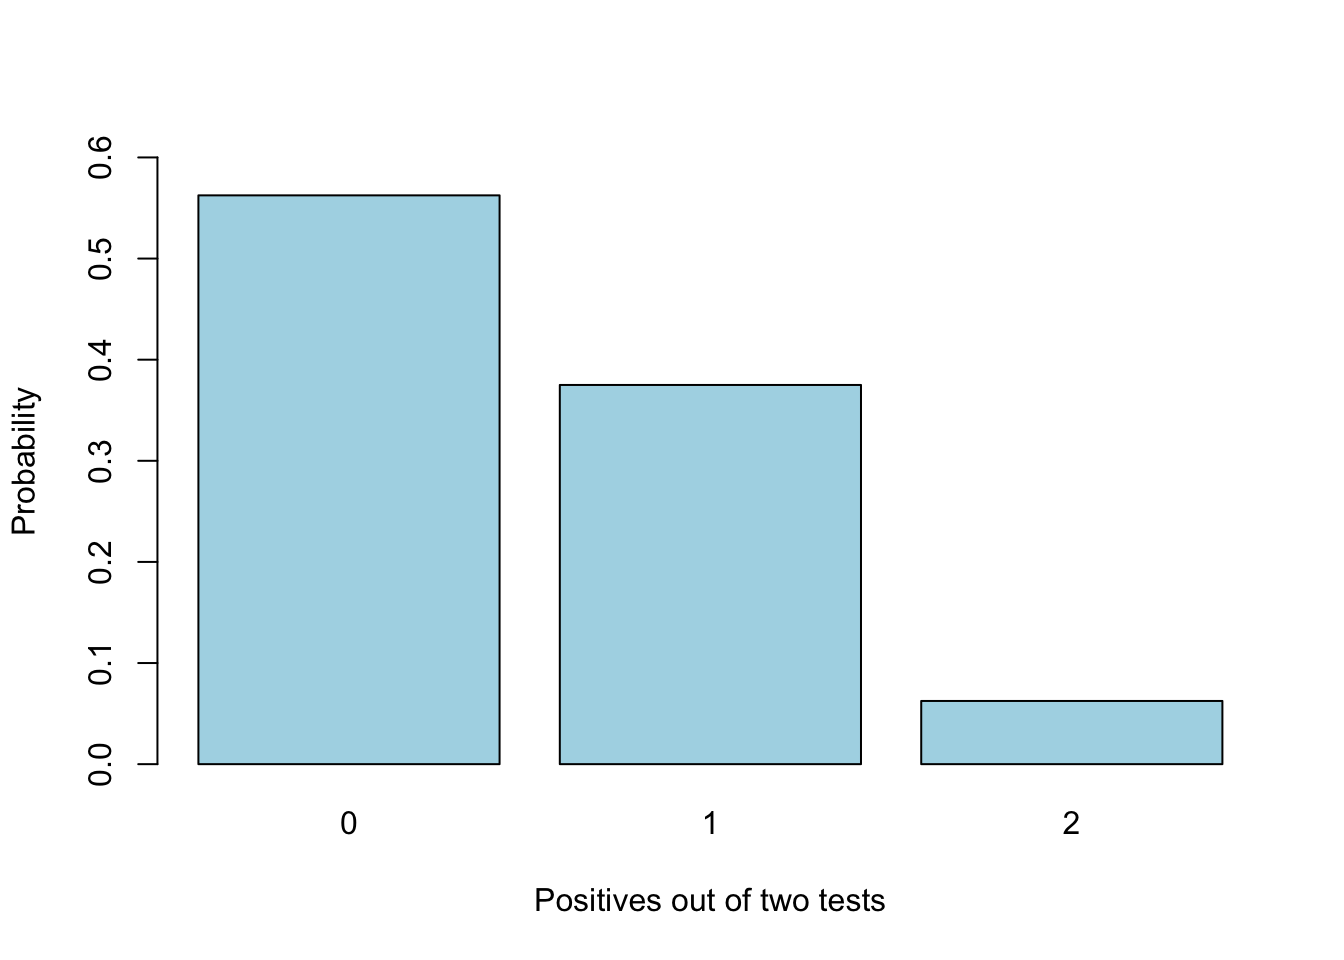
\includegraphics{Research-Design---Statistics_files/figure-latex/c7f3-1} 

}

\caption{Discrete probability distribution of the number of positive tests out of two trials.}\label{fig:c7f3}
\end{figure}

The probability of discrete outcomes is referred to as \textbf{probability mass}, but as Figure \ref{fig:c7f3} shows, the y-axis of discrete probability distributions will often just be labeled ``probability''.

\subsubsection{Binomial distribution}\label{binomial-distribution}

It was pretty straightforward to quantify the probability distribution for the number of positives out of only two tests. The sample space is so small that we could easily quantify those probabilities by applying our probability rules. But what if we randomly conduct 10 tests, or 100 tests, or 1000 tests from the broader community of 10,000? Manually enumerating the probability distribution for each possible number of positives would take considerable time! Fortunately we don't have to do that.

The random variable that we defined - the number of positives \emph{X} out of \emph{n} trials - is actually an example of a variable that follows a known mathematical function called the \textbf{binomial distribution}. A binomial distribution is a probability distribution for a binary variable where the outcome of that binary variable is examined across \emph{n} trials {[}\^{}ch07-2{]}. The sample space of each trial must be binary, for example heads and tails when flipping a coin, even or odd when rolling a die, and positive or negative when testing for a viral infection. The outcome being recorded is often generically referred to as a \textbf{success}. The \emph{n} trials must be independent and have the same probability of success, \emph{p}, which is the only parameter for the binomial distribution (e.g., probability of positive test). If those assumptions are met, the probability of \emph{x} successes out of \emph{n} trials can be computed with the binomial formula:

\[
P(X = x) = \binom{n}{x} p^x (1 - p)^{n - x}
\]
{[}\^{}ch07-2{]}: Each individual trial of a binomial process is called a \textbf{Bernoulli trial}. The \(binom{n}{x}\) part of the formula reads ``n choose x'' and represents the number of ways \emph{x} successes can occur out of \emph{n} trials without regard to order (i.e., \textbf{combinations}). For example, we've already seen that 1 positive test can occur in two ways based on 2 trials. The number of combinations can be quantified as

\[
\binom{n}{x} = \frac{n!}{x!(n-x)!}
\]
Suppose I randomly sample 10 people from the community of 10,000 where the prevlaence of infection is 0.05. What's the probability of observing exactly two infections? Just apply the binomial formula:

\[
P(X = 2) = \binom{10}{2} 0.05^2 (1 - 0.05)^{10 - 2}=0.075
\]
I'm not going to go into details here, but if you work through this formula, you'll see that all it's doing is applying the multiplication rule for independent events and the addition rule for mutually exclusive outcomes. And fortunately for us, we don't have to do these calculations by hand because R has a built-in function to compute the binomial probability: \texttt{dbinom}. For example, we can use the function to quantify the probability of 2 infections out of 10 trials:

\begin{Shaded}
\begin{Highlighting}[]
\FunctionTok{dbinom}\NormalTok{(}\AttributeTok{x =} \DecValTok{2}\NormalTok{, }\AttributeTok{size =} \DecValTok{10}\NormalTok{, }\AttributeTok{prob =} \FloatTok{0.05}\NormalTok{)}
\end{Highlighting}
\end{Shaded}

\begin{verbatim}
## [1] 0.0746348
\end{verbatim}

We can apply the \texttt{dbinom} formula to efficiently compute the binomial probability of all possible values of X positive tests out of 10 trials, when the probability of infection is 0.05, and then display the probability distribution in a graph (Figure \ref{fig:c7f4}):

\begin{figure}

{\centering 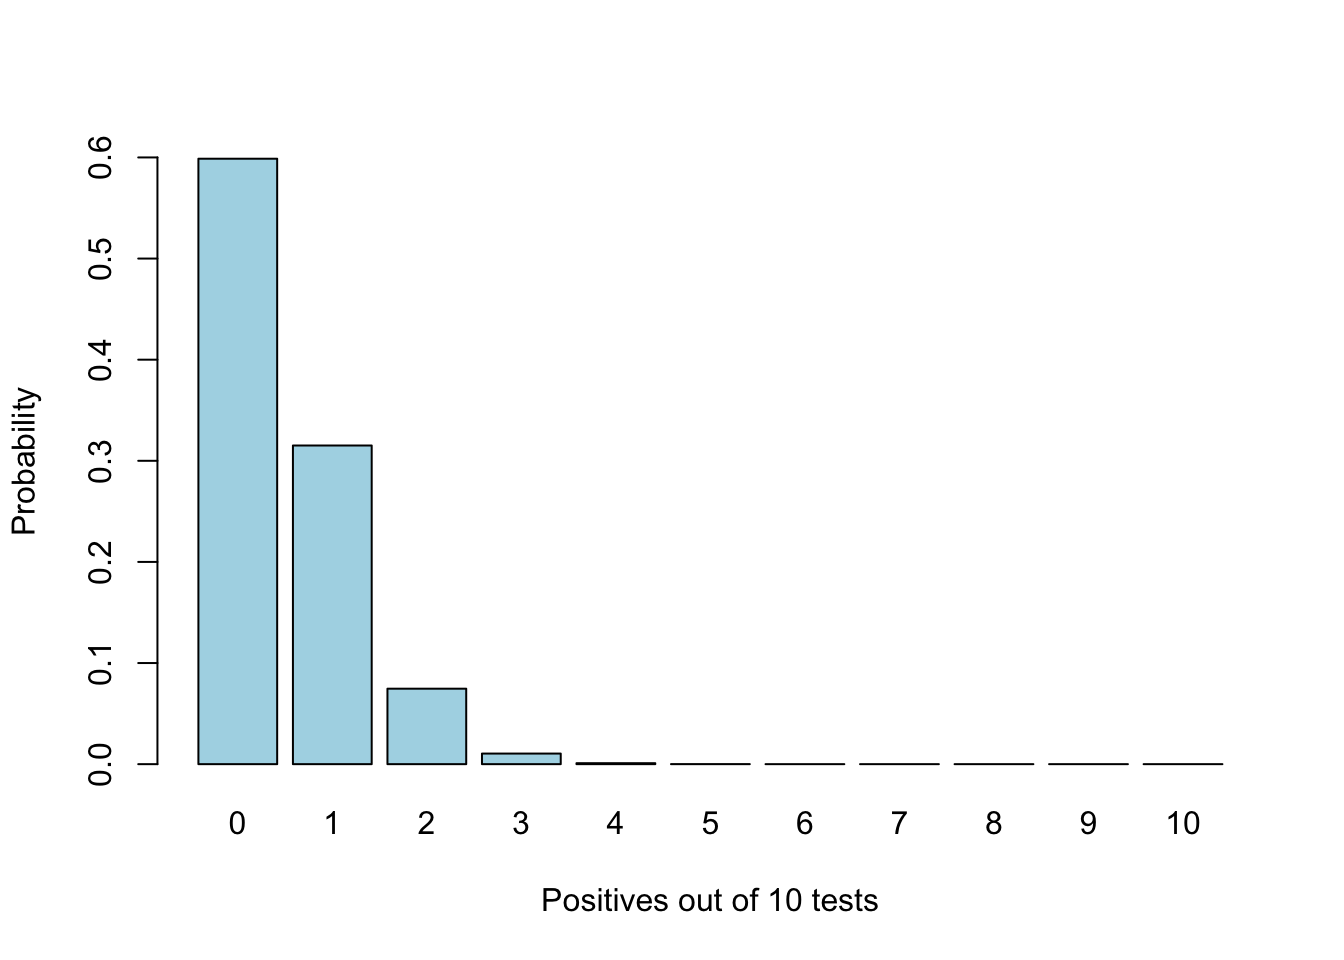
\includegraphics{Research-Design---Statistics_files/figure-latex/c7f4-1} 

}

\caption{Discrete probability distribution of the number of positive tests out of 10 trials when 5\% of the population is infected.}\label{fig:c7f4}
\end{figure}

The probability distribution shows that the most likely outcome is no positives out of 10 when the prevalence is 0.05, and the probability of each outcome decreases as the number of positives increases. That shouldn't be too surprising given that only 5\% of the population is infected. The probability distribution would look much different if 50\% of the population was infected (Figure \ref{fig:c7f5}).

\begin{figure}

{\centering 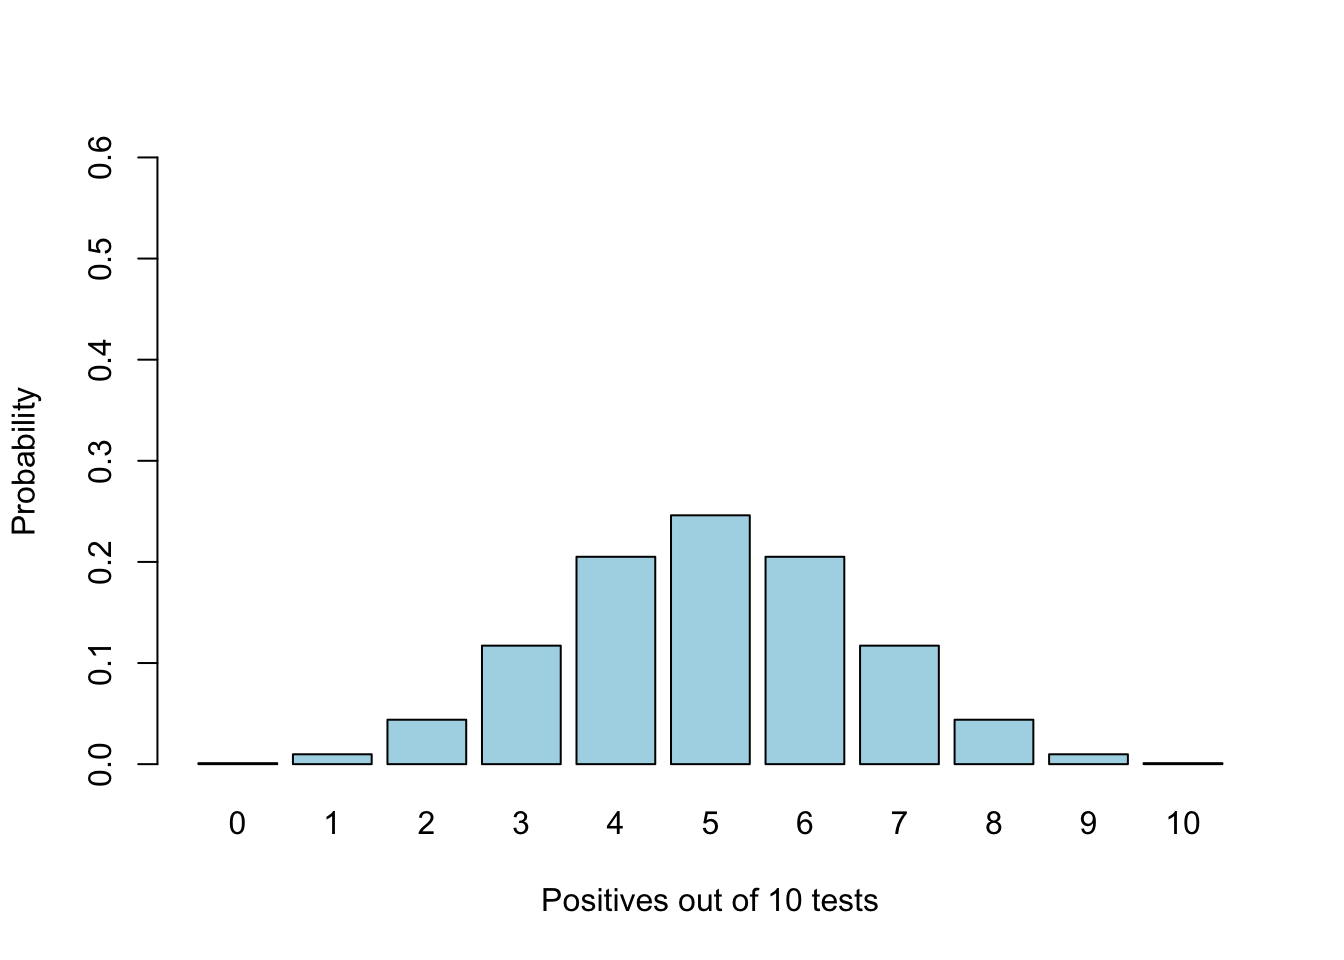
\includegraphics{Research-Design---Statistics_files/figure-latex/c7f5-1} 

}

\caption{Discrete probability distribution of the number of positive tests out of 10 trials when 50\% of the population is infected.}\label{fig:c7f5}
\end{figure}

When 50\% of the population is infected, the most likely outcome is 5 positive tests out of 10, but other values are distinctly possible due to sampling error. In fact, it's more likely than not to get a value other than 5 positives. Let's apply our \emph{not rule} to see the exact probability:

\begin{Shaded}
\begin{Highlighting}[]
\DecValTok{1} \SpecialCharTok{{-}} \FunctionTok{dbinom}\NormalTok{(}\DecValTok{5}\NormalTok{, }\DecValTok{10}\NormalTok{, }\AttributeTok{prob=}\FloatTok{0.5}\NormalTok{)}
\end{Highlighting}
\end{Shaded}

\begin{verbatim}
## [1] 0.7539062
\end{verbatim}

Here we see there's a 75\% chance of observing a value other than 5 positive tests out of 10 when the prevalence of the disease is 50\%. This is an excellent illustration of the problem of sampling error, the same sampling error that you'd expect when flipping a coin 10 times.

\paragraph{Mean for a binomial random variable}\label{mean-for-a-binomial-random-variable}

As we saw in Chapter 2, we can characterize the shape of distributions by their central tendency and variation. When examining probability distributions of random variables, central tendency is usually characterized by the mean, also known as the \textbf{expected value}. The expected value of each possible outcome \emph{X} is

\[
E[X] = \sum_{X}P(X)X
\]

Expected value is simply weighing each possible outcome of the random variable \emph{X} by its probability of occurring. Let's quantify the expected value of the number of positives out of 10 tests when the prevalence is 50\%:

\begin{Shaded}
\begin{Highlighting}[]
\CommentTok{\#create a vector of outcomes}
\NormalTok{x }\OtherTok{\textless{}{-}} \FunctionTok{c}\NormalTok{(}\DecValTok{0}\SpecialCharTok{:}\DecValTok{10}\NormalTok{)}

\CommentTok{\#sum the products of each outcome and its probability}
\FunctionTok{sum}\NormalTok{(}\FunctionTok{dbinom}\NormalTok{(}\AttributeTok{x=}\NormalTok{x, }\AttributeTok{size=}\DecValTok{10}\NormalTok{, }\AttributeTok{prob=}\FloatTok{0.5}\NormalTok{)}\SpecialCharTok{*}\NormalTok{x)}
\end{Highlighting}
\end{Shaded}

\begin{verbatim}
## [1] 5
\end{verbatim}

We see exactly what we expect. When the prevalence is 50\% and we conduct 10 tests, we expect 5 positives on average. What if the prevalence was 5\%?

\begin{Shaded}
\begin{Highlighting}[]
\FunctionTok{sum}\NormalTok{(}\FunctionTok{dbinom}\NormalTok{(}\AttributeTok{x=}\NormalTok{x, }\AttributeTok{size=}\DecValTok{10}\NormalTok{, }\AttributeTok{prob=}\FloatTok{0.05}\NormalTok{)}\SpecialCharTok{*}\NormalTok{x)}
\end{Highlighting}
\end{Shaded}

\begin{verbatim}
## [1] 0.5
\end{verbatim}

When the prevalence is 5\%, we expect 0.5 positives on average. Obviously you can't observe 0.5 positives for a discrete random variable, so you need to think about the expected value of discrete random variables as the long run outcome. That is, if you could take thousands of samples of 10 and compute the mean of the number of positives across samples, you'd expect the mean to be 0.5 positives. Remember that we can actually do that via simulation in R:

\begin{Shaded}
\begin{Highlighting}[]
\FunctionTok{set.seed}\NormalTok{(}\DecValTok{123}\NormalTok{)}

\CommentTok{\#create a vector representing 5\% infected in a population of 100}
\NormalTok{infections }\OtherTok{\textless{}{-}} \FunctionTok{c}\NormalTok{(}\FunctionTok{rep}\NormalTok{(}\DecValTok{1}\NormalTok{, }\DecValTok{5}\NormalTok{), }\FunctionTok{rep}\NormalTok{(}\DecValTok{0}\NormalTok{, }\DecValTok{95}\NormalTok{))}

\CommentTok{\#create an empty vector to store the number of positives across 1 million sims}
\NormalTok{x }\OtherTok{\textless{}{-}} \FunctionTok{rep}\NormalTok{(}\ConstantTok{NA}\NormalTok{, }\DecValTok{1000000}\NormalTok{)}

\CommentTok{\#simulate 10 tests 1 million times \& record \# positives each time}
\ControlFlowTok{for}\NormalTok{(i }\ControlFlowTok{in} \DecValTok{1}\SpecialCharTok{:}\FunctionTok{length}\NormalTok{(x)) \{}
\NormalTok{  x.trial }\OtherTok{\textless{}{-}} \FunctionTok{sample}\NormalTok{(infections, }\DecValTok{10}\NormalTok{, }\AttributeTok{replace=}\ConstantTok{TRUE}\NormalTok{)}
\NormalTok{  x[i] }\OtherTok{\textless{}{-}} \FunctionTok{sum}\NormalTok{(x.trial)}
\NormalTok{\}}

\CommentTok{\#quantify the expected value}
\FunctionTok{mean}\NormalTok{(x)}
\end{Highlighting}
\end{Shaded}

\begin{verbatim}
## [1] 0.500318
\end{verbatim}

The simulation shows that we expect 0.500351 positive tests out of 10, almost exactly the correct answer.

For binomial random variables, the mean of the probability distribution is equal to the true probability of success, so the expected value of a binomial random variable can be quantified simply as \(E(X) = np\), where \(n\) is the number of trials and \(p\) is the probability of success. For example, when we take \(n = 10\) tests from a population with \(p_{infection} = 0.05\), the expected value can be computed as \(E(X) = np=10*0.05=0.5\).

\paragraph{Variance for a binomial random variable}\label{variance-for-a-binomial-random-variable}

Recall that variance is a measure of variation in an outcome relative to the mean. The variance will be large when outcomes of the random variable can range widely around the mean, and it will be small when the outcomes show little variation around the mean. For a discrete random variable, the variance is quantified as

\[
V[X]=\sum_{X}P(X)(X-E[X])^2
\]
What does this mean? Just like we saw in the variance formula before, we're looking at how far each value of X is away from the mean, quantified as the squared difference between \(X\) and \(E[X]\). We weigh each of those squared deviations by the probability of X, \(P(X)\), and then we sum them up. Intuitively, you should see that the variance will increase as there are highly probable values of \(X\) far from the mean.

The variance formula for a binomial random variable can be simplified to the following:

\[
V[X]=np(1-p)
\]
From this formula we can see that the variance of a binomial random variable will be greatest when the probability of success is closer to 0.5. When \(p=0.5\) and \(n\) = 100, the variance is \(V[X]=100*0.5(1-0.5)=25\). Any deviation from \(p = 0.5\) leads to lower variance. For example, when \(p=0.05\) (e.g., 5\% prevalence of infection), the variance is \(V[X]=100*0.05(1-0.05)=4.75\). At the extremes, when \(p = 0\) or \(p = 1\), the variance by definition must be 0. What this means is that probability distribution for binomial random variables will be somewhat bell-shaped with long tails when the probability of success is close to 0.5, and it will become skewed as the probability distribution deviates from 0.5.

\subsection{Continuous random variables}\label{continuous-random-variables}

Discrete probability distributions are straightforward because we can quantify the probability mass for each discrete outcome in the sample space. When we test an individual for a viral infection, the outcome is either positive or negative with probabilities \(p_{positive}\) and \(p_negative\). But not all random variables are so simple. Many variables form \textbf{continuous} probability distributions, such as height, weight, air temperature, and many more. The challenge of characterizing probability distributions for continuous variables is that there's an \emph{infinite} number of potential outcomes in the sample space.

Consider the incubation period for a viral illness, which is the time between exposure to the pathogen and onset of symptoms. Incubation period is a continuous random variable because there's an infinite number of possibilities in the sample space. The incubation might be 2, 2.1, 2.15, 2.154, 2.1547 days, and so on. The probability of the incubation period being a particular value (e.g., 2.154794667 days) is 0 because there's an infinite number of possible values. If there's an infinite number of possible values in the sample space and each possibility had a non-zero probability, then the sum of the probability of all the mutually exclusive outcomes would be infinity, violating our rules of probability.

\subsubsection{Probability density function}\label{probability-density-function}

To characterize probability distributions for continuous variables, we use the concept of \textbf{probability density}. A \textbf{probability density function (pdf)} describes how probability is distributed across the possible values of a continuous random variable. Instead of assigning probabilities to individual points, the pdf reflects how ``dense'' the probability is at different values of the random variable.

To visualize this concept, we can approximate a continuous variable by discretizing the sample space into intervals. Figure \ref{fig:c7f6} shows a simulated distribution of incubation times for 10,000 individuals, grouped into bins of 0.1 days. The highlighted bin for 2.4--2.5 days contains 1,375 observations, meaning the probability mass for this interval is:

\[
\frac{1375}{10000}=0.1375
\]
The probability density is defined as the ratio of the probability mass to the bin width, in this case:

\[
\frac{0.1375}{0.1}=1.375
\]

Here we see that probability densities can be greater than 1. That's because probability density is a measure of how concentrated the probability is within a particular interval (a density!) rather than a probability of a particular observation. In this way probability density is similar to measuring human population density in a city. A city can have densities well over one person per square kilometer, even though the probability of finding one person in a randomly selected square kilometer is very low.

\begin{figure}

{\centering 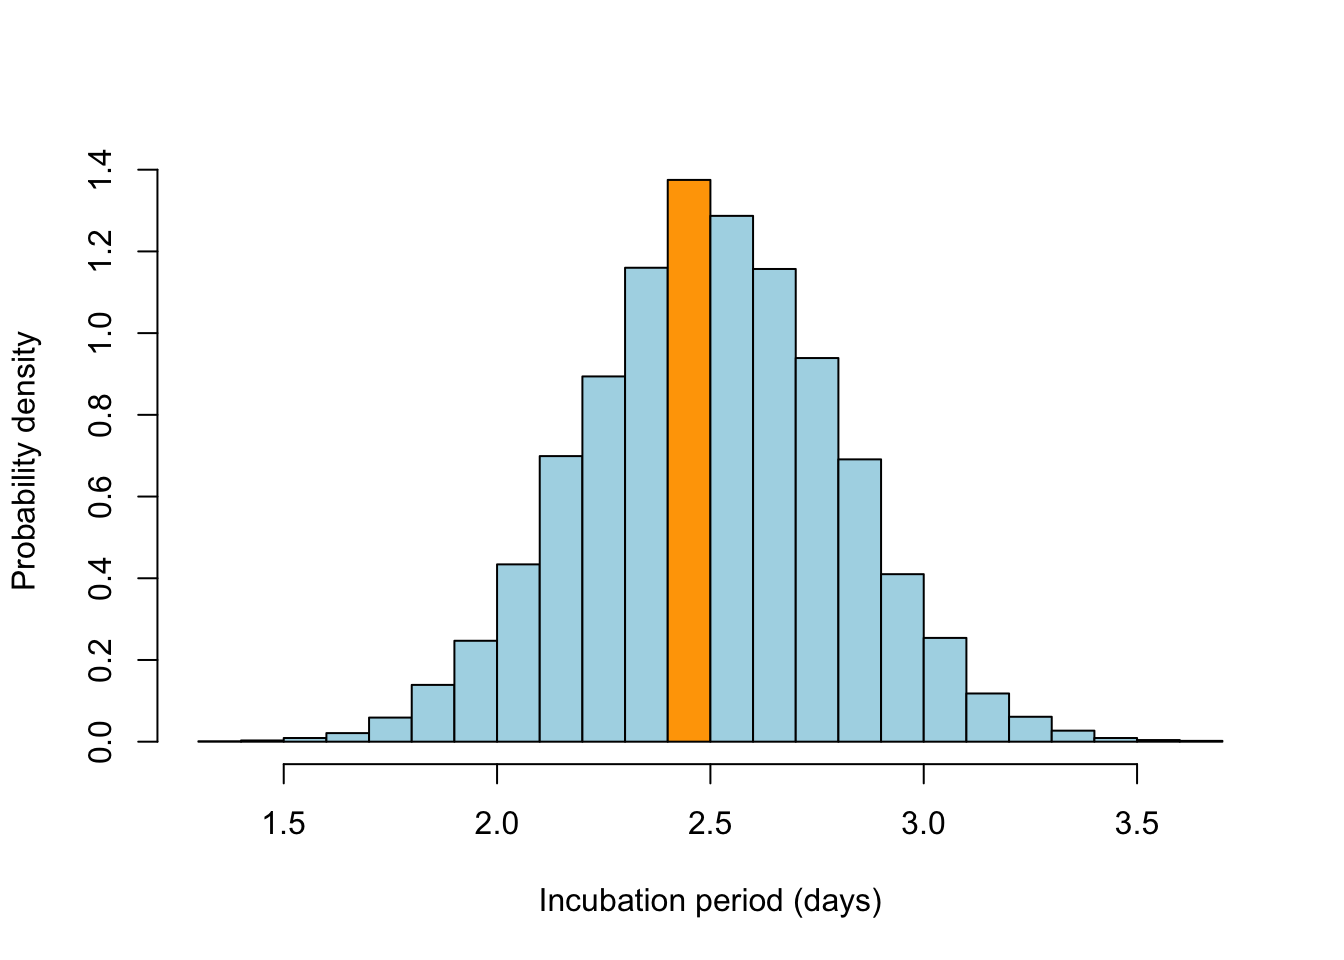
\includegraphics{Research-Design---Statistics_files/figure-latex/c7f6-1} 

}

\caption{Probability distribution of incubation period with intervals of 0.1 days.}\label{fig:c7f6}
\end{figure}

If we can quantify probability mass for a discrete interval, why do we use probability density? We use probability density because we want to describe the distribution continuously, without being constrained by arbitrary interval sizes. Narrower intervals result in smaller probability masses, approaching zero as the interval size approaches zero. The pdf allows us to describe the relative likelihood of observations without relying on a fixed bin size. Given a pdf, we can quantify the probability mass of \emph{any} interval by applying integrals from calculus, which represents the area under the curve of the pdf over the interval of interest. The total probability over the entire sample space remains one, satisfying the basic rules of probability.

\subsubsection{Normal distribution}\label{normal-distribution}

Perhaps the most well-known probability density function for a continuous random variable is the \textbf{normal distribution}, also known as a \textbf{Gaussian distribution}. The normal distribution can be used to describe any continuous variable with positive or negative values. The normal distribution is among the most recognized because many continuous variable follow a normal distribution. As we'll see, the normal distribution also tends to be important for some methods of statistical hypothesis testing.

For a normal random variable, the probability density of any value X is quantified as

\[
f(X) = \frac{1}{\sqrt{2\pi\sigma^2}} e^{-\frac{(x - \mu)^2}{2\sigma^2}}
\]
where \(f(X)\) is the probabilty density of value \(X\), \(\mu\) is the mean and \(\sigma^2\) is the variance of the random variable. This is an ugly equation, but don't fret. The main takeaway here is that a normal distribution has two parameters. The mean (\(\mu\)) controls location, and the variance (\(\sigma^2\), or standard deviation, \(\sigma\)) controls the variation or width of the normal distribution.

In R we can use the \texttt{dnorm} function to compute the probability density of \(X\) given values for \(\mu\) and \(\sigma\). For example, let's compute probability density for values between 1 and 4 days assuming incubation period follows a normal distribution with \(\mu\) = 2.5 and \(\sigma\) = 0.3 days.

\begin{figure}

{\centering 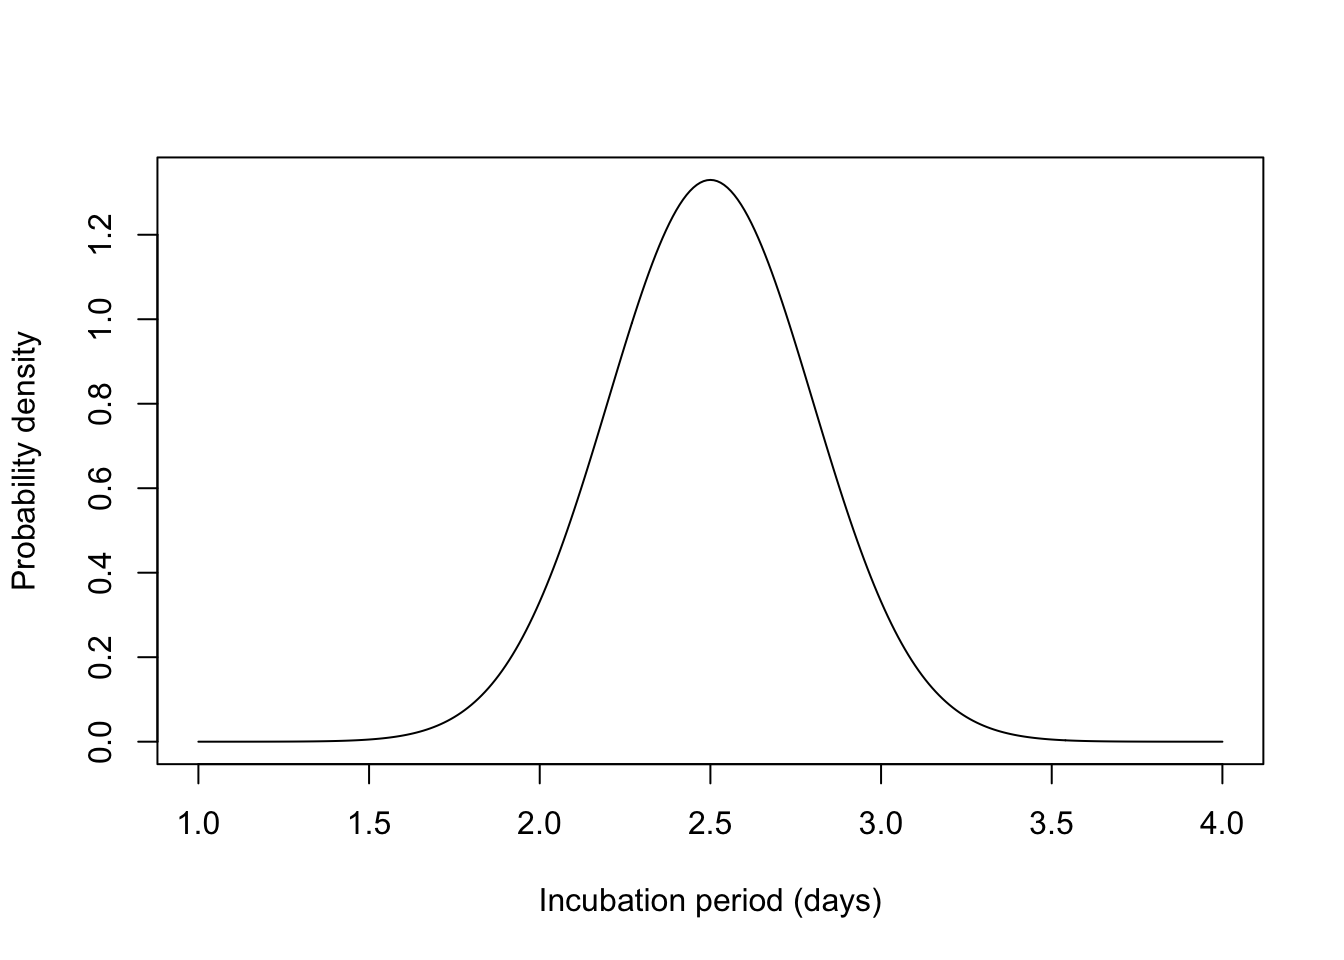
\includegraphics{Research-Design---Statistics_files/figure-latex/c7f7-1} 

}

\caption{Probability density function assuming a normal distribution of incubation period mean = 2.5 and SD = 0.3 days.}\label{fig:c7f7}
\end{figure}

Figure \ref{fig:c7f7} shows the resulting probability density function, which we can use to highlight important characteristics of the normal distribution:

\begin{enumerate}
\def\labelenumi{\arabic{enumi}.}
\tightlist
\item
  The normal distribution is bell-shaped and symmetric around the mean. In other words, the probability of incubation period being less than 2.5 days is 0.5, and the probability of incubation period being more than 2.5 days is 0.5. We can very that with the \texttt{pnorm} function, which computes the probability mass of values below a defined value when the \texttt{lower.tail} argument is \texttt{TRUE}. The probability mass greater than the defined value is computed when \texttt{lower.tail\ =\ FALSE}.
\end{enumerate}

\begin{Shaded}
\begin{Highlighting}[]
\FunctionTok{pnorm}\NormalTok{(}\FloatTok{2.5}\NormalTok{, }\AttributeTok{mean =} \FloatTok{2.5}\NormalTok{, }\AttributeTok{sd =} \FloatTok{0.3}\NormalTok{, }\AttributeTok{lower.tail=}\ConstantTok{TRUE}\NormalTok{) }\CommentTok{\#P(X\textless{}2.5)}
\end{Highlighting}
\end{Shaded}

\begin{verbatim}
## [1] 0.5
\end{verbatim}

\begin{Shaded}
\begin{Highlighting}[]
\FunctionTok{pnorm}\NormalTok{(}\FloatTok{2.5}\NormalTok{, }\AttributeTok{mean =} \FloatTok{2.5}\NormalTok{, }\AttributeTok{sd =} \FloatTok{0.3}\NormalTok{, }\AttributeTok{lower.tail=}\ConstantTok{FALSE}\NormalTok{) }\CommentTok{\#P(X\textgreater{}2.5)}
\end{Highlighting}
\end{Shaded}

\begin{verbatim}
## [1] 0.5
\end{verbatim}

The \texttt{pnorm} function is applying the integral from calculus mentioned earlier, effectively quantifying probability mass for an interval as the area under the density function curve for that interval. We can quantify probability mass for any interval in this way. For example, what's the probability that incubation period is less than 2 days?

\begin{Shaded}
\begin{Highlighting}[]
\FunctionTok{pnorm}\NormalTok{(}\DecValTok{2}\NormalTok{, }\AttributeTok{mean =} \FloatTok{2.5}\NormalTok{, }\AttributeTok{sd =} \FloatTok{0.3}\NormalTok{, }\AttributeTok{lower.tail=}\ConstantTok{TRUE}\NormalTok{) }\CommentTok{\#P(X\textless{}1.5)}
\end{Highlighting}
\end{Shaded}

\begin{verbatim}
## [1] 0.04779035
\end{verbatim}

We see there's less than a 5\% chance that incubation period is less than 2 days.

\begin{enumerate}
\def\labelenumi{\arabic{enumi}.}
\setcounter{enumi}{1}
\tightlist
\item
  The mean is the expected value of the normal distribution and specifies the central tendency of the distribution. Figure \ref{fig:c7f8} shows three normal distributions each with different means. Notice the means control where the center of the distribution is located, while the width of the distribution remains the same.
\end{enumerate}

\begin{figure}

{\centering 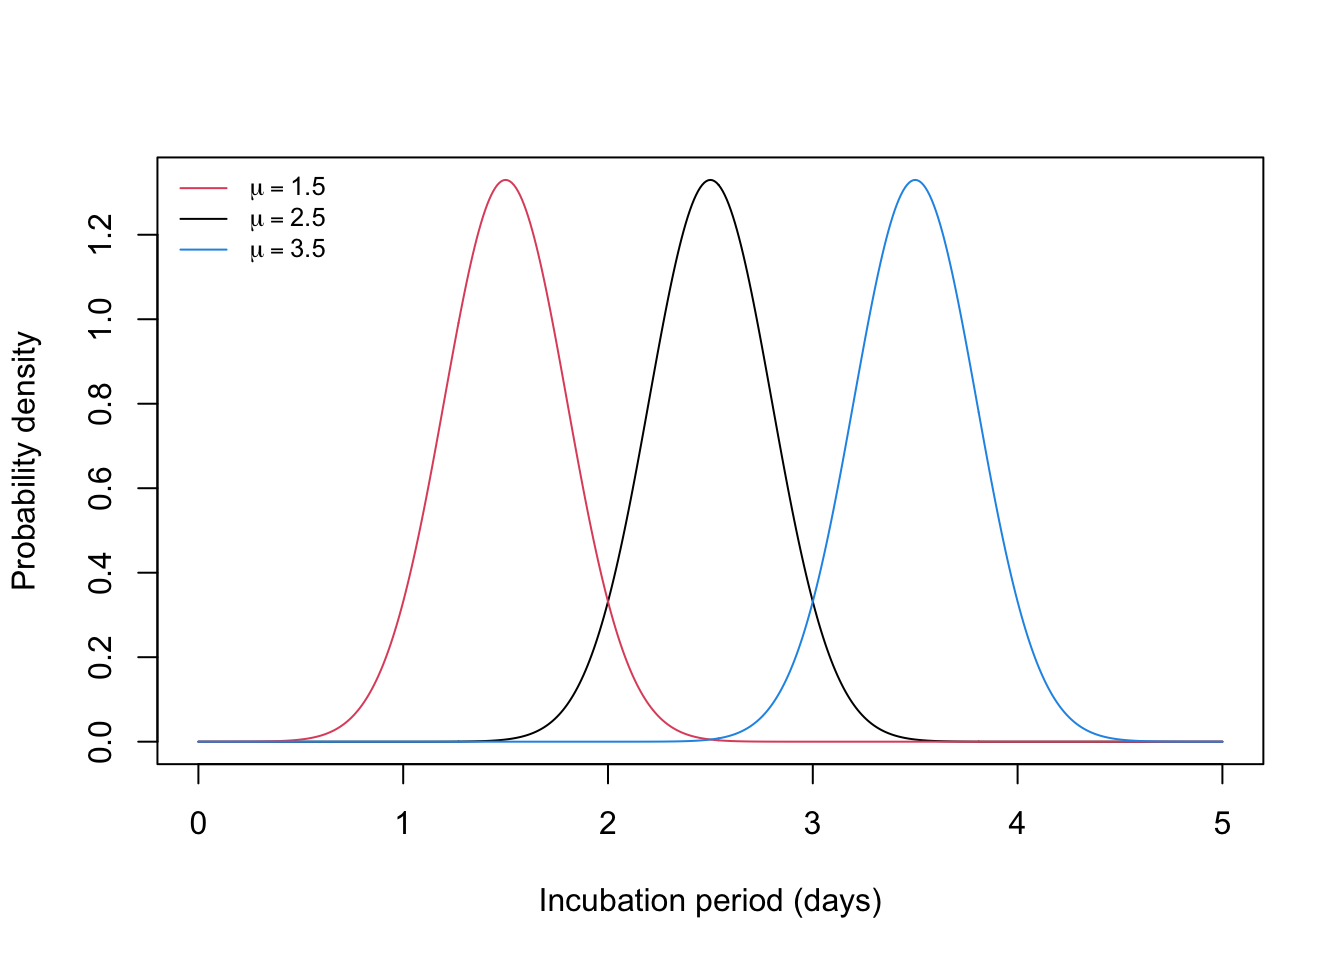
\includegraphics{Research-Design---Statistics_files/figure-latex/c7f8-1} 

}

\caption{Probability density functions with varying means but identical standard deviations.}\label{fig:c7f8}
\end{figure}

\begin{enumerate}
\def\labelenumi{\arabic{enumi}.}
\setcounter{enumi}{2}
\tightlist
\item
  The variance of a normal distribution controls the spread of the observations away from the mean, although note that unlike the binomial distribution, the variance of a normal distribution does \emph{not} depend on the value of the mean. Figure \ref{fig:c7f9} shows three normal distributions each with identical means but different standard deviations. Notice how the width of the normal distribution grows as the standard deviation increases.
\end{enumerate}

\begin{figure}

{\centering 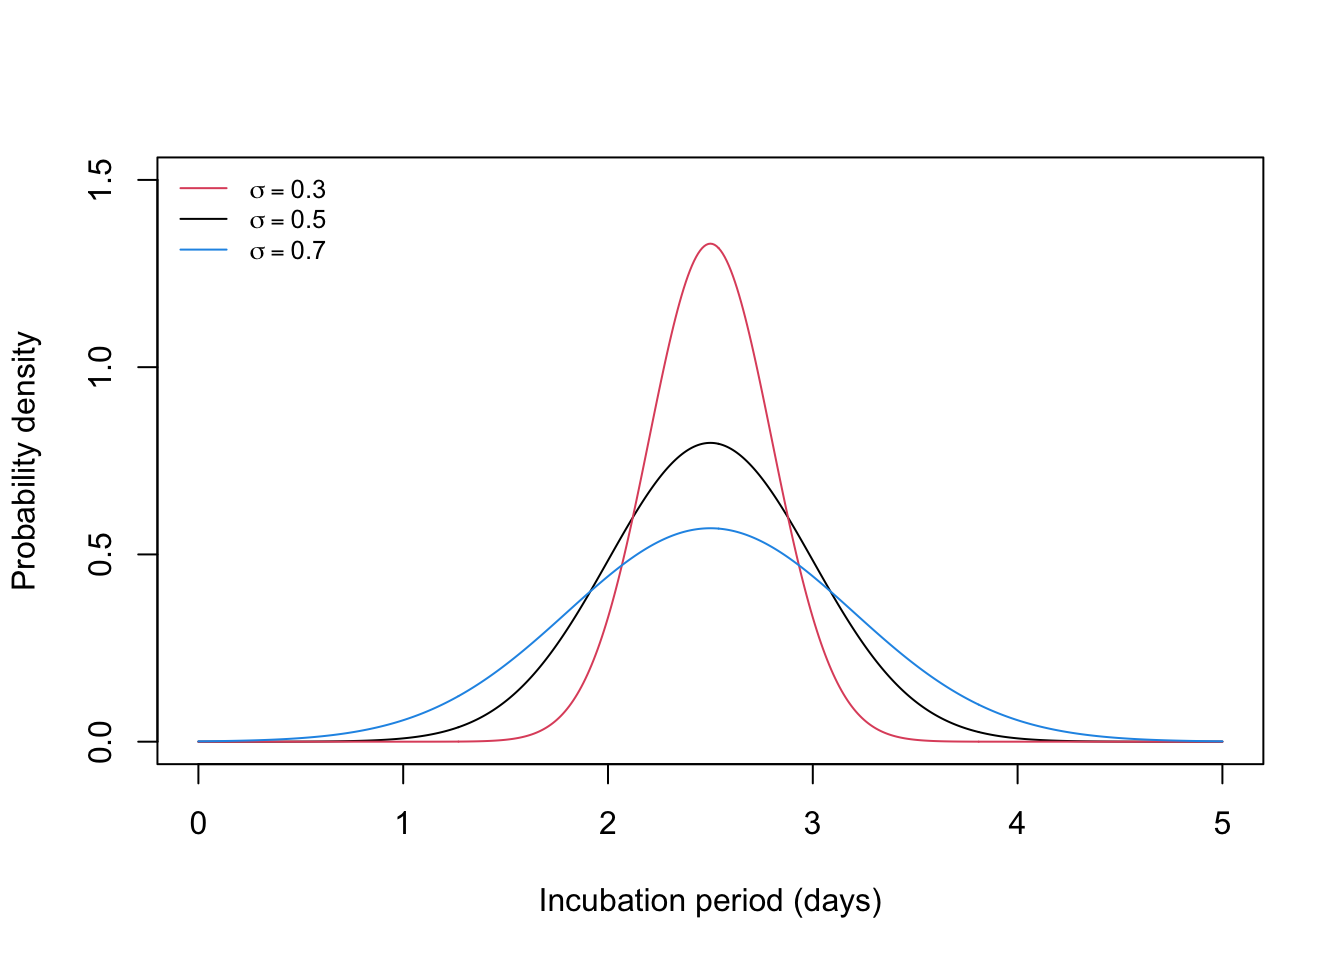
\includegraphics{Research-Design---Statistics_files/figure-latex/c7f9-1} 

}

\caption{Probability density functions with identical means but varying standard deviations.}\label{fig:c7f9}
\end{figure}

\paragraph{Probability mass and the empirical rule}\label{probability-mass-and-the-empirical-rule}

Recall that we can quantify probability mass as area under the probability density function for any interval of interest. Consider again the normal distribution with \(\mu = 2.5\) and \(\sigma = 0.3\). What's the probability that incubation period will be between 2.2 and 2.8? The interval of interest is shaded in the probability density function in Figure \ref{fig:c7f10}.

\begin{figure}

{\centering 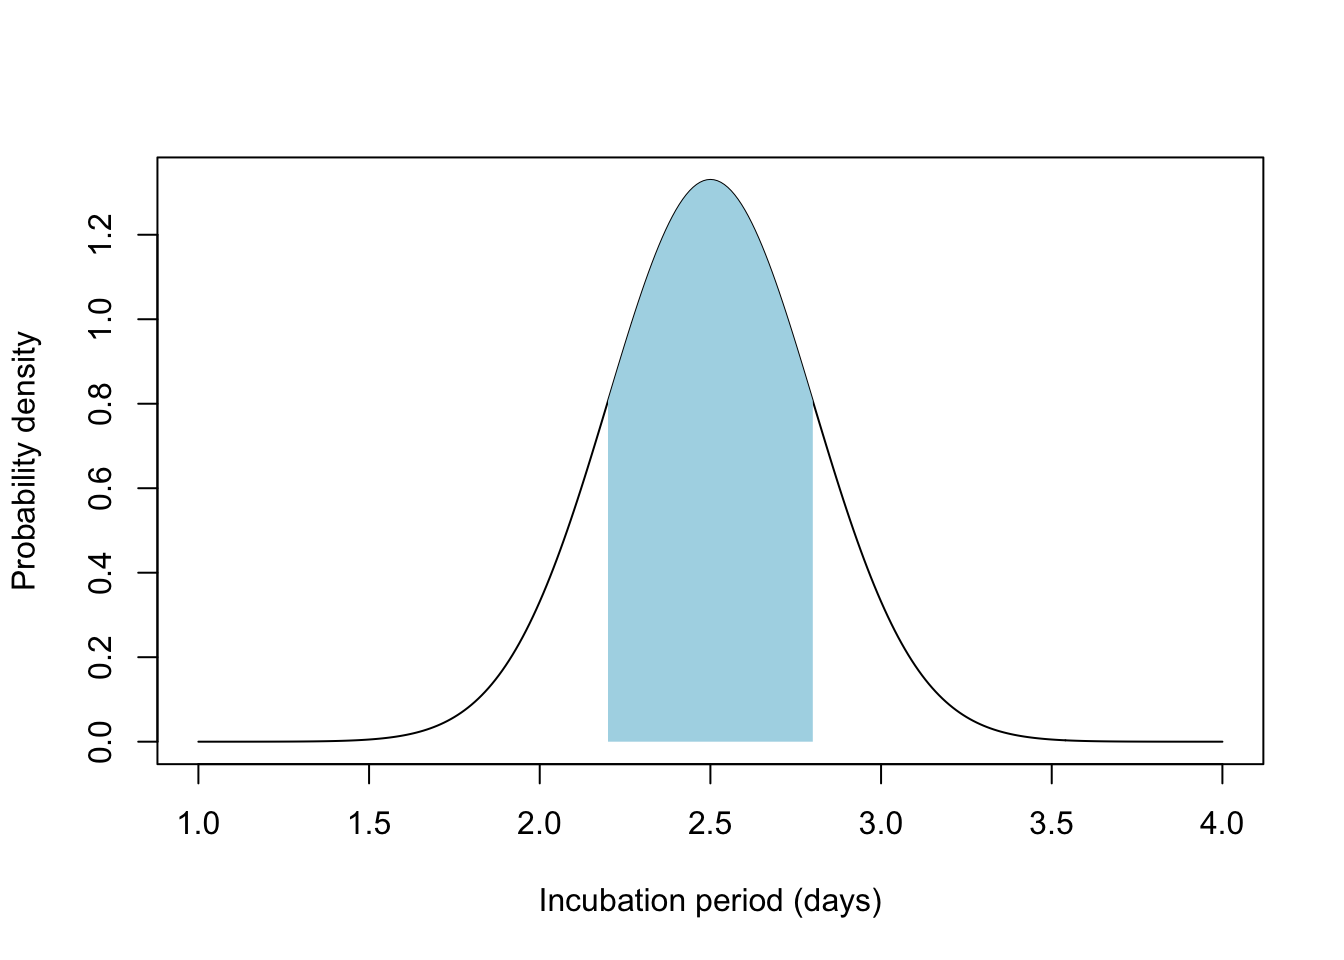
\includegraphics{Research-Design---Statistics_files/figure-latex/c7f10-1} 

}

\caption{Probability density function highlighting the interval 2.2 to 2.8}\label{fig:c7f10}
\end{figure}

We can apply the \texttt{pnorm} function to find the probability of observations between 2.2 and 2.8 as the area under the curve in that interval:

\begin{Shaded}
\begin{Highlighting}[]
\FunctionTok{pnorm}\NormalTok{(}\FloatTok{2.8}\NormalTok{, }\FloatTok{2.5}\NormalTok{, }\FloatTok{0.3}\NormalTok{, }\AttributeTok{lower.tail=}\NormalTok{T) }\SpecialCharTok{{-}} \FunctionTok{pnorm}\NormalTok{(}\FloatTok{2.2}\NormalTok{, }\FloatTok{2.5}\NormalTok{, }\FloatTok{0.3}\NormalTok{, }\AttributeTok{lower.tail=}\NormalTok{T)}
\end{Highlighting}
\end{Shaded}

\begin{verbatim}
## [1] 0.6826895
\end{verbatim}

This code asks for the probability between 2.2 and 2.8 by subtracting the cumulative probability up to 2.2 from the cumulative probability up to 2.8. We find that 68.3\% of the observations fall between 2.2 and 2.8.

How about values between 1.9 and 3.1 (Figure \ref{fig:c7f11}))?

\begin{figure}

{\centering \includegraphics{Research-Design---Statistics_files/figure-latex/c7f11-1} 

}

\caption{Probability density function highlighting the interval 2.2 to 2.8}\label{fig:c7f11}
\end{figure}

\begin{Shaded}
\begin{Highlighting}[]
\FunctionTok{pnorm}\NormalTok{(}\FloatTok{1.9}\NormalTok{, }\FloatTok{2.5}\NormalTok{, }\FloatTok{0.3}\NormalTok{, }\AttributeTok{lower.tail=}\NormalTok{F) }\SpecialCharTok{{-}} \FunctionTok{pnorm}\NormalTok{(}\FloatTok{3.1}\NormalTok{, }\FloatTok{2.5}\NormalTok{, }\FloatTok{0.3}\NormalTok{, }\AttributeTok{lower.tail=}\NormalTok{F) }
\end{Highlighting}
\end{Shaded}

\begin{verbatim}
## [1] 0.9544997
\end{verbatim}

Here I quantified \(P(X>1.9)\) and subtracted \(P(X>3.1)\), which shows us that 95.4\% of values lie between 1.9 and 3.1.

It's helpful to think about probability mass as the area under the pdf and to quantify those probabilities with the \texttt{pnorm} function, but what we've also done here is illustrate the \textbf{emprical rule}. The empirical rule is that about 68\% of the probability mass falls within 1 standard deviation of the mean (i.e., \(\mu \pm 1\sigma\) ), whereas about 95\% of the probability mass falls within 2 standard deviations of the mean (i.e., \(\mu \pm 2\sigma\) ). Figure \ref{fig:c7f12} shows the empirical rule graphically for our example normal distribution of incubation period.

\begin{figure}

{\centering \includegraphics{Research-Design---Statistics_files/figure-latex/c7f12-1} 

}

\caption{Normal probability density function showing the empirical rule, namely that about 68\% of observations are within one standard deviation of the mean, and about 95\% of observations are within two standard deviations of the mean. In this example, the mean incubation period is 2.5 and the standard deviation is 0.3.}\label{fig:c7f12}
\end{figure}

\paragraph{Standard normal distribution}\label{standard-normal-distribution}

Any combination of \(\mu\) and \(\sigma\) produces a unique normal distribution, so there's an infinite variety of possible normal distributions. However, any normal distribution can be converted to a \textbf{standard normal distribution}, which is a normal distribution with \(\mu = 0\) and \(\sigma = 1\) (Figure \ref{fig:c7f13}). Because the standard deviation is one, the values of the standard normal distribution are in units of standard deviations. The values of a standard normal distribution are denoted \(Z\), or \(Z-scores\).

\begin{figure}

{\centering \includegraphics{Research-Design---Statistics_files/figure-latex/c7f13-1} 

}

\caption{Standard normal distribution with mean = 0 and standard deviation = 1. The values Z of a standard normal distribution are in units of standard deviations away from the mean.}\label{fig:c7f13}
\end{figure}

We can convert any observation \(X\) drawn from a normal distribution to a Z-score using the following formula:

\[
Z = \frac{X-\mu}{\sigma}
\]
Consider the normal distribution of incubation period with \(\mu = 2.5\) and \(\sigma=0.3\) days. Let's say we have an observation \(X\) of 2.8 days for the incubation period. The corresponding Z-score is thus

\[
Z = \frac{X-\mu}{\sigma} =\frac{2.8-2.5}{0.3}=1 
\]
In other words, the value 2.8 days is one standard deviation above the mean. Consider another observation \(X\) of 2.05 days:

\[
Z = \frac{X-\mu}{\sigma} =\frac{2.05-2.5}{0.3}=-1.5
\]
The negative value of \(Z\) indicates the observation \(X\) is below the mean, so can say the observation of 2.05 days is 1.5 standard deviations below the mean. The standard normal distribution is perfectly symmetric around 0, so half the observations are positive and half are negative.

The standard normal distribution is useful as a common language to talk about any normal distribution, but there's also practical value that we'll encounter in statistics of converting variables to Z-scores. The process of transforming a variable to Z-scores is called \textbf{standardization}, and in R we can use the \texttt{scale} function to make the conversion. For example, here I generate a dataset of 10 values, which I then convert to z-scores:

\begin{Shaded}
\begin{Highlighting}[]
\NormalTok{x }\OtherTok{\textless{}{-}} \FunctionTok{c}\NormalTok{(}\DecValTok{0}\NormalTok{, }\DecValTok{1}\NormalTok{, }\DecValTok{3}\NormalTok{, }\DecValTok{5}\NormalTok{, }\DecValTok{6}\NormalTok{, }\DecValTok{6}\NormalTok{, }\DecValTok{7}\NormalTok{, }\DecValTok{7}\NormalTok{, }\DecValTok{9}\NormalTok{, }\DecValTok{10}\NormalTok{)}
\NormalTok{z }\OtherTok{\textless{}{-}} \FunctionTok{scale}\NormalTok{(x)}
\NormalTok{z}
\end{Highlighting}
\end{Shaded}

\begin{verbatim}
##             [,1]
##  [1,] -1.6673586
##  [2,] -1.3585885
##  [3,] -0.7410483
##  [4,] -0.1235080
##  [5,]  0.1852621
##  [6,]  0.1852621
##  [7,]  0.4940322
##  [8,]  0.4940322
##  [9,]  1.1115724
## [10,]  1.4203425
## attr(,"scaled:center")
## [1] 5.4
## attr(,"scaled:scale")
## [1] 3.238655
\end{verbatim}

The scale function returns each value \(X\) as a Z-score, and it also computes the mean (\texttt{scaled:center}) and standard deviation (\texttt{scaled:scale}). Note that if we standardize the value directly, we'd get the same Z-scores:

\begin{Shaded}
\begin{Highlighting}[]
\NormalTok{z }\OtherTok{\textless{}{-}}\NormalTok{ (x}\SpecialCharTok{{-}}\FunctionTok{mean}\NormalTok{(x))}\SpecialCharTok{/}\FunctionTok{sd}\NormalTok{(x)}
\NormalTok{z}
\end{Highlighting}
\end{Shaded}

\begin{verbatim}
##  [1] -1.6673586 -1.3585885 -0.7410483 -0.1235080  0.1852621  0.1852621  0.4940322  0.4940322
##  [9]  1.1115724  1.4203425
\end{verbatim}

\subsection{Sampling from probability distributions}\label{sampling-from-probability-distributions}

Why does any of this matter?! Well, keep in mind that when we collect data to test scientific hypotheses, we're almost always sampling from a broader population. Imagine if I'm conducting a study to estimate the mean incubation period for a viral illness. I'd love to track down every single person who has the viral illness and record the incubation, but I can't do that. Instead, we rely on sampling. We know that sampling is a stochastic, or random process. In other words, the variables that we observe should be considered \emph{random} variables, and if we sample in an unbiased way, the values of the variable we observe through sampling are drawn from a probability distribution.

What probability distribution are observations of random variables drawn from? Often we don't know with certainty! We usually have to make some assumptions, ideally informed by knowledge of your particular discipline. I've introduced two broad types of probability distributions - discrete and random - and particular probability distribution of each type, the binomial (discrete) and normal (continuous) distributions. In reality, there are many more probability distributions one can choose from, and we'll encounter some others throughout the book, but the binomial and normal distributions provide a useful starting point. They may not be a perfect fit for a particular random variable (for example, a normal distribution allows for negative values, but incubation period can't be negative), but often these distributions can be useful approximations.

\subsubsection{Simulating data from probability distributions}\label{simulating-data-from-probability-distributions}

As we've seen in previous chapters and will continue to see throughout the book, it is often useful to simulate data. Simulating data requires making an assumption about a particular probability distribution from which the simulated observations are drawn. In R, we can simulate observations from probability distributions with particular functions. For example, the \texttt{rnorm} function is used to simulate data from a normal distribution. Indeed, this is exactly how I created the simulated data in the histogram for incubation period in Figur e\ref{fig:c7f6}. I assumed a normal distribution with \(\mu = 2.5\) and \(\sigma = 0.3\) and used the \texttt{rnorm} function to randomly draw 10,000 observations from that distribution:

\begin{Shaded}
\begin{Highlighting}[]
\CommentTok{\#makes the simulated data reproducible}
\FunctionTok{set.seed}\NormalTok{(}\DecValTok{123}\NormalTok{)}

\CommentTok{\#simulate 10,000 observations}
\NormalTok{x }\OtherTok{\textless{}{-}} \FunctionTok{rnorm}\NormalTok{(}\DecValTok{10000}\NormalTok{, }\AttributeTok{mean =} \FloatTok{2.5}\NormalTok{, }\AttributeTok{sd =} \FloatTok{0.3}\NormalTok{)}

\CommentTok{\#display the first 100 observations}
\NormalTok{x[}\DecValTok{1}\SpecialCharTok{:}\DecValTok{100}\NormalTok{]}
\end{Highlighting}
\end{Shaded}

\begin{verbatim}
##   [1] 2.331857 2.430947 2.967612 2.521153 2.538786 3.014519 2.638275 2.120482 2.293944 2.366301
##  [11] 2.867225 2.607944 2.620231 2.533205 2.333248 3.036074 2.649355 1.910015 2.710407 2.358163
##  [21] 2.179653 2.434608 2.192199 2.281333 2.312488 1.993992 2.751336 2.546012 2.158559 2.876144
##  [31] 2.627939 2.411479 2.768538 2.763440 2.746474 2.706592 2.666175 2.481426 2.408211 2.385859
##  [41] 2.291588 2.437625 2.120381 3.150687 2.862389 2.163067 2.379135 2.360003 2.733990 2.474989
##  [51] 2.575996 2.491436 2.487139 2.910581 2.432269 2.954941 2.035374 2.675384 2.537156 2.564782
##  [61] 2.613892 2.349303 2.400038 2.194427 2.178463 2.591059 2.634463 2.515901 2.776680 3.115025
##  [71] 2.352691 1.807249 2.801722 2.287240 2.293597 2.807671 2.414568 2.133785 2.554391 2.458333
##  [81] 2.501729 2.615584 2.388802 2.693313 2.433854 2.599535 2.829052 2.630554 2.402221 2.844642
##  [91] 2.798051 2.664519 2.571620 2.311628 2.908196 2.319922 3.156200 2.959783 2.429290 2.192074
\end{verbatim}

Similarly, we can use the \texttt{rbinom} function to randomly draw values from a binomial distribution. For example, let's assume infection status of individuals follows a binomial distribution with \(p_{infected} = 0.05\) (5\% of individuals infected). Here's how we can draw 10,000 observations of infection status from this distribution:

\begin{Shaded}
\begin{Highlighting}[]
\FunctionTok{set.seed}\NormalTok{(}\DecValTok{123}\NormalTok{)}

\CommentTok{\#simulate 10,000 observations}
\NormalTok{x }\OtherTok{\textless{}{-}} \FunctionTok{rbinom}\NormalTok{(}\DecValTok{10000}\NormalTok{, }\AttributeTok{size =} \DecValTok{1}\NormalTok{, }\AttributeTok{prob =} \FloatTok{0.05}\NormalTok{)}

\CommentTok{\#display the first 100 observations}
\NormalTok{x[}\DecValTok{1}\SpecialCharTok{:}\DecValTok{100}\NormalTok{]}
\end{Highlighting}
\end{Shaded}

\begin{verbatim}
##   [1] 0 0 0 0 0 0 0 0 0 0 1 0 0 0 0 0 0 0 0 1 0 0 0 1 0 0 0 0 0 0 1 0 0 0 0 0 0 0 0 0 0 0 0 0 0
##  [46] 0 0 0 0 0 0 0 0 0 0 0 0 0 0 0 0 0 0 0 0 0 0 0 0 0 0 0 0 0 0 0 0 0 0 0 0 0 0 0 0 0 1 0 0 0
##  [91] 0 0 0 0 0 0 0 0 0 0
\end{verbatim}

Here we see that each observation is either a 0 (not infected) or 1 (infected). The argument \texttt{size} refers to the number of trials for each observation that you're simulating, so I simulated a single trial for each observation, resulting in 10,000 values. If you simply want to simulate the total number of infections out of 10,000 people, you could do it this way:

\begin{Shaded}
\begin{Highlighting}[]
\FunctionTok{set.seed}\NormalTok{(}\DecValTok{123}\NormalTok{)}

\CommentTok{\#simulate 10,000 observations}
\NormalTok{x }\OtherTok{\textless{}{-}} \FunctionTok{rbinom}\NormalTok{(}\DecValTok{1}\NormalTok{, }\AttributeTok{size =} \DecValTok{10000}\NormalTok{, }\AttributeTok{prob =} \FloatTok{0.05}\NormalTok{)}
\NormalTok{x}
\end{Highlighting}
\end{Shaded}

\begin{verbatim}
## [1] 484
\end{verbatim}

Here we ask for one observation of 10,000 trials, and R subsequently reports 484 infections out of the 10,000 people.

\subsubsection{Statistical notation for probabilty distributions}\label{statistical-notation-for-probabilty-distributions}

Often a standard notation is used to indicate the probability distribution from which a random variable \(X\) is drawn. Usually this is done in the following format:

\[
X\sim \text{distribution name}(\text{parameters})
\]
Here X is the particular variable of interest, and ``\textasciitilde{}'' means ``is distributed as''. The name (or symbol) of the paritcular probability distribution is then indicated outside of parentheses, and the parameters for the probability distribution are recorded in the parentheses.

For example, we will indicate a random variable \(X\) follows a normal distribution by writing

\[
X\sim \text{Normal}(\mu, \sigma)
\]

which reads ``X is distributed as a normal distribution with a mean and standard deviation''). The normal distribution of incubation period would be recorded as

\[
X \sim \text{Normal}(2.5, 0.3)
\]

which reads ``The incubation period \emph{X} is distributed as a normal distribution with \(\mu = 2.5\) and \(\sigma = 0.3\)

For a binomial distribution, the notation looks like this:

\[
X\sim \text{Binomial}(n, p)
\]
where \(X\) is the number of successes of the random variable, \(n\) is the number of trials and \(p\) is the probability of success. So, a binomial distribution for infection status of 10,000 people with 5\% prevalence should be notated as

\[
X\sim \text{Binomial}(10000, 0.05)
\]
If you are drawing just a single trial for a binomial outcome, you can specify 1 for \(n\), or you can indicate the random variable has a Bernouilli distribution, which as you might recall, is simply a binomial distribution with \(n = 1\):

\[
X\sim \text{Bernoulli}(0.05)
\]

\chapter{Estimation with frequentist inference}\label{estimation-with-frequentist-inference}

Now that we have some basic principles of probability under our belt, we can turn our attention to the fundamental problem of inferential statistics: estimating parameter values from samples and characterizing uncertainty about our estimates. Having some basic understanding of probability was essential to explore the issues related to estimation, precisely because the language in which we will characterize uncertainty about parameter estimates \emph{is} probability.

To keep things simple, we will explore the foundational principles of estimation in the context of the scientific problem we started to look at last chapter: estimating the prevalence of a disease in a population. We will use this example to develop the principles of estimation with different philosophies of inference, namely the frequentist and Bayesian approaches. Those terms should ring a bell from last chapter, as they represent the two different definitions of probability that we looked at.

Statistics education has been dominated by the frequentist approach. And there's good reason for that! Much of the scientific literature is dominated by the frequentist approach. In a way the situation has become a positive feedback loop. Frequentist methods are used by many (most?) professional scientists because those are the methods they are taught, and statistics instructors teach frequentist methods because those are the methods that are used. But Bayesian inference is being used more and more in the scientific literature, and for good reasons. Suffice to say that I think it's time to start teaching both approaches to inference. We'll start with the frequentist approach over the next two chapters, and then turn to Bayesian inference in the next chapter.

\section{Frequentist estimates are point estimates}\label{frequentist-estimates-are-point-estimates}

Recall the scenario. We have a population of 10,000 people, and we need to estimate the prevalence of a disease to determine if public health interventions will be enforced. Those interventions will be enforced if the prevalence is 10\% or greater. We still assume our test is perfect, but we don't have the time or resources to test all 10,000 people, so will randomly sample individuals for testing. We'll also assume that anyone who is randomly selected will comply with the test. I know, these aren't realistic assumptions, but it's useful to make simplifying assumptions to develop first principles.

OK, let's further assume that we randomly sample \(N = 100\) people for testing. Out of the 100 tests, we find 8 positives and 92 negatives. Based on this single sample, we \textbf{estimate} the prevalence of the infection as

\[
\hat{p}_{infected}=\frac{8}{100}=0.08
\]

In other words, based on our sample we estimate that 8\% of the population is infected. \emph{Estimate} is a critical word here because we truly don't know what the actual prevalence of the infection is. We are trying to infer the true prevalence - that is, the parameter value - from a sample of data.

In frequentist inference, we try to draw conclusions about parameters in exactly this way. Frequentist inference assumes at the start that there is some true parameter value. We take a sample of data, and we estimate the parameter(s) of interest with the sample. Those parameter estimates are \textbf{point estimates}, in that they represent the single best estimate of the parameters of interest.

Because the frequentist approach assumes there is a single true parameter value, there's no way we can talk probabilisticaly about pramater values. For example, one might be tempted to ask ``How probable is it that the prevalence of the infection is at least 10\% given our sample of 8 of 100 infected?''. In other words, we might want to know the conditional probability \(P(p\geq0.1|\hat{p}=\frac{8}{100}=0.08)\). But from a frequentist perspective, this doesn't make sense. The true prevalence of the infection is either greater than 0.1 or not regardless of the data we observe in our sample. The parameter \(p\) is completely fixed.

OK, but what are we supposed to make of our point estimate that 8\% of the population is infected? Is it a good estimate or not? To interrogate the quality of an estimate with frequentist inference, we need to dig deeper and examine the concept of a sampling distribution.

\section{Sampling distributions}\label{sampling-distributions}

The key element of frequentist inference is that it considers an estimate from a single sample to be only one of many possible outcomes. Just imagine repeating the sampling process over and over again. Every new sample of 100 tests will produce varying point estimates becuase of samplign error. We estimated 8\% of the population is infected based on our single sample, but if we were to take another random sample, maybe we'd find the estimate is 9\%, or 6\%, or 11\%. In other words, frequentist estimates are random variables!

When we estimate a parameter with a random sample, is it possible that some estimates are more likely than others? Absolutely. Because the estimate is a random variable, it can be described by a probability distribution. In frequentist statistics, the probability distribution used to describe a sample estimate is called the \textbf{sampling distribution}.

Let's assume that the true prevalence of the disease is 11\% in our population of 10,000 people. If that's the case, how likely is it that the estimated prevalence from a sample of 100 people will be 8\%, as we saw in our sample? In probability terms, what is \(P(\hat{p}=\frac{8}{100}=0.08|p=0.11)\). You might recognize that in this case, the estimated prevalence \(P(\hat{p}\) is a binomial random variable, so we can quantify this probability with the binomial equation:

\[
P(X = 8) = \binom{100}{8} 0.11^8 (1 - 0.11)^{100 - 8}=0.088
\]

Of course we can quantify this easily in R:

\begin{Shaded}
\begin{Highlighting}[]
\FunctionTok{dbinom}\NormalTok{(}\AttributeTok{x =} \DecValTok{8}\NormalTok{, }\AttributeTok{size =} \DecValTok{100}\NormalTok{, }\AttributeTok{prob =} \FloatTok{0.11}\NormalTok{)}
\end{Highlighting}
\end{Shaded}

\begin{verbatim}
## [1] 0.0880522
\end{verbatim}

So we see that when we take a random sample of 100 people from a population with a true prevalence of 11\%, the probability of our point estimate being 8\% is 0.088. How does that compare to other possible values of the point estimate? Well, we can easily compute the probability of all possible outcomes for the number of positive tests and then plot the resulting distribution (Figure \ref{fig:c8f1}):

\begin{Shaded}
\begin{Highlighting}[]
\FunctionTok{library}\NormalTok{(ggplot2)}

\CommentTok{\#all possible values of positive tests out of N = 100}
\NormalTok{x }\OtherTok{\textless{}{-}} \FunctionTok{seq}\NormalTok{(}\AttributeTok{from =} \DecValTok{0}\NormalTok{, }\AttributeTok{to =} \DecValTok{100}\NormalTok{, }\AttributeTok{by =} \DecValTok{1}\NormalTok{)}

\CommentTok{\#probability of each outcome assuming prevalence is 11\%}
\NormalTok{p.hat }\OtherTok{\textless{}{-}} \FunctionTok{dbinom}\NormalTok{(}\AttributeTok{x =}\NormalTok{ x, }\AttributeTok{size =} \DecValTok{100}\NormalTok{, }\AttributeTok{prob =} \FloatTok{0.11}\NormalTok{)}

\CommentTok{\#combine into a data frame}
\NormalTok{d }\OtherTok{\textless{}{-}} \FunctionTok{cbind.data.frame}\NormalTok{(x, p.hat)}

\CommentTok{\#plot the sampling distribution}
\FunctionTok{ggplot}\NormalTok{(d, }\FunctionTok{aes}\NormalTok{(}\AttributeTok{x =}\NormalTok{ x, }\AttributeTok{y =}\NormalTok{ p.hat)) }\SpecialCharTok{+}
  \FunctionTok{geom\_col}\NormalTok{(}\AttributeTok{width =} \DecValTok{1}\NormalTok{, }\AttributeTok{fill =} \StringTok{"steelblue"}\NormalTok{, }\AttributeTok{color =} \StringTok{"black"}\NormalTok{) }\SpecialCharTok{+} 
  \FunctionTok{labs}\NormalTok{(}\AttributeTok{x =} \StringTok{"Number of positives out of N = 100"}\NormalTok{, }\AttributeTok{y =} \StringTok{"Probability"}\NormalTok{) }\SpecialCharTok{+}
  \FunctionTok{xlim}\NormalTok{(}\DecValTok{0}\NormalTok{,}\DecValTok{30}\NormalTok{) }\SpecialCharTok{+}
  \FunctionTok{theme\_classic}\NormalTok{()}
\end{Highlighting}
\end{Shaded}

\begin{figure}

{\centering \includegraphics[width=0.7\linewidth]{Research-Design---Statistics_files/figure-latex/c8f1-1} 

}

\caption{Sampling distribution of the estimated prevalence of infection based on a sample of N = 100 individuals from a population where the true prevalence of the infection is 11\%.}\label{fig:c8f1}
\end{figure}

The resulting probability distribution (Figure \ref{fig:c8f1}) shows the probability of each possible point estimate for the prevalence of the infection when we take a random sample of N = 100 from a population where the \emph{true} prevalence is 8\%. This is a \emph{sampling distribution}! Sampling distributions show the probability distribution of all possible values for an \emph{estimate} of a parameter when we take a random sample from the target population.

This is an extremely important concept. I have tried to make the case that the primary reason we need statistics is to guide decision-making about hypotheses in light of uncertainty. From a frequentist perspective, \textbf{the sampling distribution is an illustration of uncertainty about estimates taken from samples.} In this case, it shows us that when we take a random sample of 100 people, we won't necessarily find 11 positives (to give us an estimate of 11\% prevalence) even if the true prevalence of the disease is 11\%. It's certainly possible to get an estimate of 11\% from a sample of N = 100, but it's almost just as likely to get an estimate of 10\%, or 12\%. Fundamentally these deviations in our estimates from the true parameter value are caused by random sampling error.

\subsection{Sampling distributions are centered on the true parameter value}\label{sampling-distributions-are-centered-on-the-true-parameter-value}

One thing you should observe in the sampling distribution in Figure \ref{fig:c8f1} is that the distribution is centered on the true parameter value, 11\%. That is a feature of sampling distributions. The expected value of a sampling distribution (the mean) \emph{is} the true parameter value.

Now, you might be tempted to claim that our estimated prevalence of 8\% is an inaccurate estimate. But that's not quite correct. When judging the accuracy of a parameter estimate from a frequentist perspective, you have to think about the distribution of possible estimates (the sampling distribution) rather than the single estimate you observed. Frequentist estimation is based on the idea of long-run frequencies of outcomes based on many random samples. In practice you only observe one, and because of sampling error, your one estimate is very likely to deviate from the truth. But accuracy of an estimator is judged on the expected value of the estimates, not the single estimate you observed.

This is where things get tricky for frequentist estimation. You have a single estimate in hand, but to judge the accuracy of that estimate, you have to think about the collection of possible, yet unobserved estimates that you would see if you repeated your sampling many times. It's an abstract idea! Our single estimate of 8\% is indeed lower than the truth, but if you conducted sampling over and over again, you would see some estimates that are greater than the truth too. If estimates were consistently lower than the truth, then the estimates would indeed be biased.

I'm sure your wondering, ``If I can't actually observe the sampling distribution, how do I know if my single estimate is accurate?''. Good question! To judge the accuracy of your estimator, you really have to focus on aspects of the sampling design, namely the degree to which the observations you drew from the population were a random selection. Random sampling ensures that estimates - on average, across many samples - will be unbiased. In practice, there's nothing that we can quantify based on the concept of a sampling distribution that will tell us if your estimate is biased or not. To judge accuracy of estimates, you have to assess the sampling design, and especially assess whether the observations are a random sample.

\subsection{Sampling distributions allow us to estimate precision}\label{sampling-distributions-allow-us-to-estimate-precision}

Sampling distributions are abstract and can't tell us much about whether a single estimate is biased or not, but they can tell us a lot about the precision of our estimates. Indeed, the width of the sampling distribution is a measure of precision. In our example, we can see there's a reasonable chance of seeing anywhere from 5-16 positives out of 100 tests when the true prevalence is 11\%. This variation is analogous to the variation in the number of heads you expect to see out of 10 flips of a fair coin. Although you expect 5 heads, you wouldn't be surprised to get 3, or 6, or 7 heads. In the same respect, we shouldn't be too surprised to see an estimated prevalence of 8\% from a sample of N = 100 when the true prevalence is 11\%. That variation is a feature of the sampling process, and it gets to the heart of uncertainty. When we sample from populations, there is random error in the outcome, and the width of the sampling distribution illustrates the uncertainty we should feel when we consider whether our sample estimate is any good. The wider the sampling distribution, the more uncertainty, and the less confidence we should feel about our estimate being close to the truth.

What factors affect the precision of estimates as represented by the width of the sampling distribution? Let's look at two: the sample size and variance.

\subsubsection{Sample size affects precision}\label{sample-size-affects-precision}

We previously identified sample size as one of the key drivers of precision. With the sampling distribution concept, we can interrogate that idea more precisely (pun intended!). We will continue assuming that the true prevalence of the disease is 11\%, but we're not going to change the size of the sample that we draw from the population to estimate the prevalence. Let's construct sampling distributions where the sample size is 10, 100, or 1000 people:

\begin{Shaded}
\begin{Highlighting}[]
\CommentTok{\#all possible values of positive tests}
\NormalTok{x10 }\OtherTok{\textless{}{-}} \FunctionTok{seq}\NormalTok{(}\AttributeTok{from =} \DecValTok{0}\NormalTok{, }\AttributeTok{to =} \DecValTok{10}\NormalTok{, }\AttributeTok{by =} \DecValTok{1}\NormalTok{)}
\NormalTok{x100 }\OtherTok{\textless{}{-}} \FunctionTok{seq}\NormalTok{(}\AttributeTok{from =} \DecValTok{0}\NormalTok{, }\AttributeTok{to =} \DecValTok{100}\NormalTok{, }\AttributeTok{by =} \DecValTok{1}\NormalTok{)}
\NormalTok{x1000 }\OtherTok{\textless{}{-}} \FunctionTok{seq}\NormalTok{(}\AttributeTok{from =} \DecValTok{0}\NormalTok{, }\AttributeTok{to =} \DecValTok{1000}\NormalTok{, }\AttributeTok{by =} \DecValTok{1}\NormalTok{)}

\CommentTok{\#probability of each outcome assuming prevalence is 11\%}
\NormalTok{p.hat10 }\OtherTok{\textless{}{-}} \FunctionTok{dbinom}\NormalTok{(}\AttributeTok{x =}\NormalTok{ x10, }\AttributeTok{size =} \DecValTok{10}\NormalTok{, }\AttributeTok{prob =} \FloatTok{0.11}\NormalTok{)}
\NormalTok{p.hat100 }\OtherTok{\textless{}{-}} \FunctionTok{dbinom}\NormalTok{(}\AttributeTok{x =}\NormalTok{ x100, }\AttributeTok{size =} \DecValTok{100}\NormalTok{, }\AttributeTok{prob =} \FloatTok{0.11}\NormalTok{)}
\NormalTok{p.hat1000 }\OtherTok{\textless{}{-}} \FunctionTok{dbinom}\NormalTok{(}\AttributeTok{x =}\NormalTok{ x1000, }\AttributeTok{size =} \DecValTok{1000}\NormalTok{, }\AttributeTok{prob =} \FloatTok{0.11}\NormalTok{)}

\CommentTok{\#combine into a data frame}
\NormalTok{d10 }\OtherTok{\textless{}{-}} \FunctionTok{cbind.data.frame}\NormalTok{(}\AttributeTok{n =} \DecValTok{10}\NormalTok{, }\AttributeTok{p.hat =}\NormalTok{ x10}\SpecialCharTok{/}\DecValTok{10}\NormalTok{, }\AttributeTok{prob =}\NormalTok{ p.hat10)}
\NormalTok{d100 }\OtherTok{\textless{}{-}} \FunctionTok{cbind.data.frame}\NormalTok{(}\AttributeTok{n =} \DecValTok{100}\NormalTok{, }\AttributeTok{p.hat =}\NormalTok{ x100}\SpecialCharTok{/}\DecValTok{100}\NormalTok{, }\AttributeTok{prob =}\NormalTok{ p.hat100)}
\NormalTok{d1000 }\OtherTok{\textless{}{-}} \FunctionTok{cbind.data.frame}\NormalTok{(}\AttributeTok{n =} \DecValTok{1000}\NormalTok{, }\AttributeTok{p.hat =}\NormalTok{ x1000}\SpecialCharTok{/}\DecValTok{1000}\NormalTok{, }\AttributeTok{prob =}\NormalTok{ p.hat1000)}
\NormalTok{d\_all }\OtherTok{\textless{}{-}} \FunctionTok{rbind}\NormalTok{(d10, d100, d1000)}
\end{Highlighting}
\end{Shaded}

And now we can plot the sampling distributions:

\begin{Shaded}
\begin{Highlighting}[]
\CommentTok{\#plot the sampling distribution}
\FunctionTok{ggplot}\NormalTok{(d\_all, }\FunctionTok{aes}\NormalTok{(}\AttributeTok{x =}\NormalTok{ p.hat, }\AttributeTok{y =}\NormalTok{ prob)) }\SpecialCharTok{+}
  \FunctionTok{geom\_col}\NormalTok{(}\AttributeTok{data =}\NormalTok{ d\_all[d\_all}\SpecialCharTok{$}\NormalTok{n }\SpecialCharTok{==} \DecValTok{10}\NormalTok{, ], }
           \AttributeTok{fill =} \StringTok{"steelblue"}\NormalTok{, }\AttributeTok{color =} \StringTok{"black"}\NormalTok{, }\AttributeTok{width =} \FloatTok{0.1}\NormalTok{) }\SpecialCharTok{+}
  \FunctionTok{geom\_col}\NormalTok{(}\AttributeTok{data =}\NormalTok{ d\_all[d\_all}\SpecialCharTok{$}\NormalTok{n }\SpecialCharTok{==} \DecValTok{100}\NormalTok{, ], }
           \AttributeTok{fill =} \StringTok{"steelblue"}\NormalTok{, }\AttributeTok{color =} \StringTok{"black"}\NormalTok{, }\AttributeTok{width =} \FloatTok{0.01}\NormalTok{) }\SpecialCharTok{+}
  \FunctionTok{geom\_col}\NormalTok{(}\AttributeTok{data =}\NormalTok{ d\_all[d\_all}\SpecialCharTok{$}\NormalTok{n }\SpecialCharTok{==} \DecValTok{1000}\NormalTok{, ], }
           \AttributeTok{fill =} \StringTok{"steelblue"}\NormalTok{, }\AttributeTok{color =} \StringTok{"black"}\NormalTok{, }\AttributeTok{width =} \FloatTok{0.001}\NormalTok{) }\SpecialCharTok{+}
  \FunctionTok{facet\_wrap}\NormalTok{(}\SpecialCharTok{\textasciitilde{}}\NormalTok{ n, }\AttributeTok{ncol =} \DecValTok{1}\NormalTok{, }\AttributeTok{scales =} \StringTok{"free"}\NormalTok{,}
             \AttributeTok{labeller =} \FunctionTok{labeller}\NormalTok{(}\AttributeTok{n =} \ControlFlowTok{function}\NormalTok{(x) }\FunctionTok{paste}\NormalTok{(}\StringTok{"N ="}\NormalTok{, x)))}\SpecialCharTok{+}
  \FunctionTok{labs}\NormalTok{(}
    \AttributeTok{x =} \StringTok{"Estimated proportion of positives"}\NormalTok{, }
    \AttributeTok{y =} \StringTok{"Probability"}\NormalTok{, }
\NormalTok{  ) }\SpecialCharTok{+}
  \FunctionTok{theme\_classic}\NormalTok{() }\SpecialCharTok{+} 
  \FunctionTok{theme}\NormalTok{(}\AttributeTok{strip.background =} \FunctionTok{element\_rect}\NormalTok{(}\AttributeTok{fill =} \StringTok{"gray"}\NormalTok{, }\AttributeTok{color =} \StringTok{"black"}\NormalTok{), }
        \AttributeTok{strip.text =} \FunctionTok{element\_text}\NormalTok{(}\AttributeTok{color =} \StringTok{"black"}\NormalTok{, }\AttributeTok{size =} \DecValTok{11}\NormalTok{))}
\end{Highlighting}
\end{Shaded}

\begin{figure}

{\centering \includegraphics[width=0.7\linewidth]{Research-Design---Statistics_files/figure-latex/c8f2-1} 

}

\caption{Sampling distributions of the estimated prevalence of infection based on samples of size N = 10, 100, and 1000 individuals from a population where the true prevalence of the infection is 11\%.}\label{fig:c8f2}
\end{figure}

What do we notice about the sampling distributions under different sample sizes in Figure \ref{fig:c8f2}? First, each sampling distribution remains centered on the true parameter value of 11\% prevalence. The point estimate of a parameter remains an unbiased estimate of the parameter no matter the sample size. In other words, sample size has no effect on the \emph{accuracy} of estimates.

Second, as the sample size increases, the width of the sampling distribution decreases. We expect the estimated prevalence to change much more from sample to sample when the sample size is 10 than when it is 100 or 1000. Greater sample sizes lead to more precise estimates. This should make sense. After all, if you increase the sample size all the way to the size of the target population, there would be no variation at all in estimates from sample to sample.

The \textbf{Law of Large Numbers} states this explicitly, that as the sample size \(N\) increases, the point estimate ultimately converges on the true parameter value. Let's simulate this process to get a good handle on it. Remember that we assumed a target population of 10,000 individuals. Below we will create a dataset of 10000 individuals with infection status classified as 1 (infected) or 0 (not infected), where 11\% of the population is infected:

\begin{Shaded}
\begin{Highlighting}[]
\CommentTok{\#create infection status for 10000 people with 11\% infected }
\NormalTok{status }\OtherTok{\textless{}{-}} \FunctionTok{c}\NormalTok{(}\FunctionTok{rep}\NormalTok{(}\DecValTok{1}\NormalTok{, }\DecValTok{1100}\NormalTok{), }\FunctionTok{rep}\NormalTok{(}\DecValTok{0}\NormalTok{, }\DecValTok{8900}\NormalTok{))}

\CommentTok{\#randomly order the observations }
\FunctionTok{set.seed}\NormalTok{(}\DecValTok{124}\NormalTok{)}
\NormalTok{status }\OtherTok{\textless{}{-}} \FunctionTok{sample}\NormalTok{(status, }\AttributeTok{replace=}\ConstantTok{FALSE}\NormalTok{) }
\FunctionTok{head}\NormalTok{(status)}
\end{Highlighting}
\end{Shaded}

\begin{verbatim}
## [1] 0 1 0 0 0 0
\end{verbatim}

\begin{Shaded}
\begin{Highlighting}[]
\CommentTok{\#confirm the proportion infected is 11\% }
\FunctionTok{mean}\NormalTok{(status)}
\end{Highlighting}
\end{Shaded}

\begin{verbatim}
## [1] 0.11
\end{verbatim}

Now let's quantify the point estimate for the proportion infected as we increase the sample size from \(N = 1\) to \(N = 10000\). To get a sense for this, we can see above that the first individual is not infected (\texttt{status} = 0), so based on that individual with a sample size of \(N = 1\), the estimated prevalence is 0\%. Then we look at the second individual, who is infected (\texttt{status} = 1), making the point estimate \(\hat{p}=\frac{1}{2}=0.5\) based on \(N = 2\). The third individual is not infected, making the point estimate \(\hat{p}=\frac{1}{3}=0.33\), and so on. We can compute the point estimate for each individual observation with the code below:

\begin{Shaded}
\begin{Highlighting}[]
\CommentTok{\#creates the cumulative sum from each observation}
\NormalTok{status.cumsum }\OtherTok{\textless{}{-}} \FunctionTok{cumsum}\NormalTok{(status)}

\CommentTok{\#cumulative sample size }
\NormalTok{n }\OtherTok{\textless{}{-}} \FunctionTok{seq\_along}\NormalTok{(status)}

\CommentTok{\#quantify the point estimates}
\NormalTok{p.hat.infected }\OtherTok{\textless{}{-}}\NormalTok{ status.cumsum}\SpecialCharTok{/}\FunctionTok{seq\_along}\NormalTok{(status)}

\CommentTok{\#create a dataframe}
\NormalTok{sim.law.large }\OtherTok{\textless{}{-}} \FunctionTok{cbind.data.frame}\NormalTok{(status.cumsum, n, p.hat.infected)}
\FunctionTok{head}\NormalTok{(sim.law.large)}
\end{Highlighting}
\end{Shaded}

\begin{verbatim}
##   status.cumsum n p.hat.infected
## 1             0 1      0.0000000
## 2             1 2      0.5000000
## 3             1 3      0.3333333
## 4             1 4      0.2500000
## 5             1 5      0.2000000
## 6             1 6      0.1666667
\end{verbatim}

Now let's graph the estimated proportion against the sample size:

\begin{Shaded}
\begin{Highlighting}[]
\FunctionTok{ggplot}\NormalTok{(sim.law.large, }\FunctionTok{aes}\NormalTok{(}\AttributeTok{x =}\NormalTok{ n, }\AttributeTok{y =}\NormalTok{ p.hat.infected)) }\SpecialCharTok{+}
  \FunctionTok{geom\_line}\NormalTok{(}\AttributeTok{color =} \StringTok{"steelblue"}\NormalTok{, }\AttributeTok{linewidth=}\FloatTok{0.7}\NormalTok{) }\SpecialCharTok{+}  \CommentTok{\# Line graph for p.hat.infected}
  \FunctionTok{geom\_hline}\NormalTok{(}\AttributeTok{yintercept =} \FloatTok{0.11}\NormalTok{, }\AttributeTok{color =} \StringTok{"red"}\NormalTok{, }\AttributeTok{linetype =} \StringTok{"dashed"}\NormalTok{) }\SpecialCharTok{+}  \CommentTok{\# Truth line}
  \FunctionTok{labs}\NormalTok{(}
    \AttributeTok{x =} \StringTok{"Sample Size (n)"}\NormalTok{, }
    \AttributeTok{y =} \StringTok{"Estimated Proportion Infected"}\NormalTok{, }
    \AttributeTok{title =} \StringTok{""}
\NormalTok{  ) }\SpecialCharTok{+}
  \FunctionTok{theme\_classic}\NormalTok{() }\SpecialCharTok{+}
  \FunctionTok{theme}\NormalTok{(}
    \AttributeTok{plot.title =} \FunctionTok{element\_text}\NormalTok{(}\AttributeTok{hjust =} \FloatTok{0.5}\NormalTok{)  }\CommentTok{\# Center the title}
\NormalTok{  )}
\end{Highlighting}
\end{Shaded}

\begin{figure}

{\centering \includegraphics[width=0.7\linewidth]{Research-Design---Statistics_files/figure-latex/c8f3-1} 

}

\caption{Illustration of the Law of Large numbers, showing that as the sample size approaches the size of the target population, the point estimate converges on the true parameter value.}\label{fig:c8f3}
\end{figure}

Figure \ref{fig:c8f3} illustrates the Law of Large numbers nicely. We see that the point estimate of the parameter moves around wildly when sample size is small, but eventually the sample size converges on the true value of 0.11. There are deviations between the point estimate and the true parameter value at basically every sample size below the size of the target population, but these deviations get smaller as the sample size increases. This phenomenon is true when trying to estimate any type of parameter, whether it is a proportion, mean, median, variance, etc.

\subsubsection{Variance affects precision}\label{variance-affects-precision}

Sample size is not the \emph{only} factor that affects precision. Precision is also affected by the variance of the underlying random variable. Precision of a point estimate decreases as variance increases. This should make intuitive sense. The idea is that when there's greater variability in the underying distribution of the random variable, there's greater potential to select extreme observations into the sample, which increases the variability of the point estimate.

We can see this for our example of estimate disease prevalence. Remember that for the binomial distribution, the variance is determiend by the true proportion: \(p(1-p)\) The variance reaches its maximum value when \(p = 0.5\). Figure \ref{fig:c8f4} compares sampling distributions for when the prevalence is 11\% vs.~50\% with an identical sample size of N=100.

\begin{Shaded}
\begin{Highlighting}[]
\CommentTok{\#all possible values of positive tests}
\NormalTok{x }\OtherTok{\textless{}{-}} \FunctionTok{seq}\NormalTok{(}\AttributeTok{from =} \DecValTok{0}\NormalTok{, }\AttributeTok{to =} \DecValTok{100}\NormalTok{, }\AttributeTok{by =} \DecValTok{1}\NormalTok{)}

\CommentTok{\#probability of each outcome assuming prevalence is 11\%}
\NormalTok{p11 }\OtherTok{\textless{}{-}} \FunctionTok{dbinom}\NormalTok{(}\AttributeTok{x =}\NormalTok{ x, }\AttributeTok{size =} \DecValTok{100}\NormalTok{, }\AttributeTok{prob =} \FloatTok{0.11}\NormalTok{)}
\NormalTok{p50 }\OtherTok{\textless{}{-}} \FunctionTok{dbinom}\NormalTok{(}\AttributeTok{x =}\NormalTok{ x, }\AttributeTok{size =} \DecValTok{100}\NormalTok{, }\AttributeTok{prob =} \FloatTok{0.50}\NormalTok{)}

\CommentTok{\#combine into a data frame}
\NormalTok{d11 }\OtherTok{\textless{}{-}} \FunctionTok{cbind.data.frame}\NormalTok{(}\AttributeTok{p =} \DecValTok{11}\NormalTok{, }\AttributeTok{p.hat =}\NormalTok{ x}\SpecialCharTok{/}\DecValTok{100}\NormalTok{, }\AttributeTok{prob =}\NormalTok{ p11)}
\NormalTok{d50 }\OtherTok{\textless{}{-}} \FunctionTok{cbind.data.frame}\NormalTok{(}\AttributeTok{p =} \DecValTok{50}\NormalTok{, }\AttributeTok{p.hat =}\NormalTok{ x}\SpecialCharTok{/}\DecValTok{100}\NormalTok{, }\AttributeTok{prob =}\NormalTok{ p50)}
\NormalTok{d\_all }\OtherTok{\textless{}{-}} \FunctionTok{rbind}\NormalTok{(d11, d50)}

\CommentTok{\#plot the sampling distribution}
\FunctionTok{ggplot}\NormalTok{(d\_all, }\FunctionTok{aes}\NormalTok{(}\AttributeTok{x =}\NormalTok{ p.hat, }\AttributeTok{y =}\NormalTok{ prob)) }\SpecialCharTok{+}
  \FunctionTok{geom\_col}\NormalTok{(}\AttributeTok{data =}\NormalTok{ d\_all[d\_all}\SpecialCharTok{$}\NormalTok{p }\SpecialCharTok{==} \DecValTok{11}\NormalTok{, ], }
           \AttributeTok{fill =} \StringTok{"steelblue"}\NormalTok{, }\AttributeTok{color =} \StringTok{"black"}\NormalTok{, }\AttributeTok{width =} \FloatTok{0.01}\NormalTok{) }\SpecialCharTok{+}
  \FunctionTok{geom\_col}\NormalTok{(}\AttributeTok{data =}\NormalTok{ d\_all[d\_all}\SpecialCharTok{$}\NormalTok{p }\SpecialCharTok{==} \DecValTok{50}\NormalTok{, ], }
           \AttributeTok{fill =} \StringTok{"steelblue"}\NormalTok{, }\AttributeTok{color =} \StringTok{"black"}\NormalTok{, }\AttributeTok{width =} \FloatTok{0.01}\NormalTok{) }\SpecialCharTok{+}
  \FunctionTok{facet\_wrap}\NormalTok{(}\SpecialCharTok{\textasciitilde{}}\NormalTok{ p, }\AttributeTok{ncol =} \DecValTok{1}\NormalTok{, }\AttributeTok{scales =} \StringTok{"free"}\NormalTok{, }
             \AttributeTok{labeller =} \FunctionTok{as\_labeller}\NormalTok{(}\FunctionTok{c}\NormalTok{(}
            \StringTok{\textasciigrave{}}\AttributeTok{11}\StringTok{\textasciigrave{}} \OtherTok{=} \StringTok{"p = 0.11, N = 100"}\NormalTok{,}
            \StringTok{\textasciigrave{}}\AttributeTok{50}\StringTok{\textasciigrave{}} \OtherTok{=} \StringTok{"p = 0.50, N = 100"}
\NormalTok{        ))) }\SpecialCharTok{+}
  \FunctionTok{labs}\NormalTok{(}
    \AttributeTok{x =} \StringTok{"Estimated proportion of positives"}\NormalTok{, }
    \AttributeTok{y =} \StringTok{"Probability"}\NormalTok{, }
\NormalTok{  ) }\SpecialCharTok{+}
  \FunctionTok{theme\_classic}\NormalTok{() }\SpecialCharTok{+} 
  \FunctionTok{theme}\NormalTok{(}\AttributeTok{strip.background =} \FunctionTok{element\_rect}\NormalTok{(}\AttributeTok{fill =} \StringTok{"gray"}\NormalTok{, }\AttributeTok{color =} \StringTok{"black"}\NormalTok{), }
        \AttributeTok{strip.text =} \FunctionTok{element\_text}\NormalTok{(}\AttributeTok{color =} \StringTok{"black"}\NormalTok{, }\AttributeTok{size =} \DecValTok{11}\NormalTok{))}
\end{Highlighting}
\end{Shaded}

\begin{figure}

{\centering \includegraphics[width=0.7\linewidth]{Research-Design---Statistics_files/figure-latex/c8f4-1} 

}

\caption{Sampling distributions of the estimated prevalence of infection based on a sample size of 100 when the prevalence of infection is 11\% (low variance) vs. 50\% (high variance).}\label{fig:c8f4}
\end{figure}

Figure \ref{fig:c8f4} shows that the sampling distributions are centered in different locations, each being centered on the true parameter value (11\% vs.~50\%). But what you should also notice is that sampling distribution is wider (less precise) when the prevalence is 50\% (higher variance) than when it is 11\% (lower variance). The take-home here is that estimates will be less precise when sampling from random variables that have greater variance. Unlike sample size, this isn't something you can control.

This might make more sense with a different type of variable. Imagine that you're estimating the mean height of a group of people. We'll assume height follows a normal distribution where the true mean height is \(\mu = 65\) inches. Let's further assume that we draw a sample of 100 people to estimate the height, but let's do so from two populations that differ in the variance of height. In one population, we'll assume the standard deviation is \(\sigma = 5\) inches, and in the other population we'll assume the standard deviation is \(sigma = 2\) inches. We can visualize these normal distributions and see that there's more variation among individual height when \(\sigma = 5\) than when \(\sigma = 2\) (Figure \ref{fig:c8f5})

\begin{figure}

{\centering \includegraphics[width=0.7\linewidth]{Research-Design---Statistics_files/figure-latex/c8f5-1} 

}

\caption{Assumed distributions of height where the mean height is 65 inches and the standard deviation is either 2 or 5 inches.}\label{fig:c8f5}
\end{figure}

We now go ahead and generate 10,000 replicate samples of N = 100 from the underlying populations, one where \(\mu=65\) and \(\sigma=2\) and the other where \(\mu=65\) and \(\sigma=5\).

\begin{Shaded}
\begin{Highlighting}[]
\FunctionTok{set.seed}\NormalTok{(}\DecValTok{123}\NormalTok{)}

\CommentTok{\#sample sizes to evaluate}
\NormalTok{stdevs }\OtherTok{\textless{}{-}} \FunctionTok{c}\NormalTok{(}\DecValTok{2}\NormalTok{, }\DecValTok{5}\NormalTok{) }

\CommentTok{\#empty data frame to store results}
\NormalTok{sampling\_results }\OtherTok{\textless{}{-}} \FunctionTok{data.frame}\NormalTok{()}

\CommentTok{\#loop to simulate sampling process at each sample size 10000 times}
\ControlFlowTok{for}\NormalTok{ (stdev }\ControlFlowTok{in}\NormalTok{ stdevs) \{}
  
  \CommentTok{\#draw samples 10,000 times and compute sample mean}
\NormalTok{  sample\_means }\OtherTok{\textless{}{-}} \FunctionTok{replicate}\NormalTok{(}\DecValTok{10000}\NormalTok{, }\FunctionTok{mean}\NormalTok{(}\FunctionTok{rnorm}\NormalTok{(}\AttributeTok{n =} \DecValTok{100}\NormalTok{, }\AttributeTok{mean =} \DecValTok{65}\NormalTok{, }\AttributeTok{sd =}\NormalTok{ stdev)))}
  
  \CommentTok{\#store results}
\NormalTok{  sampling\_results }\OtherTok{\textless{}{-}} \FunctionTok{rbind}\NormalTok{(sampling\_results, }
                            \FunctionTok{data.frame}\NormalTok{(}\AttributeTok{stdev =}\NormalTok{ stdev, }
                                       \AttributeTok{sample\_mean =}\NormalTok{ sample\_means))}
\NormalTok{\}}

\CommentTok{\#plot}
\FunctionTok{ggplot}\NormalTok{(sampling\_results, }\FunctionTok{aes}\NormalTok{(}\AttributeTok{x =}\NormalTok{ sample\_mean)) }\SpecialCharTok{+}
  \FunctionTok{geom\_histogram}\NormalTok{(}\FunctionTok{aes}\NormalTok{(}\AttributeTok{y =} \FunctionTok{after\_stat}\NormalTok{(density)), }\AttributeTok{bins=}\DecValTok{50}\NormalTok{, }\AttributeTok{fill =} \StringTok{"skyblue"}\NormalTok{, }\AttributeTok{color =} \StringTok{"black"}\NormalTok{, }\AttributeTok{alpha =} \FloatTok{0.7}\NormalTok{) }\SpecialCharTok{+}
  \FunctionTok{facet\_wrap}\NormalTok{(}\SpecialCharTok{\textasciitilde{}}\NormalTok{ stdev, }\AttributeTok{nrow =} \DecValTok{2}\NormalTok{, }\AttributeTok{scales =} \StringTok{"fixed"}\NormalTok{,}
               \AttributeTok{labeller =} \FunctionTok{as\_labeller}\NormalTok{(}\ControlFlowTok{function}\NormalTok{(x) }\FunctionTok{paste}\NormalTok{(}\StringTok{"SD ="}\NormalTok{, x))) }\SpecialCharTok{+}
  \FunctionTok{theme\_minimal}\NormalTok{() }\SpecialCharTok{+}
  \FunctionTok{labs}\NormalTok{(}\AttributeTok{x =} \StringTok{"Sample Mean Height (in)"}\NormalTok{, }\AttributeTok{y =} \StringTok{"Probability density"}\NormalTok{ ) }\SpecialCharTok{+}
  \FunctionTok{theme\_classic}\NormalTok{() }\SpecialCharTok{+}
  \FunctionTok{theme}\NormalTok{(}
    \AttributeTok{strip.background =} \FunctionTok{element\_rect}\NormalTok{(}\AttributeTok{fill =} \StringTok{"gray"}\NormalTok{, }\AttributeTok{color =} \StringTok{"black"}\NormalTok{), }
    \AttributeTok{strip.text =} \FunctionTok{element\_text}\NormalTok{(}\AttributeTok{size =} \DecValTok{10}\NormalTok{, }\AttributeTok{face =} \StringTok{"bold"}\NormalTok{),}
    \AttributeTok{plot.title =} \FunctionTok{element\_text}\NormalTok{(}\AttributeTok{size =} \DecValTok{16}\NormalTok{, }\AttributeTok{face =} \StringTok{"bold"}\NormalTok{, }\AttributeTok{hjust =} \FloatTok{0.5}\NormalTok{)}
\NormalTok{  )}
\end{Highlighting}
\end{Shaded}

\begin{figure}

{\centering \includegraphics[width=0.7\linewidth]{Research-Design---Statistics_files/figure-latex/c8f6-1} 

}

\caption{Sampling distributions of the estimated mean height from samples of N = 100 when the true mean is 65 inches but the standard deviations of height are either 2 vs. 5.}\label{fig:c8f6}
\end{figure}

Figure \ref{fig:c8f6} shows that while both sampling distributions are centered on the true value of 65 inches (that is, the estimates are accurate), the sampling distribution generated from the population with \(\sigma=5\) is much wider than the sampling distribution generated from the population with \(\sigma=2\). In other words, precision is much lower when drawing samples from the population with greater variability of individual height, assuming equivalent sample sizes.

The take-home here is that precision will be greatest and uncertainty will be minimized when drawing large sample sizes from populations that have low variance. While you can control sample size as part of the study design, you can't control the underlying variance of the random variable being studied. Assuming equivalent sample size, estimates from distributions with more variation will more noisy than estimates from distributions with less variation.

\subsection{Sample size affects the shape of sampling distributions}\label{sample-size-affects-the-shape-of-sampling-distributions}

Going back to the original comparison of sampling distributions at different sample sizes in Figure \ref{fig:c8f2}, you might ahve noticed that the shape of the sampling distribution increasingly resembles a normal distribution as the sample size increases. This happens to be a consequence of the \textbf{Central Limit Theorem}, which states that the distribution of a sample estimates will be approximately normal at large sample sizes regardless of the shape of probability distribution for the underlying probability distribution.

Let me illustrate this last point with a different example, this time with a quantitative random variable. Suppose you were interested in estimating the average distance people live from an ice cream shop. We'll assume that the distribution of distances people live from an ice cream shop is skewed to the right. This means most people live close to an ice cream shop, and fewer and fewer people live far from an ice cream shop. This kind of random variable can be described by a \textbf{poisson distribution}, which is a probability distribution that often describes things we can count. Let's create a graph of the probability distribution assuming that the true mean distance to ice cream shop is 1 km:

\begin{Shaded}
\begin{Highlighting}[]
\CommentTok{\#distances in kilometers}
\NormalTok{x }\OtherTok{\textless{}{-}} \FunctionTok{seq}\NormalTok{(}\DecValTok{0}\NormalTok{, }\DecValTok{10}\NormalTok{, }\AttributeTok{by =} \DecValTok{1}\NormalTok{)}
\NormalTok{prob }\OtherTok{\textless{}{-}} \FunctionTok{dpois}\NormalTok{(}\AttributeTok{x =}\NormalTok{ x, }\AttributeTok{lambda =} \DecValTok{1}\NormalTok{) }\CommentTok{\#lambda is the mean distance}

\CommentTok{\#data frame for plotting}
\NormalTok{d }\OtherTok{\textless{}{-}} \FunctionTok{cbind.data.frame}\NormalTok{(x, prob)}

\CommentTok{\# Plot the probability distribution using ggplot2}
\FunctionTok{ggplot}\NormalTok{(d, }\FunctionTok{aes}\NormalTok{(}\AttributeTok{x =}\NormalTok{ x, }\AttributeTok{y =}\NormalTok{ prob)) }\SpecialCharTok{+}
  \FunctionTok{geom\_bar}\NormalTok{(}\AttributeTok{stat =} \StringTok{"identity"}\NormalTok{, }\AttributeTok{fill =} \StringTok{"skyblue"}\NormalTok{, }\AttributeTok{color =} \StringTok{"black"}\NormalTok{, }\AttributeTok{alpha =} \FloatTok{0.7}\NormalTok{) }\SpecialCharTok{+}
  \FunctionTok{labs}\NormalTok{(}\AttributeTok{x =} \StringTok{"Distance to ice cream shop (km)"}\NormalTok{,}
       \AttributeTok{y =} \StringTok{"Probability"}\NormalTok{) }\SpecialCharTok{+}
  \FunctionTok{theme\_classic}\NormalTok{()}
\end{Highlighting}
\end{Shaded}

\begin{figure}

{\centering \includegraphics[width=0.7\linewidth]{Research-Design---Statistics_files/figure-latex/c8f7-1} 

}

\caption{Probability distribution of distance to ice cream shop. Distance to ice cream shop was assumed to follow a poisson distribution with a mean of 1 km.}\label{fig:c8f7}
\end{figure}

We can clearly see in Figure \ref{fig:c8f7} that the underlying distribution of distances is not normal! It's strongly skewed to the right and represents a poisson distribution. Now let's simualate the process of randomly sampling homes to estimate the mean distance people live from an ice cream shop.

\begin{Shaded}
\begin{Highlighting}[]
\FunctionTok{set.seed}\NormalTok{(}\DecValTok{123}\NormalTok{)}

\CommentTok{\#sample sizes to evaluate}
\NormalTok{sample\_sizes }\OtherTok{\textless{}{-}} \FunctionTok{c}\NormalTok{(}\DecValTok{1}\NormalTok{, }\DecValTok{2}\NormalTok{, }\DecValTok{5}\NormalTok{, }\DecValTok{10}\NormalTok{, }\DecValTok{50}\NormalTok{, }\DecValTok{100}\NormalTok{, }\DecValTok{500}\NormalTok{, }\DecValTok{1000}\NormalTok{) }

\CommentTok{\#empty data frame to store results}
\NormalTok{sampling\_results }\OtherTok{\textless{}{-}} \FunctionTok{data.frame}\NormalTok{()}
\CommentTok{\#loop to simulate sampling process at each sample size 10000 times}
\ControlFlowTok{for}\NormalTok{ (sample\_size }\ControlFlowTok{in}\NormalTok{ sample\_sizes) \{}
  
  \CommentTok{\#draw samples 10,000 times and compute sample mean}
\NormalTok{  sample\_means }\OtherTok{\textless{}{-}} \FunctionTok{replicate}\NormalTok{(}\DecValTok{10000}\NormalTok{, }\FunctionTok{mean}\NormalTok{(}\FunctionTok{rpois}\NormalTok{(sample\_size, }\AttributeTok{lambda =} \DecValTok{1}\NormalTok{)))}
  
  \CommentTok{\#store results}
\NormalTok{  sampling\_results }\OtherTok{\textless{}{-}} \FunctionTok{rbind}\NormalTok{(sampling\_results, }
                            \FunctionTok{data.frame}\NormalTok{(}\AttributeTok{sample\_size =}\NormalTok{ sample\_size, }
                                       \AttributeTok{sample\_mean =}\NormalTok{ sample\_means))}
\NormalTok{\}}

\CommentTok{\#plot}
\FunctionTok{ggplot}\NormalTok{(sampling\_results, }\FunctionTok{aes}\NormalTok{(}\AttributeTok{x =}\NormalTok{ sample\_mean)) }\SpecialCharTok{+}
  \FunctionTok{geom\_histogram}\NormalTok{(}\FunctionTok{aes}\NormalTok{(}\AttributeTok{y =}\NormalTok{ ..density..), }\AttributeTok{bins =} \DecValTok{30}\NormalTok{, }\AttributeTok{fill =} \StringTok{"skyblue"}\NormalTok{, }\AttributeTok{color =} \StringTok{"black"}\NormalTok{, }\AttributeTok{alpha =} \FloatTok{0.7}\NormalTok{) }\SpecialCharTok{+}
  \FunctionTok{facet\_wrap}\NormalTok{(}\SpecialCharTok{\textasciitilde{}}\NormalTok{ sample\_size, }\AttributeTok{nrow =} \DecValTok{2}\NormalTok{, }\AttributeTok{scales =} \StringTok{"free"}\NormalTok{,}
               \AttributeTok{labeller =} \FunctionTok{as\_labeller}\NormalTok{(}\ControlFlowTok{function}\NormalTok{(x) }\FunctionTok{paste}\NormalTok{(}\StringTok{"N ="}\NormalTok{, x))) }\SpecialCharTok{+}
  \FunctionTok{theme\_minimal}\NormalTok{() }\SpecialCharTok{+}
  \FunctionTok{labs}\NormalTok{(}\AttributeTok{x =} \StringTok{"Sample Mean"}\NormalTok{, }\AttributeTok{y =} \StringTok{"Probability density"}\NormalTok{ ) }\SpecialCharTok{+}
  \FunctionTok{theme\_classic}\NormalTok{() }\SpecialCharTok{+}
  \FunctionTok{theme}\NormalTok{(}
    \AttributeTok{strip.background =} \FunctionTok{element\_rect}\NormalTok{(}\AttributeTok{fill =} \StringTok{"gray"}\NormalTok{, }\AttributeTok{color =} \StringTok{"black"}\NormalTok{), }
    \AttributeTok{strip.text =} \FunctionTok{element\_text}\NormalTok{(}\AttributeTok{size =} \DecValTok{10}\NormalTok{, }\AttributeTok{face =} \StringTok{"bold"}\NormalTok{),}
    \AttributeTok{plot.title =} \FunctionTok{element\_text}\NormalTok{(}\AttributeTok{size =} \DecValTok{16}\NormalTok{, }\AttributeTok{face =} \StringTok{"bold"}\NormalTok{, }\AttributeTok{hjust =} \FloatTok{0.5}\NormalTok{),}
    \AttributeTok{plot.caption =} \FunctionTok{element\_text}\NormalTok{(}\AttributeTok{size =} \DecValTok{10}\NormalTok{, }\AttributeTok{hjust =} \FloatTok{0.5}\NormalTok{)}
\NormalTok{  )}
\end{Highlighting}
\end{Shaded}

\begin{figure}

{\centering \includegraphics{Research-Design---Statistics_files/figure-latex/c8f8-1} 

}

\caption{Sampling distribution for the estimated mean distance people live from an ice cream shop based on samples of size N = 1, 2, 5, 10, 50, 100, 500, and 1000. Note that the scale of the x-axis varies among plots (becoming more narrow as sample size increases) in order to highlight the shape of each sampling distribution.}\label{fig:c8f8}
\end{figure}

Figure \ref{fig:c8f8} shows that as the sample size increases, the shape of the sampling distribution increasingly resembles a normal distribution. This happens even though the underlying probability distribution for the random variable is not normal. Indeed, we can see that when the sample size is only one, the sampling distribution is identical to the distribution of the underlying variable. But it doesn't take many observations for the sampling distribution to take on the classic bell shape of a normal distribution.

\subsection{Summary points on sampling distributions}\label{summary-points-on-sampling-distributions}

That was a lot! But there's a reason for that. Understanding the concept of sampling distributions is really important for understanding how frequentist inference is carried out. Let's wrap up this section by summarizing some fundamental principles of frequentist inference related to sampling:

\begin{enumerate}
\def\labelenumi{\arabic{enumi}.}
\item
  If we take repeated samples from the same population to estimate a parameter, the estimates from different will not be the same due to random sampling error. The distribution of sample estimates given a specific sample size is the sampling distribution.
\item
  The expected value of the sampling distribution is the true value of the parameter regardless of sample size. Because sample size doesn't affect statistical accuracy, the primary way to minimize bias in estimates is through research design strategies.
\item
  As sample size increases, the precision of estimates increases, and the more likely a sample estimate will be close to the true parameter value. (Law of Large Numbers)
\item
  The sampling distribution increasingly approximates a noral distribution as the sample size increases (Central Limit Theorem)
\end{enumerate}

\section{Quantifying uncertainty: standard error and confidence intervals}\label{quantifying-uncertainty-standard-error-and-confidence-intervals}

Now that we know a) the width of the sampling distribution represents uncertainty about a parameter estimate and b) the sampling distribution is approximately normal under large sample sizes, we can turn to quantifying the degree of uncertainty in estimates from a sample. We'll quantify uncertainty in two ways, the standard error and confidence intervas.

\subsection{Standard error}\label{standard-error}

Rather than just visually examining the width of a sampling distribution to gauge precision, we can quantify the variation in a sampling distribution. Recall that the standard deviation represents the variation among values for a random variable that follows a normal distribution. If the sampling distribution has a normal distribution, we can simply quantify the standard deviation of the sampling distribution as a measure of precision. The standard deviation of the sampling distribution is called the \textbf{standard error} and is quantified as the ratio of the standard deviation of the underlying random variable to the square root of the sample size:

\[
SE = \frac{SD}{\sqrt{N}} 
\]

This is a generic formula to quantify the standard error of an estimate taken from a sample when the sampling distribution is approximately normal. It can be applied to estimates of means, proportions, model coefficients, and more. The standard deviation is quantified differently for these parameters, so you will need to substitute \(SD\) for the particular standard deviation formula for the parameter of interest. For example, the standard deviation of proportions is quantified as \(\sqrt{p(1-p)}\), so the standard error of a proportion is:

\[
SE_{\hat{p}} = \frac{\sqrt{p(1-p)}}{\sqrt{N}}
\]

Consider our goal of estimating the prevalence of infection with a sample of 100 individuals when the true prevalence was 11\%. Thus, the standard error is

\[
SE_{\hat{p}} = \frac{\sqrt{0.11(1-0.11)}}{\sqrt{100}} = 0.0312
\]

We know the estimate based on our single sample of N = 100 was 8\%, which has a straightforward interpretation. But how do we interpret a standard error of 0.03? In a general sense, higher values for the standard error simply indicate more uncertainty (less precision) about the sample estimate. In other words, we should have more confidence in an estimate with a standard error of 0.03 than an estimate with a standard error of 0.1.

But maybe you have noticed there is a problem here. How can you compute the standard error of a sample estimate when you don't know the true population parameters? Look again at the formula for the standard error of the estimated prevalence. It includes the true prevalence as part of the formula for the standard deviation in the numerator. But we don't know the true prevalence! We're working through this process of estimation precisely because we don't know the true value of the parameter.

So what are we to do? In practice, the best we can do is substitute our estimate(s) for the true parameter value(s) in the formula for the standard deviation. You have to imagine the situation where we really don't know the true prevalence is 11\%. All we know is that we've estimated the prevalence to be 8\% based on N = 100. We use this information to estimate the standard error as

\[
SE_{\hat{p}} = \frac{\sqrt{\hat{p}(1-\hat{p})}}{\sqrt{N}} =\frac{\sqrt{0.08(1-0.08)}}{\sqrt{100}} = 0.0271
\]

You can see the estimated standard error is not that different from the true standard error \footnote{It's a little awkward that the standard error estimate here is \emph{lower} than the true value. This is actually a known bias under low sample size. Variances tend to be underestimated at low sample size, leading to lower estimates of the standard error at low sample sizes. There are different types of bias-correction factors that can be employed to adjust for this issue, but here we stick with the basic calculation of a standard deviation for a proportion for simplicity.}.

\subsection{Confidence intervals}\label{confidence-intervals}

Recall the empirical rule, which states that for a normal distribution approximately two thirds of observations will be within one standard deviation of the mean, and approximately 95\% of observations will be within two standard deviations of the mean. Thus, when we obtain a point estimate of a parameter from a sample and estimate the standard error (i.e., the standard deviation of the sampling distribution), we can use that information to quantify a \emph{range} of possible values for the true population parameter at a given level of confidence. Such a range is called a \textbf{confidence interval}.

\subsubsection{Quantifying confidence intervals when you know the standard deviation}\label{quantifying-confidence-intervals-when-you-know-the-standard-deviation}

Remember the standard normal distribution (\emph{Z})? The units of Z in the standard normal are in units of standard deviations. Let's find the value of Z that includes 95\% of observations from the mean (which is 0 in a standard normal):

\begin{Shaded}
\begin{Highlighting}[]
\CommentTok{\#what value of Z has 2.5\% of observations below it?}
\FunctionTok{qnorm}\NormalTok{(}\FloatTok{0.025}\NormalTok{, }\AttributeTok{mean =} \DecValTok{0}\NormalTok{, }\AttributeTok{sd =} \DecValTok{1}\NormalTok{, }\AttributeTok{lower.tail=}\ConstantTok{TRUE}\NormalTok{)}
\end{Highlighting}
\end{Shaded}

\begin{verbatim}
## [1] -1.959964
\end{verbatim}

Here we see that 2.5\% of observations are below the value Z = -1.96. Because the normal distribution is symmetric, this means that 2.5\% of observations are also above the value Z = 1.96. Figure \ref{fig:c8f7} shows the standard normal distribution highlighting the middle 95\% of observations.

\begin{figure}

{\centering \includegraphics{Research-Design---Statistics_files/figure-latex/c8f9-1} 

}

\caption{Standard normal distribution showing hte middle 95\% of observations between Z = -1.96 and Z = 1.96.}\label{fig:c8f9}
\end{figure}

If we think about a standard normal distribution representing a sampling distribution, by definition there is a 95\% chance that a point estimate of a parameter from a randomly drawn sample will be between Z = -1.96 standard errors below the true parameter value and 1.96 standard errors above the true parameter value. The Z score for our particular point estimate is

\[
Z = \frac{\hat{\mu}-\mu}{\sigma_\mu}
\]

where \(\hat{\mu}\) is the estimated mean, \(\mu\) is the true mean, and \(\sigma_\mu\) is the true standard error. Thus, it must be the case that in 95\% of random samples,

\[
-1.96 < \frac{\hat{\mu}-\mu}{\sigma_\mu} < 1.96
\]

Rearranging this inequality, we obtain a 95\% confidence interval:

\[
\hat{\mu} -1.96*\sigma_\mu < \mu < \hat{\mu} +1.96*\sigma_\mu
\]

The inequality expresses the idea that we should be 95\% confident that a point estimate \(\hat{\mu}\) from a random sample will be within the range of values defined by \(\hat{\mu}\pm 1.96*\sigma_\mu\).

Can we apply this to our estimated proportion of infection? Yes, we sure we can. Remember that under the central limit theorem, we expect sampling distributions to be approximately normally distributed under large sample size, and N = 100 is a reasonably large sample size. If our point estimate is 0.08 and the true standard error is 0.03, we can be 95\% confident that the true parameter value is within the range \(0.08\pm 1.96*0.03\), which corresponds to \(0.021 < \mu < 0.139\).

There's no reason we have to quantify confidence intervals at a level of 95\%. Indeed we can quantify a confidence interval at any degree of confidence using the following general formula:

\[
\hat{\mu}\pm Z_{\alpha/2}*\sigma_\mu \\
\]
where \(\alpha\) is the \textbf{significance value}. The significance value refers to the probability of observations in the tails, so the level of confidence is \(1 - \alpha\). For example, \(\alpha = 0.1\) for a 90\% confidence interval. The quantity of \(\pm Z_{\alpha}*\sigma_\mu\) is called the \textbf{margin of error}.

To quantify a 90\% confidence interval for our example of infection prevalence, we simply need to find the value of Z leaving 10\% of observations in the tails (5\% of observations in each tail). Here's how we can do it in R:

\begin{Shaded}
\begin{Highlighting}[]
\CommentTok{\#90\% confidence level}
\NormalTok{alpha }\OtherTok{\textless{}{-}} \FloatTok{0.1}

\CommentTok{\#Z for 90\% confidence level}
\NormalTok{z }\OtherTok{\textless{}{-}} \FunctionTok{abs}\NormalTok{(}\FunctionTok{qnorm}\NormalTok{(alpha}\SpecialCharTok{/}\DecValTok{2}\NormalTok{, }\AttributeTok{mean =} \DecValTok{0}\NormalTok{, }\AttributeTok{sd =} \DecValTok{1}\NormalTok{, }\AttributeTok{lower.tail=}\ConstantTok{TRUE}\NormalTok{)) }\CommentTok{\#abs for positive Z}

\CommentTok{\#lower confidence limit: point estimate {-} z*SE}
\FloatTok{0.08} \SpecialCharTok{{-}}\NormalTok{ z}\SpecialCharTok{*}\FloatTok{0.03}
\end{Highlighting}
\end{Shaded}

\begin{verbatim}
## [1] 0.03065439
\end{verbatim}

\begin{Shaded}
\begin{Highlighting}[]
\CommentTok{\#upper confidence limit: point estimate + z*SE}
\FloatTok{0.08} \SpecialCharTok{+}\NormalTok{ z}\SpecialCharTok{*}\FloatTok{0.03}
\end{Highlighting}
\end{Shaded}

\begin{verbatim}
## [1] 0.1293456
\end{verbatim}

We see that the 90\% confidence interval for the point estimate 0.08 and standard error 0.03 is 3\% - 13\%. In other words, we can be 90\% confident that the true proportion infected is between 3\% and 13\%. Notice that the range of confindence interval narrows as the confidence level decreases.

\subsubsection{Quantifying confidence intervals when you don't know the standard deviation}\label{quantifying-confidence-intervals-when-you-dont-know-the-standard-deviation}

Wait a second! The formula to quantify a confidence interval with the standard normal (Z) assumes that we know the standard deviation (and therefore the standard error) with certainty. We only know the true standard error in this case because we simulated the data, but again, we're estimating quantities precisely because we don't know them.

It turns out there's only a slight modification in our approach when we don't know the true standard deviation and standard error. But the approach differs when we're estimating proportions versus means. When we're estimating proportions with an unknown standard error, all we have to do is substitute the estimated standard error for the true standard error. In other words, a 95\% confidence interval for a proportion is quantified as

\[
\hat{p} -1.96*SE_{\hat{p}} < p < \hat{p} +1.96*SE_{\hat{p}}
\]

Thus, if all we had was our single sample with 8 out of 100 positive tests, the estimated standard error is 0.0271 (from above), and the 95\% confidence interval can be quantified as is \(0.08\pm 1.96*0.0271\), which corresponds to \(0.027 < \mu < 0.133\). That's it! Really straightforward.

What about when we're estimating means? For means, things are slightly more complicated. The reason is that the normal distribution has two parameters, the mean and standard deviation, both of which must be estimated with data. In contrast, the standard deviation of a proportion is quantified directly from the value of the proportion itself. Ultimately this means there is slightly more uncertainty when estimating a standard deviation for normally distributed variables compared to binomially distributed variables. That additional uncertainty gets included as part of the process of quantifying the confidence interval.

How does it work? Rather than using the standard normal distribution, we use a normal probability distribution that has \emph{slightly} heavier tails (i.e., slightly wider) compard to the standard normal distribution. This modified distribution is called a \textbf{t-distribution}. The degree to which more probability is added to the tails of a \emph{t}-distribution relative to a standard normal is dependent on sample size. When the sample size is low, the standard deviation is being estimated with less precision, and more probability density is added to the tails to reflect greater uncertainty.

The particular shape of a \emph{t} distribution is specified by the \textbf{degrees of freedom}, which in this case is defined as \(df=N-1\). Thus, the appropriate \emph{t}-distribution for a sample of size N = 50 has \(df = 50 - 1 = 49\). As the sample size increases, the \emph{t}-distribution converges on the standard normal distribution, which can be seen in Figure \ref{fig:c8f8}.

\begin{figure}

{\centering \includegraphics{Research-Design---Statistics_files/figure-latex/c8f10-1} 

}

\caption{Comparisong of t-distributions with varying degrees of freedom to the standard normal distribution (Z)}\label{fig:c8f10}
\end{figure}

Now that you have a sense for how the \emph{t}-distribution compares to the standard normal, let's look at how confidence intervals are quantified with the \emph{t}-distribution.

\[
\hat{\mu}\pm t_{\alpha/2,df}*SE_\mu
\]

The formula is largely the same as before, except we've replaced the \emph{Z} with a \emph{t} distribution at a specified significance level \emph{and} degrees of freedom (\(t_{\alpha,df}\)), and we've replaced the true standard error with our estimate of the standard error (\(SE_\mu\)).

Let's work through an example. Suppose you're thinking about ice cream again, and you're interested in estimating the average weight of a single scoop of ice cream from your local ice cream parlor. You decide to go to the parlor on 10 randomly selected days and times, and you order a single scoop and weight it. The code chunk below creates a vector of the weights for 10 ice cream cones assuming a true normal distribution of weight with mean 113 g and standard deviation 15 g. A 95\% confidence interval is then computed for the estimated weight:

\begin{Shaded}
\begin{Highlighting}[]
\FunctionTok{set.seed}\NormalTok{(}\DecValTok{123}\NormalTok{)}

\CommentTok{\#sample size}
\NormalTok{n }\OtherTok{\textless{}{-}} \DecValTok{10}

\CommentTok{\#ice cream weights (g) in sample of N = 10}
\NormalTok{ic }\OtherTok{\textless{}{-}} \FunctionTok{rnorm}\NormalTok{(}\AttributeTok{n =}\NormalTok{ n, }\AttributeTok{mean =} \DecValTok{113}\NormalTok{, }\AttributeTok{sd =} \DecValTok{15}\NormalTok{)}

\CommentTok{\#estimated mean}
\NormalTok{ic.mean }\OtherTok{\textless{}{-}} \FunctionTok{mean}\NormalTok{(ic)}
\NormalTok{ic.mean}
\end{Highlighting}
\end{Shaded}

\begin{verbatim}
## [1] 114.1194
\end{verbatim}

\begin{Shaded}
\begin{Highlighting}[]
\CommentTok{\#estimated standard deviation}
\NormalTok{ic.sd }\OtherTok{\textless{}{-}} \FunctionTok{sd}\NormalTok{(ic)}

\CommentTok{\#estimated standard error}
\NormalTok{ic.se }\OtherTok{\textless{}{-}}\NormalTok{ ic.sd}\SpecialCharTok{/}\FunctionTok{sqrt}\NormalTok{(n)}
\NormalTok{ic.se}
\end{Highlighting}
\end{Shaded}

\begin{verbatim}
## [1] 4.524195
\end{verbatim}

\begin{Shaded}
\begin{Highlighting}[]
\CommentTok{\#95\% confidence level}
\NormalTok{alpha }\OtherTok{\textless{}{-}} \FloatTok{0.05}

\CommentTok{\#t for 95\% confidence level and df = n{-}1}
\NormalTok{t }\OtherTok{\textless{}{-}} \FunctionTok{abs}\NormalTok{(}\FunctionTok{qt}\NormalTok{(alpha}\SpecialCharTok{/}\DecValTok{2}\NormalTok{, }\AttributeTok{df =}\NormalTok{ n}\DecValTok{{-}1}\NormalTok{, }\AttributeTok{lower.tail=}\ConstantTok{TRUE}\NormalTok{)) }\CommentTok{\#abs for positive t}
\NormalTok{t}
\end{Highlighting}
\end{Shaded}

\begin{verbatim}
## [1] 2.262157
\end{verbatim}

\begin{Shaded}
\begin{Highlighting}[]
\CommentTok{\#lower confidence limit: point estimate {-} t*SE}
\NormalTok{ic.mean }\SpecialCharTok{{-}}\NormalTok{ t}\SpecialCharTok{*}\NormalTok{ic.se}
\end{Highlighting}
\end{Shaded}

\begin{verbatim}
## [1] 103.8849
\end{verbatim}

\begin{Shaded}
\begin{Highlighting}[]
\CommentTok{\#upper confidence limit: point estimate + t*SE}
\NormalTok{ic.mean }\SpecialCharTok{+}\NormalTok{ t}\SpecialCharTok{*}\NormalTok{ic.se}
\end{Highlighting}
\end{Shaded}

\begin{verbatim}
## [1] 124.3538
\end{verbatim}

We can see that the estimated (\texttt{p.hat}) mean weight is 113.02 g, the estimated standard error (\texttt{se}) is 3.66, the appropriate \emph{t} value based on the degrees of freedom is 2.26, and the resulting confidence interval is 104.7 - 121.3 g. You should notice that the \emph{t} value in this case, 2.26, is greater than the \emph{Z} of 1.96 for a 95\% level of confidence. This reflects added uncertainty for estimating the standard deviation, and therefore the standard error, and ultimately results in a slightly wider confidence interval than compared to the interval based on a known standard error.

\subsubsection{Interpreting confidence intervals}\label{interpreting-confidence-intervals}

OK, back to prevalence of the infection. Based on our sample of N = 100 individuals, we estimated the prevalence was 8\% with a 95\% confidence interval of 2.7 - 13.3\%. In other words, we can be 95\% confident that true proportion infected is between 2.7\% and 13.3\%. I am purposely NOT saying that there's a 95\% \emph{probability} that the true proportion infected is between 2.7\% and 13.3\%.

Why can't we interpret our confidence interval in terms of probability? Well, this turns out to be one of the quirks of frequentist estimation. The frequentist definition of probability is about long-run frequencies! In order to determine confidence intervals probabilistically, you have to imagine have hundreds of thousands of confidence intervals from hundreds of thousands of random samples. If we have many 95\% confidence intervals from many random samples, then we expect 95\% of the confidence intervals to include the true population parameter. But any individual confidence interval? A frequentist would say that the true parmaeter is either in that single confidence interval, or it is not, so there is no probability to speak of for a single iteration.

We can simulate this situation to see exactly what I mean. We'll use the \texttt{rbinom} function to simulate 1000 random samples of N = 100 individuals when the probability of infection is 11\%, then quantify a 95\% confidence interval for each random sample, and finally quantify the proportion of confidence intervals that include 11\%.

\begin{Shaded}
\begin{Highlighting}[]
\FunctionTok{set.seed}\NormalTok{(}\DecValTok{124}\NormalTok{)}

\CommentTok{\#10000 random samples of N = 100}
\NormalTok{sims }\OtherTok{\textless{}{-}} \DecValTok{1000}
\NormalTok{alpha }\OtherTok{=} \FloatTok{0.05}
\NormalTok{n }\OtherTok{\textless{}{-}} \DecValTok{100}
\NormalTok{x.sims }\OtherTok{\textless{}{-}} \FunctionTok{rbinom}\NormalTok{(}\AttributeTok{n =}\NormalTok{ sims, }\AttributeTok{size =}\NormalTok{ n, }\AttributeTok{prob =} \FloatTok{0.11}\NormalTok{)}

\NormalTok{lcl }\OtherTok{\textless{}{-}} \FunctionTok{rep}\NormalTok{(}\ConstantTok{NA}\NormalTok{, sims)}
\NormalTok{ucl }\OtherTok{\textless{}{-}} \FunctionTok{rep}\NormalTok{(}\ConstantTok{NA}\NormalTok{, sims)}

\ControlFlowTok{for}\NormalTok{(i }\ControlFlowTok{in} \DecValTok{1}\SpecialCharTok{:}\NormalTok{sims)\{}
\NormalTok{  x }\OtherTok{\textless{}{-}}\NormalTok{ x.sims[i]}
\NormalTok{  p.hat }\OtherTok{\textless{}{-}}\NormalTok{ x}\SpecialCharTok{/}\NormalTok{n}
\NormalTok{  se }\OtherTok{\textless{}{-}} \FunctionTok{sqrt}\NormalTok{(p.hat}\SpecialCharTok{*}\NormalTok{(}\DecValTok{1}\SpecialCharTok{{-}}\NormalTok{p.hat))}\SpecialCharTok{/}\FunctionTok{sqrt}\NormalTok{(n)}
\NormalTok{  z }\OtherTok{\textless{}{-}} \FunctionTok{abs}\NormalTok{(}\FunctionTok{qnorm}\NormalTok{(alpha}\SpecialCharTok{/}\DecValTok{2}\NormalTok{, }\AttributeTok{lower.tail=}\ConstantTok{TRUE}\NormalTok{))}
\NormalTok{  lcl[i] }\OtherTok{\textless{}{-}}\NormalTok{ p.hat }\SpecialCharTok{{-}}\NormalTok{ z}\SpecialCharTok{*}\NormalTok{se}
\NormalTok{  ucl[i] }\OtherTok{\textless{}{-}}\NormalTok{ p.hat }\SpecialCharTok{+}\NormalTok{ z}\SpecialCharTok{*}\NormalTok{se}
\NormalTok{\}}

\NormalTok{contains.truth }\OtherTok{\textless{}{-}}\NormalTok{ lcl}\SpecialCharTok{\textless{}=}\FloatTok{0.11} \SpecialCharTok{\&}\NormalTok{ ucl}\SpecialCharTok{\textgreater{}=}\FloatTok{0.11}
\FunctionTok{mean}\NormalTok{(contains.truth)}
\end{Highlighting}
\end{Shaded}

\begin{verbatim}
## [1] 0.939
\end{verbatim}

\begin{Shaded}
\begin{Highlighting}[]
\CommentTok{\#plot 20{-}randomly selected confidence intervals}
\FunctionTok{set.seed}\NormalTok{(}\DecValTok{26}\NormalTok{) }\CommentTok{\# Ensure reproducibility for sampling}
\NormalTok{indices }\OtherTok{\textless{}{-}} \FunctionTok{sample}\NormalTok{(}\DecValTok{1}\SpecialCharTok{:}\NormalTok{sims, }\DecValTok{20}\NormalTok{)}
\NormalTok{ci.data }\OtherTok{\textless{}{-}} \FunctionTok{data.frame}\NormalTok{(}
  \AttributeTok{Interval =} \DecValTok{1}\SpecialCharTok{:}\DecValTok{20}\NormalTok{,  }\CommentTok{\# Vertical positions}
  \AttributeTok{LCL =}\NormalTok{ lcl[indices],}
  \AttributeTok{UCL =}\NormalTok{ ucl[indices],}
  \AttributeTok{ContainsTruth =}\NormalTok{ contains.truth[indices]}
\NormalTok{)}

\FunctionTok{ggplot}\NormalTok{(ci.data, }\FunctionTok{aes}\NormalTok{(}\AttributeTok{y =}\NormalTok{ Interval, }\AttributeTok{xmin =}\NormalTok{ LCL, }\AttributeTok{xmax =}\NormalTok{ UCL, }\AttributeTok{color =}\NormalTok{ ContainsTruth)) }\SpecialCharTok{+}
  \FunctionTok{geom\_errorbarh}\NormalTok{(}\AttributeTok{height =} \FloatTok{0.3}\NormalTok{, }\AttributeTok{size =} \DecValTok{1}\NormalTok{) }\SpecialCharTok{+}  \CommentTok{\# Plot horizontal confidence intervals}
  \FunctionTok{geom\_vline}\NormalTok{(}\AttributeTok{xintercept =} \FloatTok{0.11}\NormalTok{, }\AttributeTok{linetype =} \StringTok{"dashed"}\NormalTok{, }\AttributeTok{color =} \StringTok{"black"}\NormalTok{) }\SpecialCharTok{+}  \CommentTok{\# Add reference line}
  \FunctionTok{scale\_color\_manual}\NormalTok{(}\AttributeTok{values =} \FunctionTok{c}\NormalTok{(}\StringTok{"TRUE"} \OtherTok{=} \StringTok{"black"}\NormalTok{, }\StringTok{"FALSE"} \OtherTok{=} \StringTok{"\#E6AB02"}\NormalTok{)) }\SpecialCharTok{+}  \CommentTok{\# Highlight intervals}
  \FunctionTok{theme\_classic}\NormalTok{() }\SpecialCharTok{+}
  \FunctionTok{labs}\NormalTok{(}
    \AttributeTok{x =} \StringTok{"Proportion Infected"}\NormalTok{,}
    \AttributeTok{y =} \StringTok{"Randomly selected 95\% CIs"}\NormalTok{,}
    \AttributeTok{color =} \StringTok{"Contains true proportion (11\%)"}
\NormalTok{  ) }\SpecialCharTok{+}
  \FunctionTok{theme}\NormalTok{(}
    \AttributeTok{legend.position =} \StringTok{"top"}\NormalTok{,}
    \AttributeTok{axis.text.y =} \FunctionTok{element\_blank}\NormalTok{(),  }\CommentTok{\# Remove y{-}axis labels for clarity}
    \AttributeTok{axis.ticks.y =} \FunctionTok{element\_blank}\NormalTok{()}
\NormalTok{  )}
\end{Highlighting}
\end{Shaded}

\includegraphics{Research-Design---Statistics_files/figure-latex/unnamed-chunk-31-1.pdf}

Figure \ref{fig:c8f9} shows 20 randomly selected 95\% confidence intervals for the proportion infected, highlighting confidence intervals that either do or do not include the true value of 11\% infected. Note that of the 20 randomly-selected confidence intervals, 19 of 20 contain the truth, which is what we expect for a 95\% confidence interval. If we look at the entire sample of 1000 random samples, 93.9\% of them contained the true parameter of 11\%. Why wasn't it exactly 95\%? Well, there's sampling error even in our simulation process because we're not generating an infinite number of samples \footnote{It turns out there's also a little bias due to the tendency to underestimate the standard deviation at low sample size.}.

So the only time you should interpret frequentist confidence intervals probabilistically is when you have many confidence intervals. Which, of course, is almost never. We usually have a single point estimate and confidence interval based on a single sample. When that's the case, all we can do is say we are 95\% confident (or whatever level of confidence is quantified) that the true parameter value is in the interval. This is a source of great frustration and misunderstanding, so if that's how you feel, you are in good company! You might even be asking yourself, what does it even mean to say we are''95\% confident'' about the true parameter being in a single interval? Good question. To me, it sort of sounds like a strength of belief, almost like a Bayesian interpretation of probability. Stay tuned.

\subsection{The standard normal approximation does not work well under low sample size}\label{the-standard-normal-approximation-does-not-work-well-under-low-sample-size}

The methods we've used in this section to quantify confidence intervals assume that the sampling distribution for an estimate follows an (approximately) normal distribution. This works well for continuous variables with underlying normal distributions, and it can even work well for random variables that don't have an underlying normal distribution. Indeed, we quantified a confidence interval for a categorical variable (proportion infected) assuming an approximately normal sampling distribution. As we now know from the central limit theorem this works well under reasonably large sample sizes.

So what is a large sample size? Well, there are some general rules of thumb. When estimating proportions for categorical variables, the central limit theorem application generally works when \(np \geq 10\) and \(n(1-p) \geq 10\). For example, in our example random sample where N = 100 and \emph{p} = 0.11, these conditions are (barely) satisfied: \(np = 100*0.11 = 11\) and \(n(1-p) = 100*(1-0.11) = 89\). Of course, when you're estimating the proportion, you don't actually know the true proportion! In that case, you can use the estimated proportion to check if the rule of thumb holds.

For our sample where we observed 8 out of 100 infected individuals, the rule would not hold: \(100*0.08 = 8\). What then? There are many alternative methods that have been applied for estimating confidence intervals for proportions under low sample size (or extreme values of the proportion near 0 or 1). For example, one approach to quantifying a 95\% confidence interval for a proportion when \(np < 10\) or \(n(1-p) < 10\) is the Agresti-Coull Method. This method makes adjustments to the sample size (\(n'=n+4\)) and number of successes (\(x'=x+2\)) to compute an adjusted proportion (\(p'=\frac{x'}{n'}\)), which can then be used to quantify an adjusted standard error and confidence interval by replacing \(p\) and \(n\) with \(p'\) and \(n'\) in the formulas above. The \texttt{binom} package also has a function, \texttt{binom.confint} that can quantify an Agresti-Coull confidence interval directly by setting the \texttt{methods} argument to \texttt{ac}:

\begin{Shaded}
\begin{Highlighting}[]
\FunctionTok{library}\NormalTok{(binom)}

\CommentTok{\#agresti coull confidence interval}
\FunctionTok{binom.confint}\NormalTok{(}\AttributeTok{x =} \DecValTok{8}\SpecialCharTok{+}\DecValTok{2}\NormalTok{, }\AttributeTok{n =} \DecValTok{100}\SpecialCharTok{+}\DecValTok{4}\NormalTok{, }\AttributeTok{conf.level=}\FloatTok{0.95}\NormalTok{, }\AttributeTok{methods=}\StringTok{"ac"}\NormalTok{)}
\end{Highlighting}
\end{Shaded}

\begin{verbatim}
##          method  x   n       mean     lower     upper
## 1 agresti-coull 10 104 0.09615385 0.0513591 0.1697197
\end{verbatim}

You can see in this case that the confidence interval is a adjusted a bit higher compared to the interval we quantified.

\chapter{Decision-making with frequentist estimates}\label{decision-making-with-frequentist-estimates}

Note: add correct way to get binomial probabilitiy based on likelihood of the observation under the null for p-value

We have randomly sampled 100 people from a population of 10,000 and found that 8 of the 100 tested positive for a viral infection. Our frequentist estimate of the proportion infected is 0.08. We have quantified uncertainty about that estimate represented by the standard error (SE = 0.027) and confidence intervals. Based on the confidence interval, we can be 95\% confident that the true proportion infected is between 0.026 and 0.134.

So there we have it. We have an estimate and have quantified uncertainty about the estimate with frequentist methods. What do we do with this information? Recall that our goal is to determine whether the prevalence of the infection is greater than 10\%, a threshold that would trigger public health interventions. What should we conclude?

The decision in front of us is the crux of scientific inference. We gather structured observations to test ideas, which we can represent by numerical quantities. In this case, the quantity is a simple proportion. In other cases, we might have a causal hypothesis about how one variable affects another variable. We can represent those ideas with numerical quantities as well, and we'll start doing that in a few chapters. But before we get there, we need to address this question of how we make a \emph{decision} about a scientific idea based on our sample data. In this chapter, we'll take a look at the tools to make decisions about hypotheses when estimates are made with frequentist methods.

\section{Framework of classical hypothesis testing}\label{framework-of-classical-hypothesis-testing}

\subsection{State null and alternative hypotheses}\label{state-null-and-alternative-hypotheses}

Classical hypothesis testing boils down to this. How likely are the observed sample data under the hypothesis that nothing interesting is going on? The idea that nothing interesting is going on is called the \textbf{null hypothesis}, abbreviated \(H_{0}\), which represents a hypothesis of ``no effect''. Indeed, the word \emph{null} means \emph{nothing}.

Consider some examples of null hypotheses in practice. If you're comparing the effect of a drug on blood pressure relative to a control (e.g., placebo), the null hypothesis is that there is no effect of the drug. If you're examining the effect of greenspace around a person's home on their mental health status, the null hypothesis is that there's no effect of green space. If you're examining the effect of pollution on the number of fish, the null hypothesis is that there's no effect.

This is straightforward for situations where one has a causal hypothesis, but what about our case of describing the prevalence of a disease. In cases of description, the typical approach is to define the null hypothesis as a particular numerical value. For example, we could the null hypothesis that the prevalence is exactly 10\%, which is the cutoff for triggering public health interventions.

What if we conclude the prevalence is \emph{not} 10\%? In such a case, we reject the null hypothesis and conclude the data support the \textbf{alternative hypothesis}, \(H_A\). The alternative hypothesis is simply the opposite of the null hypothesis. There is an effect of the drug on blood pressure, there is an effect of greenspace on mental health, there is an effect of pollution on fish population size, and the prevalence of the viral illness is not 10\%.

Because we are using data to inform our decision about hypotheses, we need to define null and alternative hypotheses as specific quantitative values of the parameter(s) of interest. For example, to test if the prevalence of the viral illness exceeds 10\%, we could test the following statistical hypotheses:

\[
H_0: p_{infected}=0.10 \\
H_A: p_{infected}>0.10
\] Here the null hypothesis is that 10\% of the population is infected, and the alternative hypothesis is that greater than 10\% are infected, reflecting values that would trigger interventions. The alternative hypothesis in this case is directional, specifying values only greater than 10\%. This is called a \textbf{one-sided} hypothesis. Once our statistical hypotheses are specified numerically, we confront the hypotheses with data we've collected to see which hypothesis is more consistent with the data.

Defining statistical hypotheses numerically is straightforward for simple questions of description, but it can also be done when making causal hypotheses. For example, if we are examining the effect of pollution on fish populations, we could frame our statistical hypotheses numerically in this way:

\[
H_0: \mu_{polluted}-\mu_{unpolluted}=0 \\
H_A: \mu_{polluted}-\mu_{unpolluted}\neq0
\] Here we've identified the mean number of fish in polluted and unpolluted waters as the parameters of interest. The null hypothesis says the difference in the mean number of fish between polluted and unpolluted areas is 0, meaning there is no difference between the means, which is what we might expect if pollution has no effect on fish populations. In this case the hypothesis is \textbf{two-sided} because it does not specify directionality of a potential effect, allowing for the possibility that fish are more populated in polluted than unpolluted areas, or vice-versa. For reasons we will see later, it is generally more conservative (and often more appropriate for causal hypotheses) to use two-sided tests.

Ultimately the precise way in which null and alternative hypotheses are framed depends on the research question and the parameters that best represent the scientific hypothesis being tested. Sometimes those parameters are simple means and proportions, and other times they will be values from more complex quantitative models, such as linear models that we'll turn our attention to in a few chapters.

\subsection{Assume the null hypothesis is true}\label{assume-the-null-hypothesis-is-true}

So far we have seen that hypothesis testing involves flipping a scientific hypothesis on its head by forming a null hypothesis that assumes \emph{no effect}, or that nothing interesting is going on. As if that wasn't peculiar enough, we now presume that the null hypothesis is true. Why do that?

To understand the focus on a null hypothesis, it's critical to remember that the foundation of frequentist inference is the idea that probability is defined in terms of long-run frequency. The concept of the sampling distribution illustrates this idea nicely. Consider that we're testing the hypothesis that pollution affects fish population size by comparing the mean number of fish between polluted and unpolluted areas. The frequentist approach assumes there is some true value for the difference in the mean population size between these areas. We can estimate the difference in the means between areas in each sample, but the challenge we face is that we are likely to find \emph{some} difference in the means between areas even if only by chance. Indeed, the sampling distribution shows us that the estimates of any quanity from random samples will form a probability distribution around the true value of the parameter. Estimates close to the true parameter are most likely, but deviations from the truth happen because of sampling error.

Now, in practice we don't know the true difference in the means, which is why we're doing the study in the first place! Without knowing the true difference in the means, we can't describe the actual sampling distribution. But what we can do is assume the parameter takes on a particular value. If we do that, we can describe the sampling distribution based on that assumed parameter value and the estimated standard error, and then we can ask how likely it is that we'd see the particular estimate in our sample data under that assumption.

Fundamentally, frequentist hypothesis testing is basically about asking how likely the observed data are from a sample under some assumed parameter value. But what value should we assume for the parameter? Should we assume a value that reflects our scientific hypothesis? Perhaps the scientific hypothesis is that pollution will reduce fish populations because of toxicity effects on survival and reproduction. Makes sense. But what parameter value would best reflect that hypothesis? Should we assume the mean population size is 200 in polluted waters and 500 in unpolluted waters, such that the difference of the means is 300? Or what about a smaller effect, such as 467 in unpolluted waters and 425 in polluted waters, for a difference of 42?

Hopefully you see the problem. There's an infinite number of possible values that the parameter could take on to be consistent with our scientific hypothesis. Frequentists solve this problem by isolating the \emph{one} parameter value that would \emph{not} be consistent with teh scientific model, namely that there's no difference in fish populations between polluted and unpolluted waters. In other words, the null hypothesis! The only numerical value for the difference in the means consistent with the null hypothesis is 0. It's much more tractable to form the sampling distribution around the null hypothesis, and then quantify how likely the data are in light of that null hypothesis. The idea is that if the data aren't all that likely under the null hypothesis, then maybe the null hypothesis is wrong!

So ultimately the frequentist approach focuses on the null hypothesis because we can isolate a single parameter value for the null hypothesis to form a sampling distribution and quantify the likelihood of our data from that sampling distribution. The sampling distribution for the null hypothesis is called the \textbf{null distribution}. If the sample data are relatively likely under the null distribution, then we can conclude the data are consistent with the null hypothesis. If the sample data are very unlikely under the null distribution, then we will reject the null hypothesis and conclude the data support the alternative hypothesis, which is just the inverse of the null.

Assuming the null hypothesis is true is not an intuitive approach given that our scientific hypothesis is that there \emph{is} an effect of pollution, but under the frequentist approach, it's the most practical option. If your head is spinning and you're thinking there are some problems with this approach, stay tuned! We'll address some of those challenges, but first let's finish working through the process.

\subsection{Quantify the likelihood of the data under the null hypothesis: P-values}\label{quantify-the-likelihood-of-the-data-under-the-null-hypothesis-p-values}

Once we have defined the null hypothesis and have the data in hand, we can go ahead and quantify how likely the data are assuming the null hypothesis is true. Remember: the general idea here is that when we randomly sample from populations, we always expect some deviation between a sample estimate and the true parameter value because of sampling error. We can minimize that sampling error by maximizing sample sizes, but it never completely goes away. With a defined null hypothesis, we can quantify the probability of observing the data from our particular sample occurring simply by chance with a \textbf{P-value}.

Let's quantify a P-value for our question about the prevalence of the viral infection. To keep things simple for now, we're going to test the null hypothesis that the proportion infected is exactly 10\%, with a two-sided alternative hypothesis that the proportion infected is not 10\%:

\[
H_0: p_{infected}=0.10 \\
H_A: p_{infected}\neq0.10
\]

We observed 8 out of 100 infected, for an estimated prevalence of 8\%. The question now before us is how likely that observation is under the null hypothesis that the prevalence is 10\%, which we will quantify as a P-value. Actually, this isn't \emph{quite} a P-value. Sorry, but it gets just a tad more complicated (and confusing). Rather than simply quantifying the probability of the observed data (the estimated prevalence of 8\%) under the null distribution, we actually quantify the probability of the observed data \emph{or data that are more extreme than the observed data relative to the null hypothesis}. What values are more extreme than 8\% relative to the null hypothesized value of 10\% when we take a sample of N = 100? Well, 7\%, 6\%, 5\%, 4\%, and so on. And because we are assuming a two-sided alternative hypothesis, values of 12\%, 13\%, 14\%, etc. are equally or more extreme than 8\% in relationship to the null hypothesized value.

Why do this? Why not just quantify the probability of the data point we observed under the null hypothesis that \(p_{infected} = 0.1\) and call it good? We know how to do that with the \texttt{dbinom} function:

\begin{Shaded}
\begin{Highlighting}[]
\CommentTok{\#exact probability of 8 out of 100 positives when p = 0.1}
\FunctionTok{dbinom}\NormalTok{(}\AttributeTok{x =} \DecValTok{8}\NormalTok{, }\AttributeTok{size =} \DecValTok{100}\NormalTok{, }\AttributeTok{prob =} \FloatTok{0.1}\NormalTok{)}
\end{Highlighting}
\end{Shaded}

\begin{verbatim}
## [1] 0.114823
\end{verbatim}

Indeed, the probability of 8 positives out of 100 tests when the prevalence is 10\$ is exactly 0.115. But we don't stop there for a couple reasons. First, the goal of null hypothesis testing is to understand how unusual the data are relative to the null hypothesized value, and we can't really tell how unusual the observation is without considering how likely more extreme observations would have been. Think of those observations as a sort of reference point. Second, consider a scenario where we had sampled more than 100 people. For example, assume we conducted N = 1000 tests. With 1000 tests there is much more resolution on the parameter space, where we can estimate prevalence down to the thousandths in comparison to the hundredths with a sample size of 100. That means the probability of any given outcome is lower with N = 1000 tests than N = 100 tests, simply because there are more possible outcomes. Indeed, the exact probability of 80 positives out of 1000 tests with p = 0.1 is only 0.004. That observation alone is unusual in large part because there are so many possible outcomes. This problem gets even worse for continuous distributions, where we can't quantify the probability of any single outcome at all because there are an infinite number of possible outcomes!

The solution to this issue is the quantify the probability of a range of possible values. Because the goal of null hypothesis testing is to try to identify if the data are unusual under the null hypothesis, we focus specifically on the probability of all outcomes \emph{at least} as extreme as the data we observed. Thus, the P-value is defined as the probability of sample estimates at least as extreme as the one we observed relative to the null hypothesis, all conditional on the null hypothesis being true. And when we use a two-sided alternative hypothesis, we consider observations that are at least as extreme as the one we observed both above and below the null hypothesized value.

\begin{Shaded}
\begin{Highlighting}[]
\CommentTok{\#all possible values of positive tests out of N = 100}
\NormalTok{x }\OtherTok{\textless{}{-}} \FunctionTok{seq}\NormalTok{(}\AttributeTok{from =} \DecValTok{0}\NormalTok{, }\AttributeTok{to =} \DecValTok{100}\NormalTok{, }\AttributeTok{by =} \DecValTok{1}\NormalTok{)}

\CommentTok{\#probability of each outcome assuming prevalence is 11\%}
\NormalTok{p.hat }\OtherTok{\textless{}{-}} \FunctionTok{dbinom}\NormalTok{(}\AttributeTok{x =}\NormalTok{ x, }\AttributeTok{size =} \DecValTok{100}\NormalTok{, }\AttributeTok{prob =} \FloatTok{0.10}\NormalTok{)}

\CommentTok{\#combine into a data frame}
\NormalTok{d }\OtherTok{\textless{}{-}} \FunctionTok{cbind.data.frame}\NormalTok{(x, p.hat)}
\NormalTok{d}\SpecialCharTok{$}\NormalTok{pval }\OtherTok{\textless{}{-}} \FunctionTok{ifelse}\NormalTok{(d}\SpecialCharTok{$}\NormalTok{x }\SpecialCharTok{\textless{}=} \DecValTok{8} \SpecialCharTok{|}\NormalTok{ d}\SpecialCharTok{$}\NormalTok{x }\SpecialCharTok{\textgreater{}=}\DecValTok{12}\NormalTok{, }\ConstantTok{TRUE}\NormalTok{, }\ConstantTok{FALSE}\NormalTok{)}

\CommentTok{\#plot the sampling distribution}
\FunctionTok{ggplot}\NormalTok{(d, }\FunctionTok{aes}\NormalTok{(}\AttributeTok{x =}\NormalTok{ x, }\AttributeTok{y =}\NormalTok{ p.hat, }\AttributeTok{fill =}\NormalTok{ pval)) }\SpecialCharTok{+}
  \FunctionTok{geom\_col}\NormalTok{(}\AttributeTok{width =} \DecValTok{1}\NormalTok{, }\AttributeTok{color =} \StringTok{"black"}\NormalTok{, }\AttributeTok{show.legend=}\ConstantTok{FALSE}\NormalTok{) }\SpecialCharTok{+} 
 \FunctionTok{scale\_fill\_manual}\NormalTok{(}\AttributeTok{values =} \FunctionTok{c}\NormalTok{(}\StringTok{"TRUE"} \OtherTok{=} \StringTok{"darkorange"}\NormalTok{, }\StringTok{"FALSE"} \OtherTok{=} \StringTok{"steelblue"}\NormalTok{)) }\SpecialCharTok{+}
  \FunctionTok{labs}\NormalTok{(}\AttributeTok{x =} \StringTok{"Number of positives out of N = 100"}\NormalTok{, }\AttributeTok{y =} \StringTok{"Probability"}\NormalTok{) }\SpecialCharTok{+}
  \FunctionTok{xlim}\NormalTok{(}\DecValTok{0}\NormalTok{,}\DecValTok{30}\NormalTok{) }\SpecialCharTok{+}
  \FunctionTok{theme\_classic}\NormalTok{()}
\end{Highlighting}
\end{Shaded}

\begin{figure}

{\centering \includegraphics[width=0.7\linewidth]{Research-Design---Statistics_files/figure-latex/c9f1-1} 

}

\caption{Null distribution of the prevalence of infection based on a sample of N = 100 assuming the true prevalence is 10\%. The values highlighted in orange make up the P-value for a two-sided hypothesis test when there are X = 8 positives.}\label{fig:c9f1}
\end{figure}

Figure \ref{fig:c9f1} illustrates the null distribution assuming the true prevalence is 10\%, and it highlights the values used to quantify the P-value. This includes the actual observation of 8 positive tests, plus all lower values, as well as observations of 12 and above. We can quantify the P-value in this way:

\begin{Shaded}
\begin{Highlighting}[]
\FunctionTok{sum}\NormalTok{(}\FunctionTok{dbinom}\NormalTok{(}\AttributeTok{x =} \FunctionTok{c}\NormalTok{(}\DecValTok{0}\SpecialCharTok{:}\DecValTok{8}\NormalTok{, }\DecValTok{12}\SpecialCharTok{:}\DecValTok{100}\NormalTok{), }\AttributeTok{size =} \DecValTok{100}\NormalTok{, }\AttributeTok{prob=}\FloatTok{0.1}\NormalTok{))}
\end{Highlighting}
\end{Shaded}

\begin{verbatim}
## [1] 0.6178408
\end{verbatim}

Here we see the p-value is 0.62. In other words, there was a 62\% chance of seeing 8 or fewer positive tests, or 12 or more positive tests, if the true prevalence was exactly 10\%.

Now in our particular circumstance, it is probably more appropriate to use a one-sided test because we are explicitly interested in the the possibility that the prevalence of the infection is \emph{above} 10\%. In such a case, we specify our statistical hypotheses in this way:

\[
H_0: p_{infected}=0.10 \\
H_A: p_{infected}>0.10
\] A one-sided tests requires a different approach to quantify the P-value than a two-sided test. Whereas we include observations in both tails of the null distribution to quantify the P-value for a two-sided test, we include only values into the tail specified by the alternative hypothesis in a one-sided test. For our case of 8 out of 100 tests, that means we need to include the probability of getting 8, 9, 10, 11, 12, and so on out of 100 positives, which is illustrated in Figure \ref{fig:c9f2}.

\begin{Shaded}
\begin{Highlighting}[]
\CommentTok{\#all possible values of positive tests out of N = 100}
\NormalTok{x }\OtherTok{\textless{}{-}} \FunctionTok{seq}\NormalTok{(}\AttributeTok{from =} \DecValTok{0}\NormalTok{, }\AttributeTok{to =} \DecValTok{100}\NormalTok{, }\AttributeTok{by =} \DecValTok{1}\NormalTok{)}

\CommentTok{\#probability of each outcome assuming prevalence is 11\%}
\NormalTok{p.hat }\OtherTok{\textless{}{-}} \FunctionTok{dbinom}\NormalTok{(}\AttributeTok{x =}\NormalTok{ x, }\AttributeTok{size =} \DecValTok{100}\NormalTok{, }\AttributeTok{prob =} \FloatTok{0.10}\NormalTok{)}

\CommentTok{\#combine into a data frame}
\NormalTok{d }\OtherTok{\textless{}{-}} \FunctionTok{cbind.data.frame}\NormalTok{(x, p.hat)}
\NormalTok{d}\SpecialCharTok{$}\NormalTok{pval }\OtherTok{\textless{}{-}} \FunctionTok{ifelse}\NormalTok{(d}\SpecialCharTok{$}\NormalTok{x }\SpecialCharTok{\textgreater{}=} \DecValTok{8}\NormalTok{, }\ConstantTok{TRUE}\NormalTok{, }\ConstantTok{FALSE}\NormalTok{)}

\CommentTok{\#plot the sampling distribution}
\FunctionTok{ggplot}\NormalTok{(d, }\FunctionTok{aes}\NormalTok{(}\AttributeTok{x =}\NormalTok{ x, }\AttributeTok{y =}\NormalTok{ p.hat, }\AttributeTok{fill =}\NormalTok{ pval)) }\SpecialCharTok{+}
  \FunctionTok{geom\_col}\NormalTok{(}\AttributeTok{width =} \DecValTok{1}\NormalTok{, }\AttributeTok{color =} \StringTok{"black"}\NormalTok{, }\AttributeTok{show.legend=}\ConstantTok{FALSE}\NormalTok{) }\SpecialCharTok{+} 
 \FunctionTok{scale\_fill\_manual}\NormalTok{(}\AttributeTok{values =} \FunctionTok{c}\NormalTok{(}\StringTok{"TRUE"} \OtherTok{=} \StringTok{"darkorange"}\NormalTok{, }\StringTok{"FALSE"} \OtherTok{=} \StringTok{"steelblue"}\NormalTok{)) }\SpecialCharTok{+}
  \FunctionTok{labs}\NormalTok{(}\AttributeTok{x =} \StringTok{"Number of positives out of N = 100"}\NormalTok{, }\AttributeTok{y =} \StringTok{"Probability"}\NormalTok{) }\SpecialCharTok{+}
  \FunctionTok{xlim}\NormalTok{(}\DecValTok{0}\NormalTok{,}\DecValTok{30}\NormalTok{) }\SpecialCharTok{+}
  \FunctionTok{theme\_classic}\NormalTok{()}
\end{Highlighting}
\end{Shaded}

\begin{figure}

{\centering \includegraphics[width=0.7\linewidth]{Research-Design---Statistics_files/figure-latex/c9f2-1} 

}

\caption{Null distribution of the prevalence of infection based on a sample of N = 100 assuming the true prevalence is 10\%. The values highlighted in orange make up the P-value for a one-sided hypothesis test when there are X = 8 positives.}\label{fig:c9f2}
\end{figure}

The P-value for the one-sided test is:

\begin{Shaded}
\begin{Highlighting}[]
\FunctionTok{sum}\NormalTok{(}\FunctionTok{dbinom}\NormalTok{(}\AttributeTok{x =} \DecValTok{8}\SpecialCharTok{:}\DecValTok{100}\NormalTok{, }\AttributeTok{size =} \DecValTok{100}\NormalTok{, }\AttributeTok{prob=}\FloatTok{0.1}\NormalTok{))}
\end{Highlighting}
\end{Shaded}

\begin{verbatim}
## [1] 0.7939491
\end{verbatim}

We see that the P-value for a two-sided hypothesis test is 0.79. In other words, there was a 79\% chance of seeing observations of 8 or more positive tests when the true prevalence is 10\%.

\subsection{Making a decision based on the P-value and significance value}\label{making-a-decision-based-on-the-p-value-and-significance-value}

Hypothesis testing involves making a decision between two competing statistical hypotheses: the null and alternative. Indeed, these hypotheses are defined in a way to be mutually exclusive. If the prevalence of the disease is 10\% (null hypothesis), then it must be some value other than 10\% (alternative hypothesis). The goal is to determine if the data are more consistent with one hypothesis than another.

To accomplish this goal, the P-value is used to examine the likelihood of the data under the null hypothesis. The idea is that if the P-value is high, it means that the data are very consistent with the null hypothesis, and so perhaps the null hypothesis is true. Indeed, we saw the P-value was 0.79 when considering the null hypothesis that the prevalence of the infection is 10\% against the alternative that the prevalence is greater than 10\%. In other words, there was a 79\% of seeing our data, or more extreme observations, if the prevalence is really 10\%. Because that set of observations is quite likely under the null hypothesis, we conclude that the data support the null hypothesis and are inconsistent with the alternative hypothesis that the prevalence is greater than 10\%.

But when should we conclude the opposite, that the data \emph{don't} support the null hypothesis. Remember the \textbf{significance value} from the last chapter? The significance value, \(\alpha\), represents a specific probability of observations being in the tails of the null distribution. In null hypothesis testing, the significance value represents the threshold for rejecting the null hypothesis. The most typical value of \(\alpha\) is 0.05, such that if the P-value is below 0.05, one should conclude that the data do not support the null hypothesis. The idea is that if there's a less than 5\% chance of seeing the observed data (or more extreme observations) under the null hypothesis, then maybe the null hypothesis isn't true. Those observations are so rare that we typically reject the null hypothesis and conclude that the data supports the alternative hypothesis.

For example, suppose that instead of finding X = 8 positives out of N = 100 tests, we find X = 17 positives instead. Let's compute the P-value under the null that the prevalence is 10\% and the alternative that the prevalence is greater than 10\%:

\begin{Shaded}
\begin{Highlighting}[]
\FunctionTok{sum}\NormalTok{(}\FunctionTok{dbinom}\NormalTok{(}\AttributeTok{x =} \DecValTok{17}\SpecialCharTok{:}\DecValTok{100}\NormalTok{, }\AttributeTok{size =} \DecValTok{100}\NormalTok{, }\AttributeTok{prob=}\FloatTok{0.1}\NormalTok{))}
\end{Highlighting}
\end{Shaded}

\begin{verbatim}
## [1] 0.02059881
\end{verbatim}

\begin{figure}

{\centering \includegraphics[width=0.7\linewidth]{Research-Design---Statistics_files/figure-latex/c9f3-1} 

}

\caption{Null distribution of the prevalence of infection based on a sample of N = 100 individuals assuming the true prevalence is 10\%. The values highlighted in orange make up the P-value for a one-sided hypothesis test when there are X = 17 positives.}\label{fig:c9f3}
\end{figure}

We see the P-value in this case with X = 17 positives is only 2\%. Figure \ref{fig:c9f3} illustrates the null distribution and highlights the values used to compute the P-value in this case. The interpretation here is that there was only a 2\% chance of getting 17 or greater positives if the true prevalence was 10\%. Because the P-value is below the significance value of 0.05, we would reject the null hypothesis and conclude the data support the alternative hypothesis that the prevalence is greater than 10\%.

\subsection{Decision errors happen}\label{decision-errors-happen}

If you think about it, the sampling distribution tells us that we \emph{should} see the observations outer 5\% of the null distribution exactly 5\% of the time \emph{when the null hypothesis is true}. Indeed, extreme observations happen just by chance! We're simply concluding that our one sample estimate in those tails is not a chance event, but we could be wrong. How often will we be wrong in this case? Well, exactly 5\% of the time, or whatever level we set for the signfiicance value.

This kind of error, where we reject a null hypothesis that is actually true, is (boringly) called a \textbf{Type I error}. The idea is simply that if we can imagine the null hypothesis is actually true and we repeat our sampling process thousands of times, we would see extreme observations in the outer 5\% of the null distribution exactly 5\% of the time.

We can also make the opposite error, namely \emph{failing} to reject a null hypothesis that is false. This is called a \textbf{Type II error}, and unlike a Type I error, the probability of a Type II error is not straightforward. In general, the probability of a Type II error is most common under the following circumstances:

\begin{itemize}
\tightlist
\item
  The quantities being estimated are estimated with low precision (i.e., high standard error). Remembering that the standard error is a ratio of the standard deviation (variability among observations) to teh sample size, we know that precision is lowest when there is high variability int he observations and low sample size. In other words, low sample size and high variability in the observations both contribute to a greater likelihood of a Type II error.
\item
  The \textbf{effect size} is small. Imagine you are comparing the difference in mean population size of those fish between polluted and unpolluted areas. The magnitude of the difference in the mean population between polluted and unpolluted areas is the effect size. When effect sizes are small, in this case only a small difference in the population sizes between areas, then the probability of a Type II error is greater.
\item
  Low significance value. There's nothign special about a significane value of 0.05. Indeed, one could set it higher or lower, but there's a trade-off. Lowering the significance value will decrese the probability of a Type I error, but at the same time it will increase the probability of a Type II error!
\end{itemize}

The probability of a Type II error is referred to as \(\beta\), and the inverse if the probability of a Type II error (\(1-\beta\)) is called the \emph{power} of a statistical test. The general goal when designing a study for a classical hypothesis test is to maximize power, or in other words, minimize the probability of making a Type II error. Researchers can only control some aspects of study design that affect power, namely the sample size (increase power by increasing sample size) and significance value (increase power by increasing the significance vqlue, but of course at greater risk of committing a Type I error).

\section{Making decisions with confidence intervals}\label{making-decisions-with-confidence-intervals}

Statistical hypotheses can be evaluated without P-values, namely by using confidence intervals. Recall in the last chapter we estimated the 95\% confidence interval for the true proportion infected was 2.7 - 13.3\% based on our 8 observed positives. Note that our null hypothesized value of 10\% is in the 95\% confidence interval, so in other words it is considered a plausible value of the proportion infected based on our sample data. In this case, we would conclude with the confidence interval alone that the data are consistent with the null hypothesis that 10\% of individuals are infected.

In some ways the 95\% confidence interval gives you more information than a null hypothesis test of a single value. How so? Well, the range of values in the 95\% confidence intervals defines the values of the paramter for which you would \emph{not} reject the null hypothesis at a significance value of 5\% (specifically when assuming a two-sided alternative hypothesis). In other words, suppose we defined the null hypothesis as \(p_{infected} = 0.124%
\) and the alternative as \(p_{infected} \neq 0.124\). Because 12.4\% is in the 95\% confidence interval, we would not reject the null hypothesis in that case. Any time the null hypothesis is between 2.4\% and 13.3\%, we wouldn't reject it at the 5\% significance levels.

We can interpret confidence intervals in the same way at any degree of confidence. The corollary is that the interval is defining the range of parameter values for which we wouldn't reject the null hypothesis at the significance value being used.

\section{Issues with the null hypothesis framework}\label{issues-with-the-null-hypothesis-framework}

Does your brain hurt after reading to this point? Don't feel bad if it does. Decision theory with frequentist inference is not the most intuitive set of ideas! In this section we take a brief look at some of the flaws and criticisms of classic hypothesis testings.

\subsection{Significance testing reinforces binary thinking}\label{significance-testing-reinforces-binary-thinking}

In my decade plus of teaching null hypothesis testing and emphasizing that scientists and statisticians are not in the business of certainty, I have continued to see students take a box-checking type of approach to making decisions about null hypotheses. ``If the P-value is less than 0.05, reject the null hypothesis and accept the alternative hypothesis. If the P-value is greater than or equal to 0.05, accept the null hypothesis.'' This is classic binary thinking - that the data we collect will produce a P-value that we can use to make a definitive either/or decision about our statistical hypotheses.

I don't blame students of statistics for thinking this way. The competition between two diametrically opposed hypotheses and the predominance of a standard threshold for the significance value (0.05) reinforces the misconception that the results of statistical analyses can be boiled down to ``significant'' (i.e., P \textless{} 0.05, reject the null) or ``not significant'' (P \textgreater{} 0.05, accept the null). I thought this way myself when I was learning statistics. It took years of practice (and teaching) to really understand these concepts and the nuances of interpretation.

Although it must be true that null hypotheses (or any hypothesis) are either right or wrong, statistical evidence can never get us to the point where we can conclude with certainty that a null hypothesis is right or wrong. We have to think about hypotheses probabilistically in light of the evidence in front of us. Null hypothesis testing gives students of statistics the illusion that we can conduct statistical tests and find ``the answer'' based on a P-value.

\subsection{Statistical testing reinforces gamification in science}\label{statistical-testing-reinforces-gamification-in-science}

Why is the significance value typically 0.05? Why not 0.047? Or 0.09? We could clearly trace the history of the significance value set at 0.05 to early frequentist statisticians, but it's just not my goal. There's ultimately no good reason to set the value to 0.05. It's arbitrary.

One of the problems with using an arbitrary threshold - and this is related to the idea that significance testing reinforces binary thinking - is that scientists know what they have to do to find a significant result. The last thing scientists want to see when fitting a statistical model on their computer is the output ``P = 0.72''. Not significant, not publishable. Sadly that has been the state of science publishing, and it has reinforced bad behavior.

What kind of behaviors? Basically the culture of publishing has incentivized research practices to achieve significant results rather than to achieve trustworthy results. Any scientist who does their own statistical analysis knows that there are often many ways one could analyze the data to shed light on a hypothesis. Some scientists - again, encouraged by the incentives of publishing, which affects promotions, grant seeking, and more - have engaged in what is called \textbf{p-hacking}, essentially the practice of analyzing the data multiple ways in hopes that one of those ways produces something like ``P = 0.003'' on their computer screen. This is thought to explain why the \textbf{reproducibility} crisis in some fields, where the findings from many studies that have been published cannot be replicated.

\subsection{Statistical significance is not the same thing as practical significance}\label{statistical-significance-is-not-the-same-thing-as-practical-significance}

I once reviewed a paper where the researchers were interested in whether the genetic distance between individuals in a wildlife population (basically the inverse of genetic relatedness) was related to the physical distance between them. The data looked something like Figure \ref{fig:c9f4}, which shows N = 3000 data points and a line that summarizes the relationship between genetic distance and physical distance. If you fit a model to test the null hypothesis that the slope of that line is exactly 0, you would compute a P-value of P = 0.02, leading one to reject the null hypothesis and conclude that the genetic distance is positively related to physical distance. And that's exactly what the authors did.

Hopefully you can see the problem. Although the finding is ``statistically significant'', the strength of the relationship between genetic and physical distance is rather unimpressive. This is an important lesson. Statistical significance is not equivalent to practical significance in one's field.

Why do we see cases like this? The problem is that P-values are affected by sample size in frequentist statistical tests. Increasing the sample size reduces the standard error, which increases the precision with which even a small effect size can be detected.

It's important to note that not finding statistical significance does not rule out practical importance. Because P-values are affected by sample size, one might find what appears to be a strong effect even with a P-value above 0.05. Consider our example of fish populations and pollution. Suppose you find a mean difference in fish populations of 100 between polluted and unpolluted waterssuch as a mean difference of N = 40 individuals between polluted and unpolluted waters. Also assume the standard deviation of population size among locations is 50. If these estimates were made with a sample size of N = 50 polluted and unpolluted locations each, the P-value would be 0.0002. However, if the same estimates were made with a sample size of N = 10 polluted and unpolluted locations each, the P-value would be 0.08. Same effect size, but a borderline P-value when the sample size is low. Rather than outright accepting the null hypotheses, a better practice would be to consider the effect size in light of the low sample size.

\begin{verbatim}
## `geom_smooth()` using formula = 'y ~ x'
\end{verbatim}

\begin{figure}

{\centering \includegraphics[width=0.7\linewidth]{Research-Design---Statistics_files/figure-latex/c9f4-1} 

}

\caption{Simulated relationship of genetic distance to physical distance between individuals in a wildlife population. There are 3000 data points and the P-value for the null hypothesis that the slope of the line relating genetic distance to physical distance is P = 0.02, which would lead to rejecting the null hypothesis.}\label{fig:c9f4}
\end{figure}

\subsection{Type I errors become more likely with multiple tests}\label{type-i-errors-become-more-likely-with-multiple-tests}

Consider again the case of estimating the prevalence of a respiratory illness. Suppose that for each person brought in for a random test, you collect 10 measurements about each individual to investigate potential differences between infected and non-infected individuals. This might include individual's sex, weight, BMI, exposure history, and so on. After the test results come back, you conduct a hypothesis test comparing the infected and non-infected groups for each of those 10 measurements. You use the standard significance value of 0.05 for each test, and so the probability of making a Type I error (rejecting a true null hypothesis) is 0.05 for each test. What's the probability of making at least one Type I error?

The most efficient solution to this question is to quantify the probability of making no Type I errors, and then applying the not rule to find the probability of at least one Type I error. When we conduct 10 tests each with a 0.05 probability of a Type I error, the probability of making no Type I errors is \((1-0.05)^{10}\), and so the probability of making at least one Type I error is \(1 - (1-0.05)^{10}=0.40\). Wow - a 40\% chance of making at least one Type I errors when we conduct 10 tests. This is the problem of making \textbf{multiple comparisons}. For each additional hypothesis test, the probability of making at least one Type I error increases.

The probability of making at least one Type I error across a \emph{family} of tests is sometimes called the \textbf{family-wise Type I error rate}, and it can be quantified as \(1-(1 - \alpha)^N\), where \(\alpha\) is the significance level for each test and N is the number of tests. When multiple tests are conducted in a single study, the probability of a spurious result increases with each additional test. One way to combat this is by applying a correction to maintain the family-wise error rate at 0.05. One popular correction is the \textbf{Bonferonni correction}, which is applied by using a corrected significance for each test that is based on the number of tests: \(0.05/N\). Thus, if we were to conduct 10 tests, we could use a corrected alpha of \(0.05/10=0.005\) for each test to maintain the family-wise Type I error rate at 0.05.

\subsection{The null hypothesis is almost certainly wrong}\label{the-null-hypothesis-is-almost-certainly-wrong}

Consider the null hypothesis that the prevalence of a disease is 10\%. The claim is that the prevalence is \emph{exactly} \(10.\bar{0}\%\). That hypothesis is almost certainly wrong. If the prevalence was 9.9\%, or 10.3\%, we should technically reject teh null hypothesis. If you're evaluating the effect of some new drug on an outcome, the likelihood that the drug has \emph{exactly} no impact is very low. At best all we can do with frequentist hypothesis tests is say that there's either enough information to reject the null hypothesis, or there is not. But why test a null hypothesis that is almost certainly not true to begin with?

\subsection{The null hypothesis focuses on data you did not observe}\label{the-null-hypothesis-focuses-on-data-you-did-not-observe}

Recall the P-value does not just measure the likelihood of the data you actually observed, assuming the null hypothesis is true. It measures the likelihood of the data you observed, \emph{or data equally or more extreme}, assuming the null hypothesis is true. Why should we be asking about the probability of data we didn't actually observed?

Moreover, because the P-value is quantified based on tail regions of the sampling distribution more extreme than the observed data, scientists can game the system by changing the type of tail region to include. This could be done by conducting a one-tailed hypothesis tests, which will cut the P-value exactly in half, increasing the likelihoood of rejecting the null hypothesis, or by using a different kind of probability distribution for null distribution that has lower probability in the tail.

\subsection{A single null and alternative hypothesis is too constraining}\label{a-single-null-and-alternative-hypothesis-is-too-constraining}

Recall that our epidemiological goal was to examine whether the prevalence of the disease was greater than 10\%. We want to know this because public health measures will be implemented at that level. But how do test whether the prevalence of disease is greater than 10\% in a null hypothesis framework? The null hypothesis requires a specific value for the parameter of interest. That's why we set the null hypothesis to exactly 10\% rather than looking at a set of possible values. We \emph{were} able to specify a set of possible values for the alternative hypothesis, but remember that in the end, null hypothesis significance testing is a test of the null hypothesis, not the alternative hypothesis.

\subsection{The P-value is not the probability we want}\label{the-p-value-is-not-the-probability-we-want}

I'll save the best for last. When we conduct a scientific study, what we really want to know is the probability that a scientific hypothesis is true. We represent those scientific hypotheses by quantitative parameters that we can estimate from data, but with null hypothesis significance testing, we never actually quantify the probability of a hypothesis. P-values are frequently interpreted as the probability that the null hypothesis is true, but that interpretation is wrong. A P-value is the probability of observing the data or more extreme observations \emph{all conditional on the null hypothesis being true}. P-values are conditional probabilities: P(data \textbar{} hypothesis). What we really want is the reverse conditional probability: P(hypothesis \textbar{} data), but P-values don't give us that.

\chapter{Estimation and decision-making with Bayesian inference}\label{estimation-and-decision-making-with-bayesian-inference}

We've now seen how to estimate unknown parameters and make decisions
about hypotheses with frequentist inference. Frequentist inferences
involves making point estimates, quantifying uncertainty with the
standard error or a confidence interval, and evaluating the probability
of the data (or more extreme observations) under some null hypothesis.
At the end of Chapter 9, we encountered a number of criticisms of null
hypothesis significance testing. In this chapter, we'll examine the
Bayesian approach to estimation and decision making. After working
through the mechanics of Bayesian inference, we will consider whether
some the criticisms of null hypothesis testing remain issues with the
Bayesian approach.

\section{Bayes Rule}\label{bayes-rule}

Medical screening tests are used to identify health issues in people
before symptoms are present. Consider breast cancer. In the 1980s the
American Cancer Society started recommending annual or semi-annual
mammograms for women beginning in middle age. In contrast to the test of
our hypothetical respiratory illness, most medical testing is imperfect.
There is some chance an individual will test negative when they truly
have a disease (\textbf{false negative}), and there is some chance that an
individual will test positive when they don't have a disease (\textbf{false
positive}).

Table \ref{tab:c10t1} shows the joint and marginal probabilities for
mammogram screening tests (\href{https://pubs.rsna.org/doi/10.1148/radiol.2016161174}{Lehman et al.
2016}). The joint
probabilities are shown for test results (positive and negative) and
disease status (does or does not have breast cancer). For example, we
can see that 0.87\% of individuals have breast cancer and test positive.

\begin{table}
\centering
\caption{\label{tab:c10t1}Joint and marginal probabilities for mammogram screening tests}
\centering
\begin{tabular}[t]{l|r|r|r}
\hline
Disease Status & Positive Test & Negative Test & Total\\
\hline
Breast Cancer & 0.0087 & 0.0013 & 0.01\\
\hline
No Breast Cancer & 0.1089 & 0.8811 & 0.99\\
\hline
Total & 0.1176 & 0.8824 & 1.00\\
\hline
\end{tabular}
\end{table}

How well does the test perform? From the joint probabilities in Table
\ref{tab:c10t1}, we can quantify the probability of test outcomes
conditional on disease status. For example, what is the probability the
test will be positive when a person has the disease? This probability is
known as the \textbf{sensitivity} of a test in medical research. We know from
the rule of conditional probability that the sensitivity can be
quantified as

\[
P(\text{Positive}|\text{Cancer}) = \frac{P(\text{Positive and Cancer})}{P(\text{Cancer})}
\]

We can see in Table \ref{tab:c10t1} that the joint probability of
testing positive and having breast cancer is 0.0087, and the marginal
probability of breast cancer is 0.01. Thus, the sensitivity of the test
is

\[
P(\text{Positive}|\text{Cancer}) = \frac{0.0087}{0.01}=0.87
\]

In other words, when someone has breast cancer, they have a 0.87
probability of testing positive in a screening mammogram. This means
they have a 0.13 probability of testing negative, so 0.13 is the false
negative rate for the test.

How well does the test return a negative result when an individual
doesn't have breast cancer, an outcome referred to as \textbf{specificity} in
medical research. Again, we can specify the conditional probability of
interest as:

\[
P(\text{Negative}|\text{No Cancer}) = \frac{P(\text{ Negative and No Cancer})}{P(\text{No Cancer})} = \frac{0.8811}{0.99}=0.89
\]

We see the specificity is 0.89, meaning the probability of a false
positive is 0.11.

Now as you might surmise, medical doctors are faced with a conundrum
when interpreting the results of these kind of screening tests. Clearly
we can see from the estimation of sensitivity and specificity that the
screening test is imperfect. Sometimes it returns a positive for people
who don't have breast cancer, and sometimes it returns a negative for
people who do have breast cancer. Doctors are well aware of this. Before
approving medical tests for general use, regulatory agencies evaluate
the performance of tests as measured by sensitivity and specificity
(along with potential side effects), so these values are known by
practitioners. The question we need to grapple with is how doctors
should interpret the resutls of an imperfect screening test. What does a
test result imply about the probability of actually having the disease?

When a routine mammography is performed on an individual, what
information is known about that person with respect to the likelihood of
having breast cancer? For screening tests on individuals without a
family history of breast cancer, there is very little information to go
on. In such cases, the probability of the individual having breast
cancer might be estimated best by the prevalence of breast cancer among
individuals who are screened. As we can see in Table \ref{tab:c10t1},
that's the marginal probability of breast cancer which is 1\%. In a
Bayesian analysis, this marginal probabilty of breast cancer is the
\textbf{prior probability}, namely the probability of the event of interest
(having breast cancer) before we collect new data.

How does the probability of having breast cancer change when we learn
new information, specifically the result of the mammography? Suppose a
person has a positive test. What is the probability this person has
breast cancer, given that they have a positive mammogrpahy? Some people
would be tempted to say the probabilty is 87\%, but that isn't right. The
probability 87\% represented the probability of testing positive \emph{given}
a person has breast cancer. What we want is the reverse conditionality.
What is the probability of having breast cancer, \emph{given} the positive
test result?

This is where Bayesian thinking becomes valuable. Thomas Bayes
discovered that a conditional probability could be quantified (in part)
from the \emph{reverse} conditional probability. Consider the conditional
probability of interest, which we can frame using our standard rule to
quantify conditional probability:

\[
P(\text{Cancer}|\text{Positive Test}) = \frac{P(\text{Cancer and Positive Test})}{P(\text{Positive Test})}
\] Notice that the numerator is a joint probability. We know from the
general multiplication rule that the joint probability of A and B is
\(P(A|B)*P(B)\), which can be equivalently expressed as \(P(B|A)*P(A)\).
Bayes showed this rearrangement and expressed the conditional
probability in the following way, which is known as \textbf{Bayes Theorem}:

\[
P(\text{A}|\text{B}) = \frac{P(\text{B|A})*P(\text{A})}{P(\text{B})}
\]

Applying Bayes Theorem to the breast cancer example, the probability
of breast cancer given a positive test becomes:

\[
P(\text{Cancer}|\text{Positive Test}) = \frac{P(\text{Positive Test|Cancer})*P(\text{Cancer})}{P(\text{Positive Test})}
\]

All we have done here is re-expressed the joint probability of breast
cancer and positive test result as the sensitivity of the test
(probability of true positive) and the prevalence of the disease. This
is an important insight because those probabilities are generally more
intuitive than joint probabilities (the probability of randomly
selecting an individual who jointly has breast cancer and tests
positive).

Given this conceptual background on Bayes Theorem, let's now compute the
probability that the medical wants to know, namely the probability of
having breast cancer given a positive test result:

\[
P(\text{Cancer}|\text{Positive Test}) = \frac{P(\text{Positive Test|Cancer})*P(\text{Cancer})}{P(\text{Positive Test})}=\frac{0.87*0.01}{0.1176}=0.074
\]

To most people this is a surprising result! In the case of a standard
screening test for breast cancer, the probability of actually having
breast cancer given a positive test is only 7.4\%. Let's be clear about
the logic logic of our approach. First, before we had any new
information from the mammogram, we stated the \emph{prior probability} of an
individual having breast cancer is 1\%. That's simply the prevalence of
the disease among those who are being screened for breast cancer.
Bayesian inference takes that prior knowledge and updates it with new
information, namely the result of the test. Given the new information of
a positive test, the updated probability of breast cancer increases to
7.4\%. This updated probability, conditional on the new data, is called
the \textbf{posterior probability}. This is the essence of Bayesian
inference: start with your prior knowledge expressed as a prior
probability, and update it based on new data.

Why is the probability of breast cancer conditional on a positive test
so low? Bayes Theorem makes this clear. Although the sensitivity and
specificity of mammograms are quite high, the mammogram is not a perfect
test. Some of the positive tests are true positives, and some are false
positives. What Bayes Theroem shows us is that we have to take into
consideration the facts that 1) the prevalence of breast cancer is
relatively low at 1\%, and 2) only a portion of the positive test results
are true positives. The numerator of Bayes Theorem gives us the
proportion of individuals with breast cancer and positive tests, and
then we divide by the total probability of positive tests to arrive at
the proportion of positive tests that are true cases of breast cancer.
More intuitively, Bayes Theorem tells us that because the prevalence of
breast cancer is low and the mammogram produces false positives, the
vast majority of the positive test results are actually coming from
people who don't have breast cancer.

This particular application of Bayes Theorem demonstrates how a low base
rate - or prevalence - of a disease significantly influences the
conditional probability of having the disease based on a test result.
Even when sensitivity is high, low prevalence of the disease means that
positive tests from screening programs are mostly false positives. This
is known in the medical literature as the \textbf{base rate fallacy}, in
which practitioniners mistakenly believe high sensitivity implies high
likelihood of a disease for a positive test.

A critical assumption in the example to this point is that we don't know
anything about the person being tested with respect to their likelihood
of having the disease. That's why the prevalence of the disease was used
as the prior knowledge, which implies that individuals were being tested
at random. Had the test been motivated by particular symptoms, we would
want to revise the prior probability to reflect that knowledge.

For example, imagine a patient has symptoms that raises the suspicion of
breast cancer to 50\%. We can easily update our computation based on this
information. If the probability of breast cancer for this individual
(prior to testing) is 50\%, then the probability of not having breast
cancer is also 50\%, and the total probability of a positive test is

\$\$
P(\text{Positive})=P(\text{Positive|Cancer)}\emph{P(}\text{Cancer})+P(\text{Positive|No Cancer)}P(\text{No Cancer})
\textbackslash{}

P(\text{Positive})=0.87\emph{0.5+0.11}0.5=0.49
\$\$
Now we update ourcomputation of the conditional probability of having the disease based
on a positive test:

\[
P(\text{Cancer}|\text{Positive Test}) = \frac{P(\text{Positive Test|Cancer})*P(\text{Cancer})}{P(\text{Positive Test})}=\frac{0.87*0.50}{0.49}=0.89
\]

We see, unsurprisingly, that when symptoms raised our suspicion of
breast cancer to a coin flip, the probability of breast cancer given a
positive test is now 89\%. This dramatic change illustrates how prior
knowledge - expressed quantitatively as the prior probability - can have
a dramatic impact on how we interpret the results of new evidence.

Broadly speaking, the example above highlights how Bayesian inference
incorporates prior knowledge \emph{and} new data to estimate quantities of
interest. Whether you are a doctor interpreting test results or a
scientist testing a hypothesis, Bayes Theorem allows us to specify our
initial assumptions based on prior knowledge and update our beliefs with
new empirical evidence. In the context of statistical analysis, we can
think about Bayesian inference as allowing us to estimate quantities
that represent a scientific hypothesis by combining our prior knowledge
about the hypothesis with new data from a study:

\[
P(\text{Hypothesis}|\text{Data}) = \frac{P(\text{Data|Hypothesis})*P(\text{Hypothesis})}{P(\text{Data})}
\]

There are four key parts of Bayes Theorem being represented here:

\begin{itemize}
\tightlist
\item
  \textbf{Prior probability}, \(P(Hypothesis)\): Quantitative statement of your degree of belief about the hypothesis prior to collecting new data.
\item
  \textbf{Likelihood}, \(P(Data|Hypothesis)\): Probability of new data you observe given that a hypothesis is true. This is similar in interpretation to a P-value, which represents the probability of the observed data (or data equally as extreme) assuming the null hypothesis is true.
\item
  \textbf{Total probability of the data}, \(P(Data)\): The overall probability of the data integrated across all possible hypotheses. This is quantified using the total law of probability, where P(Data) represents a weighted average of the data, weighing the probability the data in accordance to the prior probability of each possible hypothesis. This sometimes called the \textbf{marginal likelihood} (as it is a marginal probabilty integrated across hypotheses) or the \textbf{average probability of the data} (as it is a weighted average). Sometimes it is simply called the \textbf{evidence}. We won't dwell on this component too much, as it more or less provides a mathematical purpose for us of standardizing the posterior probability such that it integrates to one.
\item
  \textbf{Posterior probability}, \(P(Hypothesis | Data)\): This is our updated probability of the hypothesis given the new data.
\end{itemize}

This is fundamentally different than frequentist inference, where the
P-value for a single null hypothesis represents the probability of data
(or more extreme values) given the null hypothesis is true. We use that information as part of hte likelihood, but critically, we combine the likelihood with our prior
(\(P(Hypothesis\))) to compute the conditional probability that we are
actually interested in, namely the posterior probability of the
hypothesis given the data.

In practice, rather than directly referring to \emph{Hypothesis} in Bayes Inference, we will represent our hypotheses quantitatively as parameter values, which we denote (\(\theta\)). Making this substitution, the theorem can be stated as

\[
P(\theta|\text{Data}) = \frac{P(\text{Data}|\theta)*P(\theta)}{P(\text{Data})}
\]
For example, if we want to compare the difference in the mean number of fish
between polluted and unpolluted areas, then \(\theta\) could represent the
difference between the means in polluted and unpolluted areas. If we
want to simply describe the prevalence of a disease, then \(\theta\) would represent the proportion infected. Importantly, in Bayesian inference, we allow the parameters to take on any values. This is in great contrast to null hypothesis testing, where we examine the likelihood of the data under a single proposed parameter value under the null hypothesis. In Bayesian inference the posterior probability is an entire distribution of parameter values, which allows us to examine the relative support of different parameter values (representing different hypotheses) and to quantify our uncertainty about our estimate at the same time. Very cool!

\section{Bayesian estimates are distributions}\label{bayesian-estimates-are-distributions}

In the remainder of this chapter we will apply Bayesian inference to estimate the prevalence of a viral infection when we randomly sample N = 100 people for testing. Before we take a look at each step of Bayesian estimation, it is worth emphasizing that the estimates produced by Bayesian inference are entire distributions. This is in stark contrast to frequentist estimation, which produces a point estimate of the parameter of interest.

For example, recall that we found 8 positive tests out of N = 100 randomly sampled individuals. The frequentist estimate of the proportion infected is simply

\[
\hat{p}_{infected}=\frac{8}{100}=0.08
\]
We know that a proportion can take on any value continuously distributed between (and inclusive of) 0 and 1, but frequentist estimation effectively arrives at a single value. The output of a Bayesian analysis is the posterior distribution, which is a probability distribution for the parameter of interest. The posterior probability distribution \emph{is} the estimate in Bayesian inference, and because of this fact, we can evaluate the probability of any value the parameter might take on. With this in mind, let's take a look at the steps of Bayesian estimation.

\section{Steps of estimation with Bayesian inference}\label{steps-of-estimation-with-bayesian-inference}

\subsection{Specify the prior distribution}\label{specify-the-prior-distribution}

The first thing to do in a Bayesian analysis is to specify the prior distribution for the parameters being estimated. In our example, we have only a single parameter: the proportion of people infected. The goal here is to represent our prior knowledge about the parameter values by probability distributions. This can be a complicated task, and in this book I will present only a surface level treatment of specifying prior distributions. For now, we will start with the simplest possible prior distribution, the \textbf{uninformative prior}.

Uninformative priors represent a situation where you no prior knowledge about the parameters of interest. For parameters like proportions that have a bounded range (between 0 and 1), the most common way of specifying an uninformative prior is with the \textbf{uniform distribution}. The uniform distribution simply says that the probability density of all values X between values \emph{a} and \emph{b} are identical (\(X\sim \text{Uniform}(a, b)\). Because we are working with a proportion, we would say the prior probability of the proportion infected follows a uniform distribution between 0 and 1:

\[
p_{infected}\sim \text{Uniform}(0, 1)
\]

In R we can compute the uniform distribution with the \texttt{dunif} function. Before we do so, however, we need to select a set of parameter values at which we will compute the prior distribution, and ultimately the posterior distribution. The problem of course is that there's an infinite number of possible parameter values, even in cases like ours where the parameter is bounded between a minimum and maximum. Because of this, we proceed with an approximation of the prior and posterior distributions by selecting a set of values that covers the plausible range of the posterior distribution. This method is called \textbf{grid approximation}. In this example, I will create a grid of possible values for the proportion infected from 0 to 1 by every 0.01 units and call it \texttt{p.grid}.

The resolution of the grid trades off completeness of the probability distribution with computational efficiency. In other words, if the grid is sparse (e.g., every 0.1 units), the computation is equite efficient, but the resulting probability distributions will not be approximated precisely. If the grid is too dense (e.g., every 0.0000001 units), the probability distributions will be very precise but might take a long time to compute. By specifying a resolution of 0.01 units, I'm trying to balance precision with computational efficiency.

Once the grid of possible values of the parameter is created, the \texttt{dunif} function is used to compute the prior probability distribution, \texttt{p.prior}.

\begin{figure}

{\centering \includegraphics{Research-Design---Statistics_files/figure-latex/c10f1-1} 

}

\caption{Uniform prior distribution of the proportion infected.}\label{fig:c10f1}
\end{figure}

We see in Figure \ref{fig:c10f1} that the prior probability distribution for the prevalence is completely flat. Indeed, the uniform prior is often called a \textbf{flat prior}. Because the the probability density is identical at all values of the proportion infected, this prior does a good job of representing our complete lack of prior knowledge.

\subsection{Quantify the likelihood of the data}\label{quantify-the-likelihood-of-the-data}

Once the prior distribution is specified, we can go ahead and compute the likelihood, which is the probability of the data for each possible value of the parameter. Recall that we observed 8 positives out of 100 tests. The likelihood is simply the probability of this specific observation under different values of prevalencee. We know from the last few chapters that we can comptue this probability for our example on infection prevalence with the binomial distribution. For example, what's the probability of 8 out of 100 positive tests when the prevalence of the infection is 0?

\begin{Shaded}
\begin{Highlighting}[]
\FunctionTok{dbinom}\NormalTok{(}\AttributeTok{x =} \DecValTok{8}\NormalTok{, }\AttributeTok{size =} \DecValTok{100}\NormalTok{, }\AttributeTok{prob =} \DecValTok{0}\NormalTok{)}
\end{Highlighting}
\end{Shaded}

\begin{verbatim}
## [1] 0
\end{verbatim}

We see the probability of 8 out of 100 positives is 0 when the true prevlaence is 0. That makes sense! If the disease does not occur at all, then no one should be infected. But that's just one possible value of the prevalence. Let's take a look at the next possible value in the grid, where the prevalence is 0.01:

\begin{Shaded}
\begin{Highlighting}[]
\FunctionTok{dbinom}\NormalTok{(}\AttributeTok{x =} \DecValTok{8}\NormalTok{, }\AttributeTok{size =} \DecValTok{100}\NormalTok{, }\AttributeTok{prob =} \FloatTok{0.01}\NormalTok{)}
\end{Highlighting}
\end{Shaded}

\begin{verbatim}
## [1] 7.381694e-06
\end{verbatim}

So when the infection prevalence is 1\%, there's a very low (but non-zero) probability of observing 8 out of 100 positives. Ultimately we need to go ahead and compute these likelihoods for every value of prevalence in the grid. We can do this by specifying our grid of values, \texttt{p.grid} as the \texttt{prob} argument in the \texttt{dbinom} function, saving the output as \texttt{lik} in our dataframe \texttt{d}.

\begin{figure}

{\centering \includegraphics{Research-Design---Statistics_files/figure-latex/c10f2-1} 

}

\caption{Likelihood distribution showing the probability of the observed data (8 out of 100 positive tests) conditional on each value of the prevalence of infection.}\label{fig:c10f2}
\end{figure}

Figure \ref{fig:c10f2} shows the likelihood distribution. Each point in the graph shows the likelihood of the observed data for each value of proportion infected in the grid. We can clearly see that the observed data are most likely when the proportion infected is around 5-15\%. But keep in mind that the likelihood is not the distribution we ultimately want. These are the probabilities of the observed data conditional on each value of the prevalence. What we really want is the posterior probability of the prevalence conditional on the data. But before we can compute that, we just need one more step.

\subsection{Quantify the total probability of the data (marginal likelihood)}\label{quantify-the-total-probability-of-the-data-marginal-likelihood}

The last step before computing the posterior distribution is to quantify the marginal likelihood, which the total probability of the data. Using the total law of probability, we need to take the product of the likelihood (the probability of the observed data conditional on each value of the prevalence) and the prior probability of each value of the parameter, then sum those values up.

\begin{Shaded}
\begin{Highlighting}[]
\NormalTok{d}\SpecialCharTok{$}\NormalTok{marg.lik }\OtherTok{\textless{}{-}}\NormalTok{ d}\SpecialCharTok{$}\NormalTok{lik}\SpecialCharTok{*}\NormalTok{d}\SpecialCharTok{$}\NormalTok{prior}
\end{Highlighting}
\end{Shaded}

Again, the marginal likelihood isn't very interesting on its own. We compute it so that we can standardize the posterior distribution, making it integrate to 1.

\subsection{Quantify the posterior distribution}\label{quantify-the-posterior-distribution}

Finally we are ready to compute the posterior probability distribution, namely the probability of each possible value of the prevalence given the data we observed. All we need to do here is apply Bayes Theorem:

\begin{figure}

{\centering \includegraphics{Research-Design---Statistics_files/figure-latex/c10f3-1} 

}

\caption{Posterior probability distribution for the infection prevalence conditional on the observed data (8 out of 100 positives).}\label{fig:c10f3}
\end{figure}

There we have it. Figure \ref{fig:c10f3} shows the posterior distribution of the infection prevalence. You might notice that the distribution looks much like the likelihood distribution. In fact, they are identical! That's because we used a completely uninformative prior. What's unique about Bayesian inference is the combination of prior knowledge with new data to update our beliefs. When we don't have prior knowledge, the Bayesian and frequentist inferences look similar.

But that they look similar does not mean there aren't benefits of the Bayesian approach even when we have an uninformative prior. How so? First, the posterior probability distribution has exactly the interpretation that we want. When we conduct a scientific study, we want to know about the probability of hypotheses. The posterior distribution gives us that interpretation. We can clearly see that some values of the proportion infected are more likely than other. The Bayesian approach gives us an estimate of hte probability for the parameter as an entire distribution, which is in great contrast to the single point estimate we get from frequentist estimation. In Bayesian inference, the posterior distribution \emph{is} the estimate.

Second, we can summarize the posterior distribution however we'd like. We will examine how we can describe the posterior distribution in more detail shortly, but for now, just consider two simple outputs. For example, what is the most plausible value for the infection prevalence? We can extract the maximum value from the posterior:

\begin{Shaded}
\begin{Highlighting}[]
\CommentTok{\#extract the max value of the posterior}
\NormalTok{d[}\FunctionTok{which.max}\NormalTok{(d}\SpecialCharTok{$}\NormalTok{posterior), ]}
\end{Highlighting}
\end{Shaded}

\begin{verbatim}
##   p.grid prior       lik  marg.lik posterior
## 9   0.08     1 0.1455185 0.1455185 0.1469736
\end{verbatim}

The value of the parameter with the maximum posterior probability is called the \textbf{maximum a posteriori (MAP) value}, and it is one of the simplest values used to describe the posterior distribution with a single point value. In this case, we see the MAP for the prevalence is 8\% (\texttt{p.grid}). That happens to be the point estimate for the frequentist analysis, but the symmetry here is only because we used a completely uninformative prior. Indeed, in simple problems of estimation, the frequentist point estimate and Bayesian MAP are often the same when using an uninformative prior. But we will see, there is rarely a reason to use a completely uninformative prior.

Moreover, even when we use an uninformative prior, we can do so much more with the Bayesian analysis compared to frequentist estimation. Recall that our primary interest in estimating the prevalence of the disease was to determine if the prevalence is greater than 10\%, because that's the threshold where public health interventions would be triggered. We saw with frequentist inference that we can't easily specify a null hypothesis that encompasses multiple values of the parameter. But with Bayesian inference, we can quantify exactly what we want. Let's go ahead and compute the probability that the prevalence of the infection is greater than 10\%:

\begin{Shaded}
\begin{Highlighting}[]
\FunctionTok{sum}\NormalTok{(d}\SpecialCharTok{$}\NormalTok{posterior[d}\SpecialCharTok{$}\NormalTok{p.grid }\SpecialCharTok{\textgreater{}} \FloatTok{0.1}\NormalTok{])}
\end{Highlighting}
\end{Shaded}

\begin{verbatim}
## [1] 0.2535642
\end{verbatim}

Here we see that there's a 25.4\% chance that the prevalence is greater than 10\%. That of course means there's a 74.6\% chance that the prevalence is 10\% or less. In other words, it's nearly three times more likely that the prevalence is below than above the threshold for triggering interventions. That is exactly the kind of information public health officials would want to consider as part of their decision making.

Now let's approach the same estimation problem but with a more informative prior. Suppose you had very good reason to believe that the prevalence of the infection was no greater than 15\%. For example, perhaps you know the infection was very recently introduced to the area from someone who recently returned from travel in another area where the disease is common. Or perhaps you know from others areas that the prevalence has never been observed to be above 15\%. And suppose you also know of at least one case in the population, such that the prevalence can't be 0.

We can go ahead and specify the prior as \(p_{infected}\sim \text{Uniform}(0.001, 0.15)\), which says that all values of the prevalence from 0.001 to 0.15 are equally likely, and that all values outside of that range are impossible. Let's create the grid and visualize the prior:

\begin{figure}

{\centering \includegraphics{Research-Design---Statistics_files/figure-latex/c10f4-1} 

}

\caption{Uniform prior distribution of the proportion infected ruling out values above 15\% prevalence.}\label{fig:c10f4}
\end{figure}

Figure \ref{fig:c10f4} shows the expected prior distribution, with uniform probability from 0 to 0.15 and all other values being plausible. Now we can combine this prior with the data and compute the posterior distribution:

\begin{figure}

{\centering \includegraphics{Research-Design---Statistics_files/figure-latex/c10f5-1} 

}

\caption{Revised posterior probability distribution for the infection prevalence conditional on the observed data when using a uniform prior from 0 to 15\%.}\label{fig:c10f5}
\end{figure}

We see here a slight difference in the posterior distribution. Graphically the most likely value still appears to be 0.08, but let's re-quantify the probabilty that the prevalence is greater than 10\%:

\begin{Shaded}
\begin{Highlighting}[]
\FunctionTok{sum}\NormalTok{(d}\SpecialCharTok{$}\NormalTok{posterior[d}\SpecialCharTok{$}\NormalTok{p.grid }\SpecialCharTok{\textgreater{}} \FloatTok{0.1}\NormalTok{])}
\end{Highlighting}
\end{Shaded}

\begin{verbatim}
## [1] 0.2397636
\end{verbatim}

Not surprisingly the posterior probability of the prevalence being greater than 10\% is now a bit lower at 24\%. This is not a substantial change, but that's not surprising given how concentrated the likelihood values are below 10\%.

\section{Summarizing the posterior distribution}\label{summarizing-the-posterior-distribution}

How should we summarize the posterior distributions? We have already seen two approaches, specifically the MAP and an interval of probability mass (\(p>0.1\))). Because posterior distributions are simply probability distributions, we can describe them with any of the tools we've used to describe probability distributions. We can describe the central tendency of the posterior by quantifying the mean, median, or mode (which is the MAP), and we can describe variation by metrics that quantify the width of the posterior distribution. The central tendency will give us a look at the most likely values of the parameter given the data, whereas variation will give us a sense of uncertainty. Wider posterior distributions imply more uncertainty about the parameter value.

\subsection{Sampling from the posterior distribution}\label{sampling-from-the-posterior-distribution}

How do we quantify descriptive metrics of the posterior distribution, such as the mean? Given the simplicity of the research problem in this chapter, we could quantify the mean directly from the posterior by weighing each value \emph{i} of the prevalence from the grid by its posterior probability (i.e, \(\sum p_{i}P(p_{i})\). But posterior distributions will rarely be this simple, and so we need a more general approach.

The more general approach we'll use to summarize posterior distributions in the rest of the book is to take many samples from the posterior distribution. For example, let's take 1000 samples of the prevalence values from the posterior distribution. For each draw from the posterior, we will specify that the probability of a particular value of the prevalence being selected is equal to its posterior probability. This is much like drawing marbles from an urn. Imagine the marbles have values of the prevalence printed on them. Some are 0.01, some 0.02, 0.03, etc. Based on the posterior distribution we've estimated, there will be more marbles with 0.08 (which is the MAP) than 0.05, or 0.12, so it's more likely to select a marble with 0.08 than other values on each particular draw.

Let's use the \texttt{sample} function to draw 1000 values, and then plot a histogram of the results:

\begin{Shaded}
\begin{Highlighting}[]
\FunctionTok{set.seed}\NormalTok{(}\DecValTok{123}\NormalTok{)}

\CommentTok{\#extract 1000 samples from the posterior distribution}
\NormalTok{p.samples }\OtherTok{\textless{}{-}} \FunctionTok{sample}\NormalTok{(d}\SpecialCharTok{$}\NormalTok{p.grid, }\AttributeTok{prob=}\NormalTok{d}\SpecialCharTok{$}\NormalTok{posterior, }\AttributeTok{size=}\DecValTok{1000}\NormalTok{, }\AttributeTok{replace=}\ConstantTok{TRUE}\NormalTok{)}
\NormalTok{p.samples }\OtherTok{\textless{}{-}} \FunctionTok{as.data.frame}\NormalTok{(p.samples)}

\FunctionTok{ggplot}\NormalTok{(p.samples, }\FunctionTok{aes}\NormalTok{(}\AttributeTok{x =}\NormalTok{ p.samples)) }\SpecialCharTok{+}
  \FunctionTok{geom\_histogram}\NormalTok{(}\FunctionTok{aes}\NormalTok{(}\AttributeTok{y =} \FunctionTok{after\_stat}\NormalTok{(density)), }\AttributeTok{binwidth =} \FloatTok{0.01}\NormalTok{, }
                 \AttributeTok{color =} \StringTok{"black"}\NormalTok{, }\AttributeTok{fill =} \StringTok{"lightblue"}\NormalTok{, }\AttributeTok{alpha =} \FloatTok{0.5}\NormalTok{) }\SpecialCharTok{+}
  \FunctionTok{geom\_density}\NormalTok{(}\AttributeTok{color =} \StringTok{"red"}\NormalTok{, }\AttributeTok{size =} \DecValTok{1}\NormalTok{) }\SpecialCharTok{+}
  \FunctionTok{scale\_y\_continuous}\NormalTok{(}\AttributeTok{name =} \StringTok{"Probability Density"}\NormalTok{,}
                     \AttributeTok{sec.axis =} \FunctionTok{sec\_axis}\NormalTok{(}\SpecialCharTok{\textasciitilde{}}\NormalTok{ . }\SpecialCharTok{*} \FunctionTok{nrow}\NormalTok{(p.samples) }\SpecialCharTok{*} \FloatTok{0.01}\NormalTok{, }\AttributeTok{name =} \StringTok{"Frequency"}\NormalTok{)) }\SpecialCharTok{+}
  \FunctionTok{labs}\NormalTok{(}\AttributeTok{x =} \StringTok{"Infection prevalence"}\NormalTok{) }\SpecialCharTok{+}
  \FunctionTok{theme\_classic}\NormalTok{()}
\end{Highlighting}
\end{Shaded}

\begin{figure}

{\centering \includegraphics{Research-Design---Statistics_files/figure-latex/c10f6-1} 

}

\caption{Histogram and overlaid probability density for 1000 sampled values of prevlaence from the posterior distribution.}\label{fig:c10f6}
\end{figure}

We clearly see the most likely values of the prevalence among the sampled values are 0.07-0.09, and no values below 0.02 or above 0.15 were selected. This makes sense based on the posterior distribution, which peaked at 0.08 and had very low probability at 0 and above 0.15. Now that we have these samples, we can use them to easily quantify numeric values summarizing the posterior distribution.

\subsection{Central tendency and variance}\label{central-tendency-and-variance}

Let's start by computing the posterior mean and median:

\begin{Shaded}
\begin{Highlighting}[]
\NormalTok{p.samples }\OtherTok{\textless{}{-}}\NormalTok{ p.samples}\SpecialCharTok{$}\NormalTok{p.samples}

\FunctionTok{mean}\NormalTok{(p.samples)}
\end{Highlighting}
\end{Shaded}

\begin{verbatim}
## [1] 0.08701
\end{verbatim}

\begin{Shaded}
\begin{Highlighting}[]
\FunctionTok{median}\NormalTok{(p.samples)}
\end{Highlighting}
\end{Shaded}

\begin{verbatim}
## [1] 0.08
\end{verbatim}

The posterior mean is 8.7\%, whereas the posterior median is 8\%. These aren't too different, which isn't surprising given that the bell shape of the posterior distribution in this case.

In addition to metrics of central tendency, we can also quantify metrics of spread, which sheds light on uncertainty. The most typical metric of spread for the posterior distribution is the standard deviation:

\begin{Shaded}
\begin{Highlighting}[]
\FunctionTok{sd}\NormalTok{(p.samples)}
\end{Highlighting}
\end{Shaded}

\begin{verbatim}
## [1] 0.02579196
\end{verbatim}

Although the standard deviation of the posterior is analagous to the standard error, we typically don't refer to it as a standard error to avoid confusion with frequentist concepts. We will simply refer to it as teh posterior standard deviation. The posterior standard deviation reflects uncertainty about the parameter in light of the prior and the data.

\subsection{Intervals}\label{intervals}

Although single values like the posterior mean or median can be helpful (and are often reported in the literature), it can be helpful and more informative identify an interval of plausible values for the the parameter. Indeed, we've already seen one interval from the posterior, specifically the probability that the prevalence is greater than 10\%. We can easily compute this from the posterior samples too:

\begin{Shaded}
\begin{Highlighting}[]
\FunctionTok{mean}\NormalTok{(p.samples }\SpecialCharTok{\textgreater{}} \FloatTok{0.1}\NormalTok{)}
\end{Highlighting}
\end{Shaded}

\begin{verbatim}
## [1] 0.243
\end{verbatim}

Here we are simply asking which values of \texttt{p.samples} are greater than 0.1, which R specifies logically as TRUE or FALSE, and then we return the proportion by applying the \texttt{mean} function (because R treats \texttt{TRUE} as 1 and \texttt{FALSE} as 0), which R are greater th summing up the number of samples that are greater than 0.1 .Here we get a a value very close to what we saw before.

We can also quantify intervals that describe the probability of the parameter value falling between two points. This is quite like the confidence intervals we saw with frequentist inference, but remember that the interpretation of a single confidence interval was awkward in that we could not interpret it in terms of probability. In contrast, a Bayesian confidence interval \emph{can} be interpreted probabilistically. To make a distinction between intervals summarizing the posterior in Bayesian estimation from frequentist confidence intervals, we call the Bayesian intervals \textbf{credible intervals}.

For example, let's quantify a 90\% credible interval. This is straightforward by using the \texttt{quantile} function. For a 90\% credible interval, the lower boundary would be the value of prevalence for which 5\% of the probability mass falls below the value, and the upper boundary is the value for which 5\% of the probability mass lies above the value.

\begin{Shaded}
\begin{Highlighting}[]
\FunctionTok{quantile}\NormalTok{(p.samples, }\FunctionTok{c}\NormalTok{(}\FloatTok{0.05}\NormalTok{ , }\FloatTok{0.95}\NormalTok{))}
\end{Highlighting}
\end{Shaded}

\begin{verbatim}
##   5%  95% 
## 0.05 0.13
\end{verbatim}

The interpretation here is that there's a 90\% probability that the true prevalence is between 5\% and 13\%. How about a 98\% credible interval?

\begin{Shaded}
\begin{Highlighting}[]
\FunctionTok{quantile}\NormalTok{(p.samples, }\FunctionTok{c}\NormalTok{(}\FloatTok{0.01}\NormalTok{ , }\FloatTok{0.99}\NormalTok{))}
\end{Highlighting}
\end{Shaded}

\begin{verbatim}
##   1%  99% 
## 0.04 0.15
\end{verbatim}

We conclude there is a 98\% probability that the true prevalence is between 4 and 15\%.

\section{Specifying priors}\label{specifying-priors}

Arguably the most difficult part of Bayesian analysis is selecting the priors. We have seen that the choice of prior distribution influences the posterior estimate. In our example the difference was only slight, but this will not always be the case. For example, suppose we had specified a uniform prior for the prevalence between 50\% and 100\%. That prior says any values below 50\% are impossible, and so even though the data indicate values around 8\% are most likely, those values would not be plausibel in the posterior distribution.

In this book we will almost never use completely uniformative priors, precisely because we rarely conduct a study with no prior knowledge. At the same time, we will almost never use strongly informative priors that could ultimately stack the deck against the data we observe. More often than not, we'll use priors that are \emph{weakly informative}, or what we'll call \emph{regularizing priors}. These priors will generally not stack the deck in one particular direction when testing a hypothesis about a particular effect. For example, if we were testing whether a vaccine reduces the prevalence of an infection, we generally wouldn't use a prior that makes it more likely that the vaccine reduces the prevalence than having no effect at all. Instead, we will generally use priors that rule out values that we are confident are quite implausible.

For example, suppose the disease we're working with to generate a vaccine is known to evolve rapidly. The particular strains change from year to year, and so we wouldn't expect a vaccine to be 100\% effective. In this case, we could specify a prior distribution that makes it very unlikely (or potentially impossible) that the effectiveness is 100\%.

Consider another example. Suppose you are estimating the average height of people in your community. We have a lot of prior knowledge about human height. You know there are many 10-foot adults walking around, for example. We can specify a prior for the mean that is centered around typical values of mean height in other communities (perhaps in the 4-6 ft range) and that makes values outside of that range very unlikely.

How do we specify priors? We use probability distributions. We've already seen this for the infection prevalence example. We specified uniform prior distributions for prevalence. But we aren't limited to a uniform prior. We could have specified a prior distribution that makes some value of the proportion more likely than others. One possibility is the normal distribution, which is particularly useful for parameters that can be positive or negative. In the height example, we might specify a normal prior distribution for the mean height with a mean of 68 inches and a standard deviation of 2 inches. This would effectively say that our prior knowledge leads us to believe that the mean height is most likely (indeed, about 95\% likely) between 64 and 72 inches. We'll use normal priors in following chapters.

For proportions, which is our focus in this chapter, a particularly valuable probability distribution is the \textbf{beta distribution}, which is a continuous probability distribution constrained to values between 0 and 1. In fact the values 0 and 1 are excluded in the beta distribution, so this is a really handy distribution when we want to exclude the two extremes of a proportion that we know are unreasonable.

The beta distribution has two parameters, \(\alpha\) and \(\beta\), that control the shape of the distribution. In statistical notation we indicate a random variable X follows a beta distribution as

\[
X \sim Beta(\alpha, \beta)
\]

The beta probability density for different values of the proportion can be quantified with the \texttt{dbeta} function. Figure \ref{fig:c10f7} shows three examples of how the shape of the beta distribution changes with \(\alpha\) and \(\beta\). The shape parameters don't control the distribution in a simple way, and so it is advisable to play around with the values before settling on a parituclar prior distribution. There \href{https://mathlets.org/mathlets/beta-distribution/}{are useful applications} on the web that allow you to visualize the beta distribution while changing the shape parameters with a slider.

\begin{figure}

{\centering \includegraphics{Research-Design---Statistics_files/figure-latex/c10f7-1} 

}

\caption{Example beta distributions with varying parameters alpha and beta.}\label{fig:c10f7}
\end{figure}

Let's apply a beta prior to the infection prevalence example. Let's assume we are very confident the infection prevalence is most likely 1-10\% but and very unlikely to be above 20\%. We'll specify the following beta distribution for hte prevalence: \(p_{infected} \sim Beta(2.5, 30)\). Let's first visualize this particular beta distribution to confirm it's doing what we want:

\begin{Shaded}
\begin{Highlighting}[]
\CommentTok{\#create a grid of values at which to evaluate the parameter}
\NormalTok{p.grid }\OtherTok{\textless{}{-}} \FunctionTok{seq}\NormalTok{(}\AttributeTok{from =} \DecValTok{0}\NormalTok{, }\AttributeTok{to =} \DecValTok{1}\NormalTok{, }\AttributeTok{by =} \FloatTok{0.01}\NormalTok{)}

\CommentTok{\#compute the beta priorfrom 0 to 0.2}
\NormalTok{prior }\OtherTok{\textless{}{-}} \FunctionTok{dbeta}\NormalTok{(}\AttributeTok{x =}\NormalTok{ p.grid, }\AttributeTok{shape1=}\FloatTok{2.5}\NormalTok{, }\AttributeTok{shape2 =}\DecValTok{30}\NormalTok{)}

\CommentTok{\#combine to df}
\NormalTok{d }\OtherTok{\textless{}{-}} \FunctionTok{cbind.data.frame}\NormalTok{(p.grid, prior)}

\CommentTok{\# Plot the beta prior distribution}
\FunctionTok{ggplot}\NormalTok{(d, }\FunctionTok{aes}\NormalTok{(}\AttributeTok{x =}\NormalTok{ p.grid, }\AttributeTok{y =}\NormalTok{ prior)) }\SpecialCharTok{+}
  \FunctionTok{geom\_point}\NormalTok{(}\AttributeTok{size =} \DecValTok{1}\NormalTok{) }\SpecialCharTok{+}
  \FunctionTok{geom\_line}\NormalTok{() }\SpecialCharTok{+}
  \FunctionTok{ylim}\NormalTok{(}\DecValTok{0}\NormalTok{, }\FunctionTok{max}\NormalTok{(d}\SpecialCharTok{$}\NormalTok{prior)) }\SpecialCharTok{+}
  \FunctionTok{labs}\NormalTok{(}\AttributeTok{x =} \StringTok{"Proportion infected"}\NormalTok{, }\AttributeTok{y =} \StringTok{"Probability density"}\NormalTok{) }\SpecialCharTok{+}
  \FunctionTok{theme\_classic}\NormalTok{()}
\end{Highlighting}
\end{Shaded}

\begin{figure}

{\centering \includegraphics{Research-Design---Statistics_files/figure-latex/c10f8-1} 

}

\caption{Prior distribution of prevalence specified as a beta distribution with alpha = 2.5 and beta = 30}\label{fig:c10f8}
\end{figure}

Looks good! We can see this prior distribution says that the most likely value of prevalence is 5\%, and that 0\% and values above 25\% are basically implausible. Now we continue by computing the likelihood, marginal likelihood, and posterior distribution:

\begin{figure}

{\centering \includegraphics{Research-Design---Statistics_files/figure-latex/c10f9-1} 

}

\caption{Posterior distribution of the infection prevalence when using a beta prior distribution.}\label{fig:c10f9}
\end{figure}

For comparison, let's compute the MAP and the probability that the prevalence is greater than 10\% based on this posterior

\begin{Shaded}
\begin{Highlighting}[]
\CommentTok{\#extract the max value of the posterior}
\NormalTok{d[}\FunctionTok{which.max}\NormalTok{(d}\SpecialCharTok{$}\NormalTok{posterior), ]}
\end{Highlighting}
\end{Shaded}

\begin{verbatim}
##   p.grid    prior       lik marg.lik posterior
## 8   0.07 8.899752 0.1351866 6.920208 0.1738571
\end{verbatim}

\begin{Shaded}
\begin{Highlighting}[]
\CommentTok{\#p(greater than 10\%)}
\FunctionTok{sum}\NormalTok{(d}\SpecialCharTok{$}\NormalTok{posterior[d}\SpecialCharTok{$}\NormalTok{p.grid }\SpecialCharTok{\textgreater{}} \FloatTok{0.1}\NormalTok{])}
\end{Highlighting}
\end{Shaded}

\begin{verbatim}
## [1] 0.1357655
\end{verbatim}

Here we see the most plausible value of prevalence is 7\%, and the probability that the prevalence is greater than 10\% is now only 14\%. This reflects our prior information that the infection is in the community (not 0\%) but is most likely around 5\% and not greater than 25\%, combined with the new data which has a maximum likelihood value at 8\%. Thus, the posterior distribution is slightly shifted to higher values than our prior. This is the essence of Bayesian analysis. You come into the analysis with prior knowledge, and you update that prior knowledge with new data, and express your updated view as a posterior distribution. The key is to have a good rationale for how you express the prior distribution. If it were plausible that the prevalence is above 25\%, the prior we just used would not be a good choice!

\section{Decision making}\label{decision-making}

How do we make decisions about hypotheses? With frequentist inference, we used the null hypothesis signfiicance testing framework. This required articulating null and alternative hypotheses about particular values of a parameter, and then making a binary decision about which hypothesis is supported. When testing causal hypotheses, uually the null hypothesis is specified as a particular parameter value representing no effect. Decisions were informed by P-values, which represent the probability of the observed data, or more extreme observations, assuming the null hypothesis is true.

With Bayesian inference, there is no need to formulate null or alternative hypotheses with particular parameter values. Instead, you have the entire posterior distribution, representing the probability that the parameter takes on any particular value. Moreover, there is nothing like P-values and arbitrarily chosen significance values. Instead, the posterior distribution directly represents the probabilities that we actually want, namely the probability that the parameter takes on any particular value of interest.

Thus with Bayesian inference it is not necessary to formualte anything like binary statistical hypotheses and to make firm decisions about them. One can quantify the direct probabilities that are of interest. For example, if you are testing the hpyothesis that pollution reduces fish abundance, you might estimate the effect by quantifying the posterior distribution for the difference in abundance between polluted and unpolluted areas. Suppose the estimate is the difference in mean abundance, specified as the mean unpolluted abundance minus the mean polluted abundance. Rather than saying, ``at a 5\% significance level there was a significant difference in the means'', you can use the posterior distribution to directly quantify the probability that the difference in means is a positive value. You might conclude something like, ``there was a 91\% probability that the mean abundance was greater in unpolluted than polluted areas''.

The bottom line is that decision making with Bayesian inference is less about ``yes'' or ``no'' (e.g., reject the null hypothesis), and more about evaluating hypotheses directly with probability, which directly represents our unertainty. Some might find the absence of firm, binary decisions to be inconveninent, but one should remember that in science there is no certainty. There is only uncertainty, and we should quantify it. Bayesian inference allows us to quantify uncertainty about hypotheses, represented as parameter values, directly.

\section{Specifying and fitting Bayesian models}\label{specifying-and-fitting-bayesian-models}

For the remainder of this book, we will approach Bayesian data analysis by first specifying the statistical notation for our model, and then by fitting the model with R. Let's take a look at those two components.

\subsection{Model specification}\label{model-specification}

Bayesian models take three inputs to produce the posterior distribution: 1) the likelihood, 2) the prior(s), and 3) the marginal likelihood. The marginal likelihood is largely a numerical necessity to stqndardize the posterior distribution, so we won't pay much attention to it moving forward. But we do need to be clear about the likelihood (our model for how the observed data are generated from parameters) and the priors (our prior knowledge about the parameters). Prior to fitting a model, we need to clearly specify the statistical notation for these components.

Taking the last model of infection prevalence as an example, we would specify the complete model like this:

\[
I \sim Binomial(N, p) \\
p \sim Beta(2.5, 30)
\]
What does these lines represent? The first line is the likelihood and communicates our assumptions about how the data are being generated. Itsays the observed number of infections (\(I\)) follow a binomial distribution with \emph{N} tests and probability of being infected, \emph{p}. The probability of being infected, \emph{p}, is the parameter of interest and what we need to estimate with the observed data, \emph{I}.

The second is our prior knowledge about the parameter. It says we assume the probability of infection follows a beta distribution with shape parameters \(\alpha = 2.5\) and \(\beta = 30\). When we looked at this beta distribution, we saw that it reflects our prior belief that the prevalence is most likely around 5\% and very unlikely to be 0\% or \textgreater20\%.

Every model specification should have these two components. Sometimes they will be simple like this example, with a single parameter, and thus a single prior distribution. But as we'll see in the coming chapters, more often we'll use models with multiple parameters, and we will need a prior distribution for each parameter.

\subsection{Fitting models with brms}\label{fitting-models-with-brms}

Moving forward we will use the \emph{brms} package in R to fit models with Bayesian inference. Although we could continue to fit some models with grid approximation as we have this chapter, grid approximation becomes very cumbersome and computationally intensive when fitting complex models with multiple parameters.

There are different types of methods to fit approximations of posterior distributions, and a method called \textbf{Markov chain Monte Carlo (MCMC)} is by far the most common, and the method that \emph{brms} uses. We will not get into technical details on how MCMC works, but at a high level, MCMC is similar to the sampling approach you've seen with grid approximation. However, instead of evaluating pre-specified values for parameters on a grid, MCMC uses an mathematical algorithm to explore possible values for the parameters (i.e., the \emph{parameter space}) and hone in on the most likely values for the parameters.

MCMC works by generating a single sample of paramter values at a time, where each new sample depends on the previous samples (a Markov process). A sequence of samples is called a \textbf{chain}. You can think of a chain like a random walk. The chain explores parameter space, and each sample depends on the parameter space explored in the previous sample, but over a long enough run of samples, the parameter space at the end of the chain can be very different from the start. Ultimately the goal is to run chains long enough such that the parameter space converges to a consistent area where the true posterior distribution is found. So when we fit models in \emph{brms} with MCMC, we will need to use specific metrics to evaluate whether the chains converged. When the model converges, we will use the samples generated to describe the posterior distribution, much like we did when we sampled from our grid approximation of the posterior.

So how do we fit our model of infection prevalence with MCMC in \emph{brms}? Let's take a look:

\begin{Shaded}
\begin{Highlighting}[]
\FunctionTok{library}\NormalTok{(brms)}

\CommentTok{\#organize data}
\NormalTok{x }\OtherTok{\textless{}{-}} \DecValTok{8}
\NormalTok{n }\OtherTok{\textless{}{-}} \DecValTok{100}
\NormalTok{d }\OtherTok{\textless{}{-}} \FunctionTok{list}\NormalTok{(}\AttributeTok{x =}\NormalTok{ x, }\AttributeTok{n =}\NormalTok{ n)}

\CommentTok{\#specify model formula}
\NormalTok{m.formula }\OtherTok{\textless{}{-}} \FunctionTok{bf}\NormalTok{(x }\SpecialCharTok{|} \FunctionTok{trials}\NormalTok{(n) }\SpecialCharTok{\textasciitilde{}} \DecValTok{1}\NormalTok{,}
                \AttributeTok{family =} \FunctionTok{binomial}\NormalTok{(}\AttributeTok{link=}\StringTok{"identity"}\NormalTok{))}

\CommentTok{\#specify priors}
\NormalTok{m.prior }\OtherTok{\textless{}{-}} \FunctionTok{prior}\NormalTok{(}\FunctionTok{beta}\NormalTok{(}\FloatTok{2.5}\NormalTok{, }\DecValTok{30}\NormalTok{), }\AttributeTok{class =} \StringTok{"Intercept"}\NormalTok{, }\AttributeTok{lb=}\DecValTok{0}\NormalTok{, }\AttributeTok{ub=}\DecValTok{1}\NormalTok{)}
              
\CommentTok{\#simulate the priors}
\NormalTok{m }\OtherTok{\textless{}{-}} \FunctionTok{brm}\NormalTok{(}\AttributeTok{data =}\NormalTok{ d,}
         \AttributeTok{formula =}\NormalTok{ m.formula,}
         \AttributeTok{prior =}\NormalTok{ m.prior,}
         \AttributeTok{refresh =} \DecValTok{0}\NormalTok{)}

\FunctionTok{print}\NormalTok{(m)}
\end{Highlighting}
\end{Shaded}

\begin{verbatim}
##  Family: binomial 
##   Links: mu = identity 
## Formula: x | trials(n) ~ 1 
##    Data: d (Number of observations: 1) 
##   Draws: 4 chains, each with iter = 2000; warmup = 1000; thin = 1;
##          total post-warmup draws = 4000
## 
## Regression Coefficients:
##           Estimate Est.Error l-95% CI u-95% CI Rhat Bulk_ESS Tail_ESS
## Intercept     0.08      0.02     0.04     0.13 1.00     1351     1517
## 
## Draws were sampled using sampling(NUTS). For each parameter, Bulk_ESS
## and Tail_ESS are effective sample size measures, and Rhat is the potential
## scale reduction factor on split chains (at convergence, Rhat = 1).
\end{verbatim}

The main steps here are to organize the data (usually in a list or data frame), specify the model formula, specify the priors, and then fit the models. The model formula is defined with the \texttt{bf} formula, and it specifies the systematic part of the model, namely how the data and parameters are related to each other. In this case we define \texttt{x} successes out of \texttt{n} trials as a function of (\texttt{\textasciitilde{}}) the parameter. Specifying \texttt{1} for the parameter simply means the data are a function of a single parameter that will be referred to as the \texttt{Intercept}. In this particular example, the \texttt{Intercept} will represent the proportion infected. The second part of the formula specifies the \texttt{family}, which is probability distribution for the response variable. In this case the family is the binomial distribution. Each probability distribution as a \texttt{link} function. Specifying \texttt{identity} link for a binomial distribution makes the 'Intercept` represent a probability.

The \texttt{prior} function defines the a prior for a particular parameter. Because there is only a single parameter, we have only a single parameter to define. The \texttt{prior} function requires a particular probability distribution to describe the prior, in this case a beta distribution with its two parameters. We then specify the \texttt{class}, which is the type of parameter for which we are defining a prior. As mentioned, the parameter in this case is denoted the \texttt{Intercept}. W

Finally the \texttt{brm} function wraps everything together (the \texttt{data}, \texttt{formula} and \texttt{prior} previously defined) and fits the model. When a model is being fit, it defaults to providing messages of its progress, but here I used the \texttt{refresh} argument to suppress those messages. Once the model is fit, we print the output \texttt{m}. The output prints a key descriptors about the model that was fit. The only new part here is the ``Draws'', which reports that four chains were fit, each with a total of 2000 iterations, 1000 of which were a ``warmup''. The iterations during the warmup phase are discarded and not considered to describe the posterior distribution. We use a warmup phase when starting a chain because the paramater values are expected to vary widely. The 1000 samples following the warmup phase are retained to describe the posterior distribution. Because we have four chains each with 1000 samples retained, the total number of samples to describe the posterior distribution is 4000. Sometimes it's useful to retain a subset of these final draws, in which case we can apply a \texttt{thin} value greater than one. Generally we should only need to do that with computer space is limited, and for the models in this book, that won't be an issue.

Below the basic model description is a section called ``Regression Coefficients'', which is the main output of the mdoel. The \texttt{Intercept} line here represents the probability of infection. The \texttt{Estimate} is the mean of the posteiror distribution (in this case 8\%), and the \texttt{Est.Error} is the standard deviation (in this case 2\%). We are also provided a 95\% credible interval, which is 4-13\%. The other three values are statistics used to evaluate whether the model converged to an appropriate parameter space. More on those later.

In addition to the standard model output, we can extract the posterior samples with the \texttt{as\_draws\_df} function, which we will save as \texttt{m.post}.

\begin{Shaded}
\begin{Highlighting}[]
\CommentTok{\#posterior samples}
\NormalTok{m.post }\OtherTok{\textless{}{-}} \FunctionTok{as.data.frame}\NormalTok{(}\FunctionTok{as\_draws\_df}\NormalTok{(m))}
\FunctionTok{head}\NormalTok{(m.post)}
\end{Highlighting}
\end{Shaded}

\begin{verbatim}
##   b_Intercept  Intercept   lprior      lp__ .chain .iteration .draw
## 1  0.08311916 0.08311916 2.031689 -2.476479      1          1     1
## 2  0.06247303 0.06247303 2.249150 -2.757955      1          2     2
## 3  0.03862999 0.03862999 2.256392 -4.741481      1          3     3
## 4  0.05691247 0.05691247 2.280813 -3.015314      1          4     4
## 5  0.04543690 0.04543690 2.293773 -3.904261      1          5     5
## 6  0.05693991 0.05693991 2.280692 -3.013802      1          6     6
\end{verbatim}

The only column we need to focus on now is \texttt{b\_Intercept}, which repesents each of the 4000 samples of the proportion infected from the posterior distribution. We could use this to illustrate the posterior distribution and quantify any of the descriptors of the posterior we've already covered:

\begin{figure}

{\centering \includegraphics{Research-Design---Statistics_files/figure-latex/c1010-1} 

}

\caption{Posterior distribution of the infection prevalence estimated with brms.}\label{fig:c1010}
\end{figure}

\begin{verbatim}
## [1] 0.07927445
\end{verbatim}

\begin{verbatim}
## [1] 0.17325
\end{verbatim}

Don't worry if this all seems confusing. It's a lot of information, but we will get lots of practice fitting these kind of models and looking at their outputs, and I will orient you to the key parts as we move forward.

\section{Estimating means with Bayesian inference}\label{estimating-means-with-bayesian-inference}

Need to move this section from Chapter 11 to here. Find a better dataset as well where we can start by estimating a simple average, then in Chapter 11 compare the mean among different values of an explanatory variation with a linear model.

\chapter{The linear model}\label{the-linear-model}

Over the last few chapters we have examined the process of estimating unknown quantities from samples with frequentist and Bayesian inference. Sample estimates vary in their quality, and we've emphasized the importance of quantifying metrics of uncertainty for our estimates, such as credible or confidence intervals. To this point the quantities we have estimated are very simple, such as a single proportion or mean characterizing a population. But what happens when life isn't so simple? What if we're not simply interested in the prevalence of an infection in a single city, but rather variation in the prevalence of the infection among cities? What if the variation in the prevalence among cities is affected by population density?

The same reasoning applies to population means for continuous variables. Suppose you are a real estate broker, and you're interested in the average price at which a home sells. It would be inadequate to estimate a single mean price for all homes, because you know home price is affected by a variety of factors, such as square footage. Thus, what you really need to do is estimate the mean home price at different levels of square footage.

In this chapter we will start developing a tool for situations like this where we want to link a mean (or a proportion) to other measurements. The tool we will use is the \textbf{generalized linear model}. The GLM is the powerhouse of statistical analysis. It's flexible enough to allow us to estimate the simplest of quantities, such as a single mean or proportion, but also to link a response variable to other measurements. We can use GLMs to examine the relationship between two variables in a simple experiment, and we can use to examine the relaitonship between two variables while adjusting for other variables, often a necessity in observational designs. We can use the GLM for situations where we expect a relationship to be constant, or in situations where the relationship between variables depends on a third variable. The bottom line is that GLMs are extremely flexible, and as such, they will be the focus of the remainder of this book.

In light of the criticisms of frequentist inference with null hypothesis significance testing, all the examples in the remainder of the book will be presented initially with Bayesian estimation procedures. However, because students of statistics should know how to interpret studies using frequentist inference, each example will include a short ``How a Frequentist Would Analyze It'' section.

\section{Statistical models}\label{statistical-models}

The rest of this book is about designing statistical models to estimate quantities of interest. A \textbf{model} is just a simplified representation of some phenomenon of interest. We've already seen models in the form of DAGs, which represent our scientific model of how variables are causally related to each other. As scientific models, DAGs are largely conceptual in nature. Science is about confronting our ideas with data, and so we need a model to help us make that link. That's where \textbf{statistical models} enter the picture. Statistical models are quantitative representations of our scientific models. They can consist of an equation, or a set of equations, that describe single variables, and more often in causal inference, the relationship between variables.

Let's develop the idea of a statistical model with an example. In this chapter we will look at the the growth of perennial ryegrass, which is native to Europe and Asia but has been cultivated and introduced around the world. Ryegrass can be considered an invasive species in that it can outcompete native plants. We're going to look at the growth rate of ryegrass as measured in the lab, using data from (\href{https://doi.org/10.1034/j.1399-3054.2002.1140312.x}{Inderjit et al.~2002}).

Let's go ahead and load the data. This is actually only a subset of N = 9 observations. You'll see there are two variables in the data frame, \texttt{conc} and \texttt{rootl}, and for now we'll focus our attention on \texttt{rootl}, which is the root length of ryegrass measured in cm.

\begin{Shaded}
\begin{Highlighting}[]
\NormalTok{d }\OtherTok{\textless{}{-}} \FunctionTok{read.csv}\NormalTok{(}\StringTok{"data/ryegrass\_sub.csv"}\NormalTok{)}
\FunctionTok{print}\NormalTok{(d)}
\end{Highlighting}
\end{Shaded}

\begin{verbatim}
##      rootl conc
## 1 8.355556 0.94
## 2 6.914286 0.94
## 3 7.750000 0.94
## 4 6.871429 1.88
## 5 6.450000 1.88
## 6 5.922222 1.88
## 7 1.925000 3.75
## 8 2.885714 3.75
## 9 4.233333 3.75
\end{verbatim}

\begin{Shaded}
\begin{Highlighting}[]
\FunctionTok{library}\NormalTok{(ggplot2)}
\FunctionTok{ggplot}\NormalTok{(}\AttributeTok{data =}\NormalTok{ d, }\FunctionTok{aes}\NormalTok{(}\AttributeTok{x =}\NormalTok{ rootl)) }\SpecialCharTok{+}
  \FunctionTok{geom\_histogram}\NormalTok{(}\AttributeTok{binwidth =} \FloatTok{0.5}\NormalTok{, }\AttributeTok{fill =} \StringTok{"skyblue"}\NormalTok{, }\AttributeTok{color =} \StringTok{"black"}\NormalTok{) }\SpecialCharTok{+}
  \FunctionTok{labs}\NormalTok{(}\AttributeTok{x =} \StringTok{"Root length (cm)"}\NormalTok{, }\AttributeTok{y =} \StringTok{"Frequency"}\NormalTok{) }\SpecialCharTok{+}
  \FunctionTok{theme\_minimal}\NormalTok{()}
\end{Highlighting}
\end{Shaded}

\includegraphics{Research-Design---Statistics_files/figure-latex/unnamed-chunk-52-1.pdf}

The histogram doesn't tell us much with only nine observations, but we do know root length is a continuous random variable. Root length in this dataset is being used to measure the growth of ryegrass in the lab. Growth rates and plant size typically exhibit bell-shaped, approximately normal distributions. Indeed, any attribute that is influenced by many processes with non-trivial effects (e.g., many genes and environmental factors) tends to exhibit an approximately normal distribution. So we will generate a simple statistical model that describes root length with a normal distribution.

We will follow the approach outlined in McElreath (2020) to define statistical models, which involves:

\begin{enumerate}
\def\labelenumi{\arabic{enumi}.}
\tightlist
\item
  Identify the observed variables. These are the data we collect from samples.
\item
  Identify the unobserved parameters. These are the unknown quantities we wish to estimate with the data.
\item
  Define how the observed data are generated. This can be a simple as defining a single variable as a random variable from a particular probaiblity distribution, or we can define variables in terms of other variables.
\item
  For Bayesian analysis, define our prior distributions for each unknown parameter.
\end{enumerate}

Let's apply this to our ryegrass example. To start, we are simply describing the observed root length data as a random variable drawn from a normal distribution. The normal distribution has two parameters that we need to estimate: the mean and the standard deviation. Thus, in our model, we need a line to describe root length as a random variable, and two lines to define the prior distributions for each of the unknown parameters. Here's the model we will use:

\[
\begin{array}{l}
r_i \sim \mathrm{Normal}(\mu, \sigma) \\
\mu \sim \mathrm{Normal}(5, 2) \\
\sigma \sim \mathrm{Uniform}(0, 5)
\end{array}
\]

Let's walk through each line of our statistical model. First we have \(r_i \sim \mathrm{Normal}(\mu, \sigma)\). Here we are defining the observed values of root length for each individual \emph{i} (\(r_i\)) as a random variable following a normal distribution with parameters mean = \(\mu\) and standard deviation = \(\sigma\). Remember the tilde symbol (\textasciitilde) defines a relationship as \textbf{stochastic}, which means that the observed values \(r_i\) are probabalistic rather than being determiend with certainty. The normal distribution with its parameters defines the probability of drawing particulare values of root length. We don't know what those parameter values are, so we will have to estimate them. In the context of Bayesian estimation, this line represents the likelihood.

The second and third lines are prior distributions. In Bayesian estimation, every parameter in the statistical model requires a prior. Even though we might be more interested in the mean root length than its variation, we're assuming root length has a normal distribution, and the normal distibution has two parameters (mean and standard deviation). When we assume a variable is drawn from a particular probability distribution, we have to estimate the parmaeters for that probability distribution whether we want them or not. That's why it's useful to differentiate between types of parameters, the estimands being the parameters that we are most interested in.

Now consider what each prior distribution says. The first prior is for the mean root length: \(\mu \sim \mathrm{Normal}(5, 2)\). This defines the probability of the mean taking on different values with a normal distribution, specifically a normal distribution with a mean of 5 and standard deviation of 2. Effetively what this means is that - prior to analyzing the data - I think the most plausible values for the mean root lenght are around 5 cm. The mean could be greater or less than 5 cm, but 5 cm is the most likely value (as the mean of the normal distribution). Of course we can say exatly how likely the other values are. Following hte empricail rule, I'm assuming that there's a 95\% chance that the mean root length is between 1 and 9 cm. Values outside those bounds collectively have only a 5\% probability.

How did I know to use those particular values for the normal prior (mean = 5, standard deviation = 2). This is where domain knowledge is helpful. Based on prior knowledge from people who have worked with ryegrass in this kind of experimental setting (growing plants in petri dishes), we know the mean root lenghts are going to be relatively small, likely somewhere in the range of 0-10 cm. The values at the extremes of that range are much less likely than values in the middle - indeed, it's not even possible to have a root length of 0 cm. The normal distribution captures that prior knowledge nicely (albeit imperfectly, as every model is imperfect).

\includegraphics{Research-Design---Statistics_files/figure-latex/unnamed-chunk-53-1.pdf}

Remember that Bayesian inference combines the prior and likelihood to quantify the posterior distributions for each a parameter. We're going to use \texttt{brms} to do just that, but before doing so, it can be very useful to do that's called a \textbf{prior predictive simulation}. The idea is that we can use the prior distributions to simulate data to get a senes for what the prior distributions imply about what the data should look like. For the ryegrass example, the idea is to get a sense for the different possible combinations of the mean and standard deviation of root length, and the resulting distribution of root length implied by the priors:

\begin{Shaded}
\begin{Highlighting}[]
\CommentTok{\#from https://bookdown.org/content/4857/geocentric{-}models.html\#a{-}language{-}for{-}describing{-}models}
\NormalTok{n }\OtherTok{\textless{}{-}} \DecValTok{10000}

\FunctionTok{set.seed}\NormalTok{(}\DecValTok{123}\NormalTok{)}

\CommentTok{\#randomly draw means from the prior}
\NormalTok{mu.sim }\OtherTok{\textless{}{-}} \FunctionTok{rnorm}\NormalTok{(n, }\AttributeTok{mean =} \DecValTok{5}\NormalTok{, }\AttributeTok{sd =} \DecValTok{2}\NormalTok{)}

\CommentTok{\#randomly draw SDs from the prior}
\NormalTok{sigma.sim }\OtherTok{\textless{}{-}} \FunctionTok{runif}\NormalTok{(n, }\AttributeTok{min =} \DecValTok{0}\NormalTok{, }\AttributeTok{max =} \DecValTok{5}\NormalTok{)}

\CommentTok{\#randomly draw values of root length from the combined means and SDs}
\NormalTok{r.sim }\OtherTok{\textless{}{-}} \FunctionTok{rnorm}\NormalTok{(n, }\AttributeTok{mean =}\NormalTok{ mu.sim, }\AttributeTok{sd =}\NormalTok{ sigma.sim)}

\CommentTok{\#plot the simulated root lenth distribution}
\NormalTok{df }\OtherTok{\textless{}{-}} \FunctionTok{data.frame}\NormalTok{(}\AttributeTok{r.sim =}\NormalTok{ r.sim)}

\FunctionTok{ggplot}\NormalTok{(df, }\FunctionTok{aes}\NormalTok{(}\AttributeTok{x =}\NormalTok{ r.sim)) }\SpecialCharTok{+}
  \FunctionTok{geom\_density}\NormalTok{(}\AttributeTok{fill =} \StringTok{"lightblue"}\NormalTok{, }\AttributeTok{color =} \StringTok{"darkblue"}\NormalTok{) }\SpecialCharTok{+}
  \FunctionTok{labs}\NormalTok{(}\AttributeTok{title =} \StringTok{"Implied distribution of root length from priors"}\NormalTok{,}
       \AttributeTok{x =} \StringTok{"Root length (cm)"}\NormalTok{,}
       \AttributeTok{y =} \StringTok{"Density"}\NormalTok{) }\SpecialCharTok{+}
  \FunctionTok{theme\_minimal}\NormalTok{()}
\end{Highlighting}
\end{Shaded}

\includegraphics{Research-Design---Statistics_files/figure-latex/unnamed-chunk-54-1.pdf}

We can see the distribution of root length implied by the priors has a mean right around 5 cm as expected, so that's good. But what's not good is that the variation around that mean is unrealistic. The priors are implying a non-trivial chance of seeing root lengths that are 0 or negative! Good thing we did this prior predictive simulation. This is exactly why you'd do such a thing; to see if the priors you assumed are realistic. Clearly the priors we're using can be improved. Let's tighten things up with a revised statsitical model:

\[
\begin{array}{l}
r_i \sim \mathrm{Normal}(\mu, \sigma) \\
\mu \sim \mathrm{Normal}(5, 1) \\
\sigma \sim \mathrm{Uniform}(0, 3)
\end{array}
\] Do you see what changed? The normal prior for the mean now implies a 95\% chance of the mean being 3-7 cm, and we've reduced the upper bound of the standard deviation from 5 cm to 3 cm. Let's see if that implies a more realistic distribution of heights:

\begin{Shaded}
\begin{Highlighting}[]
\CommentTok{\#from https://bookdown.org/content/4857/geocentric{-}models.html\#a{-}language{-}for{-}describing{-}models}
\NormalTok{n }\OtherTok{\textless{}{-}} \DecValTok{10000}

\FunctionTok{set.seed}\NormalTok{(}\DecValTok{123}\NormalTok{)}

\CommentTok{\#randomly draw means from the prior}
\NormalTok{mu.sim }\OtherTok{\textless{}{-}} \FunctionTok{rnorm}\NormalTok{(n, }\AttributeTok{mean =} \DecValTok{5}\NormalTok{, }\AttributeTok{sd =} \DecValTok{1}\NormalTok{)}

\CommentTok{\#randomly draw SDs from the prior}
\NormalTok{sigma.sim }\OtherTok{\textless{}{-}} \FunctionTok{runif}\NormalTok{(n, }\AttributeTok{min =} \DecValTok{0}\NormalTok{, }\AttributeTok{max =} \DecValTok{3}\NormalTok{)}

\CommentTok{\#randomly draw values of root length from the combined means and SDs}
\NormalTok{r.sim }\OtherTok{\textless{}{-}} \FunctionTok{rnorm}\NormalTok{(n, }\AttributeTok{mean =}\NormalTok{ mu.sim, }\AttributeTok{sd =}\NormalTok{ sigma.sim)}

\CommentTok{\#plot the simulated root lenth distribution}
\NormalTok{df }\OtherTok{\textless{}{-}} \FunctionTok{data.frame}\NormalTok{(}\AttributeTok{r.sim =}\NormalTok{ r.sim)}

\FunctionTok{ggplot}\NormalTok{(df, }\FunctionTok{aes}\NormalTok{(}\AttributeTok{x =}\NormalTok{ r.sim)) }\SpecialCharTok{+}
  \FunctionTok{geom\_density}\NormalTok{(}\AttributeTok{fill =} \StringTok{"lightblue"}\NormalTok{, }\AttributeTok{color =} \StringTok{"darkblue"}\NormalTok{) }\SpecialCharTok{+}
  \FunctionTok{labs}\NormalTok{(}\AttributeTok{title =} \StringTok{"Implied distribution of root length from priors"}\NormalTok{,}
       \AttributeTok{x =} \StringTok{"Root length (cm)"}\NormalTok{,}
       \AttributeTok{y =} \StringTok{"Density"}\NormalTok{) }\SpecialCharTok{+}
  \FunctionTok{theme\_minimal}\NormalTok{()}
\end{Highlighting}
\end{Shaded}

\includegraphics{Research-Design---Statistics_files/figure-latex/unnamed-chunk-55-1.pdf}

There are still some negative values implied by the priors, but now they are quite rare. One of the reasons we continue to see some very small proprotion of negative root lengths is that we're assuming a normal distribution for root length, and the normal distribution can have negative values. As we'll see later in the book, there are other probability distributions that may be more effective. In this case, it would be helpful to use a probability distribution that has a bell-shaped curve, but that does not allow negative values. Stay tuned. For now, this prior distribution will suffice. Let's proceed with estimation in \texttt{brms}:

\begin{Shaded}
\begin{Highlighting}[]
\FunctionTok{library}\NormalTok{(brms)}

\CommentTok{\#specify model formula}
\NormalTok{m1.formula }\OtherTok{\textless{}{-}} \FunctionTok{bf}\NormalTok{(rootl }\SpecialCharTok{\textasciitilde{}} \DecValTok{1}\NormalTok{,}
                \AttributeTok{family =}\NormalTok{ gaussian) }\CommentTok{\#defines root length as a normal random var}

\CommentTok{\#specify priors}
\NormalTok{m1.prior }\OtherTok{\textless{}{-}} \FunctionTok{c}\NormalTok{(}\FunctionTok{prior}\NormalTok{(}\FunctionTok{normal}\NormalTok{(}\DecValTok{5}\NormalTok{, }\DecValTok{1}\NormalTok{), }\AttributeTok{class =}\NormalTok{ Intercept),}
             \FunctionTok{prior}\NormalTok{(}\FunctionTok{uniform}\NormalTok{(}\DecValTok{0}\NormalTok{, }\DecValTok{3}\NormalTok{), }\AttributeTok{class =}\NormalTok{ sigma, }\AttributeTok{lb=}\DecValTok{0}\NormalTok{, }\AttributeTok{ub=}\DecValTok{3}\NormalTok{))}
              
\CommentTok{\#compute the posterior}
\NormalTok{m1 }\OtherTok{\textless{}{-}} \FunctionTok{brm}\NormalTok{(}\AttributeTok{data =}\NormalTok{ d,}
         \AttributeTok{formula =}\NormalTok{ m1.formula,}
         \AttributeTok{prior =}\NormalTok{ m1.prior,}
         \AttributeTok{refresh =} \DecValTok{0}\NormalTok{,}
         \AttributeTok{seed=}\DecValTok{123}\NormalTok{)}

\FunctionTok{print}\NormalTok{(m1)}
\end{Highlighting}
\end{Shaded}

\begin{verbatim}
##  Family: gaussian 
##   Links: mu = identity; sigma = identity 
## Formula: rootl ~ 1 
##    Data: d (Number of observations: 9) 
##   Draws: 4 chains, each with iter = 2000; warmup = 1000; thin = 1;
##          total post-warmup draws = 4000
## 
## Regression Coefficients:
##           Estimate Est.Error l-95% CI u-95% CI Rhat Bulk_ESS Tail_ESS
## Intercept     5.45      0.59     4.28     6.63 1.00     2069     1990
## 
## Further Distributional Parameters:
##       Estimate Est.Error l-95% CI u-95% CI Rhat Bulk_ESS Tail_ESS
## sigma     2.25      0.40     1.51     2.94 1.00     1568     1287
## 
## Draws were sampled using sampling(NUTS). For each parameter, Bulk_ESS
## and Tail_ESS are effective sample size measures, and Rhat is the potential
## scale reduction factor on split chains (at convergence, Rhat = 1).
\end{verbatim}

Let's walk through this. We've defined the likelihood with the \texttt{bf} function, where the formula \texttt{rootl\ \textasciitilde{}\ 1} tells \texttt{brms} that we want to fit a model with only an intercept, which in this case is a fancy way of saying we want the overall meam (this will make more sense later this chapter!). We're assuming \texttt{rootl} is a normal random variable with \texttt{family\ =\ gaussian}. We then define our priors. In \texttt{brms}, each parameter getting a prior needs a distribution for the prior (\texttt{normal} for the mean, \texttt{uniform} for the stanard deviation in this case), and we specify the type of parameter with the \texttt{class} argument, here being an \texttt{Intercept} for the mean and \texttt{sigma} for the standard deviation. After fitting this model, we see the mean of the posterior distribution for root length is 5.45, and the 95\% credible interval is 4.28-6.63. In other words, there's a 95\% probability that the mean root length is between 4.28 and 6.63. We can execute the \texttt{plot} function on our model object to see a graph of the posterior distributions and a plot that helps us diagnose whether the model is converged:

\begin{Shaded}
\begin{Highlighting}[]
\FunctionTok{plot}\NormalTok{(m)}
\end{Highlighting}
\end{Shaded}

\includegraphics{Research-Design---Statistics_files/figure-latex/unnamed-chunk-57-1.pdf}

The left panel shows the posterior distributions for the mean (\texttt{b\_Intercept}) and standard deviation (\texttt{sigma}) parameters, and the right side of the panel shows \textbf{trace plots} for each panel. Trace plots allow you to view the value of each parameter for each iteration of the model in each chain. What we're looking for here is relative consistency in the parameter values among the chains, that is \textbf{convergence} of the parameter values. These trace plots indicate solid convergence because the values for each chain overlap extensively and hover around a common value. Numerically, the \texttt{Rhat} values near 1 also indicate convergence.

Remember that we can also draw samples from the posterior distribution to compute any quantity of interest. For example, suppose we want to estimate the probability that the mean root length is greater than 5 cm. We just need to extract the samples from the posterior and find the proportion of values greater than 5 for the mean:

\begin{Shaded}
\begin{Highlighting}[]
\CommentTok{\#posterior samples}
\NormalTok{m.post }\OtherTok{\textless{}{-}} \FunctionTok{as.data.frame}\NormalTok{(}\FunctionTok{as\_draws\_df}\NormalTok{(m))}
\FunctionTok{head}\NormalTok{(m.post)}
\end{Highlighting}
\end{Shaded}

\begin{verbatim}
##   b_Intercept  Intercept   lprior      lp__ .chain .iteration .draw
## 1  0.08311916 0.08311916 2.031689 -2.476479      1          1     1
## 2  0.06247303 0.06247303 2.249150 -2.757955      1          2     2
## 3  0.03862999 0.03862999 2.256392 -4.741481      1          3     3
## 4  0.05691247 0.05691247 2.280813 -3.015314      1          4     4
## 5  0.04543690 0.04543690 2.293773 -3.904261      1          5     5
## 6  0.05693991 0.05693991 2.280692 -3.013802      1          6     6
\end{verbatim}

\begin{Shaded}
\begin{Highlighting}[]
\CommentTok{\#probability that the proportion infected is greater than 10\%}
\FunctionTok{mean}\NormalTok{(m.post}\SpecialCharTok{$}\NormalTok{b\_Intercept }\SpecialCharTok{\textgreater{}} \DecValTok{5}\NormalTok{)}
\end{Highlighting}
\end{Shaded}

\begin{verbatim}
## [1] 0
\end{verbatim}

We see there's a 78\% chance that the mean root length is \textgreater5 cm.

\section{Linear model}\label{linear-model}

\subsection{Basic structure of the linear model}\label{basic-structure-of-the-linear-model}

As it turns out, the researchers who generated the data we just analyzed were not simply interested in describing the mean growth rate of ryegrass. Because ryegrass can be invasive, they were interested in understanding the effect of a new herbicide on ryegrass growth. Each petri dish with ryegrass was randomly assigned an herbicide concentration, and they measured root length as an index of plant growth. This is a simple experimental design in which all other resource levels were controlled (e.g., water, light, nutrients). Because there were no concerns about post-treatment bias (e.g., non-random dropout), we can represent the scientific model with a simple DAG:

\begin{figure}

{\centering \includegraphics{Research-Design---Statistics_files/figure-latex/c11f1-1} 

}

\caption{Initial DAG for the causal effect of greenspace on mental health.}\label{fig:c11f1}
\end{figure}

Recall that our DAG is a scientific model of factors affecting root length. Like any model, it's a simplified representation of the system in that we are proposing the only non-trivial cause of root length variation is herbicide concentration. In reality we know there are plenty of other factors that affect plant growth - water, light, nutrients, etc. Those factors were controlled in this experiment, such that the different petri dishes were assigned identical levels of resources regardless of herbicide concentration. Because of measurement error, the resource levels won't be perfectly identical. Some petri dishes will inevitably receive a few microliters more or less of water, for example. That variation may well affect root length, but because the impact is expected to be so miniscule, we leave causes like that out of the DAG. Again, models are simplified representations of reality.

Given our scientific model, how should we analyze the data? We need a statistical model that captures the nature of the relationship between root length and herbicide concentration. As we saw in Chapter 3, when we have two variables that are quantitative, we can use a scatterplot to visualize the association between those variables. Let's start there:

\begin{Shaded}
\begin{Highlighting}[]
\FunctionTok{library}\NormalTok{(ggplot2)}

\FunctionTok{ggplot}\NormalTok{(d, }\FunctionTok{aes}\NormalTok{(}\AttributeTok{x =}\NormalTok{ conc, }\AttributeTok{y =}\NormalTok{ rootl)) }\SpecialCharTok{+}
  \FunctionTok{geom\_point}\NormalTok{() }\SpecialCharTok{+}
  \FunctionTok{labs}\NormalTok{(,}
    \AttributeTok{x =} \StringTok{"Herbicide concentration (mM)"}\NormalTok{,}
    \AttributeTok{y =} \StringTok{"Root Length (cm)"}
\NormalTok{  ) }\SpecialCharTok{+}
  \FunctionTok{scale\_y\_continuous}\NormalTok{(}\AttributeTok{limits =} \FunctionTok{c}\NormalTok{(}\DecValTok{0}\NormalTok{, }\DecValTok{10}\NormalTok{)) }\SpecialCharTok{+} 
  \FunctionTok{theme\_classic}\NormalTok{()}
\end{Highlighting}
\end{Shaded}

\includegraphics{Research-Design---Statistics_files/figure-latex/unnamed-chunk-59-1.pdf}

We can see there were three levels of herbicide concentration assigned to three replicates for nine total observations. Visually it looks like there is a negative relationship between root length and herbicide concentration, root length decreases as herbicide concentration increases. We need a statistical model to estimate that association. Linear models are extremely useful for this task.

In our initial statistical model, we assumed that the root length values were drawn from a common normal distribution with a single mean and standard deviation. The scatterplot above suggests that's not a good assumption. It looks like the average root length is high when little herbicide is applied, whereas average root length is high when a lot of herbicide is applied. We need a statistical model that allows the root length values to be drawn from distributions that have different means, where the mean root length depends on the herbicide concentration. Let's revise the statistical model to do just that:

\[
\begin{array}{l}
r_i \sim \mathrm{Normal}(\mu_i, \sigma) \\
\mu_i = \alpha + \beta x_i \\ 
\alpha \sim \mathrm{Normal}(5, 2) \\
\beta \sim \mathrm{Normal}(0, 1) \\
\sigma \sim \mathrm{Uniform}(0, 3)
\end{array}
\]

Again let's walk through the components:

\begin{itemize}
\item
  \textbf{Likelihood} (\(r_i \sim \mathrm{Normal}(\mu_i, \sigma)\): Remember the likelihood is simply the probability of the data given the parameter values. How likely are the observed root length values given the mean and standard deviation for the ryegrass distribution? But there's one big change here. Did you notice the mean parameter now has a subscript (\emph{i)}? Rather than assuming we have a single normal distribution that describes all the root length values, we're now saying that the observed root length for individual \emph{i} is drawn from a unique normal distribution with its own mean.
\item
  \textbf{Linear model} (\(\mu_i = \alpha + \beta x_i\)): Our first linear model! This model defines how the unique mean for each individual \emph{i} is determined. The model says the mean root length for each individual \emph{i} is a linear function of two parameters: an intercept (\(\alpha\)) and a slope (\(\beta\)). You might remember from basic algebra that a line is defined by a simple equation \(y = mx + b\). That's exactly what we have here, just with different labels for the parameters. What is each component of the linear model saying? The slope (\(\beta\)) represents the expected change in the mean root length (\(\mu_i\)) for each 1-unit change in \(x_i\). The value \(x_i\) here represents the herbicide concentration that each individual \emph{i} receives. Thus, the slope represents the expected change in the mean root length when the herbicide concentration increases by 1 mM. The intercept (\(\alpha\)) represents the expected mean root length when the herbicide concentration is 0. That should make sense. When \(x_i=0\), the slope term in the linear model simply drops out, leaving just the intercept. Together, the intercept and slope determine the mean root length for the distributions from which each observed root length \emph{i} is drawn.
\item
  \textbf{Priors:} Remember that each parameter in a statistical model must have a prior distribution, reflecting our belief about the possible values of those parameters prior to analyzing the data. We may not be interested in all the parameters in the model. If our research question is whether the herbicide affects root length, the estimand is the slope (\(\beta\)), but we still need to estimate the other parameters to estimate the slope. Let's walk through the prior for each parameter:

  \begin{itemize}
  \item
    \textbf{Intercept} (\(\alpha\)): Here we are specifying a normal prior for the intercept with a mean of 5 and standard deviation of 2. That reflects our prior belief that there's a 95\% probability the mean root length is between 1 and 10 cm when there's no herbicide applied. In this case we increased the standard deviation of the prior back from 1 to 2 to allow for a wider prior distribution given that we are no longer estimating the grand mean, but the mean when no herbicide is applied.
  \item
    \textbf{Slope} (\(\beta\)): What is the expected change in mean root length with a 1 mM increase in herbicide concentration? Our normal prior with mean = 0 and standard deviation = 1 implies that the most likely value of the slope is 0, and there's a 95\% chance that the change in root length is between -2 and 2 cm as herbicide concentration increases by 1 mM. Biologically, the researchers very likely expect the root length will decrease as herbicide concentration increases. If much of literature supports such a negative effect, then it may be wise to use a prior that has more probability weighted towards negative effects. On the other hand, this is a new herbicide, and there's a question about whether it works, so it's possible that there's no effect. Given that possibility, we choose to center the prior around 0. Even if we center the prior for the slope around 0, we would still want to use an appropriate standard deviation to limit the range of slopes to values we think are realistic. For example, it wouldn't make sense to allow for a slope that allows a 100-cm change in root length per one unit increase in mM, when the range in root length values is 0-20 cm. So we restrict the variance in the prior distribution to a range of effect we think is plausible.
  \item
    \textbf{Standard deviation} (\(\sigma\)). The standard deviation represents the expected variation in root length values around the expected mean. Any deviation in root length from the expected mean predicted by herbicide concentration represents variation that can't be explained by herbicide concentration. For example, imagine the expected mean root length is 4 cm when the herbicide concentration is 1 mM. Not every plant with 1 mM herbicide applied will have exactly 4 cm root length. There will be deviations around the expected mean of 4 cm. Those deviations are called \textbf{residual errors} (or just ``residuals''). Residual variation is always expected in systems that have multiple causes. Some of the variation around the expected mean based on herbicide concentration could be due to minor variation in water, light availability, or other resources. Some of the residual variation may simply be measurement error, and some may simply be random, not having obvious causes). The standard deviation parameter specifies the expected magnitude of the variation in observed root length round the expected mean based on herbicide concentration. Because there's no \emph{i} subscript on teh standard deviation, we're assuming a common magnitude of residual error no matter what the mean root length may be. In this case, we've retained the same uniform prior distribution that we used in our more simple analysis that assumed a common normal distribution for all values of root length.
  \end{itemize}
\end{itemize}

\subsection{Fitting the linear model in brms}\label{fitting-the-linear-model-in-brms}

Let's go ahead and use a prior predictive simulation to see what the priors imply about the relationship between root length and herbicide concentration. Here all we do is simulate values of the intercept and slope from the priors, then plot them. I've limited the number of simulations to N = 100 to ensure that we can visualize the lines in the resulting graph.

\begin{Shaded}
\begin{Highlighting}[]
\FunctionTok{library}\NormalTok{(dplyr)}
\FunctionTok{library}\NormalTok{(tidyr)}

\NormalTok{n }\OtherTok{\textless{}{-}} \DecValTok{100}

\FunctionTok{set.seed}\NormalTok{(}\DecValTok{123}\NormalTok{)}

\CommentTok{\#intercept}
\NormalTok{alpha.sim }\OtherTok{\textless{}{-}} \FunctionTok{rnorm}\NormalTok{(n, }\AttributeTok{mean =} \DecValTok{5}\NormalTok{, }\AttributeTok{sd =} \DecValTok{2}\NormalTok{)}

\CommentTok{\#slope}
\NormalTok{beta.sim }\OtherTok{\textless{}{-}} \FunctionTok{rnorm}\NormalTok{(n, }\AttributeTok{mean =} \DecValTok{0}\NormalTok{, }\AttributeTok{sd =} \DecValTok{1}\NormalTok{)}

\CommentTok{\#values of x (herbicide concentration)}
\NormalTok{x\_vals }\OtherTok{\textless{}{-}} \FunctionTok{seq}\NormalTok{(}\DecValTok{0}\NormalTok{, }\DecValTok{4}\NormalTok{, }\AttributeTok{length.out =} \DecValTok{100}\NormalTok{)}

\CommentTok{\# Create a data frame with all lines}
\NormalTok{lines\_df }\OtherTok{\textless{}{-}} \FunctionTok{expand.grid}\NormalTok{(}\AttributeTok{x =}\NormalTok{ x\_vals, }\AttributeTok{id =} \DecValTok{1}\SpecialCharTok{:}\NormalTok{n) }\SpecialCharTok{\%\textgreater{}\%}
  \FunctionTok{mutate}\NormalTok{(}\AttributeTok{y =}\NormalTok{ alpha.sim[id] }\SpecialCharTok{+}\NormalTok{ beta.sim[id] }\SpecialCharTok{*}\NormalTok{ x)}

\CommentTok{\# Plot using ggplot}
\FunctionTok{ggplot}\NormalTok{(lines\_df, }\FunctionTok{aes}\NormalTok{(}\AttributeTok{x =}\NormalTok{ x, }\AttributeTok{y =}\NormalTok{ y, }\AttributeTok{group =}\NormalTok{ id)) }\SpecialCharTok{+}
  \FunctionTok{geom\_line}\NormalTok{(}\AttributeTok{alpha =} \FloatTok{0.3}\NormalTok{, }\AttributeTok{color =} \StringTok{"blue"}\NormalTok{) }\SpecialCharTok{+}  \CommentTok{\# Adjust transparency and color}
  \FunctionTok{theme\_minimal}\NormalTok{() }\SpecialCharTok{+}
  \FunctionTok{labs}\NormalTok{(}\AttributeTok{x =} \StringTok{"Herbicide concentration (mM)"}\NormalTok{,}
       \AttributeTok{y =} \StringTok{"Root length (cm)"}\NormalTok{) }\SpecialCharTok{+} 
  \FunctionTok{theme\_classic}\NormalTok{()}
\end{Highlighting}
\end{Shaded}

\includegraphics{Research-Design---Statistics_files/figure-latex/unnamed-chunk-60-1.pdf}

The graph of the prior predictive simulations shows the priors allow for both positive and negative relationships between root length and herbicide concentration. The priors also allow for a range in the expected rooth length when the herbicide concentration is 0 (the intercept). One thing I don't like about these priors is that in some simulations they allow for relationships with negative expected values of root length, which of course is not possible. But the vast majority of the simulations appear realistic, and for our purposes this is sufficient to combine with the data to estimate the posterior.

To estimate the posterior in \texttt{brms}, we need to use the formula to specify the linear model. The formula we'll use here is \texttt{rootl\ \textasciitilde{}\ 1\ +\ conc}, where \texttt{1} represents the intercept, and \texttt{conc} represents the slope for the effect of herbicide concentration. We use the \texttt{+} operator to add the slope for \texttt{conc} to the model. Then we just need to make sure each parameter has a prior. Slope parameters are denoted \texttt{class\ =\ b} when defining priors in \texttt{brms}. Here's the code to estimate the posterior:

\begin{Shaded}
\begin{Highlighting}[]
\CommentTok{\#specify model formula}
\NormalTok{m2.formula }\OtherTok{\textless{}{-}} \FunctionTok{bf}\NormalTok{(rootl }\SpecialCharTok{\textasciitilde{}} \DecValTok{1} \SpecialCharTok{+}\NormalTok{ conc,}
                \AttributeTok{family =}\NormalTok{ gaussian) }\CommentTok{\#defines root length as a normal random var}

\CommentTok{\#specify priors}
\NormalTok{m2.prior }\OtherTok{\textless{}{-}} \FunctionTok{c}\NormalTok{(}\FunctionTok{prior}\NormalTok{(}\FunctionTok{normal}\NormalTok{(}\DecValTok{5}\NormalTok{, }\DecValTok{2}\NormalTok{), }\AttributeTok{class =}\NormalTok{ Intercept),}
              \FunctionTok{prior}\NormalTok{(}\FunctionTok{normal}\NormalTok{(}\DecValTok{0}\NormalTok{, }\DecValTok{1}\NormalTok{), }\AttributeTok{class =}\NormalTok{ b),}
              \FunctionTok{prior}\NormalTok{(}\FunctionTok{uniform}\NormalTok{(}\DecValTok{0}\NormalTok{, }\DecValTok{3}\NormalTok{), }\AttributeTok{class =}\NormalTok{ sigma, }\AttributeTok{lb=}\DecValTok{0}\NormalTok{, }\AttributeTok{ub=}\DecValTok{3}\NormalTok{))}
              
\CommentTok{\#compute the posterior}
\NormalTok{m2 }\OtherTok{\textless{}{-}} \FunctionTok{brm}\NormalTok{(}\AttributeTok{data =}\NormalTok{ d,}
         \AttributeTok{formula =}\NormalTok{ m2.formula,}
         \AttributeTok{prior =}\NormalTok{ m2.prior,}
         \AttributeTok{refresh =} \DecValTok{0}\NormalTok{,}
         \AttributeTok{seed=}\DecValTok{123}\NormalTok{)}

\FunctionTok{print}\NormalTok{(m2)}
\end{Highlighting}
\end{Shaded}

\begin{verbatim}
##  Family: gaussian 
##   Links: mu = identity; sigma = identity 
## Formula: rootl ~ 1 + conc 
##    Data: d (Number of observations: 9) 
##   Draws: 4 chains, each with iter = 2000; warmup = 1000; thin = 1;
##          total post-warmup draws = 4000
## 
## Regression Coefficients:
##           Estimate Est.Error l-95% CI u-95% CI Rhat Bulk_ESS Tail_ESS
## Intercept     9.05      0.74     7.32    10.36 1.00     2046     1725
## conc         -1.54      0.30    -2.06    -0.86 1.00     2056     1547
## 
## Further Distributional Parameters:
##       Estimate Est.Error l-95% CI u-95% CI Rhat Bulk_ESS Tail_ESS
## sigma     1.00      0.36     0.55     1.93 1.00     1615     1636
## 
## Draws were sampled using sampling(NUTS). For each parameter, Bulk_ESS
## and Tail_ESS are effective sample size measures, and Rhat is the potential
## scale reduction factor on split chains (at convergence, Rhat = 1).
\end{verbatim}

How do we interpret the output? Remember that the summary for \texttt{brms} models shows the mean (\texttt{Estimate}), standard deviation (\texttt{Est.Error}) and 95\% credible interval (\texttt{l-95\%\ CI} and \texttt{u-95\%\ CI}) for each parameter. We're also given metrics to evaluate whether the parameters have converged to consistent values, an \texttt{Rhat} near 1 implying convergence. Based on the summary output, we can see the mean of the posterior for the intercept is 9.05, implying the most likely value of root length is 9.05 cm when no herbicide is applied. The line for \texttt{conc} supplies summary statistics for the slope for the effect of herbicide concentration on root length. We see the most likely value is -1.54, implying that for every one unit increase in herbicide concentration, root length declines by 1.54 cm on average. Notably the 95\% credible interval is (-2.06, -0.86), suggesting the posterior distribution for the slope is broadly negative. We can confirm as much by plotting the posterior distributions:

\begin{Shaded}
\begin{Highlighting}[]
\FunctionTok{plot}\NormalTok{(m2)}
\end{Highlighting}
\end{Shaded}

\includegraphics{Research-Design---Statistics_files/figure-latex/unnamed-chunk-62-1.pdf}

Indeed, we see a posterior distribution that is entirely negative for the slope. This is strong evidence that the herbicide has a negative effect on root length, and that the suppression of plant growth increases with increasing herbicide concentration. We can also see from the traceplots that there is excellent convergence of the three parameters in our model (the third being the residual error).

Plots of the posterior distributions and tables summarizing those posterior distributions are helpful for summarizing the output for simple models like ours. But usually it's even more helpful to visualize the output of our model graphically. Our primary interest is in the relationship between root length and herbicide concentration, so we should make a plot that shows what the posterior distribution implies about that relationship. Lets re-create our scatterplot for root length and herbicide concentration, but now we'll add a line to the graph representing the association between root length and herbicide based on the posterior means. To do so, we're going to first use the \texttt{fitted} function to predict the expected values of root length for different values of herbicide concentration. Let's start with that:

\begin{Shaded}
\begin{Highlighting}[]
\CommentTok{\#values of herbicide concentration for which to predict root length}
\NormalTok{x }\OtherTok{\textless{}{-}} \FunctionTok{seq}\NormalTok{(}\FunctionTok{min}\NormalTok{(d}\SpecialCharTok{$}\NormalTok{conc), }\FunctionTok{max}\NormalTok{(d}\SpecialCharTok{$}\NormalTok{conc), }\AttributeTok{length.out=}\DecValTok{100}\NormalTok{)}

\CommentTok{\#predict values of root length for each value of herbicide}
\NormalTok{y }\OtherTok{\textless{}{-}} \FunctionTok{fitted}\NormalTok{(m2, }\AttributeTok{newdata=}\FunctionTok{data.frame}\NormalTok{(}\AttributeTok{conc =}\NormalTok{ x))}
\NormalTok{fit }\OtherTok{\textless{}{-}} \FunctionTok{cbind.data.frame}\NormalTok{(}\AttributeTok{conc =}\NormalTok{ x, y)}
\FunctionTok{head}\NormalTok{(fit)}
\end{Highlighting}
\end{Shaded}

\begin{verbatim}
##        conc Estimate Est.Error     Q2.5    Q97.5
## 1 0.9400000 7.598360 0.5021902 6.480100 8.530201
## 2 0.9683838 7.554646 0.4959052 6.456589 8.478159
## 3 0.9967677 7.510932 0.4896868 6.433725 8.428845
## 4 1.0251515 7.467218 0.4835377 6.410807 8.375627
## 5 1.0535354 7.423504 0.4774606 6.383898 8.315237
## 6 1.0819192 7.379791 0.4714582 6.354950 8.265914
\end{verbatim}

What is the \texttt{fitted} function doing? It's taking each value of \texttt{x} and plugging it into the linear model formula to compute the expected mean root length. For example, when herbicide concentration is \(x = 0.94\), the expected mean root length is \(y = 9.05 - 1.54*0.94 = 7.6\) based on the posterior mean for the intercept (9.05) and slope (-1.54). But remember with Bayesian inference the estimate is not a single point, but an entire distribution. The \texttt{fitted} function computes the expected mean root length from the values of \(x\) across every sample for the posterior distribution, and it provides summary statistics of the variation around the posterior mean, namely the standard deviation (\texttt{Est.Error}) and a 95\% credible interval (\texttt{Q2.5} and \texttt{Q97.5}).

Now let's make our scatterplot and add the posterior mean predictions. All we do here is take the code for our original scatterplot, and we add the function \texttt{geom\_line} to add the prediction line:

\begin{Shaded}
\begin{Highlighting}[]
\FunctionTok{ggplot}\NormalTok{(d, }\FunctionTok{aes}\NormalTok{(}\AttributeTok{x =}\NormalTok{ conc, }\AttributeTok{y =}\NormalTok{ rootl)) }\SpecialCharTok{+}
  \FunctionTok{geom\_point}\NormalTok{() }\SpecialCharTok{+}
  \FunctionTok{geom\_line}\NormalTok{(}\AttributeTok{data =}\NormalTok{ fit, }\FunctionTok{aes}\NormalTok{(}\AttributeTok{x =}\NormalTok{ conc, }\AttributeTok{y =}\NormalTok{ Estimate)) }\SpecialCharTok{+}
  \FunctionTok{labs}\NormalTok{(,}
    \AttributeTok{x =} \StringTok{"Herbicide concentration (mM)"}\NormalTok{,}
    \AttributeTok{y =} \StringTok{"Root Length (cm)"}
\NormalTok{  ) }\SpecialCharTok{+}
  \FunctionTok{scale\_y\_continuous}\NormalTok{(}\AttributeTok{limits =} \FunctionTok{c}\NormalTok{(}\DecValTok{0}\NormalTok{, }\DecValTok{10}\NormalTok{)) }\SpecialCharTok{+} 
  \FunctionTok{theme\_classic}\NormalTok{()}
\end{Highlighting}
\end{Shaded}

\includegraphics{Research-Design---Statistics_files/figure-latex/unnamed-chunk-64-1.pdf}

It's worth bearing in mind that this prediction line represents the posterior mean, so it doesn't communicate the uncertainty about our estimate. To see what I mean, let's add prediction lines for a selection of the posterior samples to get a sense for the variation To do so, we need to first extract the samples with \texttt{as\_draws\_df}:

\begin{Shaded}
\begin{Highlighting}[]
\NormalTok{m2.post }\OtherTok{\textless{}{-}} \FunctionTok{as\_draws\_df}\NormalTok{(m2)}
\FunctionTok{head}\NormalTok{(m2.post)}
\end{Highlighting}
\end{Shaded}

\begin{verbatim}
## # A draws_df: 6 iterations, 1 chains, and 6 variables
##   b_Intercept b_conc sigma Intercept lprior lp__
## 1         9.6   -1.8  0.56       5.6   -5.4  -17
## 2         9.4   -1.5  1.18       6.2   -4.9  -17
## 3         8.2   -1.3  1.30       5.4   -4.5  -18
## 4         7.8   -1.1  0.88       5.4   -4.3  -18
## 5         9.8   -1.9  0.81       5.7   -5.4  -16
## 6         9.7   -1.8  1.02       5.8   -5.3  -16
## # ... hidden reserved variables {'.chain', '.iteration', '.draw'}
\end{verbatim}

\begin{Shaded}
\begin{Highlighting}[]
\FunctionTok{ggplot}\NormalTok{(d, }\FunctionTok{aes}\NormalTok{(}\AttributeTok{x =}\NormalTok{ conc, }\AttributeTok{y =}\NormalTok{ rootl)) }\SpecialCharTok{+}
  \FunctionTok{geom\_abline}\NormalTok{(}\AttributeTok{data =}\NormalTok{ m2.post, }
              \FunctionTok{aes}\NormalTok{(}\AttributeTok{intercept =}\NormalTok{ b\_Intercept, }\AttributeTok{slope =}\NormalTok{ b\_conc),}
              \AttributeTok{linewidth=}\FloatTok{0.1}\NormalTok{, }\AttributeTok{alpha=}\FloatTok{0.1}\NormalTok{) }\SpecialCharTok{+}
  \FunctionTok{geom\_line}\NormalTok{(}\AttributeTok{data =}\NormalTok{ fit, }\FunctionTok{aes}\NormalTok{(}\AttributeTok{x =}\NormalTok{ x, }\AttributeTok{y =}\NormalTok{ Estimate), }\AttributeTok{color=}\StringTok{"firebrick"}\NormalTok{) }\SpecialCharTok{+}
  \FunctionTok{geom\_point}\NormalTok{(}\AttributeTok{color=}\StringTok{"firebrick"}\NormalTok{) }\SpecialCharTok{+}
  \FunctionTok{labs}\NormalTok{(,}
    \AttributeTok{x =} \StringTok{"Herbicide concentration (mM)"}\NormalTok{,}
    \AttributeTok{y =} \StringTok{"Root Length (cm)"}
\NormalTok{  ) }\SpecialCharTok{+}
  \FunctionTok{scale\_y\_continuous}\NormalTok{(}\AttributeTok{limits =} \FunctionTok{c}\NormalTok{(}\DecValTok{0}\NormalTok{, }\DecValTok{10}\NormalTok{)) }\SpecialCharTok{+} 
  \FunctionTok{theme\_classic}\NormalTok{()}
\end{Highlighting}
\end{Shaded}

\includegraphics{Research-Design---Statistics_files/figure-latex/unnamed-chunk-66-1.pdf}
This plot shows the prediction line for every single posterior sample from our model. I leveraged the \texttt{geom\_abline} function to make this easy, as it automatically adds a line to the graph based on a supplied intercept and slope. I made the line width small and the lines transparent (\texttt{alpha\ =\ 0.3}) so that you could see the the points, the posterior mean prediction, and where most of the lines are concentrated. What we see is that the posterior mean prediction is in the center of the cluster, and the variation around it represents uncertainty. The more variation in the predictions from individual samples, the more uncertainty we have about the estimated relationship. Including predictions from each draw of the posterior can effective for displaying uncertainty, but an alternative would be to plot a credible interval at a particular level of probability around the posterior mean prediciton. Here's the same plot but with a 95\% credible interval for the prediction line:

\begin{Shaded}
\begin{Highlighting}[]
\FunctionTok{ggplot}\NormalTok{(d, }\FunctionTok{aes}\NormalTok{(}\AttributeTok{x =}\NormalTok{ conc, }\AttributeTok{y =}\NormalTok{ rootl)) }\SpecialCharTok{+}
  \FunctionTok{geom\_smooth}\NormalTok{(}\AttributeTok{data =}\NormalTok{ fit,}
              \FunctionTok{aes}\NormalTok{(}\AttributeTok{x =}\NormalTok{ conc, }\AttributeTok{y =}\NormalTok{ Estimate, }\AttributeTok{ymin =}\NormalTok{ Q2}\FloatTok{.5}\NormalTok{, }\AttributeTok{ymax =}\NormalTok{ Q97}\FloatTok{.5}\NormalTok{),}
              \AttributeTok{stat =} \StringTok{"identity"}\NormalTok{,}
              \AttributeTok{fill =} \StringTok{"grey70"}\NormalTok{, }\AttributeTok{color =} \StringTok{"black"}\NormalTok{, }\AttributeTok{alpha =} \DecValTok{1}\NormalTok{, }\AttributeTok{linewidth =} \DecValTok{1}\SpecialCharTok{/}\DecValTok{2}\NormalTok{) }\SpecialCharTok{+}
  \FunctionTok{geom\_point}\NormalTok{(}\AttributeTok{color=}\StringTok{"firebrick"}\NormalTok{) }\SpecialCharTok{+}
  \FunctionTok{labs}\NormalTok{(,}
    \AttributeTok{x =} \StringTok{"Herbicide concentration (mM)"}\NormalTok{,}
    \AttributeTok{y =} \StringTok{"Root Length (cm)"}
\NormalTok{  ) }\SpecialCharTok{+}
  \FunctionTok{scale\_y\_continuous}\NormalTok{(}\AttributeTok{limits =} \FunctionTok{c}\NormalTok{(}\DecValTok{0}\NormalTok{, }\DecValTok{10}\NormalTok{)) }\SpecialCharTok{+} 
  \FunctionTok{theme\_classic}\NormalTok{()}
\end{Highlighting}
\end{Shaded}

\includegraphics{Research-Design---Statistics_files/figure-latex/unnamed-chunk-67-1.pdf}

Here we're drawing on the predictions we made with the \texttt{fitted} function, which computed the 95\% credible interval. The \texttt{geom\_smooth} function adds the prediction line and a shaded area for the 95\% credible interval.

It's important to note that the variation in the prediction lines and the credible interval we just plotted both represent uncertainty about the \emph{expected mean} value of the response variable at each value of the explanatory variable. In the context of our statistical model, these represent uncertainty about the values of \(\mu_i\). What if we wanted to represent uncertainty about the observed values of the response variable? We can clearly see that not all the points are exactly the same as the mean root length at a given herbicide concentration. There is residual variation in root length unexplained by herbicide concentration. How do we represent uncertainty about the individual values of root length?

To quantify uncertainty about the individual values of root length, we need to consider the standard deviation parameter, which represents the variation in root length values around the expected mean. In \texttt{brms}, the \texttt{fitted} function we used before only makes predictions about the mean of the response variable, and it quantifies uncertainty only about that mean. The\texttt{predict} function allows us to quantify uncertainty about the individual values of the response variable, collectively considering the mean and the standard deviation. It works much like the \texttt{fitted} function:

\begin{Shaded}
\begin{Highlighting}[]
\NormalTok{y }\OtherTok{\textless{}{-}} \FunctionTok{predict}\NormalTok{(m2, }\AttributeTok{newdata=}\FunctionTok{data.frame}\NormalTok{(}\AttributeTok{conc =}\NormalTok{ x))}
\NormalTok{pred }\OtherTok{\textless{}{-}} \FunctionTok{cbind.data.frame}\NormalTok{(}\AttributeTok{conc =}\NormalTok{ x, y)}
\FunctionTok{head}\NormalTok{(pred)}
\end{Highlighting}
\end{Shaded}

\begin{verbatim}
##        conc Estimate Est.Error     Q2.5    Q97.5
## 1 0.9400000 7.585479  1.133356 5.198950 9.701865
## 2 0.9683838 7.526634  1.166065 5.125505 9.812272
## 3 0.9967677 7.506209  1.185859 5.172469 9.809129
## 4 1.0251515 7.450557  1.161147 5.058929 9.727346
## 5 1.0535354 7.448916  1.154815 5.082123 9.682222
## 6 1.0819192 7.378764  1.155527 5.023748 9.561848
\end{verbatim}

Notice that although the estimated values are similar to the estimates from \texttt{fitted}, the credible intervals are much wider here because they consider the uncertainty in the mean and the individual observaitons around the mean. We call this interval the \[prediction interval\]. Let's go ahead and plot it:

\begin{Shaded}
\begin{Highlighting}[]
\FunctionTok{ggplot}\NormalTok{(d, }\FunctionTok{aes}\NormalTok{(}\AttributeTok{x =}\NormalTok{ conc, }\AttributeTok{y =}\NormalTok{ rootl)) }\SpecialCharTok{+}
  \FunctionTok{geom\_ribbon}\NormalTok{(}\AttributeTok{data =}\NormalTok{ pred, }
              \FunctionTok{aes}\NormalTok{(}\AttributeTok{x =}\NormalTok{ conc, }\AttributeTok{y =}\NormalTok{ Estimate, }\AttributeTok{ymin =}\NormalTok{ Q2}\FloatTok{.5}\NormalTok{, }\AttributeTok{ymax =}\NormalTok{ Q97}\FloatTok{.5}\NormalTok{),}
              \AttributeTok{fill =} \StringTok{"grey83"}\NormalTok{) }\SpecialCharTok{+}
  \FunctionTok{geom\_smooth}\NormalTok{(}\AttributeTok{data =}\NormalTok{ fit,}
              \FunctionTok{aes}\NormalTok{(}\AttributeTok{x =}\NormalTok{ conc, }\AttributeTok{y =}\NormalTok{ Estimate, }\AttributeTok{ymin =}\NormalTok{ Q2}\FloatTok{.5}\NormalTok{, }\AttributeTok{ymax =}\NormalTok{ Q97}\FloatTok{.5}\NormalTok{),}
              \AttributeTok{stat =} \StringTok{"identity"}\NormalTok{,}
              \AttributeTok{fill =} \StringTok{"grey70"}\NormalTok{, }\AttributeTok{color =} \StringTok{"black"}\NormalTok{, }\AttributeTok{alpha =} \FloatTok{0.3}\NormalTok{, }\AttributeTok{linewidth =} \DecValTok{1}\SpecialCharTok{/}\DecValTok{2}\NormalTok{) }\SpecialCharTok{+}
  \FunctionTok{geom\_point}\NormalTok{(}\AttributeTok{color=}\StringTok{"firebrick"}\NormalTok{) }\SpecialCharTok{+}
  \FunctionTok{labs}\NormalTok{(,}
    \AttributeTok{x =} \StringTok{"Herbicide concentration (mM)"}\NormalTok{,}
    \AttributeTok{y =} \StringTok{"Root Length (cm)"}
\NormalTok{  ) }\SpecialCharTok{+}
  \FunctionTok{scale\_y\_continuous}\NormalTok{(}\AttributeTok{limits =} \FunctionTok{c}\NormalTok{(}\DecValTok{0}\NormalTok{, }\DecValTok{10}\NormalTok{)) }\SpecialCharTok{+} 
  \FunctionTok{theme\_classic}\NormalTok{()}
\end{Highlighting}
\end{Shaded}

\includegraphics{Research-Design---Statistics_files/figure-latex/unnamed-chunk-69-1.pdf}

Here we've used the \texttt{geom\_ribbon} function to add the prediction interval to the last version of our figure. This figure now shows the observed data (red points), the posterior mean prediction line (solid black line), uncertainty in the predicted mean (95\% credible interval in dark gray shading), and uncertainty in the individual observations (95\% prediction interval in light gray shading). Whereas the credible interval shows uncertainty about the expected mean, the 95\% prediction interval in light gray shows where we would expect 95\% of the root length values to occur at any particular value of herbicide concentration.

\subsection{How a frequentist might do it}\label{how-a-frequentist-might-do-it}

Let's look at how we would fit the same model with frequentist inference. When we fit a linear model with frequentist inference, we use the data to compute point estimates for the intercept and slope. Remember the idea in frequentist inference is that if we were to repeat sampling and estimate the intercept and slope over and over again, we would see variation in the estimates due to sampling error. So in addition to computing point estimates for the linear model parmaeters, we'll also compute the standard error and confidence intervals for those parameters as indices of uncertainty.

In R we can fit a linear model with the \texttt{lm} function, using a formula with the \texttt{\textasciitilde{}} operator to specify the relationship of the response variable to the explanatory variable. Just like in \texttt{brms}, the response variable is specified first on the left of the tilde, and the explanatory variable on the right of the tilde. I've included a \texttt{1} on the right side of the formula to specify an intercept as I did in \texttt{brms}, but note that the \texttt{lm} includes an intercept by default, so \texttt{rootl\ \textasciitilde{}\ conc} would produce the same output.

\begin{Shaded}
\begin{Highlighting}[]
\CommentTok{\#fit the linear model}
\NormalTok{m.f }\OtherTok{\textless{}{-}} \FunctionTok{lm}\NormalTok{(rootl }\SpecialCharTok{\textasciitilde{}} \DecValTok{1} \SpecialCharTok{+}\NormalTok{ conc, }\AttributeTok{data =}\NormalTok{ d)}
\FunctionTok{summary}\NormalTok{(m.f)}
\end{Highlighting}
\end{Shaded}

\begin{verbatim}
## 
## Call:
## lm(formula = rootl ~ 1 + conc, data = d)
## 
## Residuals:
##      Min       1Q   Median       3Q      Max 
## -1.15416 -0.29959 -0.05154  0.55401  1.15418 
## 
## Coefficients:
##             Estimate Std. Error t value Pr(>|t|)    
## (Intercept)   9.3813     0.5592  16.776 6.54e-07 ***
## conc         -1.6806     0.2253  -7.459 0.000142 ***
## ---
## Signif. codes:  0 '***' 0.001 '**' 0.01 '*' 0.05 '.' 0.1 ' ' 1
## 
## Residual standard error: 0.7894 on 7 degrees of freedom
## Multiple R-squared:  0.8882, Adjusted R-squared:  0.8723 
## F-statistic: 55.64 on 1 and 7 DF,  p-value: 0.0001421
\end{verbatim}

The key part of the model is under the heading \texttt{Coefficients}, where we see point estimates (\texttt{Estimate}) and the standard error (\texttt{Std.\ Error}) for the intercept and slope. The point estimate for the intercept is 9.38, whereas the slope estimate is -1.68. In addition to providing the point estimate and the standard error, the \texttt{lm} function computes a null hypothesis test for the intercept and slope. For both the intercept and slope, the null hypothesis is that the parameter value is 0. Often that doesn't make too much sense for the intercept. After all, it woudln't make sense for root length to be 0 when herbicide is applied. The slope is the main parameter where the null hypothesis is of interest. A slope of 0 implies no relationship between root length and herbicide concentration.

The particular test statistics for testing the null hypothesis in this case is the \emph{t} value, which we have seen before. Effectively this is a ``t-test'' for the null hypothesis that the slope is 0, where \(t = \frac{b - \beta}{SE_b}\), with \(\beta\) being the null hypothesized value for the slope, and \(b\) being the estimated slope. Here R reports a \emph{t} value of -7.46, which we could just recreate as \(t = \frac{b - \beta}{SE_b} = \frac{-1.6806 - 0}{0.2253}=-7.459.\) The degrees of freedom for a linear model like this is \emph{n-2}, and we see the \emph{P}-value reported is 0.00142. With a significance value of 0.05, we would reject the null hypothesis and conclude there's a significant negative relationship between root length and herbicide concentration.

In addition to the standard error and null hypothesis test, we can obtain confidence intervals for the regression coefficients:

\begin{Shaded}
\begin{Highlighting}[]
\CommentTok{\#confidence intervals}
\FunctionTok{confint}\NormalTok{(m.f, }\AttributeTok{level =} \FloatTok{0.95}\NormalTok{)}
\end{Highlighting}
\end{Shaded}

\begin{verbatim}
##                 2.5 %    97.5 %
## (Intercept)  8.058986 10.703562
## conc        -2.213322 -1.147807
\end{verbatim}

We can also create a scatterplot with the best-fit line and a shaded area corresponding to the confidence interval for the predicted mean root length, as well as a prediction interval for the distribution of observed values around the expected mean.

\begin{Shaded}
\begin{Highlighting}[]
\CommentTok{\#values of herbicide concentration for which to predict root length}
\NormalTok{x }\OtherTok{\textless{}{-}} \FunctionTok{seq}\NormalTok{(}\FunctionTok{min}\NormalTok{(d}\SpecialCharTok{$}\NormalTok{conc), }\FunctionTok{max}\NormalTok{(d}\SpecialCharTok{$}\NormalTok{conc), }\AttributeTok{length.out=}\DecValTok{100}\NormalTok{)}

\CommentTok{\# Get confidence and prediction intervals}
\NormalTok{preds }\OtherTok{\textless{}{-}} \FunctionTok{predict}\NormalTok{(m.f, }\AttributeTok{newdata=}\FunctionTok{data.frame}\NormalTok{(}\AttributeTok{conc=}\NormalTok{x), }
                 \AttributeTok{interval =} \StringTok{"confidence"}\NormalTok{, }\AttributeTok{level =} \FloatTok{0.95}\NormalTok{)}
\NormalTok{preds\_pi }\OtherTok{\textless{}{-}} \FunctionTok{predict}\NormalTok{(m.f, }\AttributeTok{newdata=}\FunctionTok{data.frame}\NormalTok{(}\AttributeTok{conc=}\NormalTok{x), }
                    \AttributeTok{interval =} \StringTok{"prediction"}\NormalTok{, }\AttributeTok{level =} \FloatTok{0.95}\NormalTok{)}

\CommentTok{\# Combine into a data frame for plotting}
\NormalTok{pred\_df }\OtherTok{\textless{}{-}} \FunctionTok{cbind}\NormalTok{(}\AttributeTok{conc=}\NormalTok{x, }
                 \AttributeTok{fit =}\NormalTok{ preds[, }\StringTok{"fit"}\NormalTok{],}
                 \AttributeTok{lwr\_ci =}\NormalTok{ preds[, }\StringTok{"lwr"}\NormalTok{],}
                 \AttributeTok{upr\_ci =}\NormalTok{ preds[, }\StringTok{"upr"}\NormalTok{],}
                 \AttributeTok{lwr\_pi =}\NormalTok{ preds\_pi[, }\StringTok{"lwr"}\NormalTok{],}
                 \AttributeTok{upr\_pi =}\NormalTok{ preds\_pi[, }\StringTok{"upr"}\NormalTok{])}

\CommentTok{\#plot}
\FunctionTok{ggplot}\NormalTok{(d, }\FunctionTok{aes}\NormalTok{(}\AttributeTok{x =}\NormalTok{ conc, }\AttributeTok{y =}\NormalTok{ rootl)) }\SpecialCharTok{+}
  \FunctionTok{geom\_ribbon}\NormalTok{(}\AttributeTok{data =}\NormalTok{ pred\_df, }
              \FunctionTok{aes}\NormalTok{(}\AttributeTok{x =}\NormalTok{ conc, }\AttributeTok{y =}\NormalTok{ fit, }\AttributeTok{ymin =}\NormalTok{ lwr\_ci, }\AttributeTok{ymax =}\NormalTok{ upr\_ci),}
              \AttributeTok{fill =} \StringTok{"grey83"}\NormalTok{) }\SpecialCharTok{+}
  \FunctionTok{geom\_smooth}\NormalTok{(}\AttributeTok{data =}\NormalTok{ pred\_df,}
              \FunctionTok{aes}\NormalTok{(}\AttributeTok{x =}\NormalTok{ conc, }\AttributeTok{y =}\NormalTok{ fit, }\AttributeTok{ymin =}\NormalTok{ lwr\_pi, }\AttributeTok{ymax =}\NormalTok{ upr\_pi),}
              \AttributeTok{stat =} \StringTok{"identity"}\NormalTok{,}
              \AttributeTok{fill =} \StringTok{"grey70"}\NormalTok{, }\AttributeTok{color =} \StringTok{"black"}\NormalTok{, }\AttributeTok{alpha =} \FloatTok{0.3}\NormalTok{, }\AttributeTok{linewidth =} \DecValTok{1}\SpecialCharTok{/}\DecValTok{2}\NormalTok{) }\SpecialCharTok{+}
  \FunctionTok{geom\_point}\NormalTok{(}\AttributeTok{color=}\StringTok{"firebrick"}\NormalTok{) }\SpecialCharTok{+}
  \FunctionTok{labs}\NormalTok{(,}
    \AttributeTok{x =} \StringTok{"Herbicide concentration (mM)"}\NormalTok{,}
    \AttributeTok{y =} \StringTok{"Root Length (cm)"}
\NormalTok{  ) }\SpecialCharTok{+}
  \FunctionTok{scale\_y\_continuous}\NormalTok{(}\AttributeTok{limits =} \FunctionTok{c}\NormalTok{(}\DecValTok{0}\NormalTok{, }\DecValTok{10}\NormalTok{)) }\SpecialCharTok{+} 
  \FunctionTok{theme\_classic}\NormalTok{()}
\end{Highlighting}
\end{Shaded}

\includegraphics{Research-Design---Statistics_files/figure-latex/unnamed-chunk-72-1.pdf}

Note that we use the \texttt{predict} function here to compute the confidence and prediction intervals, specifying each with the \texttt{interval} argument. At a surface level the output is similar to the Bayesian output, mainly because this is a very simple model with only weakly informative prior distribution. But remember that the interpretation is very different from the Bayesian ouptut. We can't interpret the frequentist output as the probability that the parmater value takes on a particular value, or the probability that the parameter value is in some interval. Indeed, the interpretation of the P-value is that it would be very unlikely (P = 0.000142) to get an estimated slope of -1.68, or more extreme slopes, assuming the true slope is exactly 0. Setting aside teh value of using prior information in the estimation process, even with an uninformative prior the Bayesian output can be interpreted more intuitively as the probability of the hypothessis (any particular value of the slope) given the data we observed.

I'd liek to point out two other pieces of the model output that are commonly referred to in the literature. First, the \texttt{lm} computes an \texttt{R-squared} value. The \(R^2\) value is called the \textbf{coefficient of determination}, and it measures the proportion of the variation in the response variable ``explained'' by the explanatory variable. In other words, of all the variation observed among root length, what proportion of that variation is explained by herbicide concentration? The adjusted \(R^2\) (usually preferred) is 0.8723, indicating that 87.23\% of the variation in root length is explained by herbicide concentration. Essentially the \(R^2\) value reflects how much scatter there is in the observed values of the response variable around the prediction line (i.e., the expected mean root length for each value of herbicide concentration. The less scatter, the higher the \(R^2\). Indeed, if all the points fell on the line, \(R^2\) would be 1. Essentially \(R^2\) gives us a quantitative estimate of the predictive ability of the explanatory variable.

Second, the output reports some basic information about the residuals. Indeed, that scatter around the prediction line is residual variation. The residuals simply measure how far each observed data point is away from the expected mean for its herbicide concentration. When the herbicide concentration is 1.88 mM, the expected mean root length is \(\mu_i = 9.3813 -1.6806 \cdot 1.88 = 6.22\). Let's see the root lengths we observed at 1.88 mM herbicide concetration:

\begin{Shaded}
\begin{Highlighting}[]
\NormalTok{d[d}\SpecialCharTok{$}\NormalTok{conc}\SpecialCharTok{==}\FloatTok{1.88}\NormalTok{,]}
\end{Highlighting}
\end{Shaded}

\begin{verbatim}
##      rootl conc
## 4 6.871429 1.88
## 5 6.450000 1.88
## 6 5.922222 1.88
\end{verbatim}

None of them are exactly 6.22. The unexplained, residual variation is just the difference between each observed value and the expected mean: \(e_i = r_i - \hat{\mu_i}\), where \(e_i\) is the residual. For the three observations where herbicide concentration is 1.88 mM, the residuals are:

\[
\begin{array}{l}
e_1 = 6.78 - 6.22 = 0.56 \\
e_2 = 6.45 - 6.22 = 0.23 \\
e_3 = 5.92 - 6.22 = -0.30 
\end{array}
\]
Notice that the residuals are positive when the observed value is greater than the expected mean, and negative when the observed value is less than the expected mean. The linear model that we used assumes that the residuals have a normal distribution with a mean of 0 and a standard deviation of \(\sigma\). When you fit a linear model with frequentist inference with the \texttt{lm} function, it provides some summary statistics for the residuals. But we can easily compute and analyzed the residuals with the \texttt{residuals} function:

\begin{Shaded}
\begin{Highlighting}[]
\NormalTok{m.f.res }\OtherTok{\textless{}{-}} \FunctionTok{residuals}\NormalTok{(m.f)}
\FunctionTok{head}\NormalTok{(m.f.res)}
\end{Highlighting}
\end{Shaded}

\begin{verbatim}
##           1           2           3           4           5           6 
##  0.55401210 -0.88725775 -0.05154346  0.64961581  0.22818724 -0.29959054
\end{verbatim}

\begin{Shaded}
\begin{Highlighting}[]
\FunctionTok{mean}\NormalTok{(m.f.res)}
\end{Highlighting}
\end{Shaded}

\begin{verbatim}
## [1] -2.467162e-17
\end{verbatim}

\begin{Shaded}
\begin{Highlighting}[]
\FunctionTok{sd}\NormalTok{(m.f.res)}
\end{Highlighting}
\end{Shaded}

\begin{verbatim}
## [1] 0.7384323
\end{verbatim}

We can see the estimated mean residual is basically 0, and the estimated standard deviation is 0.74. If we had a bigger sample size, we might also generate a histogram of the residuals to evaluate whether the distribution is approximately normal, which is what the model assumes.

\section{Linear models with categorical predictors}\label{linear-models-with-categorical-predictors}

Linear models are flexible and can be modified to accomodate different types of data. So far we've looked at a simple model when we have a continuous response variable and a continuous predictor variable. In this section we look at what happens when the response is continous and the explanatory variable is categorical.

\subsection{Binary explanatory variables}\label{binary-explanatory-variables}

Let's revisit the dataset on color morphology of red-backed salamanders. These salamanders have two primary color morphs, striped and unstriped, that have been shown to vary in a number of other phenotypic traits. In this section let's examine if color morphology affects the size of adult salamanders, measured as the snout-vent-length (SVL). First we load the data:

\begin{Shaded}
\begin{Highlighting}[]
\NormalTok{tail }\OtherTok{\textless{}{-}} \FunctionTok{read.csv}\NormalTok{(}\StringTok{"data/plci\_tails.csv"}\NormalTok{)}
\end{Highlighting}
\end{Shaded}

We begin by plotting the tail autotomy data and comparing between morphs, using the

\begin{Shaded}
\begin{Highlighting}[]
\FunctionTok{ggplot}\NormalTok{(tail, }\FunctionTok{aes}\NormalTok{(}\AttributeTok{x =}\NormalTok{ morph, }\AttributeTok{y =}\NormalTok{ length.cm)) }\SpecialCharTok{+}
  \FunctionTok{geom\_jitter}\NormalTok{(}\AttributeTok{width =} \FloatTok{0.1}\NormalTok{, }\AttributeTok{shape =} \DecValTok{1}\NormalTok{, }\FunctionTok{aes}\NormalTok{(}\AttributeTok{color =}\NormalTok{ morph)) }\SpecialCharTok{+}
  \FunctionTok{scale\_color\_manual}\NormalTok{(}\AttributeTok{values =} \FunctionTok{c}\NormalTok{(}\StringTok{"striped"} \OtherTok{=} \StringTok{"red"}\NormalTok{, }\StringTok{"unstriped"} \OtherTok{=} \StringTok{"slategray"}\NormalTok{)) }\SpecialCharTok{+}
  \FunctionTok{labs}\NormalTok{(}\AttributeTok{x =} \StringTok{"Sex"}\NormalTok{, }\AttributeTok{y =} \StringTok{"Snout{-}vent{-}length (cm)"}\NormalTok{, }\AttributeTok{color =} \StringTok{"morph"}\NormalTok{) }\SpecialCharTok{+}
  \FunctionTok{theme\_classic}\NormalTok{() }\SpecialCharTok{+}
  \FunctionTok{theme}\NormalTok{(}\AttributeTok{legend.position =} \StringTok{"none"}\NormalTok{)}
\end{Highlighting}
\end{Shaded}

\includegraphics{Research-Design---Statistics_files/figure-latex/unnamed-chunk-76-1.pdf}

We need to fit a model that allows us to estimate the mean SVL for each color morph and compare the mean between morphs. Here's our statistical model:

\[
\begin{array}{l}
l_i \sim \mathrm{Normal}(\mu_i, \sigma) \\
\mu_i = \alpha_{j} \\ 
\alpha_{j} \sim \mathrm{Normal}(3.5, 0.5) \\
\sigma \sim \mathrm{Exponential}(3)
\end{array}
\]

We assume the lengths (\emph{l}) for each individual \emph{i} follow a normal distribution with mean \(\mu_i\) and standard deviation \(\sigma\). The second line says the expected mean for each individual \emph{i} is defined by the mean for its morph, \(\alpha_j\), where \emph{j} represents an index for each color morph. Thus each individual \emph{i} is either striped or unstriped, and we assume separate meeans for each morph. We assume a normal prior for the means of each sex with mean = 3.5 cm and standard deviation = 0.5 lb, reflecting the prior belief of a \textasciitilde95\% probability that the mean SVL will be between 2.5 and 4.5 for each morph. For the standard deviation parameter we assume an exponential prior. This is the first time we've seen an exponential distribution. The exponential distribution is handy for standard deviations because it is bounded at zero and has only positive values. The probabiity density is greatest at 0, and density declines with greater values, with the rate of decline specified by a single rate parameter (greater values indicate steeper rates of decline). The exponential function is considered a regularizing prior for standard deviations because it favors smaller values. Here we choose a an exponential prior with rate parameter 1 for the standard deviation of SVL.

A simple way to code categorical explanatory variables is by specifying a numerical index value for each category. This is simple a way of representing each category as an integer value. Let's define the striped morph as 1 and unstriped as 2:

\begin{Shaded}
\begin{Highlighting}[]
\NormalTok{tail}\SpecialCharTok{$}\NormalTok{morph.i }\OtherTok{\textless{}{-}} \FunctionTok{ifelse}\NormalTok{(tail}\SpecialCharTok{$}\NormalTok{morph }\SpecialCharTok{==} \StringTok{"striped"}\NormalTok{, }\DecValTok{1}\NormalTok{, }\DecValTok{2}\NormalTok{)}
\NormalTok{tail}\SpecialCharTok{$}\NormalTok{morph.i }\OtherTok{\textless{}{-}} \FunctionTok{factor}\NormalTok{(tail}\SpecialCharTok{$}\NormalTok{morph.i)}
\end{Highlighting}
\end{Shaded}

One way to handle categorical predictor variables\emph{index variable}. An index variable represents each category as an integer value. We also define the index variable, \texttt{morph.i} as a factor variable, which is required by \texttt{brms}.

We begin the analysis with a prior predictive check:

\begin{Shaded}
\begin{Highlighting}[]
\FunctionTok{set.seed}\NormalTok{(}\DecValTok{123}\NormalTok{)  }\CommentTok{\# for reproducibility}

\CommentTok{\#draw 1000 values of the mean striped length from the prior}
\NormalTok{striped\_mu }\OtherTok{\textless{}{-}} \FunctionTok{rnorm}\NormalTok{(}\DecValTok{1000}\NormalTok{, }\AttributeTok{mean =} \FloatTok{3.5}\NormalTok{, }\AttributeTok{sd =} \FloatTok{0.5}\NormalTok{)}

\CommentTok{\#draw 1000 values of the mean festriped weight from the prior}
\NormalTok{unstriped\_mu }\OtherTok{\textless{}{-}} \FunctionTok{rnorm}\NormalTok{(}\DecValTok{1000}\NormalTok{, }\AttributeTok{mean =} \FloatTok{3.5}\NormalTok{, }\AttributeTok{sd =} \FloatTok{0.5}\NormalTok{)}

\CommentTok{\#draw 1000 values of the standard deviation in weight from the prior}
\NormalTok{sample\_sigma }\OtherTok{\textless{}{-}} \FunctionTok{rexp}\NormalTok{(}\DecValTok{1000}\NormalTok{, }\DecValTok{3}\NormalTok{)}

\CommentTok{\#draw values of individual weights for stripeds and festripeds}
\NormalTok{prior\_striped\_l }\OtherTok{\textless{}{-}} \FunctionTok{rnorm}\NormalTok{(}\DecValTok{1000}\NormalTok{, striped\_mu, sample\_sigma)}
\NormalTok{prior\_unstriped\_l }\OtherTok{\textless{}{-}} \FunctionTok{rnorm}\NormalTok{(}\DecValTok{1000}\NormalTok{, unstriped\_mu, sample\_sigma)}

\CommentTok{\#combine to a dataframe}
\NormalTok{df }\OtherTok{\textless{}{-}} \FunctionTok{data.frame}\NormalTok{(}\AttributeTok{prior\_striped\_l =}\NormalTok{ prior\_striped\_l,}
                 \AttributeTok{prior\_unstriped\_l =}\NormalTok{ prior\_unstriped\_l)}

\FunctionTok{ggplot}\NormalTok{() }\SpecialCharTok{+}
  \FunctionTok{geom\_density}\NormalTok{(}\FunctionTok{aes}\NormalTok{(}\AttributeTok{x =}\NormalTok{ df}\SpecialCharTok{$}\NormalTok{prior\_striped\_l, }\AttributeTok{fill =} \StringTok{"striped"}\NormalTok{), }\AttributeTok{alpha =} \FloatTok{0.5}\NormalTok{) }\SpecialCharTok{+}
  \FunctionTok{geom\_density}\NormalTok{(}\FunctionTok{aes}\NormalTok{(}\AttributeTok{x =}\NormalTok{ df}\SpecialCharTok{$}\NormalTok{prior\_unstriped\_l, }\AttributeTok{fill =} \StringTok{"unstriped"}\NormalTok{), }\AttributeTok{alpha =} \FloatTok{0.5}\NormalTok{) }\SpecialCharTok{+}
  \FunctionTok{scale\_fill\_manual}\NormalTok{(}\AttributeTok{values =} \FunctionTok{c}\NormalTok{(}\StringTok{"striped"} \OtherTok{=} \StringTok{"red"}\NormalTok{, }\StringTok{"unstriped"} \OtherTok{=} \StringTok{"slategray"}\NormalTok{)) }\SpecialCharTok{+}
  \FunctionTok{labs}\NormalTok{(}\AttributeTok{x =} \StringTok{"SVL (cm)"}\NormalTok{, }\AttributeTok{y =} \StringTok{"Density"}\NormalTok{, }\AttributeTok{fill =} \StringTok{"Morph"}\NormalTok{) }\SpecialCharTok{+}
  \FunctionTok{theme\_minimal}\NormalTok{()}
\end{Highlighting}
\end{Shaded}

\includegraphics{Research-Design---Statistics_files/figure-latex/unnamed-chunk-78-1.pdf}

We see the priors imply no difference in the distribution of individual SVLs, but certainly they allow for it. The only issue here is that the priors imply a few negative values for SVL, which of course doesn't make sense. However those observations are extremely rare, and we proceed to fit the model:

Let's go ahead look at how we fit the model with \texttt{brms}. We already have the data organized in the dataframe \texttt{tail}, so we can can get right to defining our model and priors.

All we want here is the estimation of a mean for each group, so we don't want to estimate a typical intercept. To suppress the intercept estimation in \texttt{brms}, we use the \texttt{0\ +\ ...} syntax. Adding \texttt{0\ +\ morph.i} syntax tells \texttt{brms} to compute a separate intercept for each index value of the \texttt{morph.i} factor variable. As such, when we define the priors for the means, we do so by specifying \texttt{class\ =\ b} (rather than \texttt{Intercept}).

\begin{Shaded}
\begin{Highlighting}[]
\FunctionTok{library}\NormalTok{(brms) }

\CommentTok{\#specify model formula}
\NormalTok{m2.formula }\OtherTok{\textless{}{-}} \FunctionTok{bf}\NormalTok{(length.cm }\SpecialCharTok{\textasciitilde{}} \DecValTok{0} \SpecialCharTok{+}\NormalTok{ morph.i,}
                \AttributeTok{family =}\NormalTok{ gaussian)  }

\CommentTok{\#specify priors}
\NormalTok{m2.prior }\OtherTok{\textless{}{-}} \FunctionTok{c}\NormalTok{(}\FunctionTok{prior}\NormalTok{(}\FunctionTok{normal}\NormalTok{(}\FloatTok{3.5}\NormalTok{, }\FloatTok{0.5}\NormalTok{), }\AttributeTok{class =}\NormalTok{ b),}
              \FunctionTok{prior}\NormalTok{(}\FunctionTok{exponential}\NormalTok{(}\DecValTok{3}\NormalTok{), }\AttributeTok{class=}\NormalTok{sigma))}
              
\CommentTok{\#compute the posterior}
\NormalTok{m2 }\OtherTok{\textless{}{-}} \FunctionTok{brm}\NormalTok{(}\AttributeTok{data =}\NormalTok{ tail,}
         \AttributeTok{formula =}\NormalTok{ m2.formula,}
         \AttributeTok{prior =}\NormalTok{ m2.prior,}
         \AttributeTok{refresh =} \DecValTok{0}\NormalTok{,}
         \AttributeTok{seed=}\DecValTok{123}\NormalTok{)}

\FunctionTok{plot}\NormalTok{(m2)}
\end{Highlighting}
\end{Shaded}

\includegraphics{Research-Design---Statistics_files/figure-latex/unnamed-chunk-79-1.pdf}

We see the plot function returns posterior distributions for three parameters, including the mean for each morph and the standard deviation. The means for each morph are labeled with the appropriate index level, specifically \texttt{morph.i1} for striped and \texttt{morph.i2} for unstriped. The traceplots look pretty good, so we turn our attention to the model summary:

\begin{Shaded}
\begin{Highlighting}[]
\FunctionTok{print}\NormalTok{(m2)}
\end{Highlighting}
\end{Shaded}

\begin{verbatim}
##  Family: gaussian 
##   Links: mu = identity; sigma = identity 
## Formula: length.cm ~ 0 + morph.i 
##    Data: tail (Number of observations: 40) 
##   Draws: 4 chains, each with iter = 2000; warmup = 1000; thin = 1;
##          total post-warmup draws = 4000
## 
## Regression Coefficients:
##          Estimate Est.Error l-95% CI u-95% CI Rhat Bulk_ESS Tail_ESS
## morph.i1     3.75      0.08     3.58     3.91 1.00     3509     2932
## morph.i2     3.46      0.08     3.29     3.62 1.00     3670     2422
## 
## Further Distributional Parameters:
##       Estimate Est.Error l-95% CI u-95% CI Rhat Bulk_ESS Tail_ESS
## sigma     0.37      0.04     0.30     0.47 1.00     3474     2613
## 
## Draws were sampled using sampling(NUTS). For each parameter, Bulk_ESS
## and Tail_ESS are effective sample size measures, and Rhat is the potential
## scale reduction factor on split chains (at convergence, Rhat = 1).
\end{verbatim}

It looks like the mean SVL of the posterior for striped morph is 3.75 g, with a 95\% credible interval from 3.58 to 3.91 g. In contrast, the mean of the posterior for unstriped morph is 3.46 cm, with a 95\% credible interval of 3.29 to 3.62.

Is there a difference in the mean SVL between color morphs? The posterior distributions overlap somethwat, we we can see by the 95\% credible intervals. But we don't need to visually look for overlap of posterior distributions. We can use the samples of the mean SVL for each morph to derive values that allow us to make the dcomparison between morph explicit. Let's first extract the samples and plot the posterior distributions for hte mean of each morph.

\begin{Shaded}
\begin{Highlighting}[]
\CommentTok{\#extract the posterior samples}
\NormalTok{m2.post }\OtherTok{\textless{}{-}} \FunctionTok{as\_draws\_df}\NormalTok{(m2)}
\FunctionTok{head}\NormalTok{(m2.post)}
\end{Highlighting}
\end{Shaded}

\begin{verbatim}
## # A draws_df: 6 iterations, 1 chains, and 5 variables
##   b_morph.i1 b_morph.i2 sigma lprior lp__
## 1        3.9        3.5  0.37  -0.83  -19
## 2        3.8        3.5  0.37  -0.69  -18
## 3        3.8        3.6  0.40  -0.69  -18
## 4        3.8        3.3  0.35  -0.56  -18
## 5        3.7        3.6  0.35  -0.50  -17
## 6        3.7        3.5  0.42  -0.69  -18
## # ... hidden reserved variables {'.chain', '.iteration', '.draw'}
\end{verbatim}

\begin{Shaded}
\begin{Highlighting}[]
\CommentTok{\#plot}
\FunctionTok{ggplot}\NormalTok{() }\SpecialCharTok{+}
  \FunctionTok{geom\_density}\NormalTok{(}\FunctionTok{aes}\NormalTok{(}\AttributeTok{x =}\NormalTok{ m2.post}\SpecialCharTok{$}\NormalTok{b\_morph.i1, }\AttributeTok{fill =} \StringTok{"striped"}\NormalTok{), }\AttributeTok{alpha =} \FloatTok{0.5}\NormalTok{) }\SpecialCharTok{+}
  \FunctionTok{geom\_density}\NormalTok{(}\FunctionTok{aes}\NormalTok{(}\AttributeTok{x =}\NormalTok{ m2.post}\SpecialCharTok{$}\NormalTok{b\_morph.i2, }\AttributeTok{fill =} \StringTok{"unstriped"}\NormalTok{), }\AttributeTok{alpha =} \FloatTok{0.5}\NormalTok{) }\SpecialCharTok{+}
  \FunctionTok{scale\_fill\_manual}\NormalTok{(}\AttributeTok{values =} \FunctionTok{c}\NormalTok{(}\StringTok{"striped"} \OtherTok{=} \StringTok{"red"}\NormalTok{, }\StringTok{"unstriped"} \OtherTok{=} \StringTok{"slategray"}\NormalTok{)) }\SpecialCharTok{+}
  \FunctionTok{labs}\NormalTok{(}\AttributeTok{x =} \StringTok{"Mean SVL (cm)"}\NormalTok{, }\AttributeTok{y =} \StringTok{"Density"}\NormalTok{, }\AttributeTok{fill =} \StringTok{"Morph"}\NormalTok{) }\SpecialCharTok{+}
  \FunctionTok{theme\_classic}\NormalTok{()}
\end{Highlighting}
\end{Shaded}

\includegraphics{Research-Design---Statistics_files/figure-latex/unnamed-chunk-81-1.pdf}

We can see in the plot what we thought was apparent in the credibel intervals: the bulk of the posterior distribution for mean SVL for striped is greater than unstriped, but there is some overlap. If we are really interested in the difference between the mean SVL of each morph, we should quantify that difference directly from the samples and examine the posterior distribution of the difference in means. This is as simple is adding a new column to \texttt{m2.post} as the difference in means between the morphs, then we can summarize that posterior distribution. This is called a \textbf{contrast}.

\begin{Shaded}
\begin{Highlighting}[]
\CommentTok{\#calculate the contrast as mean striped {-} mean unstriped}
\NormalTok{m2.post}\SpecialCharTok{$}\NormalTok{morph.delta }\OtherTok{\textless{}{-}}\NormalTok{ m2.post}\SpecialCharTok{$}\NormalTok{b\_morph.i1 }\SpecialCharTok{{-}}\NormalTok{ m2.post}\SpecialCharTok{$}\NormalTok{b\_morph.i2}

\CommentTok{\#plot}
\FunctionTok{ggplot}\NormalTok{(m2.post, }\FunctionTok{aes}\NormalTok{(}\AttributeTok{x =}\NormalTok{ morph.delta)) }\SpecialCharTok{+}
  \FunctionTok{geom\_density}\NormalTok{(}\AttributeTok{fill =} \StringTok{"slategray"}\NormalTok{, }\AttributeTok{alpha =} \FloatTok{0.5}\NormalTok{) }\SpecialCharTok{+}
  \FunctionTok{labs}\NormalTok{(}\AttributeTok{x =} \StringTok{"Difference in mean SVL (cm; Stirped {-} Unstriped)"}\NormalTok{, }\AttributeTok{y =} \StringTok{"Density"}\NormalTok{) }\SpecialCharTok{+}
  \FunctionTok{theme\_classic}\NormalTok{()}
\end{Highlighting}
\end{Shaded}

\includegraphics{Research-Design---Statistics_files/figure-latex/unnamed-chunk-82-1.pdf}

\begin{Shaded}
\begin{Highlighting}[]
\CommentTok{\#mean and credible interval}
\FunctionTok{mean}\NormalTok{(m2.post}\SpecialCharTok{$}\NormalTok{morph.delta)}
\end{Highlighting}
\end{Shaded}

\begin{verbatim}
## [1] 0.2888998
\end{verbatim}

\begin{Shaded}
\begin{Highlighting}[]
\FunctionTok{quantile}\NormalTok{(m2.post}\SpecialCharTok{$}\NormalTok{morph.delta, }\AttributeTok{probs=}\FunctionTok{c}\NormalTok{(}\FloatTok{0.025}\NormalTok{, }\FloatTok{0.975}\NormalTok{))}
\end{Highlighting}
\end{Shaded}

\begin{verbatim}
##       2.5%      97.5% 
## 0.06143877 0.51822613
\end{verbatim}

We mean of the derived posterior difference in means between morphs is 0.29, with a 95\% credible interval of 0.06 to 0.52 cm. Thus, There's a 95\% probability that the mean SVL for striped morph is at least 0.06 cm greater than the unstriped morph. We could also compute the probability of the mean for each morph being greater than the other:

\begin{Shaded}
\begin{Highlighting}[]
\CommentTok{\#probability of mean striped \textgreater{} mean unstriped}
\FunctionTok{mean}\NormalTok{(m2.post}\SpecialCharTok{$}\NormalTok{morph.delta}\SpecialCharTok{\textgreater{}}\DecValTok{0}\NormalTok{)}
\end{Highlighting}
\end{Shaded}

\begin{verbatim}
## [1] 0.99125
\end{verbatim}

\begin{Shaded}
\begin{Highlighting}[]
\CommentTok{\#probability of mean untriped \textgreater{} mean striped}
\FunctionTok{mean}\NormalTok{(m2.post}\SpecialCharTok{$}\NormalTok{morph.delta}\SpecialCharTok{\textless{}}\DecValTok{0}\NormalTok{)}
\end{Highlighting}
\end{Shaded}

\begin{verbatim}
## [1] 0.00875
\end{verbatim}

We find a 99\% chance the mean SVL for striped is greater than unstriped.

In addition to examining the posterior distribution for the mean SVL, we can also examine the posterior distribution for the individual SVL values.

\begin{Shaded}
\begin{Highlighting}[]
\FunctionTok{set.seed}\NormalTok{(}\DecValTok{123}\NormalTok{)}

\CommentTok{\# Simulate one weight per posterior sample}
\NormalTok{post\_s\_w }\OtherTok{\textless{}{-}} \FunctionTok{rnorm}\NormalTok{(}\FunctionTok{nrow}\NormalTok{(m2.post), }\AttributeTok{mean =}\NormalTok{ m2.post}\SpecialCharTok{$}\NormalTok{b\_morph.i1, }\AttributeTok{sd =}\NormalTok{ m2.post}\SpecialCharTok{$}\NormalTok{sigma)}
\NormalTok{post\_u\_w }\OtherTok{\textless{}{-}} \FunctionTok{rnorm}\NormalTok{(}\FunctionTok{nrow}\NormalTok{(m2.post), }\AttributeTok{mean =}\NormalTok{ m2.post}\SpecialCharTok{$}\NormalTok{b\_morph.i2, }\AttributeTok{sd =}\NormalTok{ m2.post}\SpecialCharTok{$}\NormalTok{sigma)}

\CommentTok{\# Create data frame for plotting}
\NormalTok{df\_post }\OtherTok{\textless{}{-}} \FunctionTok{data.frame}\NormalTok{(}\AttributeTok{post\_s\_w =}\NormalTok{ post\_s\_w,}
                      \AttributeTok{post\_u\_w =}\NormalTok{ post\_u\_w)}

\FunctionTok{ggplot}\NormalTok{() }\SpecialCharTok{+}
  \FunctionTok{geom\_density}\NormalTok{(}\FunctionTok{aes}\NormalTok{(}\AttributeTok{x =}\NormalTok{ df\_post}\SpecialCharTok{$}\NormalTok{post\_s\_w, }\AttributeTok{fill =} \StringTok{"striped"}\NormalTok{), }\AttributeTok{alpha =} \FloatTok{0.5}\NormalTok{) }\SpecialCharTok{+}
  \FunctionTok{geom\_density}\NormalTok{(}\FunctionTok{aes}\NormalTok{(}\AttributeTok{x =}\NormalTok{ df\_post}\SpecialCharTok{$}\NormalTok{post\_u\_w, }\AttributeTok{fill =} \StringTok{"unstriped"}\NormalTok{), }\AttributeTok{alpha =} \FloatTok{0.5}\NormalTok{) }\SpecialCharTok{+}
  \FunctionTok{scale\_fill\_manual}\NormalTok{(}\AttributeTok{values =} \FunctionTok{c}\NormalTok{(}\StringTok{"striped"} \OtherTok{=} \StringTok{"red"}\NormalTok{, }\StringTok{"unstriped"} \OtherTok{=} \StringTok{"slategray"}\NormalTok{)) }\SpecialCharTok{+}
  \FunctionTok{labs}\NormalTok{(}\AttributeTok{x =} \StringTok{"Individual weight (lb)"}\NormalTok{, }\AttributeTok{y =} \StringTok{"Density"}\NormalTok{, }\AttributeTok{fill =} \StringTok{"Morph"}\NormalTok{) }\SpecialCharTok{+}
  \FunctionTok{theme\_classic}\NormalTok{()}
\end{Highlighting}
\end{Shaded}

\includegraphics{Research-Design---Statistics_files/figure-latex/unnamed-chunk-84-1.pdf}

Here the \texttt{rnorm} function is generating a random SVL for each color morph drawn from a distribution specified by the sampled mean and standard deviation from the posterior distributions for striped and unstriped morphs. Plotting the density of those 10,000 SVLs for each morph allows us to visualize the posterior distributions of individual SVL by morph. We can clearly see that the center of the distributions is greater for the striped than unstriped morph (as we saw previously), but that individual weights overlap quite a bit between color morphs.

We can also quantify a contrast for the individual SVLs. This gives us the posterior distribution of differences in \emph{individual} SVLs between color morphs:

\begin{Shaded}
\begin{Highlighting}[]
\CommentTok{\#posterior distribution for difference in individual weights (contrast)}
\NormalTok{df\_post}\SpecialCharTok{$}\NormalTok{l\_contrast }\OtherTok{\textless{}{-}}\NormalTok{ df\_post}\SpecialCharTok{$}\NormalTok{post\_s\_w }\SpecialCharTok{{-}}\NormalTok{ df\_post}\SpecialCharTok{$}\NormalTok{post\_u\_w}

\CommentTok{\#plot}
\FunctionTok{ggplot}\NormalTok{(df\_post, }\FunctionTok{aes}\NormalTok{(}\AttributeTok{x =}\NormalTok{ l\_contrast)) }\SpecialCharTok{+}
  \FunctionTok{geom\_density}\NormalTok{(}\AttributeTok{fill =} \StringTok{"slategray"}\NormalTok{, }\AttributeTok{alpha =} \FloatTok{0.5}\NormalTok{) }\SpecialCharTok{+}
  \FunctionTok{labs}\NormalTok{(}\AttributeTok{x =} \StringTok{"Difference in individual SVL (cm; Striped {-} Unstriped)"}\NormalTok{, }\AttributeTok{y =} \StringTok{"Density"}\NormalTok{) }\SpecialCharTok{+}
  \FunctionTok{theme\_classic}\NormalTok{()}
\end{Highlighting}
\end{Shaded}

\includegraphics{Research-Design---Statistics_files/figure-latex/unnamed-chunk-85-1.pdf}

\begin{Shaded}
\begin{Highlighting}[]
\CommentTok{\#proportion above zero}
\FunctionTok{sum}\NormalTok{(df\_post}\SpecialCharTok{$}\NormalTok{l\_contrast }\SpecialCharTok{\textgreater{}} \DecValTok{0}\NormalTok{)}\SpecialCharTok{/}\FunctionTok{nrow}\NormalTok{(df\_post)}
\end{Highlighting}
\end{Shaded}

\begin{verbatim}
## [1] 0.70675
\end{verbatim}

\begin{Shaded}
\begin{Highlighting}[]
\CommentTok{\#proportion below zero}
\FunctionTok{sum}\NormalTok{(df\_post}\SpecialCharTok{$}\NormalTok{l\_contrast }\SpecialCharTok{\textless{}} \DecValTok{0}\NormalTok{)}\SpecialCharTok{/}\FunctionTok{nrow}\NormalTok{(df\_post)}
\end{Highlighting}
\end{Shaded}

\begin{verbatim}
## [1] 0.29325
\end{verbatim}

This contrast indicate that if we randomly select one striped morph and one unstriped morph from their respective SVL distributions, we can expect the striped morph to have a longer SVL than the unstriped morph 71\% of the time, whereas we expect the unstriped morph to have a greater SVL 29\% of the time.

\subsubsection{How a frequentist might analyze it}\label{how-a-frequentist-might-analyze-it}

Now let's take a look at how to fit a linear model with a binary categorical explanatory variable with frequentist inference. In frequentist inference with categorical explanatory variables, a common approach is to use an \emph{indicator variable} for the categorical predicator. An indicator variable is simply a binary numeric indicator of whether or not each individual in the dataset is part of the particular category of interest. So for the question about color morph, we can use an indicator variable for ``striped'', where a ``1'' indicates the individual is striped, and a ``0'' indicates the individual is not striped. Because our categorical variable of color morph in this case is binary, a ``0'' for striped means the individual is unstriped. Let's go ahead and create the indicator variable:

\begin{Shaded}
\begin{Highlighting}[]
\NormalTok{tail}\SpecialCharTok{$}\NormalTok{striped }\OtherTok{\textless{}{-}} \FunctionTok{ifelse}\NormalTok{(tail}\SpecialCharTok{$}\NormalTok{morph }\SpecialCharTok{==} \StringTok{"striped"}\NormalTok{, }\DecValTok{1}\NormalTok{, }\DecValTok{0}\NormalTok{)}
\end{Highlighting}
\end{Shaded}

When we use an indicator variable such as \texttt{male} to model the effect of sex on weight, the statistical model looks a bit different than what it looked like when we used an index:

\(\hat{l}_i = \alpha + \beta X_i\)

Here we are predicting the expected SVL of individuals \(\hat{l}_i\) based on an intercept and a slope representing the effect of color morph on SVL. In this model, \(X_i\) represents the indicator variable for ``striped'' and takes on values of 0 or 1, and \(\beta\) represents the effect of being striped on SVL. Note than when \(X_i = 0\), \(\hat{l}_i = \alpha\). In other words, \(\alpha\) is the expected mean SVL for the unstriped morph, and \(\beta\) represents the difference in mean weight between striped and unstriped morphs. This is a little different than our Bayesian model which directly estimated the posterior distribution of average weights for striped and unstriped morphs directly.

Let's go ahead and fit this model:

\begin{Shaded}
\begin{Highlighting}[]
\CommentTok{\#fit the regression model}
\NormalTok{m2.f }\OtherTok{\textless{}{-}} \FunctionTok{lm}\NormalTok{(length.cm }\SpecialCharTok{\textasciitilde{}}\NormalTok{ striped, }\AttributeTok{data=}\NormalTok{tail)}
\FunctionTok{summary}\NormalTok{(m2.f)}
\end{Highlighting}
\end{Shaded}

\begin{verbatim}
## 
## Call:
## lm(formula = length.cm ~ striped, data = tail)
## 
## Residuals:
##     Min      1Q  Median      3Q     Max 
## -0.6600 -0.2800 -0.0075  0.2450  0.7400 
## 
## Coefficients:
##             Estimate Std. Error t value Pr(>|t|)    
## (Intercept)  3.46000    0.08093  42.754   <2e-16 ***
## striped      0.29500    0.11445   2.578    0.014 *  
## ---
## Signif. codes:  0 '***' 0.001 '**' 0.01 '*' 0.05 '.' 0.1 ' ' 1
## 
## Residual standard error: 0.3619 on 38 degrees of freedom
## Multiple R-squared:  0.1488, Adjusted R-squared:  0.1264 
## F-statistic: 6.644 on 1 and 38 DF,  p-value: 0.01395
\end{verbatim}

\begin{Shaded}
\begin{Highlighting}[]
\CommentTok{\#confidence interval}
\FunctionTok{confint}\NormalTok{(m2.f, }\AttributeTok{level =} \FloatTok{0.95}\NormalTok{)}
\end{Highlighting}
\end{Shaded}

\begin{verbatim}
##                  2.5 %    97.5 %
## (Intercept) 3.29616982 3.6238302
## striped     0.06330913 0.5266909
\end{verbatim}

Let's start by breaking down the model output. We can see the estimate for the intercept is 3.46. This represents the estimate of mean unstriped SVL. The \emph{lm} function also conducts a hypothesis test of whether the intercept is significantly different from 0. We see the P-value is very low, so we would reject teh null hypothesis that the intercept is different from 0. But often this kind of hypothesis test doesnt' make sense. Why do we care if the intercept, representing the mean weight of the unstriped morph, is different than 0?

Turning our attention to the slope for the effect of color morph, we see the estiamte is 0.295. What does this mean? It means that our best estimate of how different the mean striped morph is from the mean unstriped morph is 0.295 cm greater. In other words, the indicator parameterization of our model directly estimates the contrast between males and females, and whether that contrast is significantly different from 0. Here the P-value is 0.014, so using the typical significance value of 0.05, we would reject the null hypothesis that there is no difference in the mean SVL between morphs and conclude the average SVL for the striped morph is larger.

Let's plot the regression line so we can visually see what the model is doing:

\begin{Shaded}
\begin{Highlighting}[]
\CommentTok{\#values of male}
\NormalTok{x\_vals }\OtherTok{\textless{}{-}} \FunctionTok{c}\NormalTok{(}\DecValTok{0}\NormalTok{,}\DecValTok{1}\NormalTok{)}

\CommentTok{\#confidence interval for the mean weight for each sex}
\NormalTok{preds }\OtherTok{\textless{}{-}} \FunctionTok{predict}\NormalTok{(m2.f, }\AttributeTok{newdata=}\FunctionTok{data.frame}\NormalTok{(}\AttributeTok{striped=}\NormalTok{x\_vals), }
                 \AttributeTok{interval =} \StringTok{"confidence"}\NormalTok{, }\AttributeTok{level =} \FloatTok{0.95}\NormalTok{)}

\CommentTok{\#prediction interval}
\NormalTok{preds\_pi }\OtherTok{\textless{}{-}} \FunctionTok{predict}\NormalTok{(m2.f, }\AttributeTok{newdata=}\FunctionTok{data.frame}\NormalTok{(}\AttributeTok{striped=}\NormalTok{x\_vals), }
                    \AttributeTok{interval =} \StringTok{"prediction"}\NormalTok{, }\AttributeTok{level =} \FloatTok{0.95}\NormalTok{)}

\CommentTok{\# Combine into a data frame for plotting}
\NormalTok{pred\_df }\OtherTok{\textless{}{-}} \FunctionTok{cbind}\NormalTok{(}\AttributeTok{striped=}\NormalTok{x\_vals,}
                 \AttributeTok{fit =}\NormalTok{ preds[, }\StringTok{"fit"}\NormalTok{],}
                 \AttributeTok{lwr\_ci =}\NormalTok{ preds[, }\StringTok{"lwr"}\NormalTok{],}
                 \AttributeTok{upr\_ci =}\NormalTok{ preds[, }\StringTok{"upr"}\NormalTok{],}
                 \AttributeTok{lwr\_pi =}\NormalTok{ preds\_pi[, }\StringTok{"lwr"}\NormalTok{],}
                 \AttributeTok{upr\_pi =}\NormalTok{ preds\_pi[, }\StringTok{"upr"}\NormalTok{])}

\CommentTok{\#plot}
\FunctionTok{ggplot}\NormalTok{(tail, }\FunctionTok{aes}\NormalTok{(}\AttributeTok{x =}\NormalTok{ striped, }\AttributeTok{y =}\NormalTok{ length.cm)) }\SpecialCharTok{+}
  \FunctionTok{geom\_line}\NormalTok{(}\AttributeTok{data =}\NormalTok{ pred\_df, }
              \FunctionTok{aes}\NormalTok{(}\AttributeTok{x =}\NormalTok{ striped, }\AttributeTok{y =}\NormalTok{ fit)) }\SpecialCharTok{+}
  \FunctionTok{geom\_point}\NormalTok{(}\AttributeTok{shape =} \DecValTok{1}\NormalTok{, }\AttributeTok{size =} \DecValTok{2}\NormalTok{, }\AttributeTok{color =} \StringTok{"firebrick"}\NormalTok{) }\SpecialCharTok{+}
  \FunctionTok{labs}\NormalTok{(,}
    \AttributeTok{x =} \StringTok{"Colr morph indicator"}\NormalTok{,}
    \AttributeTok{y =} \StringTok{"SVL (cm)"}
\NormalTok{  ) }\SpecialCharTok{+}
  \FunctionTok{theme\_classic}\NormalTok{()}
\end{Highlighting}
\end{Shaded}

\includegraphics{Research-Design---Statistics_files/figure-latex/unnamed-chunk-88-1.pdf}

This scatterplot shows all the data for striped and unstriped color morphs. The regression line begins at the estimated mean for the unstriped morph (indicator = 0) and ends at the estimated mean for the striped morph (indicator = 1). The slope of that regression line represents the difference in means between striped and unstriped morphs.

Note that the \emph{predict} function allowed us to directly compute the estimated means for \emph{both} striped and unstriped morphs:

\begin{Shaded}
\begin{Highlighting}[]
\FunctionTok{cbind.data.frame}\NormalTok{(}\AttributeTok{male=}\NormalTok{x\_vals, preds)}
\end{Highlighting}
\end{Shaded}

\begin{verbatim}
##   male   fit     lwr     upr
## 1    0 3.460 3.29617 3.62383
## 2    1 3.755 3.59117 3.91883
\end{verbatim}

What can we conclude from this model? The estimated mean weights were 3.46 for the unstriped morph (95\% CI: 3.3-3.6) and 3.76 for the striped morph (95\% CI: 3.59-3.92). The striped morph was significantly longer than the unstriped morph (beta = 0.295, 95\% CI: 0.06-0.53, t = 2.58, df = 38, P = 0.014).

One handy way of plotting the data and estimates of mean weight from a model with categorical explanatory variables is to use a stripchart:

\begin{Shaded}
\begin{Highlighting}[]
\CommentTok{\# Add sex to prediction data}
\NormalTok{pred.df }\OtherTok{\textless{}{-}} \FunctionTok{data.frame}\NormalTok{(}
  \AttributeTok{male =} \FunctionTok{c}\NormalTok{(}\DecValTok{0}\NormalTok{, }\DecValTok{1}\NormalTok{),}
  \AttributeTok{morph =} \FunctionTok{factor}\NormalTok{(}\FunctionTok{c}\NormalTok{(}\DecValTok{0}\NormalTok{, }\DecValTok{1}\NormalTok{), }\AttributeTok{levels =} \FunctionTok{c}\NormalTok{(}\DecValTok{0}\NormalTok{, }\DecValTok{1}\NormalTok{), }\AttributeTok{labels =} \FunctionTok{c}\NormalTok{(}\StringTok{"unstriped"}\NormalTok{, }\StringTok{"striped"}\NormalTok{)),}
  \AttributeTok{fit =}\NormalTok{ preds[,}\StringTok{"fit"}\NormalTok{],}
  \AttributeTok{lwr =}\NormalTok{ preds[,}\StringTok{"lwr"}\NormalTok{],}
  \AttributeTok{upr =}\NormalTok{ preds[,}\StringTok{"upr"}\NormalTok{]}
\NormalTok{)}

\CommentTok{\# Plot}
\FunctionTok{ggplot}\NormalTok{(tail, }\FunctionTok{aes}\NormalTok{(}\AttributeTok{x =}\NormalTok{ morph, }\AttributeTok{y =}\NormalTok{ length.cm)) }\SpecialCharTok{+}
  \FunctionTok{geom\_jitter}\NormalTok{(}\AttributeTok{width =} \FloatTok{0.1}\NormalTok{, }\AttributeTok{shape =} \DecValTok{1}\NormalTok{, }\FunctionTok{aes}\NormalTok{(}\AttributeTok{color =}\NormalTok{ morph)) }\SpecialCharTok{+}
  \FunctionTok{geom\_point}\NormalTok{(}\AttributeTok{data =}\NormalTok{ pred.df, }\FunctionTok{aes}\NormalTok{(}\AttributeTok{x =}\NormalTok{ morph, }\AttributeTok{y =}\NormalTok{ fit), }\AttributeTok{size =} \FloatTok{2.5}\NormalTok{) }\SpecialCharTok{+}
  \FunctionTok{geom\_segment}\NormalTok{(}\AttributeTok{data =}\NormalTok{ pred.df,}
               \FunctionTok{aes}\NormalTok{(}\AttributeTok{x =}\NormalTok{ morph, }\AttributeTok{xend =}\NormalTok{ morph, }\AttributeTok{y =}\NormalTok{ lwr, }\AttributeTok{yend =}\NormalTok{ upr), }\AttributeTok{linewidth =} \FloatTok{1.2}\NormalTok{) }\SpecialCharTok{+}
  \FunctionTok{scale\_color\_manual}\NormalTok{(}\AttributeTok{values =} \FunctionTok{c}\NormalTok{(}\StringTok{"unstriped"} \OtherTok{=} \StringTok{"red"}\NormalTok{, }\StringTok{"unstriped"} \OtherTok{=} \StringTok{"slategray"}\NormalTok{)) }\SpecialCharTok{+}
  \FunctionTok{labs}\NormalTok{(}\AttributeTok{x =} \StringTok{"Sex"}\NormalTok{, }\AttributeTok{y =} \StringTok{"SVL (cm)"}\NormalTok{, }\AttributeTok{color =} \StringTok{"Morph"}\NormalTok{) }\SpecialCharTok{+}
  \FunctionTok{theme\_classic}\NormalTok{() }\SpecialCharTok{+}
  \FunctionTok{theme}\NormalTok{(}\AttributeTok{legend.position =} \StringTok{"none"}\NormalTok{)}
\end{Highlighting}
\end{Shaded}

\includegraphics{Research-Design---Statistics_files/figure-latex/unnamed-chunk-90-1.pdf}

Here this shows all the data plust the means and their 95\% confidence intervals for each color morph.

A final word on frequentist estimation with a categorical explanatory variable that is binary. The linear model that we just fit is equivalent to a \emph{two-sample t-test} that assumes the variance of SVL is equivalent for striped and unstriped morphs. One can do the same analysis with the \emph{t.test} function specifying that the comparison is not paired (more on that later) and that variances are equal (var.equal=TRUE):

\begin{Shaded}
\begin{Highlighting}[]
\FunctionTok{t.test}\NormalTok{(tail}\SpecialCharTok{$}\NormalTok{length.cm }\SpecialCharTok{\textasciitilde{}}\NormalTok{ tail}\SpecialCharTok{$}\NormalTok{morph, }
       \AttributeTok{mu =} \DecValTok{0}\NormalTok{, }\AttributeTok{conf.level =} \FloatTok{0.95}\NormalTok{,}
       \AttributeTok{var.equal =} \ConstantTok{TRUE}\NormalTok{)}
\end{Highlighting}
\end{Shaded}

\begin{verbatim}
## 
##  Two Sample t-test
## 
## data:  tail$length.cm by tail$morph
## t = 2.5776, df = 38, p-value = 0.01395
## alternative hypothesis: true difference in means between group striped and group unstriped is not equal to 0
## 95 percent confidence interval:
##  0.06330913 0.52669087
## sample estimates:
##   mean in group striped mean in group unstriped 
##                   3.755                   3.460
\end{verbatim}

\end{document}
